% Options for packages loaded elsewhere
\PassOptionsToPackage{unicode}{hyperref}
\PassOptionsToPackage{hyphens}{url}
\PassOptionsToPackage{dvipsnames,svgnames,x11names}{xcolor}
%
\documentclass[
  letterpaper,
  DIV=11,
  numbers=noendperiod]{scrreprt}

\usepackage{amsmath,amssymb}
\usepackage{iftex}
\ifPDFTeX
  \usepackage[T1]{fontenc}
  \usepackage[utf8]{inputenc}
  \usepackage{textcomp} % provide euro and other symbols
\else % if luatex or xetex
  \usepackage{unicode-math}
  \defaultfontfeatures{Scale=MatchLowercase}
  \defaultfontfeatures[\rmfamily]{Ligatures=TeX,Scale=1}
\fi
\usepackage{lmodern}
\ifPDFTeX\else  
    % xetex/luatex font selection
\fi
% Use upquote if available, for straight quotes in verbatim environments
\IfFileExists{upquote.sty}{\usepackage{upquote}}{}
\IfFileExists{microtype.sty}{% use microtype if available
  \usepackage[]{microtype}
  \UseMicrotypeSet[protrusion]{basicmath} % disable protrusion for tt fonts
}{}
\makeatletter
\@ifundefined{KOMAClassName}{% if non-KOMA class
  \IfFileExists{parskip.sty}{%
    \usepackage{parskip}
  }{% else
    \setlength{\parindent}{0pt}
    \setlength{\parskip}{6pt plus 2pt minus 1pt}}
}{% if KOMA class
  \KOMAoptions{parskip=half}}
\makeatother
\usepackage{xcolor}
\setlength{\emergencystretch}{3em} % prevent overfull lines
\setcounter{secnumdepth}{5}
% Make \paragraph and \subparagraph free-standing
\makeatletter
\ifx\paragraph\undefined\else
  \let\oldparagraph\paragraph
  \renewcommand{\paragraph}{
    \@ifstar
      \xxxParagraphStar
      \xxxParagraphNoStar
  }
  \newcommand{\xxxParagraphStar}[1]{\oldparagraph*{#1}\mbox{}}
  \newcommand{\xxxParagraphNoStar}[1]{\oldparagraph{#1}\mbox{}}
\fi
\ifx\subparagraph\undefined\else
  \let\oldsubparagraph\subparagraph
  \renewcommand{\subparagraph}{
    \@ifstar
      \xxxSubParagraphStar
      \xxxSubParagraphNoStar
  }
  \newcommand{\xxxSubParagraphStar}[1]{\oldsubparagraph*{#1}\mbox{}}
  \newcommand{\xxxSubParagraphNoStar}[1]{\oldsubparagraph{#1}\mbox{}}
\fi
\makeatother

\usepackage{color}
\usepackage{fancyvrb}
\newcommand{\VerbBar}{|}
\newcommand{\VERB}{\Verb[commandchars=\\\{\}]}
\DefineVerbatimEnvironment{Highlighting}{Verbatim}{commandchars=\\\{\}}
% Add ',fontsize=\small' for more characters per line
\usepackage{framed}
\definecolor{shadecolor}{RGB}{241,243,245}
\newenvironment{Shaded}{\begin{snugshade}}{\end{snugshade}}
\newcommand{\AlertTok}[1]{\textcolor[rgb]{0.68,0.00,0.00}{#1}}
\newcommand{\AnnotationTok}[1]{\textcolor[rgb]{0.37,0.37,0.37}{#1}}
\newcommand{\AttributeTok}[1]{\textcolor[rgb]{0.40,0.45,0.13}{#1}}
\newcommand{\BaseNTok}[1]{\textcolor[rgb]{0.68,0.00,0.00}{#1}}
\newcommand{\BuiltInTok}[1]{\textcolor[rgb]{0.00,0.23,0.31}{#1}}
\newcommand{\CharTok}[1]{\textcolor[rgb]{0.13,0.47,0.30}{#1}}
\newcommand{\CommentTok}[1]{\textcolor[rgb]{0.37,0.37,0.37}{#1}}
\newcommand{\CommentVarTok}[1]{\textcolor[rgb]{0.37,0.37,0.37}{\textit{#1}}}
\newcommand{\ConstantTok}[1]{\textcolor[rgb]{0.56,0.35,0.01}{#1}}
\newcommand{\ControlFlowTok}[1]{\textcolor[rgb]{0.00,0.23,0.31}{\textbf{#1}}}
\newcommand{\DataTypeTok}[1]{\textcolor[rgb]{0.68,0.00,0.00}{#1}}
\newcommand{\DecValTok}[1]{\textcolor[rgb]{0.68,0.00,0.00}{#1}}
\newcommand{\DocumentationTok}[1]{\textcolor[rgb]{0.37,0.37,0.37}{\textit{#1}}}
\newcommand{\ErrorTok}[1]{\textcolor[rgb]{0.68,0.00,0.00}{#1}}
\newcommand{\ExtensionTok}[1]{\textcolor[rgb]{0.00,0.23,0.31}{#1}}
\newcommand{\FloatTok}[1]{\textcolor[rgb]{0.68,0.00,0.00}{#1}}
\newcommand{\FunctionTok}[1]{\textcolor[rgb]{0.28,0.35,0.67}{#1}}
\newcommand{\ImportTok}[1]{\textcolor[rgb]{0.00,0.46,0.62}{#1}}
\newcommand{\InformationTok}[1]{\textcolor[rgb]{0.37,0.37,0.37}{#1}}
\newcommand{\KeywordTok}[1]{\textcolor[rgb]{0.00,0.23,0.31}{\textbf{#1}}}
\newcommand{\NormalTok}[1]{\textcolor[rgb]{0.00,0.23,0.31}{#1}}
\newcommand{\OperatorTok}[1]{\textcolor[rgb]{0.37,0.37,0.37}{#1}}
\newcommand{\OtherTok}[1]{\textcolor[rgb]{0.00,0.23,0.31}{#1}}
\newcommand{\PreprocessorTok}[1]{\textcolor[rgb]{0.68,0.00,0.00}{#1}}
\newcommand{\RegionMarkerTok}[1]{\textcolor[rgb]{0.00,0.23,0.31}{#1}}
\newcommand{\SpecialCharTok}[1]{\textcolor[rgb]{0.37,0.37,0.37}{#1}}
\newcommand{\SpecialStringTok}[1]{\textcolor[rgb]{0.13,0.47,0.30}{#1}}
\newcommand{\StringTok}[1]{\textcolor[rgb]{0.13,0.47,0.30}{#1}}
\newcommand{\VariableTok}[1]{\textcolor[rgb]{0.07,0.07,0.07}{#1}}
\newcommand{\VerbatimStringTok}[1]{\textcolor[rgb]{0.13,0.47,0.30}{#1}}
\newcommand{\WarningTok}[1]{\textcolor[rgb]{0.37,0.37,0.37}{\textit{#1}}}

\providecommand{\tightlist}{%
  \setlength{\itemsep}{0pt}\setlength{\parskip}{0pt}}\usepackage{longtable,booktabs,array}
\usepackage{calc} % for calculating minipage widths
% Correct order of tables after \paragraph or \subparagraph
\usepackage{etoolbox}
\makeatletter
\patchcmd\longtable{\par}{\if@noskipsec\mbox{}\fi\par}{}{}
\makeatother
% Allow footnotes in longtable head/foot
\IfFileExists{footnotehyper.sty}{\usepackage{footnotehyper}}{\usepackage{footnote}}
\makesavenoteenv{longtable}
\usepackage{graphicx}
\makeatletter
\newsavebox\pandoc@box
\newcommand*\pandocbounded[1]{% scales image to fit in text height/width
  \sbox\pandoc@box{#1}%
  \Gscale@div\@tempa{\textheight}{\dimexpr\ht\pandoc@box+\dp\pandoc@box\relax}%
  \Gscale@div\@tempb{\linewidth}{\wd\pandoc@box}%
  \ifdim\@tempb\p@<\@tempa\p@\let\@tempa\@tempb\fi% select the smaller of both
  \ifdim\@tempa\p@<\p@\scalebox{\@tempa}{\usebox\pandoc@box}%
  \else\usebox{\pandoc@box}%
  \fi%
}
% Set default figure placement to htbp
\def\fps@figure{htbp}
\makeatother
% definitions for citeproc citations
\NewDocumentCommand\citeproctext{}{}
\NewDocumentCommand\citeproc{mm}{%
  \begingroup\def\citeproctext{#2}\cite{#1}\endgroup}
\makeatletter
 % allow citations to break across lines
 \let\@cite@ofmt\@firstofone
 % avoid brackets around text for \cite:
 \def\@biblabel#1{}
 \def\@cite#1#2{{#1\if@tempswa , #2\fi}}
\makeatother
\newlength{\cslhangindent}
\setlength{\cslhangindent}{1.5em}
\newlength{\csllabelwidth}
\setlength{\csllabelwidth}{3em}
\newenvironment{CSLReferences}[2] % #1 hanging-indent, #2 entry-spacing
 {\begin{list}{}{%
  \setlength{\itemindent}{0pt}
  \setlength{\leftmargin}{0pt}
  \setlength{\parsep}{0pt}
  % turn on hanging indent if param 1 is 1
  \ifodd #1
   \setlength{\leftmargin}{\cslhangindent}
   \setlength{\itemindent}{-1\cslhangindent}
  \fi
  % set entry spacing
  \setlength{\itemsep}{#2\baselineskip}}}
 {\end{list}}
\usepackage{calc}
\newcommand{\CSLBlock}[1]{\hfill\break\parbox[t]{\linewidth}{\strut\ignorespaces#1\strut}}
\newcommand{\CSLLeftMargin}[1]{\parbox[t]{\csllabelwidth}{\strut#1\strut}}
\newcommand{\CSLRightInline}[1]{\parbox[t]{\linewidth - \csllabelwidth}{\strut#1\strut}}
\newcommand{\CSLIndent}[1]{\hspace{\cslhangindent}#1}

\KOMAoption{captions}{tableheading}
\makeatletter
\@ifpackageloaded{tcolorbox}{}{\usepackage[skins,breakable]{tcolorbox}}
\@ifpackageloaded{fontawesome5}{}{\usepackage{fontawesome5}}
\definecolor{quarto-callout-color}{HTML}{909090}
\definecolor{quarto-callout-note-color}{HTML}{0758E5}
\definecolor{quarto-callout-important-color}{HTML}{CC1914}
\definecolor{quarto-callout-warning-color}{HTML}{EB9113}
\definecolor{quarto-callout-tip-color}{HTML}{00A047}
\definecolor{quarto-callout-caution-color}{HTML}{FC5300}
\definecolor{quarto-callout-color-frame}{HTML}{acacac}
\definecolor{quarto-callout-note-color-frame}{HTML}{4582ec}
\definecolor{quarto-callout-important-color-frame}{HTML}{d9534f}
\definecolor{quarto-callout-warning-color-frame}{HTML}{f0ad4e}
\definecolor{quarto-callout-tip-color-frame}{HTML}{02b875}
\definecolor{quarto-callout-caution-color-frame}{HTML}{fd7e14}
\makeatother
\makeatletter
\@ifpackageloaded{bookmark}{}{\usepackage{bookmark}}
\makeatother
\makeatletter
\@ifpackageloaded{caption}{}{\usepackage{caption}}
\AtBeginDocument{%
\ifdefined\contentsname
  \renewcommand*\contentsname{Table of contents}
\else
  \newcommand\contentsname{Table of contents}
\fi
\ifdefined\listfigurename
  \renewcommand*\listfigurename{List of Figures}
\else
  \newcommand\listfigurename{List of Figures}
\fi
\ifdefined\listtablename
  \renewcommand*\listtablename{List of Tables}
\else
  \newcommand\listtablename{List of Tables}
\fi
\ifdefined\figurename
  \renewcommand*\figurename{Figure}
\else
  \newcommand\figurename{Figure}
\fi
\ifdefined\tablename
  \renewcommand*\tablename{Table}
\else
  \newcommand\tablename{Table}
\fi
}
\@ifpackageloaded{float}{}{\usepackage{float}}
\floatstyle{ruled}
\@ifundefined{c@chapter}{\newfloat{codelisting}{h}{lop}}{\newfloat{codelisting}{h}{lop}[chapter]}
\floatname{codelisting}{Listing}
\newcommand*\listoflistings{\listof{codelisting}{List of Listings}}
\makeatother
\makeatletter
\makeatother
\makeatletter
\@ifpackageloaded{caption}{}{\usepackage{caption}}
\@ifpackageloaded{subcaption}{}{\usepackage{subcaption}}
\makeatother
\makeatletter
\definecolor{QuartoInternalColor3}{rgb}{0,0,0}
\definecolor{QuartoInternalColor8}{rgb}{0.00,0.00,1.00}
\definecolor{QuartoInternalColor5}{rgb}{0.00,0.64,0.31}
\definecolor{QuartoInternalColor11}{rgb}{0.60,0.00,1.00}
\definecolor{QuartoInternalColor7}{rgb}{0.00,0.40,0.00}
\definecolor{QuartoInternalColor13}{rgb}{0.80,0.20,0.20}
\definecolor{QuartoInternalColor2}{rgb}{0.00,0.45,0.15}
\definecolor{QuartoInternalColor12}{rgb}{0.20,0.40,0.40}
\definecolor{QuartoInternalColor6}{rgb}{0.38,0.38,0.38}
\definecolor{QuartoInternalColor9}{rgb}{0.60,0.00,0.00}
\definecolor{QuartoInternalColor10}{rgb}{0.00,0.40,0.79}
\definecolor{QuartoInternalColor4}{rgb}{0.70,0.17,0.19}
\definecolor{QuartoInternalColor1}{rgb}{0.15,0.56,0.56}
\makeatother

\usepackage{bookmark}

\IfFileExists{xurl.sty}{\usepackage{xurl}}{} % add URL line breaks if available
\urlstyle{same} % disable monospaced font for URLs
\hypersetup{
  pdftitle={Data Analysis and Visualization for Chemists and Material Scientists},
  colorlinks=true,
  linkcolor={blue},
  filecolor={Maroon},
  citecolor={Blue},
  urlcolor={Blue},
  pdfcreator={LaTeX via pandoc}}


\title{Data Analysis and Visualization for Chemists and Material
Scientists}
\usepackage{etoolbox}
\makeatletter
\providecommand{\subtitle}[1]{% add subtitle to \maketitle
  \apptocmd{\@title}{\par {\large #1 \par}}{}{}
}
\makeatother
\subtitle{A Practical Guide with Python}
\author{}
\date{}

\begin{document}
\maketitle

\renewcommand*\contentsname{Table of contents}
{
\hypersetup{linkcolor=}
\setcounter{tocdepth}{2}
\tableofcontents
}

\bookmarksetup{startatroot}

\chapter{Welcome to this Course!}\label{welcome-to-this-course}

This course is designed for better understanding how Python can be used
for data analysis and visualization in the fields of chemistry and
materials science. Before diving into the course content, please take a
moment to review the following important informations.

\begin{tcolorbox}[enhanced jigsaw, leftrule=.75mm, bottomrule=.15mm, colbacktitle=quarto-callout-caution-color!10!white, title=\textcolor{quarto-callout-caution-color}{\faFire}\hspace{0.5em}{Disclaimer}, breakable, arc=.35mm, toptitle=1mm, opacityback=0, titlerule=0mm, coltitle=black, colback=white, opacitybacktitle=0.6, colframe=quarto-callout-caution-color-frame, left=2mm, rightrule=.15mm, toprule=.15mm, bottomtitle=1mm]

This website is under construction and continuous development. The
content provided is for educational purposes only and may be subject to
change. The authors and contributors are not responsible for any errors
or omissions, or for any outcomes related to the use of the information
contained herein. Please read the
\href{informations/license.qmd}{license},
\href{informations/privacy.qmd}{privacy policy}, and
\href{informations/disclaimer.qmd}{disclaimers} of this website.

\end{tcolorbox}

\begin{center}\rule{0.5\linewidth}{0.5pt}\end{center}

\begin{tcolorbox}[enhanced jigsaw, leftrule=.75mm, bottomrule=.15mm, colbacktitle=quarto-callout-warning-color!10!white, title=\textcolor{quarto-callout-warning-color}{\faExclamationTriangle}\hspace{0.5em}{Prequisits}, breakable, arc=.35mm, toptitle=1mm, opacityback=0, titlerule=0mm, coltitle=black, colback=white, opacitybacktitle=0.6, colframe=quarto-callout-warning-color-frame, left=2mm, rightrule=.15mm, toprule=.15mm, bottomtitle=1mm]

\begin{itemize}
\tightlist
\item
  Basic knowledge of Python is useful but not required.
\item
  Fundamental understanding of statistics is mandatory.
\item
  Basic knowledge of chemistry and materials science is recommended.
\item
  You do not need to download or install any software to complete this
  course. All exercises can be done in the cloud using
  \href{https://colab.google/}{Google Colab}.
\item
  But if you want to run the notebooks on your local machine, there is a
  \href{course/chapters/Essentials/InstallationGuide.qmd}{Installation
  Guide} available.
\end{itemize}

\end{tcolorbox}

\begin{center}\rule{0.5\linewidth}{0.5pt}\end{center}

\section{Who is the course for?}\label{who-is-the-course-for}

\begin{itemize}
\tightlist
\item
  For everyone who is interested in data analysis and visualization in
  the field of chemistry and materials science.
\end{itemize}

\section*{What can you expect from this
course}\label{what-can-you-expect-from-this-course}
\addcontentsline{toc}{section}{What can you expect from this course}

\markright{What can you expect from this course}

\begin{itemize}
\tightlist
\item
  This course wants to show you the advantage of using a programming
  language for data analysis and visualization in comparison to
  GUI-based softwares.
\item
  The course will give you a very brief introduction to Python and its
  libraries.
\item
  The main focus will be on the libraries \texttt{numpy},
  \texttt{pandas}, \texttt{scipy}, \texttt{scikit-learn},
  \texttt{matplotlib}.
\item
  The course is organized interactivly. You will get the chance to
  practice with exercises.
\item
  Upon successful completion of this course, you will have acquired a
  comprehensive understanding of the fundamental components of Python
  and the key packages necessary for the analysis and presentation of
  your own research data.
\item
  At the end of this course you will be able to find enough resources to
  dive deeper into Python and you can test your knowledge by an example
  exam.
\end{itemize}

\begin{center}\rule{0.5\linewidth}{0.5pt}\end{center}

\section*{What can you NOT expect from this
course}\label{what-can-you-not-expect-from-this-course}
\addcontentsline{toc}{section}{What can you NOT expect from this course}

\markright{What can you NOT expect from this course}

\begin{itemize}
\tightlist
\item
  You will \textbf{not get a deep explanation of the Python language}.
  Please consider \textbf{full Python tutorials} to get a deeper
  overview of Python.
\item
  You will not learn object-oriented programming or functional
  programming in Python.
\item
  This is \textbf{not a statistics course}.
\end{itemize}

\begin{center}\rule{0.5\linewidth}{0.5pt}\end{center}

\section*{How this course is
structured}\label{how-this-course-is-structured}
\addcontentsline{toc}{section}{How this course is structured}

\markright{How this course is structured}

The plan is to create different levels of content, so that you can
choose the level of difficulty that suits you best. The course is
designed to be flexible and adaptable to your needs, allowing you to
focus on the areas that are most relevant to your work or interests.

\begin{tcolorbox}[enhanced jigsaw, leftrule=.75mm, bottomrule=.15mm, colbacktitle=quarto-callout-important-color!10!white, title=\textcolor{quarto-callout-important-color}{\faExclamation}\hspace{0.5em}{Important}, breakable, arc=.35mm, toptitle=1mm, opacityback=0, titlerule=0mm, coltitle=black, colback=white, opacitybacktitle=0.6, colframe=quarto-callout-important-color-frame, left=2mm, rightrule=.15mm, toprule=.15mm, bottomtitle=1mm]

Due to the fact that this course is \textbf{still under construction},
the content may change over time. The current version of the course is a
work in progress and may not reflect the final structure or content.

If someone is interested in contributing to this course, please feel
free to contribute. The course is hosted via
\href{https://github.com/stkroe/pythonforchemists}{GitHub}.
Contributions, suggestions, and feedback are highly appreciated. Please
refer in the README to the
\href{https://github.com/stkroe/pythonforchemists/README}{Contribution
Guidelines} for more details.

\end{tcolorbox}

This course is divided into three possible paths to accomplish the
learning objectives:

\begin{itemize}
\tightlist
\item
  \textbf{Beginner Path}: Focuses on first contact with Python, covering
  basic concepts and introductory modules.
\item
  \textbf{Advanced Path}: Provides a deeper dive into different
  libraries and specialized visualization plots. {[}work in progress{]}
\item
  \textbf{Challenging Path}: Explores advanced topics and complex data
  visualization techniques, with more difficult exercises and in-depth
  analysis. {[}TODO{]}
\end{itemize}

The different difficulty levels are marked with the following icons:

\begin{itemize}
\tightlist
\item
  Introduction Parts: ~~~ { }
\item
  Beginner Path:~~~ ~~~ ~~~~{}
\item
  Advanced Path: ~~~~ { }
\item
  Challenging Path:~~~ ~~ { }
\end{itemize}

The icons are located under the title of each lecture. The more stars
you see, the more difficult the content is.

Each lecture includes examples related to chemistry and material
science. At the end of each part, there are exercises to test your
understanding and reinforce the concepts learned. These exercises are
designed to be practical and relevant to real-world scenarios in
chemistry and materials science.

\textbf{Comprehensive Exam} {[}TODO{]} At the very end of the course,
there is a comprehensive exam which covers a complete data analysis and
visualization example.

\begin{tcolorbox}[enhanced jigsaw, leftrule=.75mm, bottomrule=.15mm, colbacktitle=quarto-callout-important-color!10!white, title=\textcolor{quarto-callout-important-color}{\faExclamation}\hspace{0.5em}{Important}, breakable, arc=.35mm, toptitle=1mm, opacityback=0, titlerule=0mm, coltitle=black, colback=white, opacitybacktitle=0.6, colframe=quarto-callout-important-color-frame, left=2mm, rightrule=.15mm, toprule=.15mm, bottomtitle=1mm]

It is recommended to try out every lecture and exercise to get the most
out of this course. If the lecture is created as interactive notebook,
you can run the notebook in the cloud using Google Colab via this icon
or download it and run it on your local machine via this icon . If any
data files are used you can download them via this icon and .

\end{tcolorbox}

\begin{center}\rule{0.5\linewidth}{0.5pt}\end{center}

\part{Essentials}

\chapter{Introduction}\label{introduction}

Difficulty level: { }

\section*{What do you need for data analysis and
visualization?}\label{what-do-you-need-for-data-analysis-and-visualization}
\addcontentsline{toc}{section}{What do you need for data analysis and
visualization?}

\markright{What do you need for data analysis and visualization?}

\begin{itemize}
\tightlist
\item
  Research normally contains handling a lot of data.
\item
  Clear presentation of data is essential to the understanding of data.
\item
  It helps to improve your scientific communication and make your
  results more accessible to others.
\item
  There are many tools available for data analysis and visualization.
\end{itemize}

A very simple approach would be the use of basic spreadsheet programs
with graphical user interfaces \emph{e.g.}
\href{https://www.microsoft.com/de-at/microsoft-365/excel}{Excel},
\href{https://de.libreoffice.org/}{LibreOffice Calc} \ldots{}

But for more advanced analysis you need probably specific plotting and
analysis tools:

\begin{itemize}
\tightlist
\item
  You can either use programs with GUIs \emph{e.g.}
  \href{https://labplot.kde.org/}{LabPlot},
  \href{https://www.qtiplot.com/}{QtiPlot},
  \href{https://www.scilab.org/}{Scilab},
  \href{https://scidavis.sourceforge.net/}{SciDAVis},
  \href{https://www.originlab.com/}{Origin} \ldots{}
\item
  or a GUI based program with command line interface \emph{e.g.}
  \href{https://plasma-gate.weizmann.ac.il/Grace/}{Xmgrace},
  \href{https://octave.org/}{GNU Octave} \ldots{}
\item
  or command line based tools \emph{e.g.}
  \href{http://www.gnuplot.info/}{Gnuplot},
  \href{https://de.mathworks.com/products/matlab.html}{Matlab},
  \href{https://www.wolfram.com/mathematica/}{Mathematica} \ldots{}
\item
  or programming languages \emph{e.g.}
  \href{https://www.python.org/}{Python},
  \href{https://www.r-project.org/ju}{R},
  \href{https://julialang.org/}{Julia} \ldots{}
\end{itemize}

This is a small election of tools, that can be used for data analysis
and plotting.

For a larger list see these Wikipedia lists:

\begin{itemize}
\tightlist
\item
  \href{https://en.wikipedia.org/wiki/List_of_numerical_analysis_software}{List
  of Numerical Analysis Software}
\item
  \href{https://en.wikipedia.org/wiki/List_of_information_graphics_software}{List
  of Graphical Software}
\item
  \href{https://en.wikipedia.org/wiki/List_of_statistical_software}{List
  of Statistical Software}
\item
  \href{https://en.wikipedia.org/wiki/List_of_computer_algebra_systems}{List
  of Computer Algebra Systems}
\end{itemize}

\begin{center}\rule{0.5\linewidth}{0.5pt}\end{center}

\chapter*{Why you should learn
Python?}\label{why-you-should-learn-python}
\addcontentsline{toc}{chapter}{Why you should learn Python?}

\markboth{Why you should learn Python?}{Why you should learn Python?}

\begin{itemize}
\tightlist
\item
  open-source
\item
  well documented with a lot of online resources:

  \begin{itemize}
  \tightlist
  \item
    \href{https://github.com/ujjwalkarn/DataSciencePython}{tutorials},
  \item
    \href{https://docs.python.org/3/}{documentations},
  \item
    \href{https://stackoverflow.com/questions}{stackoverflow} ect.
  \end{itemize}
\item
  easy to learn
\item
  intuitive
\item
  highly flexible
\item
  wide range of applications
\item
  huge number of different python packages are available
\item
  very easy to adapt to other programming languages such as \texttt{R}
  and \texttt{Julia}
\item
  it is not limited to a specific operating system
\item
  you can automate repetitive tasks
\item
  you can create templates for your analysis and visualization tasks
\item
  one of the most popular languages in machine learning and data science
\end{itemize}

\chapter{Python?}\label{python}

Difficulty level: { }

\section*{Short History of Python}\label{short-history-of-python}
\addcontentsline{toc}{section}{Short History of Python}

\markright{Short History of Python}

(see \href{https://en.wikipedia.org/wiki/History_of_Python}{Wikipedia}
for more details)

\begin{itemize}
\tightlist
\item
  1989: the beginning of python
\item
  1991: Guido van Rossum, a Dutch programmer and father of Python,
  implemented and published the first version of Python.
\item
  Fun fact: The name Python came from the show Monty Python's Flying
  Circus.
\item
  1994: Python 1.0 was released
\item
  2000: Python 2.0 was released
\item
  2008: Python 3.0 was released with new syntax and features
\item
  Important: \textbf{python3 to python2 is backward incompatible}
  \emph{e.g.} \texttt{print("Hello\ World")} python3 and
  \texttt{print\ "Hello\ World"} python2.
\item
  \texttt{python2} is nowadays outdated. It is not recommended using it
  for new projects.
\end{itemize}

Van Rossum designed Python as a ``Computer Programming Language for
Everybody''.

\section*{What is Python?}\label{what-is-python}
\addcontentsline{toc}{section}{What is Python?}

\markright{What is Python?}

\begin{itemize}
\item
  Python is an \textbf{interpreted} language compared to compiled
  languages \emph{e.g.}, C or C++.
\item
  Python is \textbf{often slower} compared to compiled languages.
\item
  Python has \textbf{dynamic type checking} and \textbf{garbage
  collection}.
\item
  Python supports both \textbf{object-oriented} and \textbf{functional
  programming}.
\item
  Python is a \textbf{high-level language}, meaning it is closer to
  human language than the machine language understood by computers.
\end{itemize}

\begin{center}\rule{0.5\linewidth}{0.5pt}\end{center}

\subsection*{Simplified Scheme how Python works
internally:}\label{simplified-scheme-how-python-works-internally}
\addcontentsline{toc}{subsection}{Simplified Scheme how Python works
internally:}

If you execute a python program, the python interpreter will convert the
code into byte code and then the byte code will be executed by the
python virtual machine (PVM).

\begin{figure}[H]

{\centering 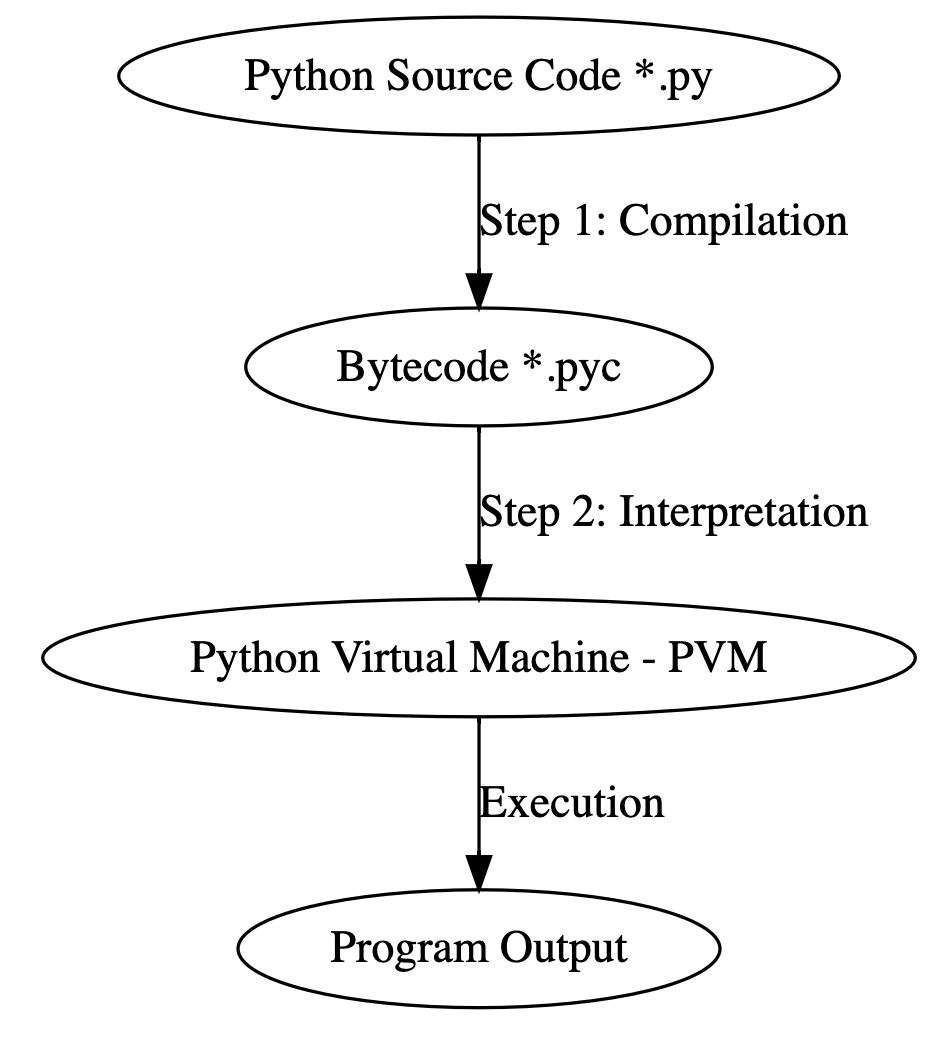
\includegraphics[width=3.125in,height=\textheight,keepaspectratio]{index_files/mediabag/python_scheme.png}

}

\caption{Interpreter Scheme - Simplified}

\end{figure}%

\section*{How I can learn Python?}\label{how-i-can-learn-python}
\addcontentsline{toc}{section}{How I can learn Python?}

\markright{How I can learn Python?}

There are a lot of resources to dive deeper into Python \emph{e.g.}:

\begin{itemize}
\tightlist
\item
  \url{https://www.py4e.com/} (Python for Everybody)
\item
  \url{https://py-tutorial-de.readthedocs.io/de/python-3.3/} (German
  Tutorial)
\item
  \url{https://www.w3schools.com/python/default.asp}
\item
  \url{https://jakevdp.github.io/PythonDataScienceHandbook/}
\item
  \url{https://exercism.org/} (Coding Exercises)
\item
  \url{https://www.freecodecamp.org/} (Coding Exercises)
\item
  \url{https://realpython.com/tutorials/data-viz/}
\item
  \url{https://www.youtube.com/watch?v=LHBE6Q9XlzI}
\end{itemize}

\section*{Use AI to learn Python}\label{use-ai-to-learn-python}
\addcontentsline{toc}{section}{Use AI to learn Python}

\markright{Use AI to learn Python}

\begin{tcolorbox}[enhanced jigsaw, leftrule=.75mm, bottomrule=.15mm, colbacktitle=quarto-callout-important-color!10!white, title=\textcolor{quarto-callout-important-color}{\faExclamation}\hspace{0.5em}{Important}, breakable, arc=.35mm, toptitle=1mm, opacityback=0, titlerule=0mm, coltitle=black, colback=white, opacitybacktitle=0.6, colframe=quarto-callout-important-color-frame, left=2mm, rightrule=.15mm, toprule=.15mm, bottomtitle=1mm]

\begin{itemize}
\item
  Language Models like GPT-3 can help you to learn Python.
\item
  Today it is not always necessary to learn the syntax of a programming
  languages by heart.
\item
  You can use AI tools to help you with the syntax and concentrate on
  the problem-solving part.
\item
  \textbf{Learn how to prompt} your problem to the AI and get a proper
  solution.
\item
  But \textbf{be aware} that the AI is \textbf{not perfect} and can give
  you \textbf{wrong solutions}.
\item
  So it is \textbf{important} that you can \textbf{understand the code}
  and can debug it.
\item
  AI is only a tool not a replacement for a human.
\end{itemize}

\end{tcolorbox}

\section*{Practice, Practice,
Practice}\label{practice-practice-practice}
\addcontentsline{toc}{section}{Practice, Practice, Practice}

\markright{Practice, Practice, Practice}

\begin{tcolorbox}[enhanced jigsaw, leftrule=.75mm, bottomrule=.15mm, colbacktitle=quarto-callout-important-color!10!white, title=\textcolor{quarto-callout-important-color}{\faExclamation}\hspace{0.5em}{Important}, breakable, arc=.35mm, toptitle=1mm, opacityback=0, titlerule=0mm, coltitle=black, colback=white, opacitybacktitle=0.6, colframe=quarto-callout-important-color-frame, left=2mm, rightrule=.15mm, toprule=.15mm, bottomtitle=1mm]

As it is with languages, you can only learn it if you \textbf{practice}
it. So, start you own projects and have fun with it!

\end{tcolorbox}

\chapter{Installation Guide}\label{installation-guide}

Difficulty level: { }

Here is a short instruction how to install Python on your local PC or
you can use \href{https://colab.research.google.com}{Google Colab} to
solve all the exercises of this course.

The use of \href{https://colab.research.google.com}{Google Colab} needs
a Google Account. Please read the
\href{https://research.google.com/colaboratory/tos_v5.html}{Terms of
Service} and \href{https://policies.google.com/privacy}{Privacy Policy}

\chapter*{How to install Python
locally?}\label{how-to-install-python-locally}
\addcontentsline{toc}{chapter}{How to install Python locally?}

\markboth{How to install Python locally?}{How to install Python
locally?}

Fundamental Python websites:

\begin{itemize}
\tightlist
\item
  \href{https://www.python.org}{Python}
\item
  \href{https://www.python.org/doc/}{Python documentation}
\end{itemize}

\section*{1. Install Python Interpreter (you do not needed if you use an
environment
manager)}\label{install-python-interpreter-you-do-not-needed-if-you-use-an-environment-manager}
\addcontentsline{toc}{section}{1. Install Python Interpreter (you do not
needed if you use an environment manager)}

\markright{1. Install Python Interpreter (you do not needed if you use
an environment manager)}

Your preferred searching engine is your friend to find the best way to
install Python on your system. Please choose that method which is
suitable for you.

Python can be installed by several ways:

\begin{itemize}
\tightlist
\item
  directly by \href{https://www.python.org/downloads/}{Python} official
  site

  \begin{itemize}
  \tightlist
  \item
    the installation guide can be found under
    \href{https://wiki.python.org/moin/BeginnersGuide/Download}{python
    wiki}
  \end{itemize}
\item
  or via package manager of your os:

  \begin{itemize}
  \tightlist
  \item
    \emph{e.g.:} \texttt{sudo\ apt\ install\ python} (linux debian) or
    \texttt{brew\ install\ python} (macOS)
  \end{itemize}
\item
  or via \href{https://www.docker.com/}{docker},
  \href{https://learn.microsoft.com/de-de/windows/wsl/install}{wsl} ect.
\item
  or via a
  \href{https://docs.conda.io/projects/conda/en/latest/index.html}{conda}
  or \href{https://mamba.readthedocs.io/en/latest/index.html}{mamba}
  python package and environment managers which have a python
  interpreter on board and are available for Windows, Linux and macOS
  {[}my recommendation{]}
\end{itemize}

\section*{2. Python Package and Environment
manager}\label{python-package-and-environment-manager}
\addcontentsline{toc}{section}{2. Python Package and Environment
manager}

\markright{2. Python Package and Environment manager}

The advantage of using a python package and environment manager is that
you have a python interpreter directly on board, but you can also
directly create different python enviroments and install and remove
python packages.

\subsection*{Conda}\label{conda}
\addcontentsline{toc}{subsection}{Conda}

There are differerent \texttt{conda} installer: (Please pay attention
which one is suitable for you
(\url{https://docs.anaconda.com/distro-or-miniconda/}).

\begin{tcolorbox}[enhanced jigsaw, leftrule=.75mm, bottomrule=.15mm, colbacktitle=quarto-callout-warning-color!10!white, title=\textcolor{quarto-callout-warning-color}{\faExclamationTriangle}\hspace{0.5em}{Warning}, breakable, arc=.35mm, toptitle=1mm, opacityback=0, titlerule=0mm, coltitle=black, colback=white, opacitybacktitle=0.6, colframe=quarto-callout-warning-color-frame, left=2mm, rightrule=.15mm, toprule=.15mm, bottomtitle=1mm]

Please read the
\href{https://www.anaconda.com/pricing/terms-of-service-faqs}{Anaconda
Terms of Service FAQs} and
\href{https://legal.anaconda.com/policies/en/}{Terms of Service})
\textbf{not} every case is \textbf{free} of charge of use.

\end{tcolorbox}

\begin{itemize}
\tightlist
\item
  \href{https://docs.anaconda.com/anaconda/install/}{Anaconda
  Distribution} is a comprehensive distribution which includes conda and
  hundreds of preinstalled packages and tools.
\item
  \href{https://docs.anaconda.com/free/miniconda/index.html}{miniconda}
  is the light version of it which contains only conda, python
  interpreter and few fundamental packages
\item
  \href{https://github.com/conda-forge/miniforge}{miniforge} minimal
  installer for conda and using only the community
  \href{https://conda-forge.org/}{conda-forge} channel
\end{itemize}

\subsection*{Mamba}\label{mamba}
\addcontentsline{toc}{subsection}{Mamba}

Another python package and environment manager is
\href{https://mamba.readthedocs.io/en/latest/index.html}{mamba}.

\texttt{mamba} is a reimplementation of \texttt{conda}:

\begin{itemize}
\tightlist
\item
  \href{https://mamba.readthedocs.io/en/latest/installation/micromamba-installation.html}{micromamba}
  is a statically linked version of \texttt{mamba}
\item
  \texttt{mamba}and it is currently faster than \texttt{conda}
\end{itemize}

\begin{tcolorbox}[enhanced jigsaw, leftrule=.75mm, bottomrule=.15mm, colbacktitle=quarto-callout-tip-color!10!white, title=\textcolor{quarto-callout-tip-color}{\faLightbulb}\hspace{0.5em}{Tip}, breakable, arc=.35mm, toptitle=1mm, opacityback=0, titlerule=0mm, coltitle=black, colback=white, opacitybacktitle=0.6, colframe=quarto-callout-tip-color-frame, left=2mm, rightrule=.15mm, toprule=.15mm, bottomtitle=1mm]

\textbf{Recommendation: \emph{micromamba} }

Install it like it is explained under the micromamba documentation: -
\url{https://mamba.readthedocs.io/en/latest/installation/micromamba-installation.html}

\end{tcolorbox}

Please install in one of the above explained ways Python and use your
preferred searching engine to get more information.

\section*{3. Set up an environment}\label{set-up-an-environment}
\addcontentsline{toc}{section}{3. Set up an environment}

\markright{3. Set up an environment}

It is often very useful to have different python environments for
different python projects because of the need of different python
package versions.

You can use \texttt{conda} or \texttt{micromamba} to create different
environments. There exists also other virtual environment manager.

In this course the explanation is restricted to \texttt{micromamba} as
an example. If you want to use something else there exists tons of
information online how to use other programs.

\subsection*{Micromamba: Most important commands
are:}\label{micromamba-most-important-commands-are}
\addcontentsline{toc}{subsection}{Micromamba: Most important commands
are:}

Read for more detail:
\url{https://mamba.readthedocs.io/en/latest/user_guide/micromamba.html}

Creating a new virtual environment:

\begin{Shaded}
\begin{Highlighting}[]
\ExtensionTok{micromamba}\NormalTok{ create }\AttributeTok{{-}{-}name} \OperatorTok{\textless{}}\NormalTok{myenvname}\OperatorTok{\textgreater{}}
\end{Highlighting}
\end{Shaded}

Install new packages:

\begin{Shaded}
\begin{Highlighting}[]
\ExtensionTok{micromamba}\NormalTok{ install }\OperatorTok{\textless{}}\NormalTok{packagename}\OperatorTok{\textgreater{}}
\end{Highlighting}
\end{Shaded}

List all environments:

\begin{Shaded}
\begin{Highlighting}[]
\ExtensionTok{micromamba}\NormalTok{ env list}
\end{Highlighting}
\end{Shaded}

Activate an environment:

\begin{Shaded}
\begin{Highlighting}[]
\ExtensionTok{micromamba}\NormalTok{ activate }\OperatorTok{\textless{}}\NormalTok{myenvname}\OperatorTok{\textgreater{}}
\end{Highlighting}
\end{Shaded}

List all packages of this environment:

\begin{Shaded}
\begin{Highlighting}[]
\ExtensionTok{micromamba}\NormalTok{ list}
\end{Highlighting}
\end{Shaded}

\section*{4. Usefull packages for Data Analysis and
Visualization:}\label{usefull-packages-for-data-analysis-and-visualization}
\addcontentsline{toc}{section}{4. Usefull packages for Data Analysis and
Visualization:}

\markright{4. Usefull packages for Data Analysis and Visualization:}

\begin{itemize}
\tightlist
\item
  \href{https://packaging.python.org/en/latest/guides/tool-recommendations/}{pip}
  - package installer for python instead of conda
\item
  \href{https://jupyter.org/}{jupyter-notebook/jupyterlab} - interactive
  computing environment
\item
  \href{https://pypi.org/project/ipykernel/}{ipykernel} - IPython Kernel
  for Jupyter
\item
  \href{https://matplotlib.org}{matplotlib} - data visualization library
\item
  \href{https://numpy.org}{numpy} - numerical library
\item
  \href{https://docs.scipy.org/doc/scipy/reference/}{scipy} - scientific
  library
\item
  \href{https://pandas.pydata.org/docs/}{pandas} - data manipulation
  library
\item
  \href{https://seaborn.pydata.org/examples/index.html}{seaborn} - data
  visualization library
\item
  \href{https://scikit-learn.org/stable/}{scikit-learn} - machine
  learning library
\item
  \href{https://www.statsmodels.org/stable/index.html}{statsmodels} -
  statistical library
\end{itemize}

\textbf{special packages for data visualization:}

\begin{itemize}
\tightlist
\item
  \href{https://docs.bokeh.org/en/latest/index.html}{bokeh} -
  interactive data visualization library
\item
  \href{https://plotly.com/python/}{plotly} - interactive data
  visualization library
\item
  \href{https://networkx.org/documentation/stable/}{networkx} - network
  analysis library
\item
  \href{https://python-ternary.readthedocs.io/en/latest/}{python-ternary}
  - ternary plot library
\item
  \href{https://altair-viz.github.io/}{altair} - declarative statistical
  visualization library
\item
  \href{https://umap-learn.readthedocs.io/en/latest/}{umap-learn} -
  dimensionality reduction library
\end{itemize}

\textbf{special packages for chemistry and material science:}

\begin{itemize}
\tightlist
\item
  \href{https://wiki.fysik.dtu.dk/ase/}{ase} - atomic simulation
  environment
\item
  \href{https://pymatgen.org/}{pymatgen} - Python Materials Genomics
\item
  \href{https://www.rdkit.org/docs/index.html}{RdKit} - cheminformatics
  library
\item
  \href{https://openbabel.org/index.html}{openbabel} - cheminformatics
  library
\item
  \href{https://pymol.org/\#opensource}{pymol-opensource} - molecular
  visualization library
\end{itemize}

For more chemistry and material science packages please check the
\href{https://github.com/lmmentel/awesome-python-chemistry}{Awesome
Python Chemistry} repository.

\section*{Short Cut}\label{short-cut}
\addcontentsline{toc}{section}{Short Cut}

\markright{Short Cut}

\begin{tcolorbox}[enhanced jigsaw, leftrule=.75mm, bottomrule=.15mm, colbacktitle=quarto-callout-tip-color!10!white, title=\textcolor{quarto-callout-tip-color}{\faLightbulb}\hspace{0.5em}{Tip}, breakable, arc=.35mm, toptitle=1mm, opacityback=0, titlerule=0mm, coltitle=black, colback=white, opacitybacktitle=0.6, colframe=quarto-callout-tip-color-frame, left=2mm, rightrule=.15mm, toprule=.15mm, bottomtitle=1mm]

\textbf{Recommendation} Use \emph{yml-file} with all needed packages and
configurations:

\end{tcolorbox}

Save your needed packages in an \texttt{environment.yml} file
\emph{e.g.}:

\begin{Shaded}
\begin{Highlighting}[]
\NormalTok{name: myenv}
\NormalTok{channels:}
\NormalTok{ {-} conda{-}forge}
\NormalTok{dependencies:}
\NormalTok{ {-} python=3.12}
\NormalTok{ {-} pip}
\NormalTok{ {-} ipykernel}
\NormalTok{ {-} jupyterlab}
\NormalTok{ {-} pandas}
\NormalTok{ {-} numpy}
\NormalTok{ {-} matplotlib}
\NormalTok{ {-} scikit{-}learn}
\NormalTok{ {-} scipy}
\NormalTok{ {-} seaborn}
\NormalTok{ {-} statsmodels}
\end{Highlighting}
\end{Shaded}

and create an environment with this specific packages:

\begin{Shaded}
\begin{Highlighting}[]
\ExtensionTok{micromamba}\NormalTok{ env create }\AttributeTok{{-}f}\NormalTok{ environment.yml}
\end{Highlighting}
\end{Shaded}

Then you can activate it via:

\begin{Shaded}
\begin{Highlighting}[]
\ExtensionTok{micromamba}\NormalTok{ activate myenv}
\end{Highlighting}
\end{Shaded}

\section*{5. Test your installation}\label{test-your-installation}
\addcontentsline{toc}{section}{5. Test your installation}

\markright{5. Test your installation}

Test your installation by opening the interactive python mode by typing
in your terminal (Linux, macOS) / command prompt (Windows):

\begin{Shaded}
\begin{Highlighting}[]
\ExtensionTok{python}
\end{Highlighting}
\end{Shaded}

then something like this should be opened in your terminal (Linux,
macOS) / command prompt (Windows)

\begin{Shaded}
\begin{Highlighting}[]
\ExtensionTok{Python}\NormalTok{ 3.12.7 }\KeywordTok{|} \ExtensionTok{packaged}\NormalTok{ by conda{-}forge }\KeywordTok{|} \KeywordTok{(}\ExtensionTok{main,}\NormalTok{ Oct  4 2024, 15:57:01}\KeywordTok{)} \ExtensionTok{[Clang}\NormalTok{ 17.0.6 ] on darwin}
\ExtensionTok{Type} \StringTok{"help"}\NormalTok{, }\StringTok{"copyright"}\NormalTok{, }\StringTok{"credits"}\NormalTok{ or }\StringTok{"license"}\NormalTok{ for more information.}
\OperatorTok{\textgreater{}\textgreater{}\textgreater{}} 
\end{Highlighting}
\end{Shaded}

then type:

\begin{Shaded}
\begin{Highlighting}[]
\BuiltInTok{print}\NormalTok{(}\StringTok{"Hello World!"}\NormalTok{)}
\end{Highlighting}
\end{Shaded}

If this works your installation was successful!

\chapter{Editors}\label{editors}

Difficulty level: { }

\chapter*{Choose an editor}\label{choose-an-editor}
\addcontentsline{toc}{chapter}{Choose an editor}

\markboth{Choose an editor}{Choose an editor}

After you installed Python successfully you need an editor for writing
your Python programs. A python script is a text file with the ending
\texttt{.py}. Technicallly you could use everything where you can write
text, but it is not really purposeful.

An editor with \textbf{syntax highlighting}, \textbf{code completion}
and \textbf{debugging} is very useful.

\subsection*{Editors:}\label{editors-1}
\addcontentsline{toc}{subsection}{Editors:}

\begin{itemize}
\tightlist
\item
  Spyder \url{https://www.spyder-ide.org/}
\item
  PyCharm (JetBrains)
  \url{https://www.jetbrains.com/products/compare/?product=pycharm&product=pycharm-ce}
\item
  Jupyter Notebook \url{https://jupyter.org/}
  \url{https://code.visualstudio.com/docs/datascience/jupyter-notebooks}
\item
  Jupyter Lab \url{https://jupyter.org/}
  \url{https://code.visualstudio.com/docs/datascience/jupyter-notebooks}
\item
  Google Google Colab \url{https://colab.research.google.com/} etc.
\end{itemize}

\begin{tcolorbox}[enhanced jigsaw, leftrule=.75mm, bottomrule=.15mm, colbacktitle=quarto-callout-tip-color!10!white, title=\textcolor{quarto-callout-tip-color}{\faLightbulb}\hspace{0.5em}{Tip}, breakable, arc=.35mm, toptitle=1mm, opacityback=0, titlerule=0mm, coltitle=black, colback=white, opacitybacktitle=0.6, colframe=quarto-callout-tip-color-frame, left=2mm, rightrule=.15mm, toprule=.15mm, bottomtitle=1mm]

\textbf{Recommendation}:
\emph{\href{https://code.visualstudio.com/download}{Visual Studio Code}}

\end{tcolorbox}

\subsection*{Python extension for VS
Code:}\label{python-extension-for-vs-code}
\addcontentsline{toc}{subsection}{Python extension for VS Code:}

\begin{itemize}
\tightlist
\item
  Python from Microsoft,
\item
  Pylance from Microsoft
\item
  and Jupyter from Microsoft (optional it is only needed if you want to
  use Jupyter Notebooks in VS Code)
\end{itemize}

Alternatively you can use a \texttt{Jupyter\ Notebook}
(\texttt{*.ipynb}) to execute code. Jupyter Notebooks are interactive
documents that allow you to write and execute Python code line by line.
In comparison to a Python script, which is a plain text file with the
\texttt{.py} extension, Jupyter Notebooks provide a more user-friendly
interface for data analysis and visualization.

Write the code in a cell and execute it by pressing the run button.

\textbf{Advantage of using Jupyter Notebooks}:

\begin{itemize}
\tightlist
\item
  The code can run cell by cell and the output is directly shown below
  the cell.
\item
  Further you can write text and equations in markdown cells.
\item
  Jupyter Notebooks can also handle different programming languages like
  \texttt{R}or \texttt{Julia}.
\item
  Also \texttt{Markdown} and \texttt{LaTeX} can be used to write text
  and equations.
\item
  The output of the code can be visualized directly in the notebook.
\item
  Therefore, it is very popular in the data science community.
\end{itemize}

Jupyter Notebooks can be used in \texttt{VS\ Code},
\texttt{Jupyter\ Lab}, \texttt{Jupyter\ Notebook} or
\texttt{Google\ Colab}.

In this course all exercises are provided as Jupyter Notebooks. You can
download it or run it directly in Google Colab.

\section*{Using Jupyter Notebooks in VS
Code}\label{using-jupyter-notebooks-in-vs-code}
\addcontentsline{toc}{section}{Using Jupyter Notebooks in VS Code}

\markright{Using Jupyter Notebooks in VS Code}

\begin{figure}[H]

{\centering \pandocbounded{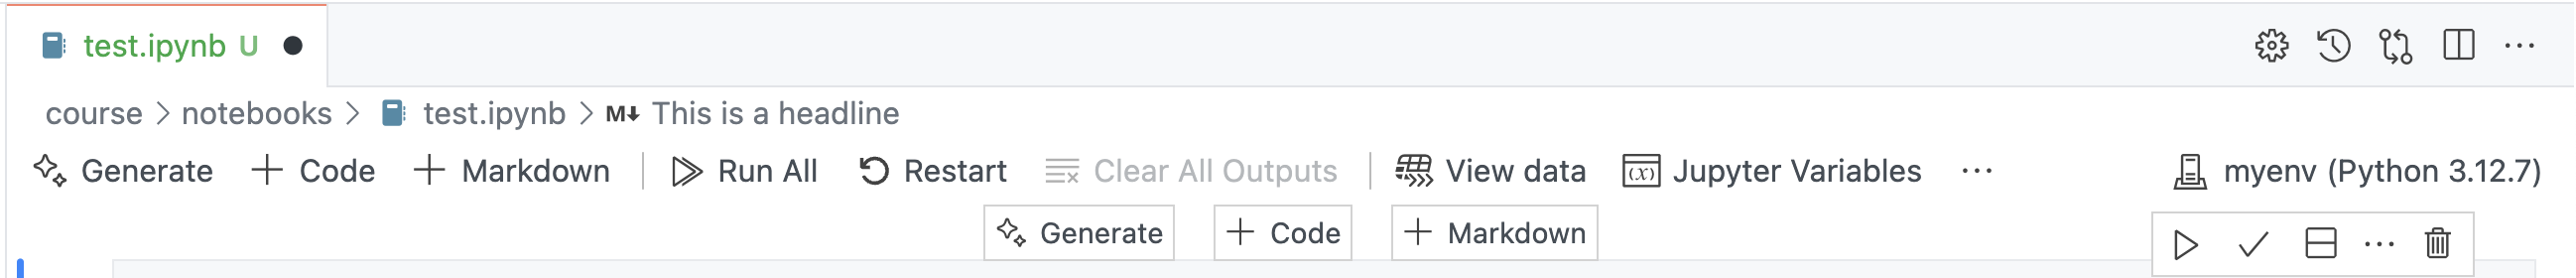
\includegraphics[keepaspectratio]{index_files/mediabag/ipynb-vscode.png}}

}

\caption{VS Code}

\end{figure}%%
\begin{figure}[H]

{\centering \pandocbounded{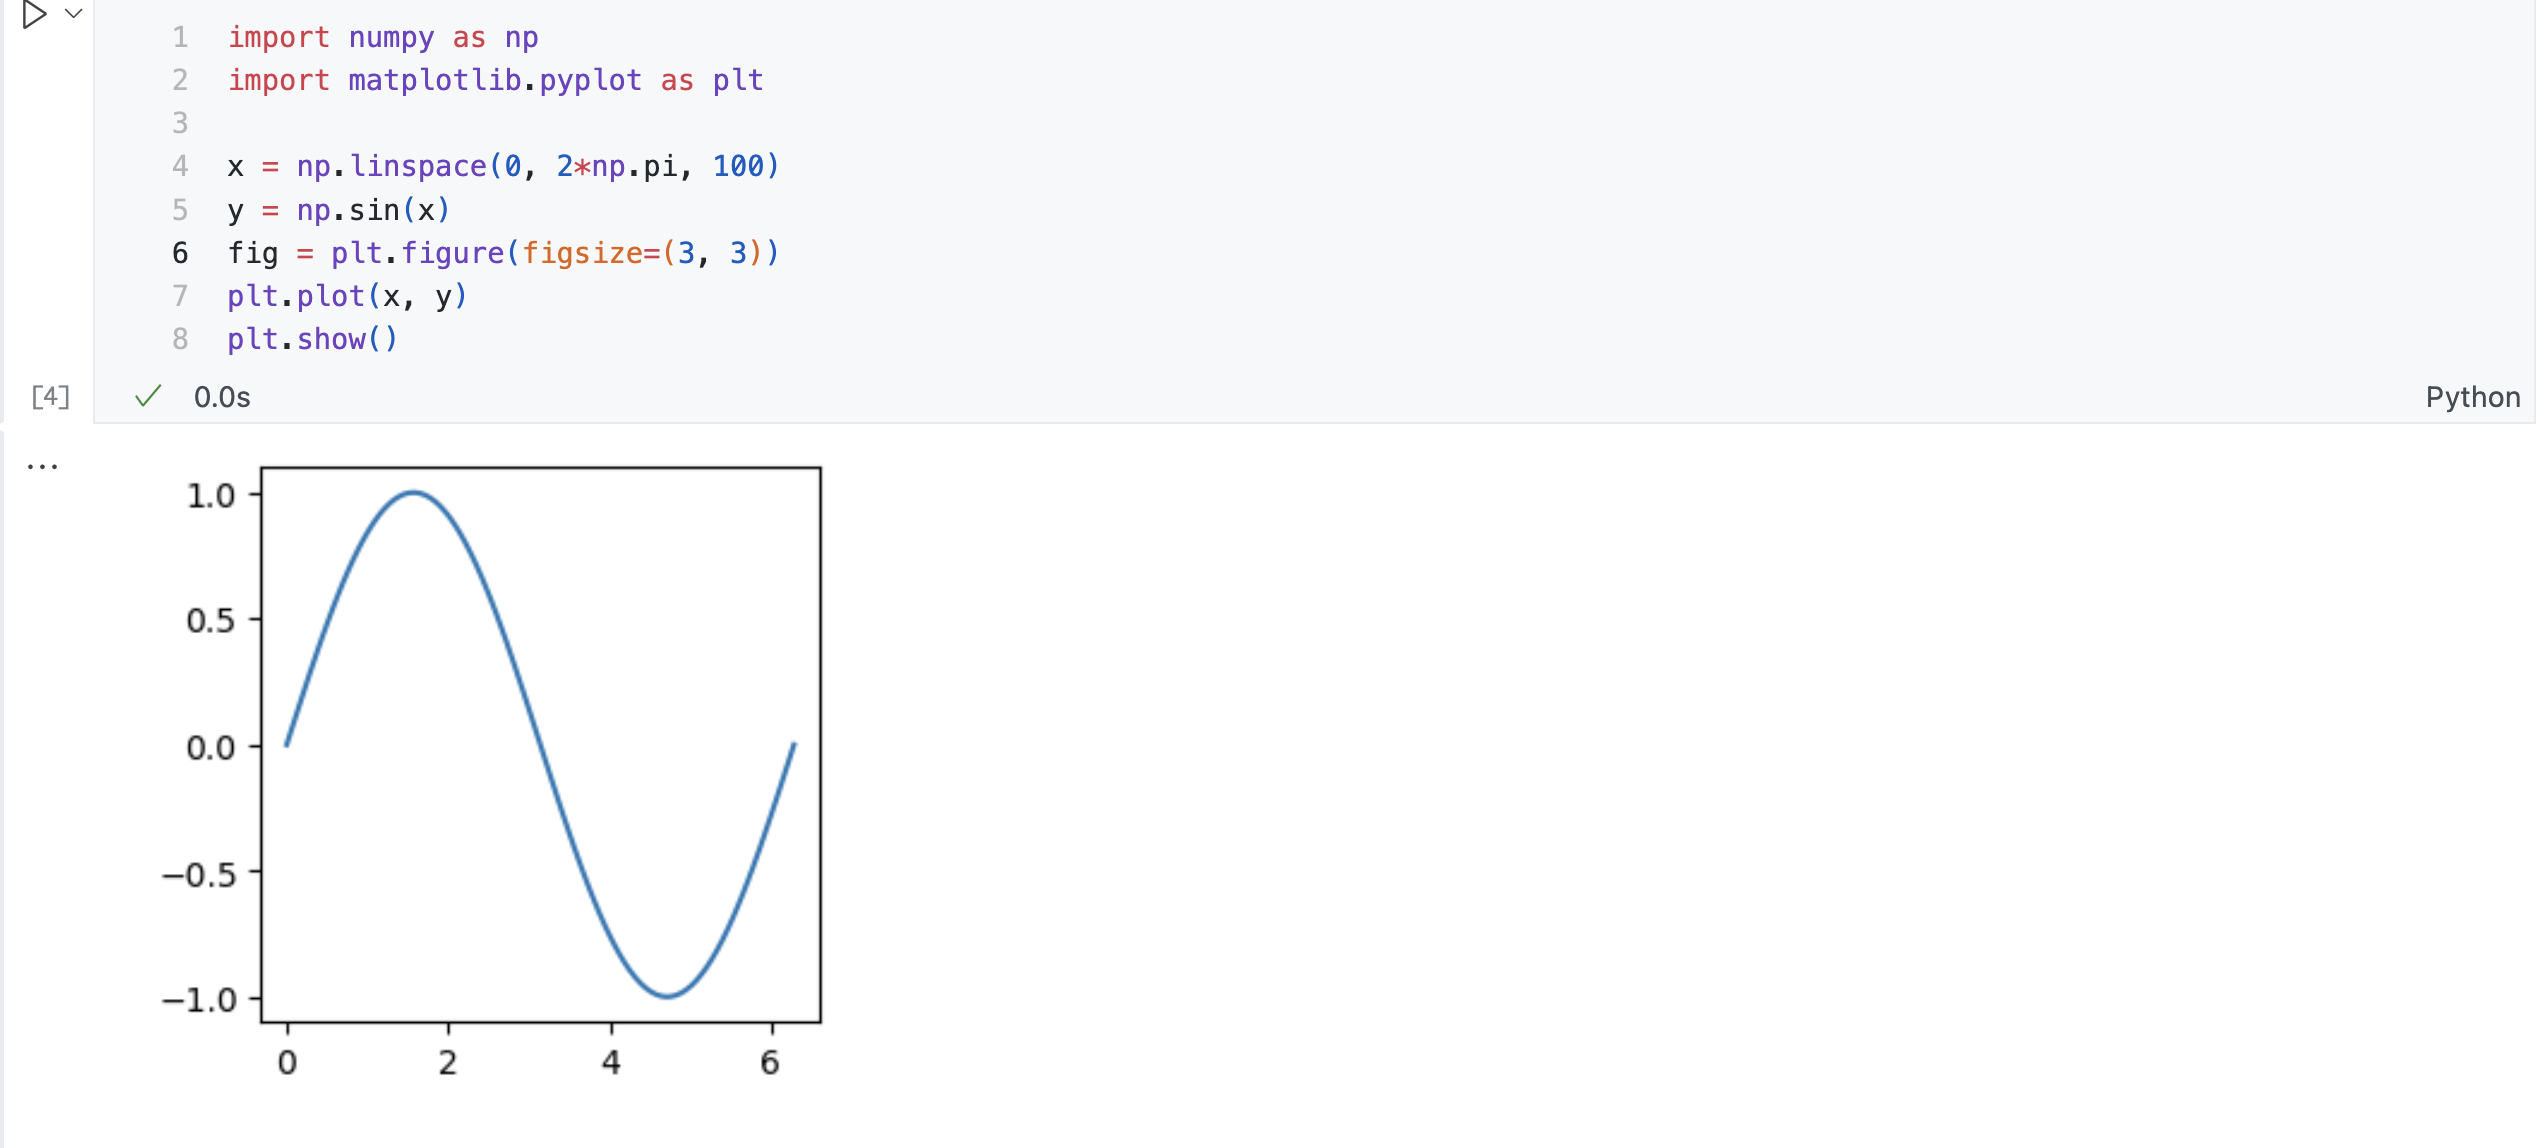
\includegraphics[keepaspectratio]{index_files/mediabag/python.png}}

}

\caption{Python Cell}

\end{figure}%

\subsection{Difference Between Jupyter Notebooks and Python
Scripts}\label{difference-between-jupyter-notebooks-and-python-scripts}

\begin{itemize}
\tightlist
\item
  \textbf{Interactivity}: Jupyter Notebooks allow you to run code in
  chunks (cells) and see the output immediately, making them ideal for
  experimentation and visualization. Python scripts (\texttt{.py} files)
  are typically executed all at once.
\item
  \textbf{Documentation}: Notebooks support Markdown cells for adding
  rich text, equations, and images alongside your code. Python scripts
  are plain text files and require comments for documentation.
\item
  \textbf{Use Case}: Notebooks are great for exploratory data analysis
  and teaching, while Python scripts are better suited for production
  code and automation.
\end{itemize}

\section{Google Colab Tutorial}\label{google-colab-tutorial}

Google Colab is a free, cloud-based platform that allows you to run
Jupyter Notebooks without any setup. To get started with Google Colab:

The use of \href{https://colab.research.google.com}{Google Colab} needs
a Google Account. Please read the
\href{https://research.google.com/colaboratory/tos_v5.html}{Terms of
Service} and \href{https://policies.google.com/privacy}{Privacy Policy}

\begin{enumerate}
\def\labelenumi{\arabic{enumi}.}
\tightlist
\item
  Visit \href{https://colab.research.google.com/}{Google Colab} and sign
  in with your Google account.
\item
  Create a new notebook or upload an existing \texttt{.ipynb} file.
\item
  Write and execute code in cells, just like in Jupyter Notebooks.
\item
  Save your work to Google Drive or download it as a \texttt{.ipynb}
  file.
\end{enumerate}

\subsection{Key Features of Google
Colab}\label{key-features-of-google-colab}

\begin{itemize}
\tightlist
\item
  \textbf{Free Access to GPUs/TPUs}: Accelerate your computations by
  enabling GPU or TPU support from the ``Runtime'' menu.
\item
  \textbf{Collaboration}: Share notebooks with others and work on them
  simultaneously, similar to Google Docs.
\item
  \textbf{Pre-installed Libraries}: Many popular Python libraries are
  pre-installed, saving you setup time.
\item
  \textbf{Integration with Google Drive}: Easily access and save files
  to your Google Drive.
\end{itemize}

\begin{figure}[H]

{\centering \pandocbounded{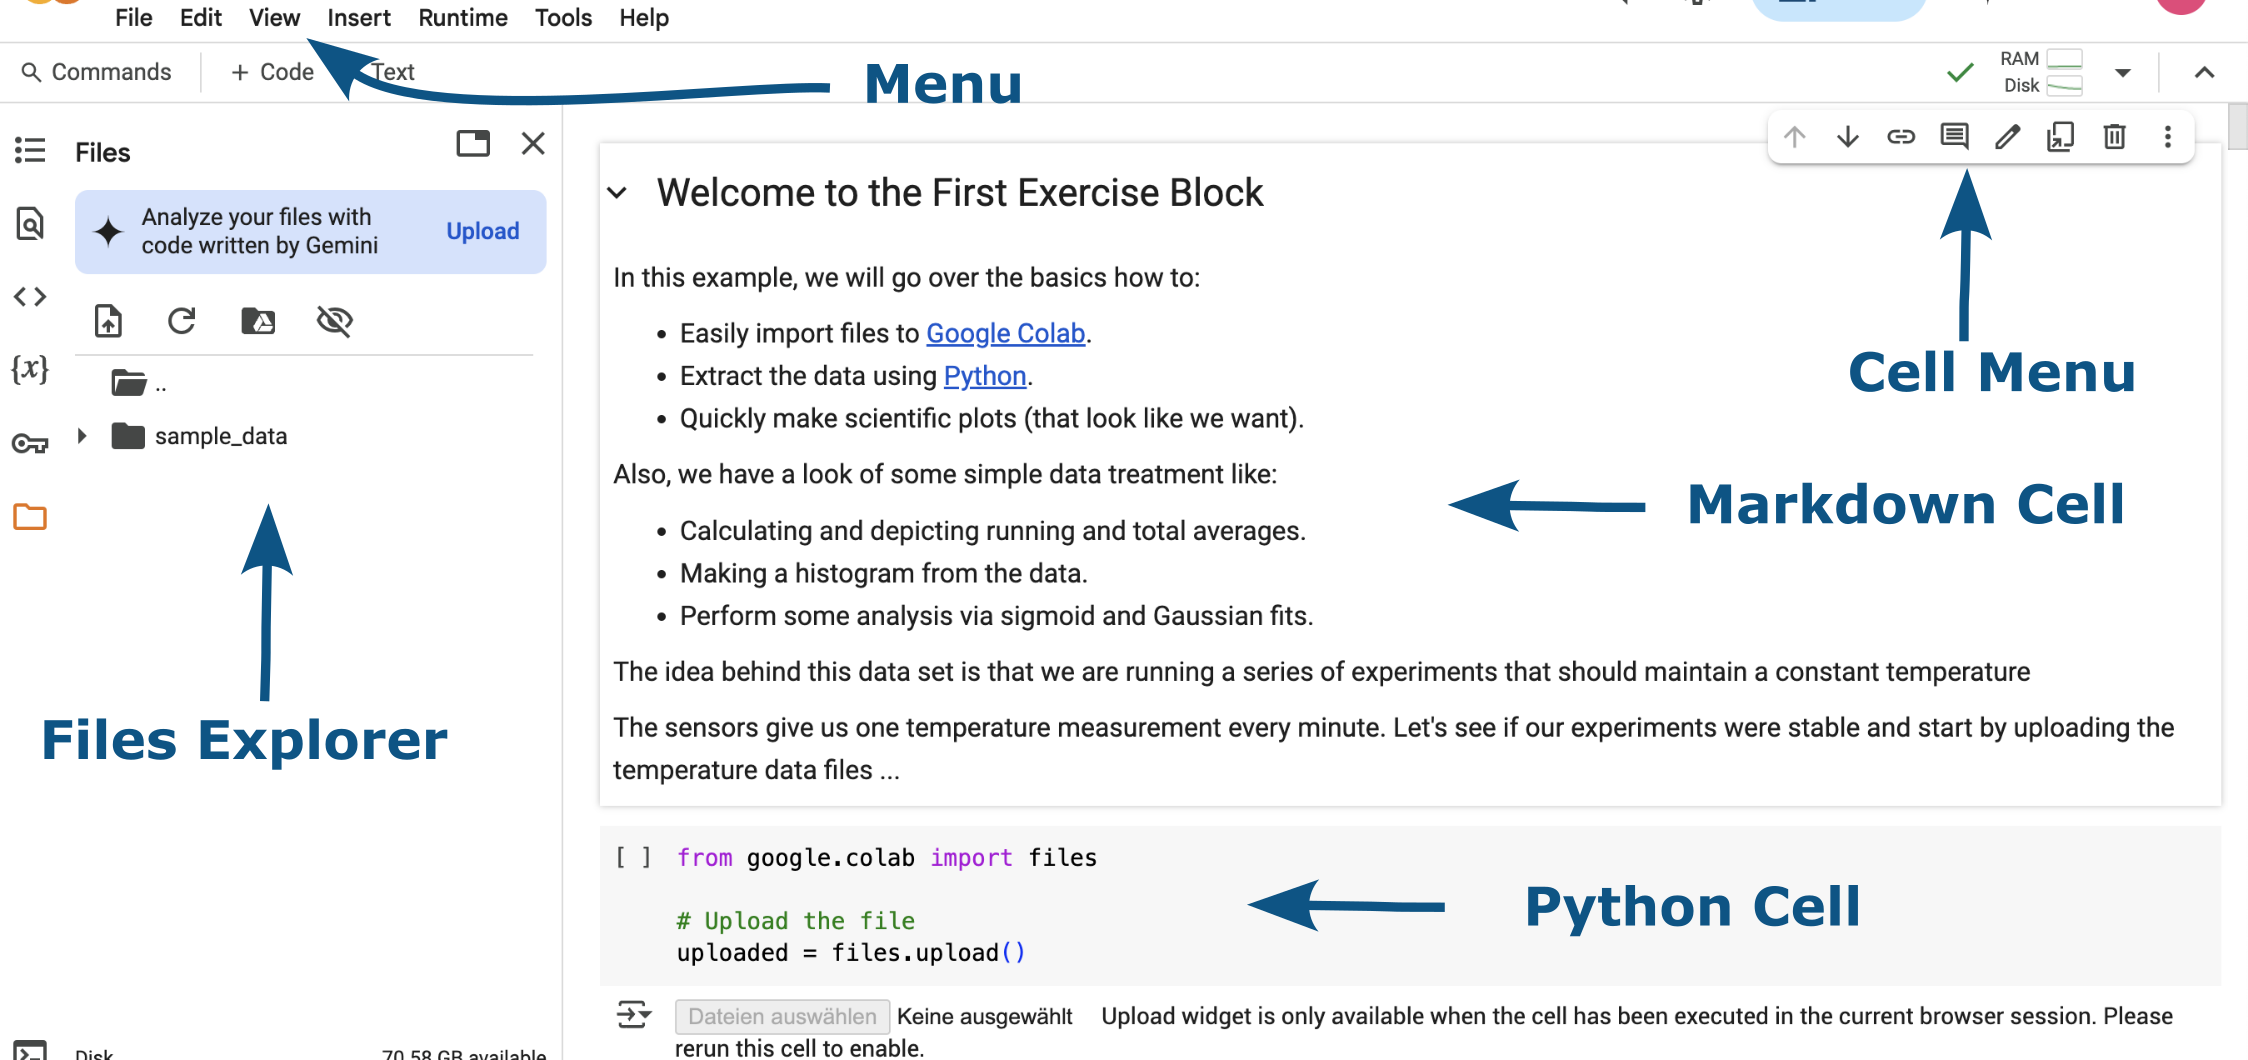
\includegraphics[keepaspectratio]{index_files/mediabag/googlecolab.png}}

}

\caption{Google Colab Interface}

\end{figure}%

Upload data on Google Colab:

\begin{Shaded}
\begin{Highlighting}[]
\ImportTok{from}\NormalTok{ google.colab }\ImportTok{import}\NormalTok{ files}
\end{Highlighting}
\end{Shaded}

\subsection{Upload a file}\label{upload-a-file}

\begin{Shaded}
\begin{Highlighting}[]
\NormalTok{uploaded }\OperatorTok{=}\NormalTok{ files.upload()}
\end{Highlighting}
\end{Shaded}

\subsection{Access the uploaded file}\label{access-the-uploaded-file}

\begin{Shaded}
\begin{Highlighting}[]
\ControlFlowTok{for}\NormalTok{ filename }\KeywordTok{in}\NormalTok{ uploaded.keys():}
    \BuiltInTok{print}\NormalTok{(}\SpecialStringTok{f\textquotesingle{}User uploaded file "}\SpecialCharTok{\{}\NormalTok{filename}\SpecialCharTok{\}}\SpecialStringTok{" with size }\SpecialCharTok{\{}\BuiltInTok{len}\NormalTok{(uploaded[filename])}\SpecialCharTok{\}}\SpecialStringTok{ bytes.\textquotesingle{}}\NormalTok{)}\CommentTok{\#}
\end{Highlighting}
\end{Shaded}

\subsection{Important Short Cuts in Google
Colab}\label{important-short-cuts-in-google-colab}

\begin{itemize}
\tightlist
\item
  \textbf{Run cell and select next cell}: \texttt{Shift\ +\ Enter}
\item
  \textbf{Run focused celll}: \texttt{⌘/Ctrl\ +\ Enter}
\item
  \textbf{Insert cell below}: \texttt{⌘/Ctrl\ +\ M\ B}
\item
  \textbf{Insert cell above}: \texttt{⌘/Ctrl\ +\ M\ A}
\item
  \textbf{Delete cell}: \texttt{⌘/Ctrl\ +\ M\ D}
\item
  \textbf{Undo last action}: \texttt{⌘/Ctrl\ +\ M\ Z}
\item
  \textbf{Comment/Uncomment line}: \texttt{⌘/Ctrl\ +\ Alt\ +\ M}
\item
  \textbf{Find and replace}: \texttt{⌘/Ctrl\ +\ H}
\item
  \textbf{Show keyboard shortcuts}: \texttt{⌘/Ctrl\ +\ K\ H}
\end{itemize}

\begin{center}\rule{0.5\linewidth}{0.5pt}\end{center}

\chapter*{Test your chosen setup}\label{test-your-chosen-setup}
\addcontentsline{toc}{chapter}{Test your chosen setup}

\markboth{Test your chosen setup}{Test your chosen setup}

\begin{itemize}
\tightlist
\item
  open your editor
\item
  open a new file and save this file as helloworld.py
\item
  write your first test program:
\end{itemize}

\begin{Shaded}
\begin{Highlighting}[]
\BuiltInTok{print}\NormalTok{(}\StringTok{"Hello World!"}\NormalTok{)}
\end{Highlighting}
\end{Shaded}

\begin{itemize}
\tightlist
\item
  execute your program by using your IDE/Editor
\item
  or using command line in the terminal (Linux/MacOS) / command prompt
  under Windows.
\end{itemize}

\begin{Shaded}
\begin{Highlighting}[]
\BuiltInTok{cd}\NormalTok{ /path/to/file}
\ExtensionTok{python}\NormalTok{ helloworld.py}
\end{Highlighting}
\end{Shaded}

The ouput should be: ``Hello World!''.

If you are using Jupyter Notebook you can also write this code in a cell
and execute it by pressing the run button.

\begin{tcolorbox}[enhanced jigsaw, leftrule=.75mm, bottomrule=.15mm, colbacktitle=quarto-callout-tip-color!10!white, title={Tip}, breakable, arc=.35mm, toptitle=1mm, opacityback=0, titlerule=0mm, coltitle=black, colback=white, opacitybacktitle=0.6, colframe=quarto-callout-tip-color-frame, left=2mm, rightrule=.15mm, toprule=.15mm, bottomtitle=1mm]

Congratulations \textbf{You have successfully set up python!!}

\end{tcolorbox}

\part{Python Crash Course}

\chapter{Python Start}\label{python-start}

Difficulty level: { }

This will be a very fast and basic start into coding with Python.

\begin{tcolorbox}[enhanced jigsaw, leftrule=.75mm, bottomrule=.15mm, colbacktitle=quarto-callout-note-color!10!white, title=\textcolor{quarto-callout-note-color}{\faInfo}\hspace{0.5em}{Let`s make an initial quiz.}, breakable, arc=.35mm, toptitle=1mm, opacityback=0, titlerule=0mm, coltitle=black, colback=white, opacitybacktitle=0.6, colframe=quarto-callout-note-color-frame, left=2mm, rightrule=.15mm, toprule=.15mm, bottomtitle=1mm]

You will see coding with Python is very easy and intuitive!

Please remember you can always open this file in \texttt{Google\ Colab}
\href{https://colab.research.google.com/github/stkroe/PythonForChemists/blob/main/course/notebooks/Basics.ipynb}{}
or download it and run it on your local machine
\href{https://github.com/stkroe/PythonforChemists/blob/main/course/notebooks/Basics.ipynb}{}.

\end{tcolorbox}

\begin{tcolorbox}[enhanced jigsaw, leftrule=.75mm, bottomrule=.15mm, colbacktitle=quarto-callout-note-color!10!white, title=\textcolor{quarto-callout-note-color}{\faInfo}\hspace{0.5em}{Quiz}, breakable, arc=.35mm, toptitle=1mm, opacityback=0, titlerule=0mm, coltitle=black, colback=white, opacitybacktitle=0.6, colframe=quarto-callout-note-color-frame, left=2mm, rightrule=.15mm, toprule=.15mm, bottomtitle=1mm]

\phantomsection\label{quiz-container}

\end{tcolorbox}

\chapter*{Elementary Syntax}\label{elementary-syntax}
\addcontentsline{toc}{chapter}{Elementary Syntax}

\markboth{Elementary Syntax}{Elementary Syntax}

\section*{Commands}\label{commands}
\addcontentsline{toc}{section}{Commands}

\markright{Commands}

Each line of code is a command. The computer reads the code from top to
bottom and executes each command in succession order.

First some terminology:

\begin{longtable}[]{@{}
  >{\raggedright\arraybackslash}p{(\linewidth - 2\tabcolsep) * \real{0.2500}}
  >{\raggedright\arraybackslash}p{(\linewidth - 2\tabcolsep) * \real{0.7500}}@{}}
\toprule\noalign{}
\begin{minipage}[b]{\linewidth}\raggedright
Term
\end{minipage} & \begin{minipage}[b]{\linewidth}\raggedright
Definition
\end{minipage} \\
\midrule\noalign{}
\endhead
\bottomrule\noalign{}
\endlastfoot
Command & \emph{A line of code that tells the computer to do
something.} \\
Syntax & \emph{The rules that govern how commands are written.} \\
Execute & \emph{To run a command.} \\
Comment & \emph{A note in the code that is not executed.} \\
Indentation & \emph{The space at the beginning of a line of code that
tells the computer that the line is part of a block of code.} \\
Error & \emph{A message that tells you that something is wrong with your
code.} \\
Stack trace & \emph{A list of error messages that Python prints when an
error occurs.} \\
Variable & \emph{A name that stores a value.} \\
Data type & \emph{The type of value that a variable stores.} \\
Declaration & \emph{The process of assigning memory to a variable.} \\
Integer & \emph{A whole number.} \\
Float & \emph{A number with a decimal point.} \\
Boolean & \emph{A value that is either True or False.} \\
List & \emph{A collection of items.} \\
String & \emph{A sequence of characters.} \\
Function & \emph{A block of code that performs a specific task.} \\
Argument & \emph{A value that is passed to a function.} \\
Parameter & \emph{A variable that is used in a function.} \\
Return & \emph{The value that a function returns.} \\
Keyword Arguments & \emph{Arguments that are passed to a function by
name.} \\
Positional Arguments & \emph{Arguments that are passed to a function by
position.} \\
Default Argument & \emph{An argument that has a default value.} \\
Operator & \emph{A symbol that performs a specific operation.} \\
Expression & \emph{A combination of values and operators that evaluates
to a value.} \\
Statement & \emph{A line of code that performs an action.} \\
Block & \emph{A group of statements that are executed together.} \\
Method & \emph{A function that is associated with an object.} \\
Class & \emph{A blueprint for creating objects.} \\
Object & \emph{An instance of a class.} \\
Instance & \emph{A specific object created from a class.} \\
Mutable & \emph{A type of object that can be changed.} \\
Immutable & \emph{A type of object that cannot be changed.} \\
Module & \emph{A collection of functions and variables.} \\
Library & \emph{A collection of modules.} \\
Package & \emph{A collection of related modules.} \\
Script & \emph{A file that contains code that can be run
independently.} \\
\end{longtable}

\begin{tcolorbox}[enhanced jigsaw, leftrule=.75mm, bottomrule=.15mm, colbacktitle=quarto-callout-note-color!10!white, title=\textcolor{quarto-callout-note-color}{\faInfo}\hspace{0.5em}{Example - Hello World}, breakable, arc=.35mm, toptitle=1mm, opacityback=0, titlerule=0mm, coltitle=black, colback=white, opacitybacktitle=0.6, colframe=quarto-callout-note-color-frame, left=2mm, rightrule=.15mm, toprule=.15mm, bottomtitle=1mm]

\texttt{print} is a command that tells the computer to display the text
or variable that follows it.

\end{tcolorbox}

Try it out:

\begin{itemize}
\tightlist
\item
  Copy the code below and paste it into a code cell.
\item
  Or open this file in \texttt{Google\ Colab} and run the code.
\item
  Or download this file and run it on your local machine.
\end{itemize}

\begin{Shaded}
\begin{Highlighting}[]
\BuiltInTok{print}\NormalTok{(}\StringTok{"Hello World"}\NormalTok{)}
\end{Highlighting}
\end{Shaded}

\begin{verbatim}
Hello World
\end{verbatim}

If you want to span a command over multiple lines you can use
\texttt{\textbackslash{}} or if you are using parenthesis in your
command you can directly use a new line.

\begin{Shaded}
\begin{Highlighting}[]
\NormalTok{ result }\OperatorTok{=} \DecValTok{1} \OperatorTok{+} \DecValTok{2} \OperatorTok{+} \DecValTok{3} \OperatorTok{+} \OperatorTok{\textbackslash{}}
          \DecValTok{7} \OperatorTok{+} \DecValTok{8} \OperatorTok{+} \DecValTok{9}
\NormalTok{ numbers }\OperatorTok{=}\NormalTok{ [}
     \DecValTok{1}\NormalTok{, }\DecValTok{2}\NormalTok{, }\DecValTok{3}\NormalTok{,}
     \DecValTok{4}\NormalTok{, }\DecValTok{5}\NormalTok{, }\DecValTok{6}\NormalTok{,}
     \DecValTok{7}\NormalTok{, }\DecValTok{8}\NormalTok{, }\DecValTok{9}
\NormalTok{ ]}
\end{Highlighting}
\end{Shaded}

\section*{Indentation}\label{indentation}
\addcontentsline{toc}{section}{Indentation}

\markright{Indentation}

In Python code blocks are not structured by brackets or semicolons like
\texttt{C/C++} or \texttt{Java} but by indentation. This means that the
code inside a loop or a function is indented by a tab or spaces.

\begin{tcolorbox}[enhanced jigsaw, leftrule=.75mm, bottomrule=.15mm, colbacktitle=quarto-callout-warning-color!10!white, title=\textcolor{quarto-callout-warning-color}{\faExclamationTriangle}\hspace{0.5em}{Warning}, breakable, arc=.35mm, toptitle=1mm, opacityback=0, titlerule=0mm, coltitle=black, colback=white, opacitybacktitle=0.6, colframe=quarto-callout-warning-color-frame, left=2mm, rightrule=.15mm, toprule=.15mm, bottomtitle=1mm]

Indentations are crucial in Python. If you don't indent your code
correctly, you will get a typical beginner error.

Pay attention \textbf{do not mix tabs and spaces} in your code.

\end{tcolorbox}

\begin{tcolorbox}[enhanced jigsaw, leftrule=.75mm, bottomrule=.15mm, colbacktitle=quarto-callout-note-color!10!white, title=\textcolor{quarto-callout-note-color}{\faInfo}\hspace{0.5em}{Example - Wrong Indentation}, breakable, arc=.35mm, toptitle=1mm, opacityback=0, titlerule=0mm, coltitle=black, colback=white, opacitybacktitle=0.6, colframe=quarto-callout-note-color-frame, left=2mm, rightrule=.15mm, toprule=.15mm, bottomtitle=1mm]

\end{tcolorbox}

Try it out:

\begin{Shaded}
\begin{Highlighting}[]
\BuiltInTok{print}\NormalTok{(}\StringTok{"correct indentation"}\NormalTok{)}
    \BuiltInTok{print}\NormalTok{(}\StringTok{"wrong indentation"}\NormalTok{)}
\end{Highlighting}
\end{Shaded}

\begin{Highlighting}
\textcolor{black}{IndentationError: unexpected indent (1842851760.py, line 2)}
\textcolor{black}{}\textcolor{QuartoInternalColor1}{  Cell }\textcolor{QuartoInternalColor2}{In[3], line 2}\textcolor{QuartoInternalColor1}{}\textcolor{QuartoInternalColor3}{}
\textcolor{QuartoInternalColor3}{}\textcolor{QuartoInternalColor4}{    print("wrong indentation")}\textcolor{QuartoInternalColor3}{}
\textcolor{QuartoInternalColor3}{}\textcolor{QuartoInternalColor3}{    ^}\textcolor{QuartoInternalColor3}{}
\textcolor{QuartoInternalColor3}{}\textcolor{QuartoInternalColor4}{IndentationError}\textcolor{QuartoInternalColor3}{}\textcolor{QuartoInternalColor4}{:}\textcolor{QuartoInternalColor3}{ unexpected indent}
\end{Highlighting}

All the lines in the block must have the same indentation:

\begin{Shaded}
\begin{Highlighting}[]
    \BuiltInTok{print}\NormalTok{(}\StringTok{"correct indentation"}\NormalTok{) }
    \BuiltInTok{print}\NormalTok{(}\StringTok{"correct indentation"}\NormalTok{)}
    \BuiltInTok{print}\NormalTok{(}\StringTok{"correct indentation"}\NormalTok{)}
\end{Highlighting}
\end{Shaded}

\begin{verbatim}
correct indentation
correct indentation
correct indentation
\end{verbatim}

\section*{Error messages}\label{error-messages}
\addcontentsline{toc}{section}{Error messages}

\markright{Error messages}

When you run a command that has an error, Python will print an error
message.

The so-called stack trace. It is a list of error messages that Python
prints when an error occurs.

It gives you information about the error and the location of the error
in your code.

The stack track is read from bottom to top.

The last line contains the error message and the line number where the
error occurred.

\begin{tcolorbox}[enhanced jigsaw, leftrule=.75mm, bottomrule=.15mm, colbacktitle=quarto-callout-tip-color!10!white, title=\textcolor{quarto-callout-tip-color}{\faLightbulb}\hspace{0.5em}{Tip}, breakable, arc=.35mm, toptitle=1mm, opacityback=0, titlerule=0mm, coltitle=black, colback=white, opacitybacktitle=0.6, colframe=quarto-callout-tip-color-frame, left=2mm, rightrule=.15mm, toprule=.15mm, bottomtitle=1mm]

Often the error messages are not very clear. You can search for the
error message in the internet.
\href{https://stackoverflow.com/}{Stackoverflow} has a lot of answers to
common errors. Or you can ask some AI \emph{e.g.}
\href{https://chat.openai.com/}{ChatGPT}.

\end{tcolorbox}

\begin{tcolorbox}[enhanced jigsaw, leftrule=.75mm, bottomrule=.15mm, colbacktitle=quarto-callout-note-color!10!white, title=\textcolor{quarto-callout-note-color}{\faInfo}\hspace{0.5em}{Example - Cryptic Error Message}, breakable, arc=.35mm, toptitle=1mm, opacityback=0, titlerule=0mm, coltitle=black, colback=white, opacitybacktitle=0.6, colframe=quarto-callout-note-color-frame, left=2mm, rightrule=.15mm, toprule=.15mm, bottomtitle=1mm]

What does the error message tell you? If you are not sure ask the
internet or your favorite AI.

\end{tcolorbox}

\begin{Shaded}
\begin{Highlighting}[]
\NormalTok{a }\OperatorTok{=}\NormalTok{ [}\DecValTok{1}\NormalTok{,}\DecValTok{2}\NormalTok{,}\DecValTok{3}\NormalTok{]}
\BuiltInTok{print}\NormalTok{(a[}\DecValTok{3}\NormalTok{])}
\end{Highlighting}
\end{Shaded}

\begin{Highlighting}
\textcolor{black}{IndexError: list index out of range}
\textcolor{black}{}\textcolor{QuartoInternalColor4}{---------------------------------------------------------------------------}\textcolor{QuartoInternalColor3}{}
\textcolor{QuartoInternalColor3}{}\textcolor{QuartoInternalColor4}{IndexError}\textcolor{QuartoInternalColor3}{                                Traceback (most recent call last)}
\textcolor{QuartoInternalColor3}{Cell }\textcolor{QuartoInternalColor2}{In[5], line 2}\textcolor{QuartoInternalColor3}{}
\textcolor{QuartoInternalColor3}{}\textcolor{QuartoInternalColor5}{      1}\textcolor{QuartoInternalColor3}{ a }\textcolor{QuartoInternalColor6}{=}\textcolor{QuartoInternalColor3}{ [}\textcolor{QuartoInternalColor6}{1}\textcolor{QuartoInternalColor3}{,}\textcolor{QuartoInternalColor6}{2}\textcolor{QuartoInternalColor3}{,}\textcolor{QuartoInternalColor6}{3}\textcolor{QuartoInternalColor3}{]}
\textcolor{QuartoInternalColor3}{}\textcolor{QuartoInternalColor2}{----> 2}\textcolor{QuartoInternalColor3}{ }\textcolor{QuartoInternalColor7}{print}\textcolor{QuartoInternalColor3}{(}\textcolor{QuartoInternalColor3}{a}\textcolor{QuartoInternalColor3}{}\textcolor{QuartoInternalColor3}{[}\textcolor{QuartoInternalColor3}{}\textcolor{QuartoInternalColor6}{3}\textcolor{QuartoInternalColor3}{}\textcolor{QuartoInternalColor3}{]}\textcolor{QuartoInternalColor3}{)}
\textcolor{QuartoInternalColor3}{}\textcolor{QuartoInternalColor4}{IndexError}\textcolor{QuartoInternalColor3}{: list index out of range}
\end{Highlighting}

\begin{tcolorbox}[enhanced jigsaw, leftrule=.75mm, bottomrule=.15mm, colbacktitle=quarto-callout-tip-color!10!white, title=\textcolor{quarto-callout-tip-color}{\faLightbulb}\hspace{0.5em}{Solution}, breakable, arc=.35mm, toptitle=1mm, opacityback=0, titlerule=0mm, coltitle=black, colback=white, opacitybacktitle=0.6, colframe=quarto-callout-tip-color-frame, left=2mm, rightrule=.15mm, toprule=.15mm, bottomtitle=1mm]

The error message tells you that you are trying to access an index that
is out of range.

\end{tcolorbox}

\begin{tcolorbox}[enhanced jigsaw, leftrule=.75mm, bottomrule=.15mm, colbacktitle=quarto-callout-important-color!10!white, title=\textcolor{quarto-callout-important-color}{\faExclamation}\hspace{0.5em}{Python counts from 0.}, breakable, arc=.35mm, toptitle=1mm, opacityback=0, titlerule=0mm, coltitle=black, colback=white, opacitybacktitle=0.6, colframe=quarto-callout-important-color-frame, left=2mm, rightrule=.15mm, toprule=.15mm, bottomtitle=1mm]

The \textbf{first} element is at \textbf{index 0}, the second element is
at index 1, and so on.

\emph{e.g.} \texttt{weekdays={[}"Monday",\ "Tuesday",\ "Wednesday"{]}}

\begin{longtable}[]{@{}llll@{}}
\toprule\noalign{}
elements & ``Monday'' & ``Tuesday'' & ``Wednesday'' \\
\midrule\noalign{}
\endhead
\bottomrule\noalign{}
\endlastfoot
index & 0 & 1 & 2 \\
\end{longtable}

element \texttt{Tuesday} is at index \texttt{1}. The length of the list
is \texttt{N}. The last element is at index \texttt{N-1}.

\end{tcolorbox}

\section*{Comments}\label{comments}
\addcontentsline{toc}{section}{Comments}

\markright{Comments}

Comments are important. They help you and others to understand your
code. You can use the \# symbol to write comments.

Docstrings are used to document the code for example with
\href{https://docs.python.org/3/library/pydoc.html}{pydoc}. They are
using triple quotes ```\,``\,'' ``\,``\,``\,``\,`.

\begin{Shaded}
\begin{Highlighting}[]
\CommentTok{\# This is a comment}

\CommentTok{"""}
\CommentTok{This is a documentation.}
\CommentTok{You can document your code for example by pydoc}
\CommentTok{"""}
\end{Highlighting}
\end{Shaded}

\begin{verbatim}
'\nThis is a documentation.\nYou can document your code for example by pydoc\n'
\end{verbatim}

\begin{center}\rule{0.5\linewidth}{0.5pt}\end{center}

\chapter*{Modules}\label{modules}
\addcontentsline{toc}{chapter}{Modules}

\markboth{Modules}{Modules}

There exist a lot of libraries and modules in Python. Libraries is a
term to describe a collection of modules. Packages are a way to collect
related modules together within a single tree-like hierarchy. Modules
are a collection of files. A script is a file that can be run
independently. You can use the \texttt{import} statement to import the
whole module. You can use the \texttt{from} statement to import a
specific part of the module. You can use the \texttt{dir()} function to
list the names in a module. You can use the \texttt{help()} function to
get help on a module.

\begin{Shaded}
\begin{Highlighting}[]
\ImportTok{import}\NormalTok{ numpy }\ImportTok{as}\NormalTok{ np }
\CommentTok{\# the library numpy is imported}
\ImportTok{from}\NormalTok{ matplotlib }\ImportTok{import}\NormalTok{ pyplot }\ImportTok{as}\NormalTok{ plt }
\CommentTok{\# the library pyplot is imported from matplotlib module}
\end{Highlighting}
\end{Shaded}

\begin{center}\rule{0.5\linewidth}{0.5pt}\end{center}

\chapter*{Variables}\label{variables}
\addcontentsline{toc}{chapter}{Variables}

\markboth{Variables}{Variables}

In Python, you don't need to declare the type of a variable. You can
assign a value to a variable using the \texttt{=} operator. Python is
managing the memory allocation for you.

\begin{Shaded}
\begin{Highlighting}[]
\NormalTok{a }\OperatorTok{=} \DecValTok{1}  \CommentTok{\#a is a variable}
\NormalTok{b }\OperatorTok{=} \StringTok{"String"} \CommentTok{\#b is a string}
\BuiltInTok{print}\NormalTok{(}\DecValTok{1}\NormalTok{, }\StringTok{" is an"}\NormalTok{, }\BuiltInTok{type}\NormalTok{(a))}
\BuiltInTok{print}\NormalTok{(b, }\StringTok{" is a"}\NormalTok{, }\BuiltInTok{type}\NormalTok{(b))}
\end{Highlighting}
\end{Shaded}

\begin{verbatim}
1  is an <class 'int'>
String  is a <class 'str'>
\end{verbatim}

\begin{center}\rule{0.5\linewidth}{0.5pt}\end{center}

\chapter*{Data Types}\label{data-types}
\addcontentsline{toc}{chapter}{Data Types}

\markboth{Data Types}{Data Types}

Python has several data types. The most common are:

\begin{longtable}[]{@{}ll@{}}
\toprule\noalign{}
Data Type & Description \\
\midrule\noalign{}
\endhead
\bottomrule\noalign{}
\endlastfoot
\texttt{int} & Integers \\
\texttt{float} & Floating point numbers \\
\texttt{str} & Strings \\
\texttt{bool} & Booleans \\
\texttt{list} & Lists \\
\texttt{tuple} & Tuples \\
\texttt{dict} & Dictionaries \\
\texttt{set} & Sets \\
\end{longtable}

You can use the \texttt{type()} function to get the type of a variable.
You can use the \texttt{isinstance()} function to check if a variable is
an instance of a class. Type casting is the process of converting one
data type to another. You can use the \texttt{int()}, \texttt{float()},
\texttt{str()}, \texttt{bool()}, \texttt{list()}, \texttt{tuple()},
\texttt{dict()}, \texttt{set()} functions to cast a variable to a
different type.

\begin{Shaded}
\begin{Highlighting}[]
\NormalTok{x }\OperatorTok{=} \DecValTok{5} \CommentTok{\#int}
\BuiltInTok{print}\NormalTok{(x,}\BuiltInTok{type}\NormalTok{(x))}\CommentTok{\# print the type of x}
\end{Highlighting}
\end{Shaded}

\begin{verbatim}
5 <class 'int'>
\end{verbatim}

\begin{Shaded}
\begin{Highlighting}[]
\NormalTok{y }\OperatorTok{=} \FloatTok{5.12} \CommentTok{\#float}
\BuiltInTok{print}\NormalTok{(y,}\BuiltInTok{type}\NormalTok{(y))}
\end{Highlighting}
\end{Shaded}

\begin{verbatim}
5.12 <class 'float'>
\end{verbatim}

\begin{Shaded}
\begin{Highlighting}[]
\NormalTok{c }\OperatorTok{=} \OtherTok{2.8j} \CommentTok{\#complex}
\BuiltInTok{print}\NormalTok{(c,}\BuiltInTok{type}\NormalTok{(c))}
\end{Highlighting}
\end{Shaded}

\begin{verbatim}
2.8j <class 'complex'>
\end{verbatim}

\begin{Shaded}
\begin{Highlighting}[]
\NormalTok{s }\OperatorTok{=} \StringTok{"Hello World"} \CommentTok{\#string}
\BuiltInTok{print}\NormalTok{(s,}\BuiltInTok{type}\NormalTok{(s))}
\end{Highlighting}
\end{Shaded}

\begin{verbatim}
Hello World <class 'str'>
\end{verbatim}

\begin{Shaded}
\begin{Highlighting}[]
\BuiltInTok{print}\NormalTok{(}\StringTok{"length of word: "}\NormalTok{, }\BuiltInTok{len}\NormalTok{(s)) }\CommentTok{\# length of string}
\BuiltInTok{print}\NormalTok{(}\StringTok{"character on position 2: "}\NormalTok{, s[}\DecValTok{2}\NormalTok{]) }
\BuiltInTok{print}\NormalTok{(}\StringTok{"last 3 characters: "}\NormalTok{, s[}\OperatorTok{{-}}\DecValTok{3}\NormalTok{:])}
\NormalTok{s2 }\OperatorTok{=}\NormalTok{ s }\OperatorTok{+} \StringTok{"!"}
\BuiltInTok{print}\NormalTok{(s2)}
\NormalTok{s3 }\OperatorTok{=} \StringTok{"}\CharTok{\textbackslash{}"}\StringTok{Hello world}\CharTok{\textbackslash{}"}\StringTok{!"}
\BuiltInTok{print}\NormalTok{(s3)}
\end{Highlighting}
\end{Shaded}

\begin{verbatim}
length of word:  11
character on position 2:  l
last 3 characters:  rld
Hello World!
"Hello world"!
\end{verbatim}

\begin{Shaded}
\begin{Highlighting}[]
\NormalTok{d }\OperatorTok{=} \BuiltInTok{dict}\NormalTok{(name}\OperatorTok{=}\StringTok{"Max"}\NormalTok{,lastname}\OperatorTok{=}\StringTok{"Musterman"}\NormalTok{,height}\OperatorTok{=}\FloatTok{1.89}\NormalTok{) }\CommentTok{\# dictionary}
\BuiltInTok{print}\NormalTok{(d,}\BuiltInTok{type}\NormalTok{(d))}
\end{Highlighting}
\end{Shaded}

\begin{verbatim}
{'name': 'Max', 'lastname': 'Musterman', 'height': 1.89} <class 'dict'>
\end{verbatim}

\begin{Shaded}
\begin{Highlighting}[]
\NormalTok{b }\OperatorTok{=} \VariableTok{True} \CommentTok{\# boolean}
\BuiltInTok{print}\NormalTok{(b,}\BuiltInTok{type}\NormalTok{(b))}
\end{Highlighting}
\end{Shaded}

\begin{verbatim}
True <class 'bool'>
\end{verbatim}

\begin{Shaded}
\begin{Highlighting}[]
\NormalTok{dataset }\OperatorTok{=}\NormalTok{ \{}\DecValTok{1}\NormalTok{,}\DecValTok{12}\NormalTok{,}\DecValTok{3}\NormalTok{\} }\CommentTok{\# set }
\BuiltInTok{print}\NormalTok{(dataset,}\BuiltInTok{type}\NormalTok{(dataset))}
\end{Highlighting}
\end{Shaded}

\begin{verbatim}
{1, 3, 12} <class 'set'>
\end{verbatim}

\begin{Shaded}
\begin{Highlighting}[]
\NormalTok{dataset2 }\OperatorTok{=} \BuiltInTok{set}\NormalTok{((}\FloatTok{1.2}\NormalTok{,}\DecValTok{2}\NormalTok{,}\DecValTok{2}\NormalTok{)) }\CommentTok{\# set}
\BuiltInTok{print}\NormalTok{(dataset2,}\BuiltInTok{type}\NormalTok{(dataset2))}
\end{Highlighting}
\end{Shaded}

\begin{verbatim}
{1.2, 2} <class 'set'>
\end{verbatim}

\begin{Shaded}
\begin{Highlighting}[]
\NormalTok{r }\OperatorTok{=} \BuiltInTok{range}\NormalTok{(}\DecValTok{0}\NormalTok{,}\DecValTok{10}\NormalTok{,}\DecValTok{2}\NormalTok{) }\CommentTok{\# range}
\BuiltInTok{print}\NormalTok{(r,}\BuiltInTok{type}\NormalTok{(r))}
\end{Highlighting}
\end{Shaded}

\begin{verbatim}
range(0, 10, 2) <class 'range'>
\end{verbatim}

\begin{Shaded}
\begin{Highlighting}[]
\NormalTok{l }\OperatorTok{=}\NormalTok{ [}\DecValTok{1}\NormalTok{,}\DecValTok{2}\NormalTok{,}\DecValTok{2}\NormalTok{,}\DecValTok{3}\NormalTok{] }\CommentTok{\# list}
\BuiltInTok{print}\NormalTok{(l,}\BuiltInTok{type}\NormalTok{(l))}
\BuiltInTok{print}\NormalTok{(}\StringTok{"length of list"}\NormalTok{,}\BuiltInTok{len}\NormalTok{(l))}
\end{Highlighting}
\end{Shaded}

\begin{verbatim}
[1, 2, 2, 3] <class 'list'>
length of list 4
\end{verbatim}

\begin{Shaded}
\begin{Highlighting}[]
\NormalTok{t }\OperatorTok{=}\NormalTok{ (}\DecValTok{1}\NormalTok{,}\DecValTok{2}\NormalTok{)}\CommentTok{\# tuple}
\BuiltInTok{print}\NormalTok{(t,}\BuiltInTok{type}\NormalTok{(t))}
\end{Highlighting}
\end{Shaded}

\begin{verbatim}
(1, 2) <class 'tuple'>
\end{verbatim}

\begin{Shaded}
\begin{Highlighting}[]
\CommentTok{\#type conversion}
\NormalTok{x }\OperatorTok{=} \DecValTok{5} \CommentTok{\#int}
\NormalTok{f }\OperatorTok{=} \BuiltInTok{float}\NormalTok{(x)}
\BuiltInTok{print}\NormalTok{(f,}\BuiltInTok{type}\NormalTok{(f))}
\end{Highlighting}
\end{Shaded}

\begin{verbatim}
5.0 <class 'float'>
\end{verbatim}

\begin{center}\rule{0.5\linewidth}{0.5pt}\end{center}

\chapter*{Mutable and Immutable
Objects}\label{mutable-and-immutable-objects}
\addcontentsline{toc}{chapter}{Mutable and Immutable Objects}

\markboth{Mutable and Immutable Objects}{Mutable and Immutable Objects}

Immutable objects cannot be changed. Mutable objects can be changed.
Immutable objects are: \texttt{int}, \texttt{float}, \texttt{bool},
\texttt{str}, \texttt{tuple}, \texttt{frozenset}. Mutable objects are:
\texttt{list}, \texttt{dict}, \texttt{set}.

That means if you change an immutable object, a new object is created.
If you change a mutable object, the object is changed.

\begin{Shaded}
\begin{Highlighting}[]
\NormalTok{a }\OperatorTok{=} \DecValTok{1}
\NormalTok{b }\OperatorTok{=}\NormalTok{ a}

\BuiltInTok{print}\NormalTok{(}\StringTok{"a:"}\NormalTok{,a)}
\BuiltInTok{print}\NormalTok{(}\StringTok{"b:"}\NormalTok{,b)}

\NormalTok{a }\OperatorTok{=} \DecValTok{2}
\BuiltInTok{print}\NormalTok{(}\StringTok{"{-}{-}{-}{-}{-}{-}"}\NormalTok{)}
\BuiltInTok{print}\NormalTok{(}\StringTok{"a:"}\NormalTok{,a)}
\BuiltInTok{print}\NormalTok{(}\StringTok{"b:"}\NormalTok{,b)}

\NormalTok{b }\OperatorTok{=} \DecValTok{3}
\BuiltInTok{print}\NormalTok{(}\StringTok{"{-}{-}{-}{-}{-}{-}"}\NormalTok{)}
\BuiltInTok{print}\NormalTok{(}\StringTok{"a:"}\NormalTok{,a)}
\BuiltInTok{print}\NormalTok{(}\StringTok{"b:"}\NormalTok{,b)}

\NormalTok{b }\OperatorTok{=}\NormalTok{ a}
\BuiltInTok{print}\NormalTok{(}\StringTok{"{-}{-}{-}{-}{-}{-}"}\NormalTok{)}
\BuiltInTok{print}\NormalTok{(}\StringTok{"a:"}\NormalTok{,a)}
\BuiltInTok{print}\NormalTok{(}\StringTok{"b:"}\NormalTok{,b)}
\end{Highlighting}
\end{Shaded}

\begin{verbatim}
a: 1
b: 1
------
a: 2
b: 1
------
a: 2
b: 3
------
a: 2
b: 2
\end{verbatim}

mutable objects

\begin{Shaded}
\begin{Highlighting}[]
\NormalTok{a }\OperatorTok{=}\NormalTok{ [}\DecValTok{1}\NormalTok{,}\DecValTok{2}\NormalTok{,}\DecValTok{3}\NormalTok{]}
\NormalTok{b }\OperatorTok{=}\NormalTok{ a}

\BuiltInTok{print}\NormalTok{(}\StringTok{"a:"}\NormalTok{,a)}
\BuiltInTok{print}\NormalTok{(}\StringTok{"b:"}\NormalTok{,b)}

\NormalTok{a[}\DecValTok{0}\NormalTok{] }\OperatorTok{=} \DecValTok{4}
\BuiltInTok{print}\NormalTok{(}\StringTok{"{-}{-}{-}{-}{-}{-}"}\NormalTok{)}
\BuiltInTok{print}\NormalTok{(}\StringTok{"a:"}\NormalTok{,a)}
\BuiltInTok{print}\NormalTok{(}\StringTok{"b:"}\NormalTok{,b)}

\NormalTok{b[}\DecValTok{1}\NormalTok{] }\OperatorTok{=} \DecValTok{5}
\BuiltInTok{print}\NormalTok{(}\StringTok{"{-}{-}{-}{-}{-}{-}"}\NormalTok{)}
\BuiltInTok{print}\NormalTok{(}\StringTok{"a:"}\NormalTok{,a)}
\BuiltInTok{print}\NormalTok{(}\StringTok{"b:"}\NormalTok{,b)}
\end{Highlighting}
\end{Shaded}

\begin{verbatim}
a: [1, 2, 3]
b: [1, 2, 3]
------
a: [4, 2, 3]
b: [4, 2, 3]
------
a: [4, 5, 3]
b: [4, 5, 3]
\end{verbatim}

This happens because a and b are pointing to the same memory location.
So if you change a, b will also change. If you want to avoid this, you
can use the copy() method.

\begin{Shaded}
\begin{Highlighting}[]
\NormalTok{b }\OperatorTok{=}\NormalTok{ a.copy()}
\BuiltInTok{print}\NormalTok{(}\StringTok{"{-}{-}{-}{-}{-}{-}"}\NormalTok{)}
\BuiltInTok{print}\NormalTok{(}\StringTok{"a:"}\NormalTok{,a)}
\BuiltInTok{print}\NormalTok{(}\StringTok{"b:"}\NormalTok{,b)}

\NormalTok{a[}\DecValTok{2}\NormalTok{] }\OperatorTok{=} \DecValTok{6}
\BuiltInTok{print}\NormalTok{(}\StringTok{"{-}{-}{-}{-}{-}{-}"}\NormalTok{)}
\BuiltInTok{print}\NormalTok{(}\StringTok{"a:"}\NormalTok{,a)}
\BuiltInTok{print}\NormalTok{(}\StringTok{"b:"}\NormalTok{,b)}

\NormalTok{b[}\DecValTok{2}\NormalTok{] }\OperatorTok{=} \DecValTok{7}
\BuiltInTok{print}\NormalTok{(}\StringTok{"{-}{-}{-}{-}{-}{-}"}\NormalTok{)}
\BuiltInTok{print}\NormalTok{(}\StringTok{"a:"}\NormalTok{,a)}
\BuiltInTok{print}\NormalTok{(}\StringTok{"b:"}\NormalTok{,b)}
\end{Highlighting}
\end{Shaded}

\begin{verbatim}
------
a: [4, 5, 3]
b: [4, 5, 3]
------
a: [4, 5, 6]
b: [4, 5, 3]
------
a: [4, 5, 6]
b: [4, 5, 7]
\end{verbatim}

\begin{center}\rule{0.5\linewidth}{0.5pt}\end{center}

\chapter*{String Formatting}\label{string-formatting}
\addcontentsline{toc}{chapter}{String Formatting}

\markboth{String Formatting}{String Formatting}

You can use the following escape characters:

\begin{longtable}[]{@{}ll@{}}
\toprule\noalign{}
Escape Character & Description \\
\midrule\noalign{}
\endhead
\bottomrule\noalign{}
\endlastfoot
\texttt{\textbackslash{}n} & New line \\
\texttt{\textbackslash{}t} & Tab \\
\texttt{\textbackslash{}\textbackslash{}} & Backslash \\
\texttt{\textbackslash{}\textquotesingle{}} & Single quote \\
\texttt{\textbackslash{}"} & Double quote \\
\texttt{\textbackslash{}b} & Backspace \\
\texttt{\textbackslash{}r} & Carriage return \\
\texttt{\textbackslash{}f} & Form feed \\
\texttt{\textbackslash{}ooo} & Octal value \\
\texttt{\textbackslash{}xhh} & Hex value \\
\end{longtable}

You can use the \texttt{+} operator to concatenate strings.

\begin{Shaded}
\begin{Highlighting}[]
\NormalTok{a }\OperatorTok{=} \StringTok{"This "} 
\NormalTok{b }\OperatorTok{=} \StringTok{"is a string"}
\BuiltInTok{print}\NormalTok{(a }\OperatorTok{+}\NormalTok{ b)}
\end{Highlighting}
\end{Shaded}

\begin{verbatim}
This is a string
\end{verbatim}

For print formatting you can use the \texttt{format()} method. You can
use the \texttt{f-string} method. See for more information
\href{https://docs.python.org/3/tutorial/inputoutput.html\#tut-f-strings}{here}

Other methods are the \texttt{\%} operator and the \texttt{str.format()}
method.

\begin{Shaded}
\begin{Highlighting}[]
\NormalTok{a }\OperatorTok{=} \FloatTok{1.5434}
\NormalTok{b }\OperatorTok{=} \StringTok{"nm"}
\BuiltInTok{print}\NormalTok{(}\StringTok{"This is an integer }\SpecialCharTok{\%d}\StringTok{ }\SpecialCharTok{\%s}\StringTok{"} \OperatorTok{\%}\NormalTok{ (a, b))}
\BuiltInTok{print}\NormalTok{(}\StringTok{"This is a float formating with minimum }\CharTok{\textbackslash{}}
\StringTok{1 number of character wide and 2 digits }\SpecialCharTok{\%1.2f}\StringTok{ }\SpecialCharTok{\%s}\StringTok{"} \OperatorTok{\%}\NormalTok{ (a, b))}
\BuiltInTok{print}\NormalTok{(}\StringTok{"This is scientific notation with }\CharTok{\textbackslash{}}
\StringTok{2 digits }\SpecialCharTok{\%.2e}\StringTok{ }\SpecialCharTok{\%s}\StringTok{"} \OperatorTok{\%}\NormalTok{ (a, b))}
\BuiltInTok{print}\NormalTok{(}\StringTok{"This is a string }\SpecialCharTok{\%s}\StringTok{ }\SpecialCharTok{\%s}\StringTok{"} \OperatorTok{\%}\NormalTok{ (a, b))}
\BuiltInTok{print}\NormalTok{(}\StringTok{"This is an example of using }\CharTok{\textbackslash{}}
\StringTok{format() method }\SpecialCharTok{\{0\}}\StringTok{ }\SpecialCharTok{\{1\}}\StringTok{"}\NormalTok{.}\BuiltInTok{format}\NormalTok{(a, b)) }
\BuiltInTok{print}\NormalTok{(}\StringTok{"This is an example of using format() }\CharTok{\textbackslash{}}
\StringTok{method with named arguments }\SpecialCharTok{\{a\}}\StringTok{ }\SpecialCharTok{\{b\}}\StringTok{"}\NormalTok{.}\BuiltInTok{format}\NormalTok{(a}\OperatorTok{=}\NormalTok{a, b}\OperatorTok{=}\NormalTok{b))}
\BuiltInTok{print}\NormalTok{(}\SpecialStringTok{f"This is an example of using f{-}string }\SpecialCharTok{\{}\NormalTok{a}\SpecialCharTok{\}}\SpecialStringTok{ }\SpecialCharTok{\{}\NormalTok{b}\SpecialCharTok{\}}\SpecialStringTok{"}\NormalTok{)}
\end{Highlighting}
\end{Shaded}

\begin{verbatim}
This is an integer 1 nm
This is a float formating with minimum 1 number of character wide and 2 digits 1.54 nm
This is scientific notation with 2 digits 1.54e+00 nm
This is a string 1.5434 nm
This is an example of using format() method 1.5434 nm
This is an example of using format() method with named arguments 1.5434 nm
This is an example of using f-string 1.5434 nm
\end{verbatim}

\begin{center}\rule{0.5\linewidth}{0.5pt}\end{center}

\chapter*{Operators}\label{operators}
\addcontentsline{toc}{chapter}{Operators}

\markboth{Operators}{Operators}

There are different types of operators in Python.

\begin{longtable}[]{@{}ll@{}}
\toprule\noalign{}
Operator & Description \\
\midrule\noalign{}
\endhead
\bottomrule\noalign{}
\endlastfoot
\texttt{+} & Addition \\
\texttt{-} & Subtraction \\
\texttt{*} & Multiplication \\
\texttt{/} & Division \\
\texttt{\%} & Modulo \\
\texttt{**} & Exponentiation \\
\texttt{//} & Floor division \\
\texttt{==} & Equal \\
\texttt{!=} & Not equal \\
\texttt{\textless{}} & Less than \\
\texttt{\textgreater{}} & Greater than \\
\texttt{\textless{}=} & Less than or equal \\
\texttt{\textgreater{}=} & Greater than or equal \\
\texttt{and} & Logical AND \\
\texttt{or} & Logical OR \\
\texttt{not} & Logical NOT \\
\texttt{is} & Identity \\
\texttt{in} & Membership \\
\end{longtable}

\begin{Shaded}
\begin{Highlighting}[]
\NormalTok{a }\OperatorTok{=} \FloatTok{5.3}
\NormalTok{b }\OperatorTok{=} \DecValTok{2}
\NormalTok{c }\OperatorTok{=} \DecValTok{3}

\BuiltInTok{print}\NormalTok{(}\StringTok{"division: "}\NormalTok{, a}\OperatorTok{/}\NormalTok{b)}
\BuiltInTok{print}\NormalTok{(}\StringTok{"division: "}\NormalTok{, b}\OperatorTok{/}\NormalTok{c, }\StringTok{" type: "}\NormalTok{, }\BuiltInTok{type}\NormalTok{(b}\OperatorTok{/}\NormalTok{c))}
\BuiltInTok{print}\NormalTok{(}\StringTok{"integer division: "}\NormalTok{, a}\OperatorTok{//}\NormalTok{b)}
\BuiltInTok{print}\NormalTok{(}\StringTok{"modulo: "}\NormalTok{, a}\OperatorTok{\%}\NormalTok{b)}
\BuiltInTok{print}\NormalTok{(}\StringTok{"float multiplication: "}\NormalTok{, a}\OperatorTok{*}\NormalTok{b, }\StringTok{" type: "}\NormalTok{, }\BuiltInTok{type}\NormalTok{(a}\OperatorTok{*}\NormalTok{b))}
\BuiltInTok{print}\NormalTok{(}\StringTok{"integer multiplication: "}\NormalTok{, b}\OperatorTok{*}\NormalTok{c, }\StringTok{" type: "}\NormalTok{, }\BuiltInTok{type}\NormalTok{(b}\OperatorTok{*}\NormalTok{c))}
\BuiltInTok{print}\NormalTok{(}\StringTok{"exponentiation: "}\NormalTok{, a}\OperatorTok{**}\DecValTok{2}\NormalTok{)}
\end{Highlighting}
\end{Shaded}

\begin{verbatim}
division:  2.65
division:  0.6666666666666666  type:  <class 'float'>
integer division:  2.0
modulo:  1.2999999999999998
float multiplication:  10.6  type:  <class 'float'>
integer multiplication:  6  type:  <class 'int'>
exponentiation:  28.09
\end{verbatim}

\begin{center}\rule{0.5\linewidth}{0.5pt}\end{center}

\chapter{Python Intermediate}\label{python-intermediate}

Difficulty level: { }

Often we need with user input, files, system and paths. In this chapter
we will cover these topics.

\chapter*{I/O (Input/Output)}\label{io-inputoutput}
\addcontentsline{toc}{chapter}{I/O (Input/Output)}

\markboth{I/O (Input/Output)}{I/O (Input/Output)}

You can use the \texttt{print()} function to \textbf{print a message} to
the screen. You can use the \texttt{input()} function to get
\textbf{input from the user}. You can use the \texttt{open()} function
to \textbf{open a file}. You can use the \texttt{write()} function to
\textbf{write to a file}. You can use the \texttt{read()} function to
\textbf{read from a file}. You can use the \texttt{close()} function to
\textbf{close a file}. You can use the \texttt{with} statement to
\textbf{open a file} and \textbf{automatically close} it when you are
done. You can use the \texttt{os} module to \textbf{work with files and
directories}. You can use the \texttt{sys} module to \textbf{work with
command line arguments}. You can use the \texttt{argparse} module to
work also with \textbf{command line arguments}.

This should print ``Hello World!'' to the console

\begin{Shaded}
\begin{Highlighting}[]
\BuiltInTok{print}\NormalTok{(}\StringTok{"Hello World!"}\NormalTok{)}
\end{Highlighting}
\end{Shaded}

\begin{verbatim}
Hello World!
\end{verbatim}

This should ask the user to enter a number and print it to the console

\begin{Shaded}
\begin{Highlighting}[]
\BuiltInTok{print}\NormalTok{(}\BuiltInTok{input}\NormalTok{(}\StringTok{"Enter a number: "}\NormalTok{))}
\end{Highlighting}
\end{Shaded}

This should write ``Hello World!'' to the file ``file.txt''

\begin{Shaded}
\begin{Highlighting}[]
\BuiltInTok{open}\NormalTok{(}\StringTok{"file.txt"}\NormalTok{, }\StringTok{"w"}\NormalTok{).write(}\StringTok{"Hello World!"}\NormalTok{) }
\end{Highlighting}
\end{Shaded}

\begin{verbatim}
12
\end{verbatim}

This should read the file ``file.txt'' and print the content to the
console

\begin{Shaded}
\begin{Highlighting}[]
\BuiltInTok{print}\NormalTok{(}\BuiltInTok{open}\NormalTok{(}\StringTok{"file.txt"}\NormalTok{).read()) }
\end{Highlighting}
\end{Shaded}

\begin{verbatim}
Hello World!
\end{verbatim}

This should print ``Hello World!'' to the console without a newline

\begin{Shaded}
\begin{Highlighting}[]
\BuiltInTok{print}\NormalTok{(}\StringTok{"Hello World without newline."}\NormalTok{, end}\OperatorTok{=}\StringTok{""}\NormalTok{) }
\BuiltInTok{print}\NormalTok{(}\StringTok{"Next print statement."}\NormalTok{)}
\end{Highlighting}
\end{Shaded}

\begin{verbatim}
Hello World without newline.Next print statement.
\end{verbatim}

This should read the file ``file.txt'' and print the content to the
console

\begin{Shaded}
\begin{Highlighting}[]
\ControlFlowTok{with} \BuiltInTok{open}\NormalTok{(}\StringTok{"file.txt"}\NormalTok{, }\StringTok{"r"}\NormalTok{) }\ImportTok{as} \BuiltInTok{file}\NormalTok{: }\BuiltInTok{print}\NormalTok{(}\BuiltInTok{file}\NormalTok{.read()) }
\end{Highlighting}
\end{Shaded}

\begin{verbatim}
Hello World!
\end{verbatim}

Write a file with the content ``Hello World!'' and close it

\begin{Shaded}
\begin{Highlighting}[]
\BuiltInTok{file} \OperatorTok{=} \BuiltInTok{open}\NormalTok{(}\StringTok{"file.txt"}\NormalTok{, }\StringTok{"w"}\NormalTok{)}
\BuiltInTok{file}\NormalTok{.write(}\StringTok{"Hello World!"}\NormalTok{)}
\BuiltInTok{file}\NormalTok{.close()}
\end{Highlighting}
\end{Shaded}

\begin{center}\rule{0.5\linewidth}{0.5pt}\end{center}

\chapter*{System}\label{system}
\addcontentsline{toc}{chapter}{System}

\markboth{System}{System}

There are a lot of modules in Python to work with the system. You can
use the \texttt{os} module to \textbf{work with files and directories}.
You can use the \texttt{sys} module to \textbf{work with command line
arguments}. You can use the \texttt{argparse} module to work also with
\textbf{command line arguments}.

Most important functions are: - \texttt{os.getcwd()} to get the current
working directory. - \texttt{os.chdir()} to change the current working
directory. - \texttt{os.listdir()} to list the files in a directory. -
\texttt{os.mkdir()} to create a directory. - \texttt{os.rmdir()} to
remove a directory. - \texttt{os.remove()} to remove a file. -
\texttt{os.rename()} to rename a file. - \texttt{os.path.exists()} to
check if a file or directory exists. - \texttt{os.path.isfile()} to
check if a file exists. - \texttt{os.path.isdir()} to check if a
directory exists. - \texttt{os.path.join()} to join two paths. -
\texttt{os.path.basename()} to get the base name of a path. -
\texttt{os.path.dirname()} to get the directory name of a path. -
\texttt{os.path.abspath()} to get the absolute path of a path. -
\texttt{os.path.split()} to split a path into a directory and a file. -
\texttt{os.path.splitext()} to split a path into a base name and an
extension. - \texttt{os.path.getsize()} to get the size of a file. -
\texttt{os.path.getmtime()} to get the modification time of a file.

\begin{itemize}
\item
  \texttt{sys.argv} to get the command line arguments.
\item
  \texttt{sys.exit()} to exit the program.
\item
  \texttt{sys.stdin} to read from the standard input.
\item
  \texttt{sys.stdout} to write to the standard output.
\item
  \texttt{sys.stderr} to write to the standard error.
\item
  \texttt{argparse.ArgumentParser()} to create a parser.
\item
  \texttt{add\_argument()} to add an argument to the parser.
\item
  \texttt{parse\_args()} to parse the command line arguments.
\end{itemize}

This should remove the file ``file.txt''

\begin{Shaded}
\begin{Highlighting}[]
\ImportTok{import}\NormalTok{ os}
\NormalTok{os.remove(}\StringTok{"file.txt"}\NormalTok{)}
\end{Highlighting}
\end{Shaded}

For \texttt{sys} you can use the \texttt{sys.argv} to get the command
line arguments. \texttt{sys.argv} is a list of the command line
arguments. \texttt{sys.argv{[}0{]}} is the name of the script.
\texttt{sys.argv{[}1{]}} is the first argument.

\begin{Shaded}
\begin{Highlighting}[]
\ImportTok{import}\NormalTok{ sys}
\NormalTok{first\_argument }\OperatorTok{=}\NormalTok{ sys.argv[}\DecValTok{1}\NormalTok{]}
\end{Highlighting}
\end{Shaded}

For more information about the sys module you can visit the
\href{https://docs.python.org/3/library/sys.html}{official
documentation}.

For \texttt{Argparse} you can use the following code: For python
scripts: You can use argparse to parse command line arguments.

\begin{Shaded}
\begin{Highlighting}[]
\ImportTok{from}\NormalTok{ argparse }\ImportTok{import}\NormalTok{ ArgumentParser}

\NormalTok{parser }\OperatorTok{=}\NormalTok{ ArgumentParser(description}\OperatorTok{=}\StringTok{"This is a description."}\NormalTok{)}
\NormalTok{parser.add\_argument(}\StringTok{"{-}{-}arg1"}\NormalTok{, }\BuiltInTok{help}\OperatorTok{=}\StringTok{"This is the first argument."}\NormalTok{)}
\NormalTok{parser.add\_argument(}\StringTok{"{-}{-}{-}arg2"}\NormalTok{, }\BuiltInTok{help}\OperatorTok{=}\StringTok{"This is the second argument."}\NormalTok{)}
\NormalTok{args }\OperatorTok{=}\NormalTok{ parser.parse\_args()}
\end{Highlighting}
\end{Shaded}

For more information about \texttt{Argparse} you can visit the
\href{https://docs.python.org/3/library/argparse.html}{official
documentation}.

\begin{center}\rule{0.5\linewidth}{0.5pt}\end{center}

\chapter*{Paths}\label{paths}
\addcontentsline{toc}{chapter}{Paths}

\markboth{Paths}{Paths}

Pay attention to the paths in your code. They are different defined in
Windows and Linux. In Windows and macOS, you use backslashes \texttt{/}
and in Linux, you use forward slashes \texttt{\textbackslash{}}.

To avoid this problem you can use the \texttt{os} or \texttt{pathlib}
module to make your code platform independent.

\begin{Shaded}
\begin{Highlighting}[]
\ImportTok{import}\NormalTok{ os}

\NormalTok{path }\OperatorTok{=}\NormalTok{ os.path.join(}\StringTok{\textquotesingle{}folder1\textquotesingle{}}\NormalTok{, }\StringTok{\textquotesingle{}folder2\textquotesingle{}}\NormalTok{, }\StringTok{\textquotesingle{}folder3\textquotesingle{}}\NormalTok{, }\StringTok{\textquotesingle{}data.dat\textquotesingle{}}\NormalTok{)}
\BuiltInTok{print}\NormalTok{(path)}
\end{Highlighting}
\end{Shaded}

\begin{verbatim}
folder1/folder2/folder3/data.dat
\end{verbatim}

\begin{Shaded}
\begin{Highlighting}[]
\NormalTok{working\_dir }\OperatorTok{=}\NormalTok{ os.getcwd()}
\BuiltInTok{print}\NormalTok{(working\_dir)}
\end{Highlighting}
\end{Shaded}

\begin{verbatim}
/Users/stk/dev/PythonForChemists_public/course/chapters/Python
\end{verbatim}

\begin{Shaded}
\begin{Highlighting}[]
\ImportTok{from}\NormalTok{ pathlib }\ImportTok{import}\NormalTok{ Path}

\NormalTok{path }\OperatorTok{=}\NormalTok{ Path(}\StringTok{\textquotesingle{}folder1\textquotesingle{}}\NormalTok{) }\OperatorTok{/} \StringTok{\textquotesingle{}folder2\textquotesingle{}} \OperatorTok{/} \StringTok{\textquotesingle{}folder3\textquotesingle{}} \OperatorTok{/} \StringTok{\textquotesingle{}data.dat\textquotesingle{}}
\BuiltInTok{print}\NormalTok{(path)}
\end{Highlighting}
\end{Shaded}

\begin{verbatim}
folder1/folder2/folder3/data.dat
\end{verbatim}

\begin{Shaded}
\begin{Highlighting}[]
\NormalTok{working\_dir }\OperatorTok{=}\NormalTok{ Path.cwd()}
\BuiltInTok{print}\NormalTok{(working\_dir)}
\end{Highlighting}
\end{Shaded}

\begin{verbatim}
/Users/stk/dev/PythonForChemists_public/course/chapters/Python
\end{verbatim}

\chapter*{Lists}\label{lists}
\addcontentsline{toc}{chapter}{Lists}

\markboth{Lists}{Lists}

Lists collect multiple items in a single variable.

You can use the \texttt{{[}{]}} operator to create a list. You can use
the \texttt{append()} method to add an item to a list. You can use the
\texttt{insert()} method to add an item at a specific position. You can
use the \texttt{del} statement to delete an item from a list. You can
use the \texttt{remove()} method to remove an item from a list. You can
use the \texttt{pop()} method to remove an item at a specific position.
You can use the \texttt{clear()} method to remove all items from a list.
You can use the \texttt{copy()} method to copy a list. You can use the
\texttt{count()} method to count the number of items in a list. You can
use the \texttt{sort()} method to sort a list. You can use the
\texttt{reverse()} method to reverse a list. You can use the
\texttt{extend()} method to add items from another list. You can use the
\texttt{index()} method to get the index of an item. You can use the
\texttt{len()} function to get the length of a list. You can use the
\texttt{list()} function to create a list.

\begin{Shaded}
\begin{Highlighting}[]
\NormalTok{a }\OperatorTok{=}\NormalTok{ [}\StringTok{\textquotesingle{}a\textquotesingle{}}\NormalTok{, }\StringTok{\textquotesingle{}b\textquotesingle{}}\NormalTok{, }\StringTok{\textquotesingle{}c\textquotesingle{}}\NormalTok{]}
\NormalTok{b }\OperatorTok{=}\NormalTok{ [}\DecValTok{1}\NormalTok{,}\DecValTok{3}\NormalTok{,}\StringTok{\textquotesingle{}a\textquotesingle{}}\NormalTok{, }\OtherTok{1j}\NormalTok{]}
\BuiltInTok{len}\NormalTok{(a) }\CommentTok{\#length of list}
\end{Highlighting}
\end{Shaded}

\begin{verbatim}
3
\end{verbatim}

\begin{tcolorbox}[enhanced jigsaw, leftrule=.75mm, bottomrule=.15mm, colbacktitle=quarto-callout-warning-color!10!white, title=\textcolor{quarto-callout-warning-color}{\faExclamationTriangle}\hspace{0.5em}{Warning}, breakable, arc=.35mm, toptitle=1mm, opacityback=0, titlerule=0mm, coltitle=black, colback=white, opacitybacktitle=0.6, colframe=quarto-callout-warning-color-frame, left=2mm, rightrule=.15mm, toprule=.15mm, bottomtitle=1mm]

Index is starting with \textbf{0} in Python.

\end{tcolorbox}

\begin{Shaded}
\begin{Highlighting}[]
\NormalTok{l }\OperatorTok{=}\NormalTok{ [}\StringTok{\textquotesingle{}first\textquotesingle{}}\NormalTok{, }\StringTok{\textquotesingle{}second\textquotesingle{}}\NormalTok{, }\StringTok{\textquotesingle{}third\textquotesingle{}}\NormalTok{]}
\NormalTok{l[}\DecValTok{0}\NormalTok{]}
\end{Highlighting}
\end{Shaded}

\begin{verbatim}
'first'
\end{verbatim}

Last element is reached by index -1.

\begin{Shaded}
\begin{Highlighting}[]
\NormalTok{l[}\OperatorTok{{-}}\DecValTok{1}\NormalTok{]}
\end{Highlighting}
\end{Shaded}

\begin{verbatim}
'third'
\end{verbatim}

\begin{center}\rule{0.5\linewidth}{0.5pt}\end{center}

\chapter*{Control Structures}\label{control-structures}
\addcontentsline{toc}{chapter}{Control Structures}

\markboth{Control Structures}{Control Structures}

Control structures are used to control the flow of a program. The most
common control structures are:

\begin{itemize}
\tightlist
\item
  You can use the \texttt{if} statement to execute a block of code if a
  condition is true.
\item
  You can use the \texttt{elif} statement to execute a block of code if
  the first condition is - false and the second condition is true.
\item
  You can use the \texttt{else} statement to execute a block of code if
  the condition is false.
\item
  You can use the \texttt{for} loop to iterate over a sequence.
\item
  You can use the \texttt{while} loop to execute a block of code as long
  as a condition is true.
\item
  You can use the \texttt{break} statement to exit a loop.
\item
  You can use the \texttt{continue} statement to skip the rest of the
  code in a loop.
\item
  You can use the \texttt{pass} statement to do nothing.
\end{itemize}

\section*{if statement}\label{if-statement}
\addcontentsline{toc}{section}{if statement}

\markright{if statement}

\begin{Shaded}
\begin{Highlighting}[]
\NormalTok{x }\OperatorTok{=} \DecValTok{0}
\ControlFlowTok{if}\NormalTok{ x }\OperatorTok{\textless{}} \DecValTok{0}\NormalTok{:}
    \BuiltInTok{print}\NormalTok{(}\StringTok{"x \textless{} 0"}\NormalTok{)}
\ControlFlowTok{elif}\NormalTok{ x }\OperatorTok{\textgreater{}} \DecValTok{0}\NormalTok{:}
    \BuiltInTok{print}\NormalTok{(}\StringTok{"x \textgreater{} 0"}\NormalTok{)}
\ControlFlowTok{else}\NormalTok{:}
    \BuiltInTok{print}\NormalTok{(}\StringTok{"x = 0"}\NormalTok{)}
\end{Highlighting}
\end{Shaded}

\begin{verbatim}
x = 0
\end{verbatim}

\section*{break,continue,pass}\label{breakcontinuepass}
\addcontentsline{toc}{section}{break,continue,pass}

\markright{break,continue,pass}

\begin{Shaded}
\begin{Highlighting}[]
\ControlFlowTok{for}\NormalTok{ i }\KeywordTok{in} \BuiltInTok{range}\NormalTok{(}\DecValTok{10}\NormalTok{):}
    \ControlFlowTok{if}\NormalTok{ i }\OperatorTok{==} \DecValTok{5}\NormalTok{:}
        \ControlFlowTok{break}
    \BuiltInTok{print}\NormalTok{(i)}
\end{Highlighting}
\end{Shaded}

\begin{verbatim}
0
1
2
3
4
\end{verbatim}

\begin{Shaded}
\begin{Highlighting}[]
\ControlFlowTok{for}\NormalTok{ i }\KeywordTok{in} \BuiltInTok{range}\NormalTok{(}\DecValTok{10}\NormalTok{):}
    \ControlFlowTok{if}\NormalTok{ i }\OperatorTok{==} \DecValTok{5}\NormalTok{:}
        \ControlFlowTok{continue}
    \BuiltInTok{print}\NormalTok{(i)}
\end{Highlighting}
\end{Shaded}

\begin{verbatim}
0
1
2
3
4
6
7
8
9
\end{verbatim}

\begin{Shaded}
\begin{Highlighting}[]
\ControlFlowTok{for}\NormalTok{ i }\KeywordTok{in} \BuiltInTok{range}\NormalTok{(}\DecValTok{10}\NormalTok{):}
    \ControlFlowTok{if}\NormalTok{ i }\OperatorTok{==} \DecValTok{5}\NormalTok{:}
        \ControlFlowTok{pass}
    \BuiltInTok{print}\NormalTok{(i)}
\end{Highlighting}
\end{Shaded}

\begin{verbatim}
0
1
2
3
4
5
6
7
8
9
\end{verbatim}

\section*{For Loops}\label{for-loops}
\addcontentsline{toc}{section}{For Loops}

\markright{For Loops}

\begin{Shaded}
\begin{Highlighting}[]
\ControlFlowTok{for}\NormalTok{ i }\KeywordTok{in} \BuiltInTok{range}\NormalTok{(}\DecValTok{5}\NormalTok{): }\CommentTok{\#from 0 to 4 }
    \BuiltInTok{print}\NormalTok{(i)}
\end{Highlighting}
\end{Shaded}

\begin{verbatim}
0
1
2
3
4
\end{verbatim}

\begin{Shaded}
\begin{Highlighting}[]
\ControlFlowTok{for}\NormalTok{ i }\KeywordTok{in} \BuiltInTok{range}\NormalTok{(}\DecValTok{1}\NormalTok{,}\DecValTok{10}\NormalTok{,}\DecValTok{2}\NormalTok{): }\CommentTok{\# start 1, stop 10 excluded, step 2}
    \BuiltInTok{print}\NormalTok{(i)}
\end{Highlighting}
\end{Shaded}

\begin{verbatim}
1
3
5
7
9
\end{verbatim}

\begin{Shaded}
\begin{Highlighting}[]
\NormalTok{l }\OperatorTok{=} \BuiltInTok{list}\NormalTok{(}\BuiltInTok{range}\NormalTok{(}\DecValTok{0}\NormalTok{,}\DecValTok{10}\NormalTok{))}
\end{Highlighting}
\end{Shaded}

\begin{Shaded}
\begin{Highlighting}[]
\NormalTok{l}
\end{Highlighting}
\end{Shaded}

\begin{verbatim}
[0, 1, 2, 3, 4, 5, 6, 7, 8, 9]
\end{verbatim}

\begin{Shaded}
\begin{Highlighting}[]
\ControlFlowTok{for}\NormalTok{ i }\KeywordTok{in}\NormalTok{ l:  }\CommentTok{\# using list}
    \BuiltInTok{print}\NormalTok{(i)}
\end{Highlighting}
\end{Shaded}

\begin{verbatim}
0
1
2
3
4
5
6
7
8
9
\end{verbatim}

\section*{While Loops}\label{while-loops}
\addcontentsline{toc}{section}{While Loops}

\markright{While Loops}

\begin{Shaded}
\begin{Highlighting}[]
\NormalTok{x }\OperatorTok{=} \DecValTok{0}
\ControlFlowTok{while}\NormalTok{ x  }\OperatorTok{\textless{}} \DecValTok{4}\NormalTok{:}
    \BuiltInTok{print}\NormalTok{(l[x])}
\NormalTok{    x }\OperatorTok{=}\NormalTok{ x }\OperatorTok{+} \DecValTok{1}
\end{Highlighting}
\end{Shaded}

\begin{verbatim}
0
1
2
3
\end{verbatim}

\begin{Shaded}
\begin{Highlighting}[]
\BuiltInTok{print}\NormalTok{(}\StringTok{"while loop with continue and break statement"}\NormalTok{)}
\NormalTok{n }\OperatorTok{=} \DecValTok{0}
\ControlFlowTok{while}\NormalTok{(n }\OperatorTok{\textless{}} \DecValTok{10}\NormalTok{):}
\NormalTok{    n}\OperatorTok{+=}\DecValTok{1}
    \ControlFlowTok{if}\NormalTok{ n }\OperatorTok{==} \DecValTok{5}\NormalTok{:}
        \ControlFlowTok{continue}
    \ControlFlowTok{if}\NormalTok{ n }\OperatorTok{==} \DecValTok{7}\NormalTok{:}
        \BuiltInTok{print}\NormalTok{(}\StringTok{"The loop reached 7 and will break now."}\NormalTok{)}
        \ControlFlowTok{break}
    \BuiltInTok{print}\NormalTok{(n)}
\end{Highlighting}
\end{Shaded}

\begin{verbatim}
while loop with continue and break statement
1
2
3
4
6
The loop reached 7 and will break now.
\end{verbatim}

\section*{Functions}\label{functions}
\addcontentsline{toc}{section}{Functions}

\markright{Functions}

Functions are defined using the \texttt{def} keyword. You can use the
\texttt{return} keyword to return a value from a function. The
parameters of a function are defined in the parentheses. Multiple
parameters are separated by commas. You can use default values for the
parameter \emph{e.g.} \texttt{b=5}. Multiple return values are separated
by commas. They are stored in a tuple.

\begin{Shaded}
\begin{Highlighting}[]
\KeywordTok{def}\NormalTok{ summation(a,b}\OperatorTok{=}\DecValTok{5}\NormalTok{):}
    \ControlFlowTok{return}\NormalTok{ a}\OperatorTok{+}\NormalTok{b, a}\OperatorTok{{-}}\NormalTok{b}
\end{Highlighting}
\end{Shaded}

\begin{Shaded}
\begin{Highlighting}[]
\NormalTok{summation(}\DecValTok{4}\NormalTok{,}\DecValTok{2}\NormalTok{)}
\end{Highlighting}
\end{Shaded}

\begin{verbatim}
(6, 2)
\end{verbatim}

\begin{Shaded}
\begin{Highlighting}[]
\BuiltInTok{sum}\NormalTok{, sub }\OperatorTok{=}\NormalTok{ summation(}\DecValTok{4}\NormalTok{)}
\BuiltInTok{print}\NormalTok{(}\BuiltInTok{sum}\NormalTok{)}
\BuiltInTok{print}\NormalTok{(sub)}
\end{Highlighting}
\end{Shaded}

\begin{verbatim}
9
-1
\end{verbatim}

\begin{Shaded}
\begin{Highlighting}[]
\NormalTok{x }\OperatorTok{=} \DecValTok{3}

\KeywordTok{def}\NormalTok{ multiple\_return\_value(x,a,b):}
\NormalTok{    n }\OperatorTok{=}\NormalTok{ x}\OperatorTok{+}\NormalTok{a}
\NormalTok{    m }\OperatorTok{=}\NormalTok{ x}\OperatorTok{{-}}\NormalTok{b}
    \ControlFlowTok{return}\NormalTok{ [n,m]}
\BuiltInTok{print}\NormalTok{(multiple\_return\_value(x,}\DecValTok{5}\NormalTok{,}\DecValTok{10}\NormalTok{)[}\DecValTok{0}\NormalTok{],multiple\_return\_value(x,}\DecValTok{5}\NormalTok{,}\DecValTok{10}\NormalTok{)[}\DecValTok{1}\NormalTok{])}
\end{Highlighting}
\end{Shaded}

\begin{verbatim}
8 -7
\end{verbatim}

\begin{center}\rule{0.5\linewidth}{0.5pt}\end{center}

\section*{Style guideline for writing python
code}\label{style-guideline-for-writing-python-code}
\addcontentsline{toc}{section}{Style guideline for writing python code}

\markright{Style guideline for writing python code}

For writing a readable code, it is important to follow a style
guideline. The most common style guideline for Python is
\href{https://www.python.org/dev/peps/pep-0008/}{PEP 8}.

\begin{center}\rule{0.5\linewidth}{0.5pt}\end{center}

\chapter*{Exercises}\label{exercises}
\addcontentsline{toc}{chapter}{Exercises}

\markboth{Exercises}{Exercises}

Download it locally and try to solve the exercises.

\href{https://github.com/stkroe/PythonforChemists/blob/main/course/examples/notebooks/ex1.zip}{Basic
Python}

Or open it in \texttt{Google\ Colab}:

\href{https://colab.research.google.com/github/stkroe/PythonforChemists/blob/main/course/examples/notebooks/ex1/material/student/BasicExercises.ipynb}{Basic
Python}

\chapter{Basic Modules}\label{basic-modules}

Difficulty level: { }

\chapter*{Numpy and Pandas}\label{numpy-and-pandas}
\addcontentsline{toc}{chapter}{Numpy and Pandas}

\markboth{Numpy and Pandas}{Numpy and Pandas}

\section*{Numpy}\label{numpy}
\addcontentsline{toc}{section}{Numpy}

\markright{Numpy}

\begin{itemize}
\tightlist
\item
  Numpy is the most important library for Python.
\item
  The standard data types in Python are very slow and not very efficient
  for data analysis.
\item
  Numpy is based mainly on \texttt{C} an \texttt{C++}.
\item
  This allows Numpy to be faster than plain Python.
\item
  With Numpy a new data type is introduced \textbf{numpy arrays}.
\item
  Numpy arrays are multidimensional arrays that are much faster than
  Python lists.
\item
  The libary also includes many mathematical functions and methods for
  linear algebra.
\end{itemize}

More information can be found at the \href{https://numpy.org/}{Numpy
website}.

Load the required libraries

\begin{Shaded}
\begin{Highlighting}[]
\ImportTok{import}\NormalTok{ numpy }\ImportTok{as}\NormalTok{ np}
\end{Highlighting}
\end{Shaded}

\subsection*{Numpy Arrays}\label{numpy-arrays}
\addcontentsline{toc}{subsection}{Numpy Arrays}

An array can be described as multidimensional lists. For example a
matrix is a 2D array.

\begin{Shaded}
\begin{Highlighting}[]
\NormalTok{mat }\OperatorTok{=}\NormalTok{ np.array([[}\DecValTok{1}\NormalTok{, }\DecValTok{2}\NormalTok{, }\DecValTok{3}\NormalTok{], [}\DecValTok{4}\NormalTok{, }\DecValTok{5}\NormalTok{, }\DecValTok{6}\NormalTok{], [}\DecValTok{7}\NormalTok{, }\DecValTok{8}\NormalTok{, }\DecValTok{9}\NormalTok{]])}
\BuiltInTok{print}\NormalTok{(mat)}
\end{Highlighting}
\end{Shaded}

\begin{verbatim}
[[1 2 3]
 [4 5 6]
 [7 8 9]]
\end{verbatim}

The elements of an array can be accessed using the index of the element.

\begin{Shaded}
\begin{Highlighting}[]
\BuiltInTok{print}\NormalTok{(mat[}\DecValTok{0}\NormalTok{, }\DecValTok{0}\NormalTok{])   }\CommentTok{\# 1 element at row 0, column 0}


\BuiltInTok{print}\NormalTok{(mat[}\DecValTok{1}\NormalTok{, }\DecValTok{2}\NormalTok{])  }\CommentTok{\# 6 element at row 1, column 2}


\BuiltInTok{print}\NormalTok{(mat[:, }\DecValTok{0}\NormalTok{])  }\CommentTok{\# [1 4 7] all elements in column 0}


\BuiltInTok{print}\NormalTok{(mat[}\DecValTok{1}\NormalTok{, :])  }\CommentTok{\# [4 5 6] all elements in row 1}
\end{Highlighting}
\end{Shaded}

\begin{verbatim}
1
6
[1 4 7]
[4 5 6]
\end{verbatim}

\begin{Shaded}
\begin{Highlighting}[]
\NormalTok{empty\_mat }\OperatorTok{=}\NormalTok{ np.empty((}\DecValTok{3}\NormalTok{,}\DecValTok{3}\NormalTok{),dtype}\OperatorTok{=}\BuiltInTok{float}\NormalTok{)}
\BuiltInTok{print}\NormalTok{(empty\_mat)}
\end{Highlighting}
\end{Shaded}

\begin{verbatim}
[[0. 0. 0.]
 [0. 0. 0.]
 [0. 0. 0.]]
\end{verbatim}

\begin{Shaded}
\begin{Highlighting}[]
\NormalTok{ones\_mat }\OperatorTok{=}\NormalTok{ np.ones((}\DecValTok{3}\NormalTok{, }\DecValTok{3}\NormalTok{))}
\BuiltInTok{print}\NormalTok{(ones\_mat)}
\end{Highlighting}
\end{Shaded}

\begin{verbatim}
[[1. 1. 1.]
 [1. 1. 1.]
 [1. 1. 1.]]
\end{verbatim}

\begin{Shaded}
\begin{Highlighting}[]
\NormalTok{zeros\_mat }\OperatorTok{=}\NormalTok{ np.zeros((}\DecValTok{3}\NormalTok{, }\DecValTok{3}\NormalTok{))}
\BuiltInTok{print}\NormalTok{(zeros\_mat)}
\end{Highlighting}
\end{Shaded}

\begin{verbatim}
[[0. 0. 0.]
 [0. 0. 0.]
 [0. 0. 0.]]
\end{verbatim}

\begin{Shaded}
\begin{Highlighting}[]
\NormalTok{arr }\OperatorTok{=}\NormalTok{ np.arange(}\DecValTok{1}\NormalTok{, }\DecValTok{10}\NormalTok{, }\DecValTok{2}\NormalTok{) }\CommentTok{\# an array from 1 to 10 with a step of 2}
\BuiltInTok{print}\NormalTok{(arr)}
\end{Highlighting}
\end{Shaded}

\begin{verbatim}
[1 3 5 7 9]
\end{verbatim}

\begin{Shaded}
\begin{Highlighting}[]
\NormalTok{arr2 }\OperatorTok{=}\NormalTok{ np.linspace(}\DecValTok{0}\NormalTok{,}\DecValTok{100}\NormalTok{,}\DecValTok{5}\NormalTok{) }\CommentTok{\# an array from 0 to 100 with 5 elements}
\BuiltInTok{print}\NormalTok{(arr2)}
\end{Highlighting}
\end{Shaded}

\begin{verbatim}
[  0.  25.  50.  75. 100.]
\end{verbatim}

\begin{Shaded}
\begin{Highlighting}[]
\NormalTok{rand\_mat }\OperatorTok{=}\NormalTok{ np.random.rand(}\DecValTok{3}\NormalTok{,}\DecValTok{3}\NormalTok{) }\CommentTok{\# a 3x3 matrix with random numbers between 0 and 1}
\BuiltInTok{print}\NormalTok{(rand\_mat)}
\end{Highlighting}
\end{Shaded}

\begin{verbatim}
[[0.26706679 0.17764155 0.09276725]
 [0.54301213 0.86887834 0.67742749]
 [0.9525382  0.0509319  0.79483746]]
\end{verbatim}

Often you need to know the shape of an array. The shape of an array is a
tuple that contains the number of elements in each dimension.

\begin{Shaded}
\begin{Highlighting}[]
\BuiltInTok{print}\NormalTok{(mat.shape) }\CommentTok{\# (3, 3) 3 rows and 3 columns}
\BuiltInTok{print}\NormalTok{(mat.size)  }\CommentTok{\# 9 total number of elements}
\BuiltInTok{print}\NormalTok{(mat.ndim)  }\CommentTok{\# 2 number of dimensions}
\BuiltInTok{print}\NormalTok{(mat.dtype) }\CommentTok{\# int64 data type of the elements}
\end{Highlighting}
\end{Shaded}

\begin{verbatim}
(3, 3)
9
2
int64
\end{verbatim}

\begin{center}\rule{0.5\linewidth}{0.5pt}\end{center}

\section*{Pandas}\label{pandas}
\addcontentsline{toc}{section}{Pandas}

\markright{Pandas}

\begin{itemize}
\tightlist
\item
  Pandas is a library for data manipulation and analysis.
\item
  It is built on top of Numpy.
\item
  With Pandas you are working with \textbf{dataframes} and not with
  arrays like in Numpy.
\item
  Dataframes are two-dimensional labeled data structures with columns of
  potentially different types.
\item
  It is like a table in a database or a spreadsheet. Pandas has a lot of
  methods to manipulate dataframes.
\item
  You can select subsets of the data, filter, sort, group, merge, join,
  etc.
\item
  You can statistically analyze the data, export the data to different
  file formats, but also plot the data with the help of
  \texttt{matplotlib}.
\end{itemize}

More information can be found under
\href{https://pandas.pydata.org/}{Pandas website}.

\begin{Shaded}
\begin{Highlighting}[]
\ImportTok{import}\NormalTok{ pandas }\ImportTok{as}\NormalTok{ pd}
\end{Highlighting}
\end{Shaded}

\subsection*{Panda DataFrames}\label{panda-dataframes}
\addcontentsline{toc}{subsection}{Panda DataFrames}

Panda DataFrames are two-dimensional labeled data structures with
columns of potentially different types like a table.

\begin{Shaded}
\begin{Highlighting}[]
\NormalTok{data }\OperatorTok{=}\NormalTok{ \{}
    \StringTok{"Name"}\NormalTok{: [}\StringTok{"Water"}\NormalTok{, }\StringTok{"Oxygen"}\NormalTok{, }\StringTok{"Hydrogen"}\NormalTok{, }\StringTok{"Carbon Dioxide"}\NormalTok{, }\StringTok{"Methane"}\NormalTok{, }\StringTok{"Ammonia"}\NormalTok{, }\StringTok{"Nitrogen"}\NormalTok{, }\StringTok{"Sulfur Dioxide"}\NormalTok{],}
    \StringTok{"Formula"}\NormalTok{: [}\StringTok{"H2O"}\NormalTok{, }\StringTok{"O2"}\NormalTok{, }\StringTok{"H2"}\NormalTok{, }\StringTok{"CO2"}\NormalTok{, }\StringTok{"CH4"}\NormalTok{, }\StringTok{"NH3"}\NormalTok{, }\StringTok{"N2"}\NormalTok{, }\StringTok{"SO2"}\NormalTok{],}
    \StringTok{"Molar Mass (g/mol)"}\NormalTok{: [}\FloatTok{18.015}\NormalTok{, }\FloatTok{32.00}\NormalTok{, }\FloatTok{2.016}\NormalTok{, }\FloatTok{44.01}\NormalTok{, }\FloatTok{16.04}\NormalTok{, }\FloatTok{17.03}\NormalTok{, }\FloatTok{28.013}\NormalTok{, }\FloatTok{64.07}\NormalTok{]}
\NormalTok{\}}

\NormalTok{df }\OperatorTok{=}\NormalTok{ pd.DataFrame(data)}
\BuiltInTok{print}\NormalTok{(df)}
\end{Highlighting}
\end{Shaded}

\begin{verbatim}
             Name Formula  Molar Mass (g/mol)
0           Water     H2O              18.015
1          Oxygen      O2              32.000
2        Hydrogen      H2               2.016
3  Carbon Dioxide     CO2              44.010
4         Methane     CH4              16.040
5         Ammonia     NH3              17.030
6        Nitrogen      N2              28.013
7  Sulfur Dioxide     SO2              64.070
\end{verbatim}

\subsection*{Panda DataSeries}\label{panda-dataseries}
\addcontentsline{toc}{subsection}{Panda DataSeries}

Panda DataSeries are one-dimensional labeled arrays.

\begin{Shaded}
\begin{Highlighting}[]
\NormalTok{series\_data }\OperatorTok{=}\NormalTok{ pd.Series([}\DecValTok{1}\NormalTok{, }\DecValTok{2}\NormalTok{, }\DecValTok{3}\NormalTok{, }\DecValTok{4}\NormalTok{, }\DecValTok{5}\NormalTok{], index}\OperatorTok{=}\NormalTok{[}\StringTok{"a"}\NormalTok{, }\StringTok{"b"}\NormalTok{, }\StringTok{"c"}\NormalTok{, }\StringTok{"d"}\NormalTok{, }\StringTok{"e"}\NormalTok{])}
\BuiltInTok{print}\NormalTok{(series\_data)}
\end{Highlighting}
\end{Shaded}

\begin{verbatim}
a    1
b    2
c    3
d    4
e    5
dtype: int64
\end{verbatim}

\chapter*{Matplotlib}\label{matplotlib}
\addcontentsline{toc}{chapter}{Matplotlib}

\markboth{Matplotlib}{Matplotlib}

Matplotlib is the main \textbf{plotting} library in Python. It is mainly
used for static 2D plots.

More information can be found under
\href{https://matplotlib.org/}{Matplotlib website}.

Later in this course we will get a detailed tutorial on how to use
Matplotlib.

\chapter{Advanced Modules}\label{advanced-modules}

Difficulty level: { }

\chapter*{Advanced Modules}\label{advanced-modules-1}
\addcontentsline{toc}{chapter}{Advanced Modules}

\markboth{Advanced Modules}{Advanced Modules}

\section*{Scipy}\label{scipy}
\addcontentsline{toc}{section}{Scipy}

\markright{Scipy}

Scipy is a library that builds on Numpy. It is specialized in
\textbf{scientific computing}. It includes modules for statistical
calculations, optimization, linear algebra, integration, interpolation,
special functions, FFT, signal and image processing, ODE solvers and
more.

More information can be found at the \href{https://www.scipy.org/}{Scipy
website}.

Later on we will see how to use Scipy for statistical calculations and
for analysis of spectra.

\begin{center}\rule{0.5\linewidth}{0.5pt}\end{center}

\section*{Scikit-learn}\label{scikit-learn}
\addcontentsline{toc}{section}{Scikit-learn}

\markright{Scikit-learn}

Scikit-learn is a library for \textbf{machine learning}. It includes
modules for classification, regression, clustering, dimensionality
reduction, model selection and preprocessing.

More information can be found at the
\href{https://scikit-learn.org/stable/}{Scikit-learn website}.

Later on we will see how to use Scikit-learn for classification and
regression.

\begin{center}\rule{0.5\linewidth}{0.5pt}\end{center}

\section*{Seaborn}\label{seaborn}
\addcontentsline{toc}{section}{Seaborn}

\markright{Seaborn}

Seaborn is a library for \textbf{data visualization}. It is based on
Matplotlib and provides a high-level interface for drawing attractive
and informative statistical graphics.

More information can be found at the
\href{https://seaborn.pydata.org/}{Seaborn website}.

Later on we will see how to use Seaborn for data visualization.

\part{Data Handling and Preprocessing}

\chapter{Introduction to Data Science in Chemistry and Materials
Science}\label{introduction-to-data-science-in-chemistry-and-materials-science}

Difficulty level: { }

\subsection*{More information}\label{more-information}
\addcontentsline{toc}{subsection}{More information}

\begin{itemize}
\tightlist
\item
  \href{https://microsoft.github.io/Data-Science-For-Beginners/\#/}{Data
  Science for Beginner} by Microsoft
\item
  \href{https://knowledgebase.nfdi4chem.de/knowledge_base/}{Research
  Data Managment (RDM) in Chemistry}
\item
  \href{https://pythoninchemistry.org/intro_python_chemists/intro.html}{An
  introduction to Python for Chemistry}
\item
  \href{https://weisscharlesj.github.io/SciCompforChemists/notebooks/introduction/intro.html}{Scientific
  Computing for Chemists with Python}
\item
  \href{https://education.molssi.org/python-data-science-chemistry/intro.html}{Python
  for Data Science in Chemistry}
\item
  \href{https://pythondatabook.com/}{Introduction to Data Science with
  Python}
\item
  \href{https://www.practicaldatascience.org/intro.html}{Practical Data
  Science in Python}
\end{itemize}

\chapter*{Data Collection and
Storage}\label{data-collection-and-storage}
\addcontentsline{toc}{chapter}{Data Collection and Storage}

\markboth{Data Collection and Storage}{Data Collection and Storage}

\section*{What is data?}\label{what-is-data}
\addcontentsline{toc}{section}{What is data?}

\markright{What is data?}

Data is a collection of

\begin{itemize}
\tightlist
\item
  numbers
\item
  words
\item
  measurements
\item
  observations
\end{itemize}

If you work with data, please have the
\href{https://www.go-fair.org/fair-principles/}{FAIR} principles in
mind:

\begin{itemize}
\tightlist
\item
  \textbf{F}indable
\item
  \textbf{A}ccessible
\item
  \textbf{I}nteroperable
\item
  \textbf{R}eusable
\end{itemize}

see also the
\href{https://www.uibk.ac.at/zid/forschungsdaten/forschungsdatenmanagement/fair.html}{UIBK
FAIR Principles}

\begin{center}\rule{0.5\linewidth}{0.5pt}\end{center}

\section*{How do you get data?}\label{how-do-you-get-data}
\addcontentsline{toc}{section}{How do you get data?}

\markright{How do you get data?}

At the beginning of every data science project, you need to collect
data.

Data can be collected from various sources, such as:

\begin{itemize}
\tightlist
\item
  experimental measurements
\item
  calculations and simulations
\item
  surveys
\item
  existing databases
\item
  web scraping
\item
  APIs
\end{itemize}

etc.

\begin{center}\rule{0.5\linewidth}{0.5pt}\end{center}

\section*{How do you store the data?}\label{how-do-you-store-the-data}
\addcontentsline{toc}{section}{How do you store the data?}

\markright{How do you store the data?}

This data can be stored in different locations, such as:

\begin{itemize}
\tightlist
\item
  local files
\item
  databases
\item
  cloud storages
\item
  cluster storages
\item
  web servers
\item
  etc.
\end{itemize}

If you measure data yourself, either your measurement device will store
the data in a specific format, or you will have to store it yourself.
Sometimes you have to transform the data into a different format to be
able to work with it.

If you use data from external sources, you have to make sure that you
have legal rights to use the data. Check the data license and terms of
use.

Further, make sure how the data is stored and how you can access it.

\begin{center}\rule{0.5\linewidth}{0.5pt}\end{center}

\section*{How do you access external
data?}\label{how-do-you-access-external-data}
\addcontentsline{toc}{section}{How do you access external data?}

\markright{How do you access external data?}

To access data from external sources, you can use different tools and
libraries.

For example, if you want to access data from a chemical database e.g.~

\begin{itemize}
\item
  \href{https://next-gen.materialsproject.org/api}{Materials Project},
  you can use the \texttt{pymatgen}
  \href{https://pymatgen.org/}{library}. (Requires API key, which can be
  obtained by registering on the website.)
\item
  \href{https://www.rcsb.org/docs/programmatic-access/web-apis-overview}{RCSB
  PDB Protein Data Bank}, you can use the \texttt{rcsb}
  \href{https://rcsbapi.readthedocs.io/en/latest/}{library}.
\item
  \href{https://pubchem.ncbi.nlm.nih.gov/docs/programmatic-access}{PubChem},
  you can use the \texttt{pubchempy}
  \href{https://pubchempy.readthedocs.io/en/latest/guide/introduction.html}{library}.
\end{itemize}

\ldots{} and many more.

If you use APIs please read the documentation of the API to understand
how to access the data. And make sure to respect the API usage policy
and database terms of use.

\section*{Which data formats do you
use?}\label{which-data-formats-do-you-use}
\addcontentsline{toc}{section}{Which data formats do you use?}

\markright{Which data formats do you use?}

Data can be stored in various data formats, such as:

\begin{itemize}
\tightlist
\item
  Plain Text files (e.g.~CSV, DAT, TXT)
\item
  Text files with structure (e.g.~JSON, XML)
\item
  Spreadsheet files
\item
  Binary files (e.g.~HDF5, Parquet, NetCDF,Feather, Pickle, npy, etc.)
\item
  Databases
\item
  chemical and molecular data formats (e.g.~XYZ, CIF, PDB, etc.) etc.
\end{itemize}

\subsection*{Plain Text Files}\label{plain-text-files}
\addcontentsline{toc}{subsection}{Plain Text Files}

A text file often contains a header with the names of the columns and
then the data in rows. Columns can be separated by different delimiters
(\texttt{spaces}, \texttt{,}, \texttt{;}, \texttt{tabs}, \ldots). For
example, a file with data from an experiment could look like this:

\begin{Shaded}
\begin{Highlighting}[]
\NormalTok{Time/s  Temperature/°C}
\NormalTok{0         20}
\NormalTok{10        21}
\NormalTok{...     ...}
\end{Highlighting}
\end{Shaded}

\subsection*{JSON or XML}\label{json-or-xml}
\addcontentsline{toc}{subsection}{JSON or XML}

\href{https://en.wikipedia.org/wiki/JSON}{JSON} stands for JavaScript
Object Notation. Data is structured in a key-value format, so that both
humans and machines can read it easily. For example, a JSON file with
the same data as above could look like this:

\begin{Shaded}
\begin{Highlighting}[]
\FunctionTok{\{}
  \DataTypeTok{"data"}\FunctionTok{:} \OtherTok{[}
    \FunctionTok{\{}\DataTypeTok{"Time"}\FunctionTok{:} \DecValTok{0}\FunctionTok{,} \DataTypeTok{"Temperature"}\FunctionTok{:} \DecValTok{20}\FunctionTok{\}}\OtherTok{,}
    \FunctionTok{\{}\DataTypeTok{"Time"}\FunctionTok{:} \DecValTok{10}\FunctionTok{,} \DataTypeTok{"Temperature"}\FunctionTok{:} \DecValTok{21}\FunctionTok{\}}\OtherTok{,}
    \ErrorTok{...}
  \OtherTok{]}
\FunctionTok{\}}
\end{Highlighting}
\end{Shaded}

\href{https://en.wikipedia.org/wiki/XML}{XML} stands for Extensible
Markup Language. It is also designed to be both human-readable and
machine-readable. For example, an XML file with the same data as above
could look like this:

\begin{Shaded}
\begin{Highlighting}[]
\NormalTok{\textless{}}\KeywordTok{data}\NormalTok{\textgreater{}}
\NormalTok{  \textless{}}\KeywordTok{measurement}\NormalTok{\textgreater{}}
\NormalTok{    \textless{}}\KeywordTok{Time}\NormalTok{\textgreater{}0\textless{}/}\KeywordTok{Time}\NormalTok{\textgreater{}}
\NormalTok{    \textless{}}\KeywordTok{Temperature}\NormalTok{\textgreater{}20\textless{}/}\KeywordTok{Temperature}\NormalTok{\textgreater{}}
\NormalTok{  \textless{}/}\KeywordTok{measurement}\NormalTok{\textgreater{}}
\NormalTok{  \textless{}}\KeywordTok{measurement}\NormalTok{\textgreater{}}
\NormalTok{    \textless{}}\KeywordTok{Time}\NormalTok{\textgreater{}10\textless{}/}\KeywordTok{Time}\NormalTok{\textgreater{}}
\NormalTok{    \textless{}}\KeywordTok{Temperature}\NormalTok{\textgreater{}21\textless{}/}\KeywordTok{Temperature}\NormalTok{\textgreater{}}
\NormalTok{  \textless{}/}\KeywordTok{measurement}\NormalTok{\textgreater{}}
\NormalTok{  ...}
\end{Highlighting}
\end{Shaded}

\subsection*{Binary Files}\label{binary-files}
\addcontentsline{toc}{subsection}{Binary Files}

Data is stored in a binary format and can be read with specific
libraries. It is often used for large datasets, as it is more efficient
than plain text files. The computer is able to read and write binary
files faster than text files. Some common binary file formats are:

\begin{itemize}
\item
  \href{https://en.wikipedia.org/wiki/Hierarchical_Data_Format}{\textbf{HDF5}}:
  Hierarchical Data Format, used for large datasets
\item
  \href{https://en.wikipedia.org/wiki/Apache_Parquet}{\textbf{Parquet}}:
  Columnar storage format, used for big data
\item
  \href{https://en.wikipedia.org/wiki/NetCDF}{\textbf{NetCDF}}: Network
  Common Data Form, array-orriented, often for geoscience data
\item
  \href{https://arrow.apache.org/docs/python/feather.html}{\textbf{Feather}}:
  a fast column-based serialization for data frames, initially designed
  for R and Python, helps to share data between languages
\item
  \href{https://docs.python.org/3/library/pickle.html}{\textbf{Pickle}}:
  Python-specific format, used for serializing Python objects
\item
  \href{https://numpy.org/doc/stable/reference/generated/numpy.lib.format.html}{\textbf{npy}}:
  Numpy-specific format, used for saving numpy arrays
\end{itemize}

Here is a list of comparison of binary file formats:
\href{https://en.wikipedia.org/wiki/Comparison_of_data-serialization_formats}{Comparison
of data serialization formats}

\subsection*{Databases}\label{databases}
\addcontentsline{toc}{subsection}{Databases}

Databases are designed for big data storage. The advantage of databases
is that they can be queried and updated easily. There are different
types of databases, such as:

\begin{itemize}
\tightlist
\item
  \textbf{\href{https://en.wikipedia.org/wiki/SQL}{SQL}} databases
  (e.g.~SQLite, MySQL, PostgreSQL)
\item
  \textbf{\href{https://en.wikipedia.org/wiki/NoSQL}{NoSQL}} databases
  (e.g.~MongoDB)
\item
  \textbf{\href{https://en.wikipedia.org/wiki/Graph_database\#List_of_graph_databases}{Graph
  databases}}
\item
  \textbf{\href{https://en.wikipedia.org/wiki/Time_series_database}{Time
  series databases}}
\end{itemize}

\subsection*{Chemical and Molecular Data
Formats}\label{chemical-and-molecular-data-formats}
\addcontentsline{toc}{subsection}{Chemical and Molecular Data Formats}

There are specific data formats for chemical and molecular data, such
as:

\begin{itemize}
\item
  \textbf{\href{https://en.wikipedia.org/wiki/XYZ_file_format}{XYZ}}:
  Cartesian coordinates of atoms
\item
  \textbf{\href{https://en.wikipedia.org/wiki/Crystallographic_Information_File}{CIF}}:
  Crystallographic Information File, used for crystallographic data
\item
  \textbf{\href{https://en.wikipedia.org/wiki/Protein_Data_Bank_(file_format)}{PDB}}:
  Protein Data Bank, used for protein structures
\item
  \textbf{\href{https://en.wikipedia.org/wiki/Chemical_table_file}{MOL}}:
  Molecule file format, used for chemical structures
\item
  \textbf{\href{https://en.wikipedia.org/wiki/Chemical_table_file}{SDF}}:
  Structure Data File, used for chemical structures
\item
  \textbf{\href{https://en.wikipedia.org/wiki/Simplified_molecular-input_line-entry_system}{SMILES}}:
  Simplified Molecular Input Line Entry System, used for chemical
  structures
\item
  \textbf{\href{https://en.wikipedia.org/wiki/International_Chemical_Identifier}{InChI}}:
  International Chemical Identifier, used for chemical structures
\item
  \textbf{\href{https://nmrml.org/}{nmrML}}: Nuclear Magnetic Resonance
  Markup Language, used for NMR data
\item
  \textbf{\href{https://nmredata.org/}{NMReDATA}}: Nuclear Magnetic
  Resonance Electronic Data Aggregation, used for NMR data
\item
  \textbf{\href{https://iupac.org/what-we-do/digital-standards/jcamp-dx/}{JCAMP-DX}}:
  Joint Committee on Atomic and Molecular Physical Data, used for
  spectroscopy data
\item
  \textbf{\href{https://link.springer.com/protocol/10.1007/978-1-60761-444-9_22}{mzML}}:
  Mass Spectrometry Markup Language, used for mass spectrometry data
\item
  \textbf{\href{https://www.animl.org/}{animl}}: Analytical Information
  Markup Language, used for analytical data
\item
  \textbf{\href{https://en.wikipedia.org/wiki/FASTA_format}{FASTA}}:
  used for DNA and protein sequences
\end{itemize}

etc.

\subsection*{Other Data Formats}\label{other-data-formats}
\addcontentsline{toc}{subsection}{Other Data Formats}

\begin{itemize}
\item
  \href{https://en.wikipedia.org/wiki/Image_file_formats}{\textbf{Images}}:
  Images can be stored in different formats, such as JPEG, PNG, TIFF,
  BMP, GIF, etc.
\item
  \href{https://en.wikipedia.org/wiki/Audio_file_format}{\textbf{Audio}}:
  Audio files can be stored in different formats, such as MP3, WAV,
  FLAC, etc.
\item
  \href{https://en.wikipedia.org/wiki/Video_file_format}{\textbf{Video}}:
  Video files can be stored in different formats, such as MP4, AVI, MOV,
  etc.
\end{itemize}

\begin{center}\rule{0.5\linewidth}{0.5pt}\end{center}

\section*{What type of data do you
have?}\label{what-type-of-data-do-you-have}
\addcontentsline{toc}{section}{What type of data do you have?}

\markright{What type of data do you have?}

Next what do you have to consider is the types of your data.

Depending on the type of data analysis could be different.

\subsection*{Numerical Data}\label{numerical-data}
\addcontentsline{toc}{subsection}{Numerical Data}

Numerical data is data that is expressed with numbers. It can be further
divided into two types:

\begin{itemize}
\tightlist
\item
  \textbf{Discrete}: Data that can only take certain values
  (e.g.~integers)
\item
  \textbf{Continuous}: Data that can take any value within a certain
  range (e.g.~real numbers)
\end{itemize}

For example,

\begin{itemize}
\tightlist
\item
  measured temperature over time: \textbf{continuous}
\item
  number of chemical substances, which are measured: \textbf{discrete}
\end{itemize}

\subsection*{Categorical Data}\label{categorical-data}
\addcontentsline{toc}{subsection}{Categorical Data}

Categorial means that data is divided into categories. It can be further
divided into two types:

\begin{itemize}
\tightlist
\item
  \textbf{Ordinal}: Data that has a specific order or ranking
\item
  \textbf{Nominal}: Data that has no specific order or ranking
\end{itemize}

For example,

\begin{itemize}
\tightlist
\item
  blood type: \textbf{nominal} (A, B, AB, O)
\item
  chemical function group: \textbf{nominal} (alcohol, ketone, aldehyde,
  carboxylic acid, etc.)
\item
  purity of a substance: \textbf{ordinal} (low, medium, high)
\item
  hardness of a material: \textbf{ordinal} (soft, medium, hard)
\end{itemize}

\begin{center}\rule{0.5\linewidth}{0.5pt}\end{center}

\begin{tcolorbox}[enhanced jigsaw, leftrule=.75mm, bottomrule=.15mm, colbacktitle=quarto-callout-note-color!10!white, title=\textcolor{quarto-callout-note-color}{\faInfo}\hspace{0.5em}{Quiz}, breakable, arc=.35mm, toptitle=1mm, opacityback=0, titlerule=0mm, coltitle=black, colback=white, opacitybacktitle=0.6, colframe=quarto-callout-note-color-frame, left=2mm, rightrule=.15mm, toprule=.15mm, bottomtitle=1mm]

\phantomsection\label{quiz-container}

\end{tcolorbox}

\chapter{Simple Data Import}\label{simple-data-import}

Difficulty level: { }

\chapter*{Data Reading}\label{data-reading}
\addcontentsline{toc}{chapter}{Data Reading}

\markboth{Data Reading}{Data Reading}

\section*{How do you read the data?}\label{how-do-you-read-the-data}
\addcontentsline{toc}{section}{How do you read the data?}

\markright{How do you read the data?}

Depending on the data format, you can use different libraries to read
the data.

\subsection*{Reading Plain Text Files}\label{reading-plain-text-files}
\addcontentsline{toc}{subsection}{Reading Plain Text Files}

You can use the \texttt{pandas} or \texttt{numpy} library to read CSV
files.

\section*{Pandas}\label{pandas-1}
\addcontentsline{toc}{section}{Pandas}

\markright{Pandas}

Pandas is read function is quite fast and can read large files. The
advantage is that different data types can be read in the same file. The
reading functions return a DataFrame object.

Pandas has different functions to read different file formats.

\begin{itemize}
\item
  \texttt{pandas.read\_csv()} function is can read CSV files.
\item
  \texttt{pandas.read\_table()} function is can read general delimiter
  files.
\item
  \texttt{pandas.read\_fwf()} function is can read fixed-width files.
\end{itemize}

Mostly used function is \texttt{pandas.read\_csv()} because you can
specify the delimiter, header, and other options.

\begin{Shaded}
\begin{Highlighting}[]
\ImportTok{import}\NormalTok{ pandas }\ImportTok{as}\NormalTok{ pd}

\NormalTok{data }\OperatorTok{=}\NormalTok{ pd.read\_csv(temperature\_data)}
\NormalTok{data}
\end{Highlighting}
\end{Shaded}

\begin{longtable}[]{@{}ll@{}}
\toprule\noalign{}
& time;temperature \\
\midrule\noalign{}
\endhead
\bottomrule\noalign{}
\endlastfoot
0 & 1;303.073024218 \\
1 & 2;302.951624807 \\
2 & 3;302.831229733 \\
3 & 4;302.73615227 \\
4 & 5;302.708880354 \\
... & ... \\
44635 & 44636;296.102947663 \\
44636 & 44637;296.173110138 \\
44637 & 44638;296.140000813 \\
44638 & 44639;296.169289777 \\
44639 & 44640;296.287904152 \\
\end{longtable}

The data has a different delimiter than the default \texttt{comma}. You
can specify the delimiter using the \texttt{sep} parameter.

\begin{Shaded}
\begin{Highlighting}[]
\NormalTok{data }\OperatorTok{=}\NormalTok{ pd.read\_csv(temperature\_data, sep}\OperatorTok{=}\StringTok{\textquotesingle{};\textquotesingle{}}\NormalTok{)}
\NormalTok{data}
\end{Highlighting}
\end{Shaded}

\begin{longtable}[]{@{}lll@{}}
\toprule\noalign{}
& time & temperature \\
\midrule\noalign{}
\endhead
\bottomrule\noalign{}
\endlastfoot
0 & 1 & 303.073024 \\
1 & 2 & 302.951625 \\
2 & 3 & 302.831230 \\
3 & 4 & 302.736152 \\
4 & 5 & 302.708880 \\
... & ... & ... \\
44635 & 44636 & 296.102948 \\
44636 & 44637 & 296.173110 \\
44637 & 44638 & 296.140001 \\
44638 & 44639 & 296.169290 \\
44639 & 44640 & 296.287904 \\
\end{longtable}

Now the data is read correctly. The header is already taken from the
first row. If you want to specify the header, you can use the
\texttt{header} parameter.

\begin{Shaded}
\begin{Highlighting}[]
\ImportTok{import}\NormalTok{ pandas }\ImportTok{as}\NormalTok{ pd}
\NormalTok{df }\OperatorTok{=}\NormalTok{ pd.read\_csv(}\StringTok{\textquotesingle{}file.csv\textquotesingle{}}\NormalTok{, header}\OperatorTok{=}\VariableTok{None}\NormalTok{) }\CommentTok{\# No header}
\NormalTok{df }\OperatorTok{=}\NormalTok{ pd.read\_csv(}\StringTok{\textquotesingle{}file.csv\textquotesingle{}}\NormalTok{, header}\OperatorTok{=}\DecValTok{0}\NormalTok{) }\CommentTok{\# Header is in the first row}
\NormalTok{df }\OperatorTok{=}\NormalTok{ pd.read\_csv(}\StringTok{\textquotesingle{}file.csv\textquotesingle{}}\NormalTok{, header}\OperatorTok{=}\DecValTok{1}\NormalTok{) }\CommentTok{\# Header is in the second row}
\end{Highlighting}
\end{Shaded}

\begin{Shaded}
\begin{Highlighting}[]
\NormalTok{data }\OperatorTok{=}\NormalTok{ pd.read\_csv(temperature\_data, sep}\OperatorTok{=}\StringTok{\textquotesingle{};\textquotesingle{}}\NormalTok{, header}\OperatorTok{=}\DecValTok{0}\NormalTok{)}
\NormalTok{data}
\end{Highlighting}
\end{Shaded}

\begin{longtable}[]{@{}lll@{}}
\toprule\noalign{}
& time & temperature \\
\midrule\noalign{}
\endhead
\bottomrule\noalign{}
\endlastfoot
0 & 1 & 303.073024 \\
1 & 2 & 302.951625 \\
2 & 3 & 302.831230 \\
3 & 4 & 302.736152 \\
4 & 5 & 302.708880 \\
... & ... & ... \\
44635 & 44636 & 296.102948 \\
44636 & 44637 & 296.173110 \\
44637 & 44638 & 296.140001 \\
44638 & 44639 & 296.169290 \\
44639 & 44640 & 296.287904 \\
\end{longtable}

If your data contains whitespace, you can use the
\texttt{skipinitialspace} parameter to remove initial whitespaces.

\begin{Shaded}
\begin{Highlighting}[]
\NormalTok{data }\OperatorTok{=}\NormalTok{ pd.read\_csv(temperature\_dat, skipinitialspace}\OperatorTok{=}\VariableTok{True}\NormalTok{, sep}\OperatorTok{=}\StringTok{" "}\NormalTok{)}
\NormalTok{data}
\end{Highlighting}
\end{Shaded}

\begin{longtable}[]{@{}lll@{}}
\toprule\noalign{}
& 1 & 303.073024218 \\
\midrule\noalign{}
\endhead
\bottomrule\noalign{}
\endlastfoot
0 & 2 & 302.951625 \\
1 & 3 & 302.831230 \\
2 & 4 & 302.736152 \\
3 & 5 & 302.708880 \\
4 & 6 & 302.647462 \\
... & ... & ... \\
44634 & 44636 & 296.102948 \\
44635 & 44637 & 296.173110 \\
44636 & 44638 & 296.140001 \\
44637 & 44639 & 296.169290 \\
44638 & 44640 & 296.287904 \\
\end{longtable}

Now the data has no header. You can specify the header using the
\texttt{names} parameter.

\begin{Shaded}
\begin{Highlighting}[]
\NormalTok{data }\OperatorTok{=}\NormalTok{ pd.read\_csv(temperature\_dat, sep}\OperatorTok{=}\StringTok{\textquotesingle{} \textquotesingle{}}\NormalTok{, skipinitialspace}\OperatorTok{=}\VariableTok{True}\NormalTok{,header}\OperatorTok{=}\DecValTok{1}\NormalTok{,names}\OperatorTok{=}\NormalTok{[}\StringTok{\textquotesingle{}t\textquotesingle{}}\NormalTok{, }\StringTok{\textquotesingle{}T\textquotesingle{}}\NormalTok{])}
\CommentTok{\# important to set header=None, otherwise the first line is used as header}
\NormalTok{data}
\end{Highlighting}
\end{Shaded}

\begin{longtable}[]{@{}lll@{}}
\toprule\noalign{}
& t & T \\
\midrule\noalign{}
\endhead
\bottomrule\noalign{}
\endlastfoot
0 & 3 & 302.831230 \\
1 & 4 & 302.736152 \\
2 & 5 & 302.708880 \\
3 & 6 & 302.647462 \\
4 & 7 & 302.513749 \\
... & ... & ... \\
44633 & 44636 & 296.102948 \\
44634 & 44637 & 296.173110 \\
44635 & 44638 & 296.140001 \\
44636 & 44639 & 296.169290 \\
44637 & 44640 & 296.287904 \\
\end{longtable}

You see that also not \texttt{.csv} files can be read with the
\texttt{read\_csv()} function.

The \texttt{read\_csv()} function has a lot of parameters. Look in the
documentation. You can see which parameters you can set
\url{https://pandas.pydata.org/docs/reference/api/pandas.read_csv.html}

For example,

\begin{itemize}
\item
  \texttt{delimiter} parameter can be used to specify the delimiter
  instead of \texttt{sep}. Both are the same. Default is \texttt{,}.
\item
  \texttt{header} parameter can be used to specify the header row.
  Default is inferred from the file.
\item
  \texttt{skipinitialspace} parameter can be used to remove initial
  whitespaces. Default is \texttt{False}.
\item
  \texttt{names} parameter can be used to specify the column names.
\item
  \texttt{skiprows} parameter can be used to skip rows at the beginning
  of the file.
\item
  \texttt{skipfooter} parameter can be used to skip rows at the end of
  the file.
\item
  \texttt{nrows} parameter can be used to read only a specific number of
  rows.
\item
  \texttt{usecols} parameter can be used to read only specific columns.
\item
  \texttt{dtype} parameter can be used to specify the data type of the
  columns.
\item
  \texttt{na\_values} parameter can be used to specify the missing
  values.
\item
  \texttt{keep\_default\_na} parameter can be used to specify if the
  default missing values should be kept. Default is \texttt{True}.
\item
  \texttt{na\_filter} parameter can be used to recognize missing values
  without \texttt{NA} or \texttt{NaN} values. Default is \texttt{True}.
\item
  \texttt{true\_values} parameter can be used to specify the values that
  should be recognized as \texttt{True}.
\item
  \texttt{false\_values} parameter can be used to specify the values
  that should be recognized as \texttt{False}.
\item
  \texttt{parse\_dates} parameter can be used to parse dates. Default is
  \texttt{False}.
\end{itemize}

\begin{center}\rule{0.5\linewidth}{0.5pt}\end{center}

Some examples are:

\begin{Shaded}
\begin{Highlighting}[]
\NormalTok{data }\OperatorTok{=}\NormalTok{ pd.read\_csv(temperature\_data, sep}\OperatorTok{=}\StringTok{\textquotesingle{};\textquotesingle{}}\NormalTok{, header}\OperatorTok{=}\DecValTok{0}\NormalTok{, names}\OperatorTok{=}\NormalTok{[}\StringTok{\textquotesingle{}t\textquotesingle{}}\NormalTok{, }\StringTok{\textquotesingle{}T\textquotesingle{}}\NormalTok{], skiprows}\OperatorTok{=}\DecValTok{1}\NormalTok{)}
\end{Highlighting}
\end{Shaded}

Now the first row is skipped, only 44638 rows are read instead of 44639.

Missing value examples:

\begin{Shaded}
\begin{Highlighting}[]
\NormalTok{data }\OperatorTok{=}\NormalTok{ pd.read\_csv(temperature\_nan\_dat, sep}\OperatorTok{=}\StringTok{\textquotesingle{} \textquotesingle{}}\NormalTok{, skipinitialspace}\OperatorTok{=}\VariableTok{True}\NormalTok{,header}\OperatorTok{=}\VariableTok{None}\NormalTok{,names}\OperatorTok{=}\NormalTok{[}\StringTok{\textquotesingle{}t\textquotesingle{}}\NormalTok{, }\StringTok{\textquotesingle{}T\textquotesingle{}}\NormalTok{],  keep\_default\_na}\OperatorTok{=}\VariableTok{True}\NormalTok{,na\_filter}\OperatorTok{=}\VariableTok{False}\NormalTok{)}
\BuiltInTok{print}\NormalTok{(data.loc[}\DecValTok{20}\NormalTok{:}\DecValTok{26}\NormalTok{]) }\CommentTok{\#print some rows to see the NaN values}
\end{Highlighting}
\end{Shaded}

\begin{verbatim}
     t              T
20  21  302.020507467
21  22               
22  23  301.845408096
23  24  301.833550446
24  25  301.785933229
25  26  301.846169501
26  27  301.779994697
\end{verbatim}

If the \texttt{na\_filter}is set to \texttt{False}, the missing values
are not recognized. But if it set on \texttt{True}, the missing values
are recognized.

\begin{Shaded}
\begin{Highlighting}[]
\NormalTok{data }\OperatorTok{=}\NormalTok{ pd.read\_csv(temperature\_nan\_dat, sep}\OperatorTok{=}\StringTok{\textquotesingle{} \textquotesingle{}}\NormalTok{, skipinitialspace}\OperatorTok{=}\VariableTok{True}\NormalTok{,header}\OperatorTok{=}\VariableTok{None}\NormalTok{,names}\OperatorTok{=}\NormalTok{[}\StringTok{\textquotesingle{}t\textquotesingle{}}\NormalTok{, }\StringTok{\textquotesingle{}T\textquotesingle{}}\NormalTok{],  keep\_default\_na}\OperatorTok{=}\VariableTok{True}\NormalTok{,na\_filter}\OperatorTok{=}\VariableTok{True}\NormalTok{)}
\BuiltInTok{print}\NormalTok{(data.loc[}\DecValTok{20}\NormalTok{:}\DecValTok{26}\NormalTok{]) }\CommentTok{\#print some rows to see the NaN values}
\end{Highlighting}
\end{Shaded}

\begin{verbatim}
     t           T
20  21  302.020507
21  22         NaN
22  23  301.845408
23  24  301.833550
24  25  301.785933
25  26  301.846170
26  27  301.779995
\end{verbatim}

\begin{center}\rule{0.5\linewidth}{0.5pt}\end{center}

\section*{Numpy}\label{numpy-1}
\addcontentsline{toc}{section}{Numpy}

\markright{Numpy}

Numpy has two main functions to read text files. -
\texttt{numpy.loadtxt()} function is used to read text files. -
\texttt{numpy.genfromtxt()} function is used to read text files with
missing values.

In comparison to the \texttt{pandas} library, the \texttt{numpy} library
is slower and can not read different data types in the same file. So you
can not read a file with strings and numbers in the same file.

If you try to read a file with a header row, you will get an
\textbf{error}.

\begin{Shaded}
\begin{Highlighting}[]
\ImportTok{import}\NormalTok{ numpy }\ImportTok{as}\NormalTok{ np}
\NormalTok{data }\OperatorTok{=}\NormalTok{ np.loadtxt(temperature\_data, delimiter}\OperatorTok{=}\StringTok{\textquotesingle{};\textquotesingle{}}\NormalTok{)}
\end{Highlighting}
\end{Shaded}

\begin{Highlighting}
\textcolor{black}{ValueError: could not convert string 'time' to float64 at row 0, column 1.}
\textcolor{black}{}\textcolor{QuartoInternalColor4}{---------------------------------------------------------------------------}\textcolor{QuartoInternalColor3}{}
\textcolor{QuartoInternalColor3}{}\textcolor{QuartoInternalColor4}{ValueError}\textcolor{QuartoInternalColor3}{                                Traceback (most recent call last)}
\textcolor{QuartoInternalColor3}{}\textcolor{QuartoInternalColor4}{ValueError}\textcolor{QuartoInternalColor3}{: could not convert string to float: 'time'}
\textcolor{QuartoInternalColor3}{The above exception was the direct cause of the following exception:}
\textcolor{QuartoInternalColor3}{}\textcolor{QuartoInternalColor4}{ValueError}\textcolor{QuartoInternalColor3}{                                Traceback (most recent call last)}
\textcolor{QuartoInternalColor3}{Cell }\textcolor{QuartoInternalColor2}{In[10], line 2}\textcolor{QuartoInternalColor3}{}
\textcolor{QuartoInternalColor3}{}\textcolor{QuartoInternalColor5}{      1}\textcolor{QuartoInternalColor3}{ }\textcolor{QuartoInternalColor7}{import}\textcolor{QuartoInternalColor3}{ }\textcolor{QuartoInternalColor8}{numpy}\textcolor{QuartoInternalColor3}{ }\textcolor{QuartoInternalColor7}{as}\textcolor{QuartoInternalColor3}{ }\textcolor{QuartoInternalColor8}{np}\textcolor{QuartoInternalColor3}{}
\textcolor{QuartoInternalColor3}{}\textcolor{QuartoInternalColor2}{----> 2}\textcolor{QuartoInternalColor3}{ data }\textcolor{QuartoInternalColor6}{=}\textcolor{QuartoInternalColor3}{ }\textcolor{QuartoInternalColor3}{np}\textcolor{QuartoInternalColor3}{}\textcolor{QuartoInternalColor6}{.}\textcolor{QuartoInternalColor3}{}\textcolor{QuartoInternalColor3}{loadtxt}\textcolor{QuartoInternalColor3}{}\textcolor{QuartoInternalColor3}{(}\textcolor{QuartoInternalColor3}{}\textcolor{QuartoInternalColor3}{temperature_data}\textcolor{QuartoInternalColor3}{}\textcolor{QuartoInternalColor3}{,}\textcolor{QuartoInternalColor3}{}\textcolor{QuartoInternalColor3}{ }\textcolor{QuartoInternalColor3}{}\textcolor{QuartoInternalColor3}{delimiter}\textcolor{QuartoInternalColor3}{}\textcolor{QuartoInternalColor6}{=}\textcolor{QuartoInternalColor3}{}\textcolor{QuartoInternalColor9}{'}\textcolor{QuartoInternalColor3}{}\textcolor{QuartoInternalColor9}{;}\textcolor{QuartoInternalColor3}{}\textcolor{QuartoInternalColor9}{'}\textcolor{QuartoInternalColor3}{}\textcolor{QuartoInternalColor3}{)}\textcolor{QuartoInternalColor3}{}
\textcolor{QuartoInternalColor3}{File }\textcolor{QuartoInternalColor2}{~/y/envs/myenv/lib/python3.12/site-packages/numpy/lib/_npyio_impl.py:1380}\textcolor{QuartoInternalColor3}{, in }\textcolor{QuartoInternalColor1}{loadtxt}\textcolor{QuartoInternalColor10}{(fname, dtype, comments, delimiter, converters, skiprows, usecols, unpack, ndmin, encoding, max_rows, quotechar, like)}\textcolor{QuartoInternalColor3}{}
\textcolor{QuartoInternalColor3}{}\textcolor{QuartoInternalColor5}{   1377}\textcolor{QuartoInternalColor3}{ }\textcolor{QuartoInternalColor7}{if}\textcolor{QuartoInternalColor3}{ }\textcolor{QuartoInternalColor7}{isinstance}\textcolor{QuartoInternalColor3}{(delimiter, }\textcolor{QuartoInternalColor7}{bytes}\textcolor{QuartoInternalColor3}{):}
\textcolor{QuartoInternalColor3}{}\textcolor{QuartoInternalColor5}{   1378}\textcolor{QuartoInternalColor3}{     delimiter }\textcolor{QuartoInternalColor6}{=}\textcolor{QuartoInternalColor3}{ delimiter}\textcolor{QuartoInternalColor6}{.}\textcolor{QuartoInternalColor3}{decode(}\textcolor{QuartoInternalColor9}{'}\textcolor{QuartoInternalColor3}{}\textcolor{QuartoInternalColor9}{latin1}\textcolor{QuartoInternalColor3}{}\textcolor{QuartoInternalColor9}{'}\textcolor{QuartoInternalColor3}{)}
\textcolor{QuartoInternalColor3}{}\textcolor{QuartoInternalColor2}{-> 1380}\textcolor{QuartoInternalColor3}{ arr }\textcolor{QuartoInternalColor6}{=}\textcolor{QuartoInternalColor3}{ }\textcolor{QuartoInternalColor3}{_read}\textcolor{QuartoInternalColor3}{}\textcolor{QuartoInternalColor3}{(}\textcolor{QuartoInternalColor3}{}\textcolor{QuartoInternalColor3}{fname}\textcolor{QuartoInternalColor3}{}\textcolor{QuartoInternalColor3}{,}\textcolor{QuartoInternalColor3}{}\textcolor{QuartoInternalColor3}{ }\textcolor{QuartoInternalColor3}{}\textcolor{QuartoInternalColor3}{dtype}\textcolor{QuartoInternalColor3}{}\textcolor{QuartoInternalColor6}{=}\textcolor{QuartoInternalColor3}{}\textcolor{QuartoInternalColor3}{dtype}\textcolor{QuartoInternalColor3}{}\textcolor{QuartoInternalColor3}{,}\textcolor{QuartoInternalColor3}{}\textcolor{QuartoInternalColor3}{ }\textcolor{QuartoInternalColor3}{}\textcolor{QuartoInternalColor3}{comment}\textcolor{QuartoInternalColor3}{}\textcolor{QuartoInternalColor6}{=}\textcolor{QuartoInternalColor3}{}\textcolor{QuartoInternalColor3}{comment}\textcolor{QuartoInternalColor3}{}\textcolor{QuartoInternalColor3}{,}\textcolor{QuartoInternalColor3}{}\textcolor{QuartoInternalColor3}{ }\textcolor{QuartoInternalColor3}{}\textcolor{QuartoInternalColor3}{delimiter}\textcolor{QuartoInternalColor3}{}\textcolor{QuartoInternalColor6}{=}\textcolor{QuartoInternalColor3}{}\textcolor{QuartoInternalColor3}{delimiter}\textcolor{QuartoInternalColor3}{}\textcolor{QuartoInternalColor3}{,}\textcolor{QuartoInternalColor3}{}
\textcolor{QuartoInternalColor3}{}\textcolor{QuartoInternalColor5}{   1381}\textcolor{QuartoInternalColor3}{ }\textcolor{QuartoInternalColor3}{            }\textcolor{QuartoInternalColor3}{}\textcolor{QuartoInternalColor3}{converters}\textcolor{QuartoInternalColor3}{}\textcolor{QuartoInternalColor6}{=}\textcolor{QuartoInternalColor3}{}\textcolor{QuartoInternalColor3}{converters}\textcolor{QuartoInternalColor3}{}\textcolor{QuartoInternalColor3}{,}\textcolor{QuartoInternalColor3}{}\textcolor{QuartoInternalColor3}{ }\textcolor{QuartoInternalColor3}{}\textcolor{QuartoInternalColor3}{skiplines}\textcolor{QuartoInternalColor3}{}\textcolor{QuartoInternalColor6}{=}\textcolor{QuartoInternalColor3}{}\textcolor{QuartoInternalColor3}{skiprows}\textcolor{QuartoInternalColor3}{}\textcolor{QuartoInternalColor3}{,}\textcolor{QuartoInternalColor3}{}\textcolor{QuartoInternalColor3}{ }\textcolor{QuartoInternalColor3}{}\textcolor{QuartoInternalColor3}{usecols}\textcolor{QuartoInternalColor3}{}\textcolor{QuartoInternalColor6}{=}\textcolor{QuartoInternalColor3}{}\textcolor{QuartoInternalColor3}{usecols}\textcolor{QuartoInternalColor3}{}\textcolor{QuartoInternalColor3}{,}\textcolor{QuartoInternalColor3}{}
\textcolor{QuartoInternalColor3}{}\textcolor{QuartoInternalColor5}{   1382}\textcolor{QuartoInternalColor3}{ }\textcolor{QuartoInternalColor3}{            }\textcolor{QuartoInternalColor3}{}\textcolor{QuartoInternalColor3}{unpack}\textcolor{QuartoInternalColor3}{}\textcolor{QuartoInternalColor6}{=}\textcolor{QuartoInternalColor3}{}\textcolor{QuartoInternalColor3}{unpack}\textcolor{QuartoInternalColor3}{}\textcolor{QuartoInternalColor3}{,}\textcolor{QuartoInternalColor3}{}\textcolor{QuartoInternalColor3}{ }\textcolor{QuartoInternalColor3}{}\textcolor{QuartoInternalColor3}{ndmin}\textcolor{QuartoInternalColor3}{}\textcolor{QuartoInternalColor6}{=}\textcolor{QuartoInternalColor3}{}\textcolor{QuartoInternalColor3}{ndmin}\textcolor{QuartoInternalColor3}{}\textcolor{QuartoInternalColor3}{,}\textcolor{QuartoInternalColor3}{}\textcolor{QuartoInternalColor3}{ }\textcolor{QuartoInternalColor3}{}\textcolor{QuartoInternalColor3}{encoding}\textcolor{QuartoInternalColor3}{}\textcolor{QuartoInternalColor6}{=}\textcolor{QuartoInternalColor3}{}\textcolor{QuartoInternalColor3}{encoding}\textcolor{QuartoInternalColor3}{}\textcolor{QuartoInternalColor3}{,}\textcolor{QuartoInternalColor3}{}
\textcolor{QuartoInternalColor3}{}\textcolor{QuartoInternalColor5}{   1383}\textcolor{QuartoInternalColor3}{ }\textcolor{QuartoInternalColor3}{            }\textcolor{QuartoInternalColor3}{}\textcolor{QuartoInternalColor3}{max_rows}\textcolor{QuartoInternalColor3}{}\textcolor{QuartoInternalColor6}{=}\textcolor{QuartoInternalColor3}{}\textcolor{QuartoInternalColor3}{max_rows}\textcolor{QuartoInternalColor3}{}\textcolor{QuartoInternalColor3}{,}\textcolor{QuartoInternalColor3}{}\textcolor{QuartoInternalColor3}{ }\textcolor{QuartoInternalColor3}{}\textcolor{QuartoInternalColor3}{quote}\textcolor{QuartoInternalColor3}{}\textcolor{QuartoInternalColor6}{=}\textcolor{QuartoInternalColor3}{}\textcolor{QuartoInternalColor3}{quotechar}\textcolor{QuartoInternalColor3}{}\textcolor{QuartoInternalColor3}{)}\textcolor{QuartoInternalColor3}{}
\textcolor{QuartoInternalColor3}{}\textcolor{QuartoInternalColor5}{   1385}\textcolor{QuartoInternalColor3}{ }\textcolor{QuartoInternalColor7}{return}\textcolor{QuartoInternalColor3}{ arr}
\textcolor{QuartoInternalColor3}{File }\textcolor{QuartoInternalColor2}{~/y/envs/myenv/lib/python3.12/site-packages/numpy/lib/_npyio_impl.py:1021}\textcolor{QuartoInternalColor3}{, in }\textcolor{QuartoInternalColor1}{_read}\textcolor{QuartoInternalColor10}{(fname, delimiter, comment, quote, imaginary_unit, usecols, skiplines, max_rows, converters, ndmin, unpack, dtype, encoding)}\textcolor{QuartoInternalColor3}{}
\textcolor{QuartoInternalColor3}{}\textcolor{QuartoInternalColor5}{   1018}\textcolor{QuartoInternalColor3}{     data }\textcolor{QuartoInternalColor6}{=}\textcolor{QuartoInternalColor3}{ _preprocess_comments(data, comments, encoding)}
\textcolor{QuartoInternalColor3}{}\textcolor{QuartoInternalColor5}{   1020}\textcolor{QuartoInternalColor3}{ }\textcolor{QuartoInternalColor7}{if}\textcolor{QuartoInternalColor3}{ read_dtype_via_object_chunks }\textcolor{QuartoInternalColor11}{is}\textcolor{QuartoInternalColor3}{ }\textcolor{QuartoInternalColor7}{None}\textcolor{QuartoInternalColor3}{:}
\textcolor{QuartoInternalColor3}{}\textcolor{QuartoInternalColor2}{-> 1021}\textcolor{QuartoInternalColor3}{     arr }\textcolor{QuartoInternalColor6}{=}\textcolor{QuartoInternalColor3}{ }\textcolor{QuartoInternalColor3}{_load_from_filelike}\textcolor{QuartoInternalColor3}{}\textcolor{QuartoInternalColor3}{(}\textcolor{QuartoInternalColor3}{}
\textcolor{QuartoInternalColor3}{}\textcolor{QuartoInternalColor5}{   1022}\textcolor{QuartoInternalColor3}{ }\textcolor{QuartoInternalColor3}{        }\textcolor{QuartoInternalColor3}{}\textcolor{QuartoInternalColor3}{data}\textcolor{QuartoInternalColor3}{}\textcolor{QuartoInternalColor3}{,}\textcolor{QuartoInternalColor3}{}\textcolor{QuartoInternalColor3}{ }\textcolor{QuartoInternalColor3}{}\textcolor{QuartoInternalColor3}{delimiter}\textcolor{QuartoInternalColor3}{}\textcolor{QuartoInternalColor6}{=}\textcolor{QuartoInternalColor3}{}\textcolor{QuartoInternalColor3}{delimiter}\textcolor{QuartoInternalColor3}{}\textcolor{QuartoInternalColor3}{,}\textcolor{QuartoInternalColor3}{}\textcolor{QuartoInternalColor3}{ }\textcolor{QuartoInternalColor3}{}\textcolor{QuartoInternalColor3}{comment}\textcolor{QuartoInternalColor3}{}\textcolor{QuartoInternalColor6}{=}\textcolor{QuartoInternalColor3}{}\textcolor{QuartoInternalColor3}{comment}\textcolor{QuartoInternalColor3}{}\textcolor{QuartoInternalColor3}{,}\textcolor{QuartoInternalColor3}{}\textcolor{QuartoInternalColor3}{ }\textcolor{QuartoInternalColor3}{}\textcolor{QuartoInternalColor3}{quote}\textcolor{QuartoInternalColor3}{}\textcolor{QuartoInternalColor6}{=}\textcolor{QuartoInternalColor3}{}\textcolor{QuartoInternalColor3}{quote}\textcolor{QuartoInternalColor3}{}\textcolor{QuartoInternalColor3}{,}\textcolor{QuartoInternalColor3}{}
\textcolor{QuartoInternalColor3}{}\textcolor{QuartoInternalColor5}{   1023}\textcolor{QuartoInternalColor3}{ }\textcolor{QuartoInternalColor3}{        }\textcolor{QuartoInternalColor3}{}\textcolor{QuartoInternalColor3}{imaginary_unit}\textcolor{QuartoInternalColor3}{}\textcolor{QuartoInternalColor6}{=}\textcolor{QuartoInternalColor3}{}\textcolor{QuartoInternalColor3}{imaginary_unit}\textcolor{QuartoInternalColor3}{}\textcolor{QuartoInternalColor3}{,}\textcolor{QuartoInternalColor3}{}
\textcolor{QuartoInternalColor3}{}\textcolor{QuartoInternalColor5}{   1024}\textcolor{QuartoInternalColor3}{ }\textcolor{QuartoInternalColor3}{        }\textcolor{QuartoInternalColor3}{}\textcolor{QuartoInternalColor3}{usecols}\textcolor{QuartoInternalColor3}{}\textcolor{QuartoInternalColor6}{=}\textcolor{QuartoInternalColor3}{}\textcolor{QuartoInternalColor3}{usecols}\textcolor{QuartoInternalColor3}{}\textcolor{QuartoInternalColor3}{,}\textcolor{QuartoInternalColor3}{}\textcolor{QuartoInternalColor3}{ }\textcolor{QuartoInternalColor3}{}\textcolor{QuartoInternalColor3}{skiplines}\textcolor{QuartoInternalColor3}{}\textcolor{QuartoInternalColor6}{=}\textcolor{QuartoInternalColor3}{}\textcolor{QuartoInternalColor3}{skiplines}\textcolor{QuartoInternalColor3}{}\textcolor{QuartoInternalColor3}{,}\textcolor{QuartoInternalColor3}{}\textcolor{QuartoInternalColor3}{ }\textcolor{QuartoInternalColor3}{}\textcolor{QuartoInternalColor3}{max_rows}\textcolor{QuartoInternalColor3}{}\textcolor{QuartoInternalColor6}{=}\textcolor{QuartoInternalColor3}{}\textcolor{QuartoInternalColor3}{max_rows}\textcolor{QuartoInternalColor3}{}\textcolor{QuartoInternalColor3}{,}\textcolor{QuartoInternalColor3}{}
\textcolor{QuartoInternalColor3}{}\textcolor{QuartoInternalColor5}{   1025}\textcolor{QuartoInternalColor3}{ }\textcolor{QuartoInternalColor3}{        }\textcolor{QuartoInternalColor3}{}\textcolor{QuartoInternalColor3}{converters}\textcolor{QuartoInternalColor3}{}\textcolor{QuartoInternalColor6}{=}\textcolor{QuartoInternalColor3}{}\textcolor{QuartoInternalColor3}{converters}\textcolor{QuartoInternalColor3}{}\textcolor{QuartoInternalColor3}{,}\textcolor{QuartoInternalColor3}{}\textcolor{QuartoInternalColor3}{ }\textcolor{QuartoInternalColor3}{}\textcolor{QuartoInternalColor3}{dtype}\textcolor{QuartoInternalColor3}{}\textcolor{QuartoInternalColor6}{=}\textcolor{QuartoInternalColor3}{}\textcolor{QuartoInternalColor3}{dtype}\textcolor{QuartoInternalColor3}{}\textcolor{QuartoInternalColor3}{,}\textcolor{QuartoInternalColor3}{}
\textcolor{QuartoInternalColor3}{}\textcolor{QuartoInternalColor5}{   1026}\textcolor{QuartoInternalColor3}{ }\textcolor{QuartoInternalColor3}{        }\textcolor{QuartoInternalColor3}{}\textcolor{QuartoInternalColor3}{encoding}\textcolor{QuartoInternalColor3}{}\textcolor{QuartoInternalColor6}{=}\textcolor{QuartoInternalColor3}{}\textcolor{QuartoInternalColor3}{encoding}\textcolor{QuartoInternalColor3}{}\textcolor{QuartoInternalColor3}{,}\textcolor{QuartoInternalColor3}{}\textcolor{QuartoInternalColor3}{ }\textcolor{QuartoInternalColor3}{}\textcolor{QuartoInternalColor3}{filelike}\textcolor{QuartoInternalColor3}{}\textcolor{QuartoInternalColor6}{=}\textcolor{QuartoInternalColor3}{}\textcolor{QuartoInternalColor3}{filelike}\textcolor{QuartoInternalColor3}{}\textcolor{QuartoInternalColor3}{,}\textcolor{QuartoInternalColor3}{}
\textcolor{QuartoInternalColor3}{}\textcolor{QuartoInternalColor5}{   1027}\textcolor{QuartoInternalColor3}{ }\textcolor{QuartoInternalColor3}{        }\textcolor{QuartoInternalColor3}{}\textcolor{QuartoInternalColor3}{byte_converters}\textcolor{QuartoInternalColor3}{}\textcolor{QuartoInternalColor6}{=}\textcolor{QuartoInternalColor3}{}\textcolor{QuartoInternalColor3}{byte_converters}\textcolor{QuartoInternalColor3}{}\textcolor{QuartoInternalColor3}{)}\textcolor{QuartoInternalColor3}{}
\textcolor{QuartoInternalColor3}{}\textcolor{QuartoInternalColor5}{   1029}\textcolor{QuartoInternalColor3}{ }\textcolor{QuartoInternalColor7}{else}\textcolor{QuartoInternalColor3}{:}
\textcolor{QuartoInternalColor3}{}\textcolor{QuartoInternalColor5}{   1030}\textcolor{QuartoInternalColor3}{     }\textcolor{QuartoInternalColor12}{# This branch reads the file into chunks of object arrays and then}\textcolor{QuartoInternalColor3}{}
\textcolor{QuartoInternalColor3}{}\textcolor{QuartoInternalColor5}{   1031}\textcolor{QuartoInternalColor3}{     }\textcolor{QuartoInternalColor12}{# casts them to the desired actual dtype.  This ensures correct}\textcolor{QuartoInternalColor3}{}
\textcolor{QuartoInternalColor3}{}\textcolor{QuartoInternalColor5}{   1032}\textcolor{QuartoInternalColor3}{     }\textcolor{QuartoInternalColor12}{# string-length and datetime-unit discovery (like `arr.astype()`).}\textcolor{QuartoInternalColor3}{}
\textcolor{QuartoInternalColor3}{}\textcolor{QuartoInternalColor5}{   1033}\textcolor{QuartoInternalColor3}{     }\textcolor{QuartoInternalColor12}{# Due to chunking, certain error reports are less clear, currently.}\textcolor{QuartoInternalColor3}{}
\textcolor{QuartoInternalColor3}{}\textcolor{QuartoInternalColor5}{   1034}\textcolor{QuartoInternalColor3}{     }\textcolor{QuartoInternalColor7}{if}\textcolor{QuartoInternalColor3}{ filelike:}
\textcolor{QuartoInternalColor3}{}\textcolor{QuartoInternalColor4}{ValueError}\textcolor{QuartoInternalColor3}{: could not convert string 'time' to float64 at row 0, column 1.}
\end{Highlighting}

You can specify the header row using the \texttt{skiprows} parameter. If
you want to skip one row, the \texttt{skiprows=1} parameter is set at
\texttt{1}.

\begin{Shaded}
\begin{Highlighting}[]
\NormalTok{data }\OperatorTok{=}\NormalTok{ np.loadtxt(temperature\_data, delimiter}\OperatorTok{=}\StringTok{\textquotesingle{};\textquotesingle{}}\NormalTok{, skiprows}\OperatorTok{=}\DecValTok{1}\NormalTok{)}
\NormalTok{data}
\end{Highlighting}
\end{Shaded}

\begin{verbatim}
array([[1.00000000e+00, 3.03073024e+02],
       [2.00000000e+00, 3.02951625e+02],
       [3.00000000e+00, 3.02831230e+02],
       ...,
       [4.46380000e+04, 2.96140001e+02],
       [4.46390000e+04, 2.96169290e+02],
       [4.46400000e+04, 2.96287904e+02]])
\end{verbatim}

Now the data is read correctly. You can see that the data is read as a
numpy array and not as a DataFrame. This can be a disadvantage if you
want to use the data as a DataFrame but an advantage if you want to use
numpy functions to process the data.

\begin{center}\rule{0.5\linewidth}{0.5pt}\end{center}

If you have data with whitespace, you do not need to specify the
\texttt{delimiter}paramter because the default is whitespace.

\begin{Shaded}
\begin{Highlighting}[]
\NormalTok{data }\OperatorTok{=}\NormalTok{ np.loadtxt(temperature\_dat)}
\NormalTok{data}
\end{Highlighting}
\end{Shaded}

\begin{verbatim}
array([[1.00000000e+00, 3.03073024e+02],
       [2.00000000e+00, 3.02951625e+02],
       [3.00000000e+00, 3.02831230e+02],
       ...,
       [4.46380000e+04, 2.96140001e+02],
       [4.46390000e+04, 2.96169290e+02],
       [4.46400000e+04, 2.96287904e+02]])
\end{verbatim}

\texttt{genfromtxt()} gives you more flexibility to read files with
missing values.

First using the \texttt{loadtxt()} function, you get an \textbf{error}
because of the missing values.

\begin{Shaded}
\begin{Highlighting}[]
\NormalTok{data }\OperatorTok{=}\NormalTok{ np.loadtxt(temperature\_nan\_dat)}
\NormalTok{data}
\end{Highlighting}
\end{Shaded}

\begin{Highlighting}
\textcolor{black}{ValueError: the number of columns changed from 2 to 1 at row 22; use `usecols` to select a subset and avoid this error}
\textcolor{black}{}\textcolor{QuartoInternalColor4}{---------------------------------------------------------------------------}\textcolor{QuartoInternalColor3}{}
\textcolor{QuartoInternalColor3}{}\textcolor{QuartoInternalColor4}{ValueError}\textcolor{QuartoInternalColor3}{                                Traceback (most recent call last)}
\textcolor{QuartoInternalColor3}{Cell }\textcolor{QuartoInternalColor2}{In[13], line 1}\textcolor{QuartoInternalColor3}{}
\textcolor{QuartoInternalColor3}{}\textcolor{QuartoInternalColor2}{----> 1}\textcolor{QuartoInternalColor3}{ data }\textcolor{QuartoInternalColor6}{=}\textcolor{QuartoInternalColor3}{ }\textcolor{QuartoInternalColor3}{np}\textcolor{QuartoInternalColor3}{}\textcolor{QuartoInternalColor6}{.}\textcolor{QuartoInternalColor3}{}\textcolor{QuartoInternalColor3}{loadtxt}\textcolor{QuartoInternalColor3}{}\textcolor{QuartoInternalColor3}{(}\textcolor{QuartoInternalColor3}{}\textcolor{QuartoInternalColor3}{temperature_nan_dat}\textcolor{QuartoInternalColor3}{}\textcolor{QuartoInternalColor3}{)}\textcolor{QuartoInternalColor3}{}
\textcolor{QuartoInternalColor3}{}\textcolor{QuartoInternalColor5}{      2}\textcolor{QuartoInternalColor3}{ data}
\textcolor{QuartoInternalColor3}{File }\textcolor{QuartoInternalColor2}{~/y/envs/myenv/lib/python3.12/site-packages/numpy/lib/_npyio_impl.py:1380}\textcolor{QuartoInternalColor3}{, in }\textcolor{QuartoInternalColor1}{loadtxt}\textcolor{QuartoInternalColor10}{(fname, dtype, comments, delimiter, converters, skiprows, usecols, unpack, ndmin, encoding, max_rows, quotechar, like)}\textcolor{QuartoInternalColor3}{}
\textcolor{QuartoInternalColor3}{}\textcolor{QuartoInternalColor5}{   1377}\textcolor{QuartoInternalColor3}{ }\textcolor{QuartoInternalColor7}{if}\textcolor{QuartoInternalColor3}{ }\textcolor{QuartoInternalColor7}{isinstance}\textcolor{QuartoInternalColor3}{(delimiter, }\textcolor{QuartoInternalColor7}{bytes}\textcolor{QuartoInternalColor3}{):}
\textcolor{QuartoInternalColor3}{}\textcolor{QuartoInternalColor5}{   1378}\textcolor{QuartoInternalColor3}{     delimiter }\textcolor{QuartoInternalColor6}{=}\textcolor{QuartoInternalColor3}{ delimiter}\textcolor{QuartoInternalColor6}{.}\textcolor{QuartoInternalColor3}{decode(}\textcolor{QuartoInternalColor9}{'}\textcolor{QuartoInternalColor3}{}\textcolor{QuartoInternalColor9}{latin1}\textcolor{QuartoInternalColor3}{}\textcolor{QuartoInternalColor9}{'}\textcolor{QuartoInternalColor3}{)}
\textcolor{QuartoInternalColor3}{}\textcolor{QuartoInternalColor2}{-> 1380}\textcolor{QuartoInternalColor3}{ arr }\textcolor{QuartoInternalColor6}{=}\textcolor{QuartoInternalColor3}{ }\textcolor{QuartoInternalColor3}{_read}\textcolor{QuartoInternalColor3}{}\textcolor{QuartoInternalColor3}{(}\textcolor{QuartoInternalColor3}{}\textcolor{QuartoInternalColor3}{fname}\textcolor{QuartoInternalColor3}{}\textcolor{QuartoInternalColor3}{,}\textcolor{QuartoInternalColor3}{}\textcolor{QuartoInternalColor3}{ }\textcolor{QuartoInternalColor3}{}\textcolor{QuartoInternalColor3}{dtype}\textcolor{QuartoInternalColor3}{}\textcolor{QuartoInternalColor6}{=}\textcolor{QuartoInternalColor3}{}\textcolor{QuartoInternalColor3}{dtype}\textcolor{QuartoInternalColor3}{}\textcolor{QuartoInternalColor3}{,}\textcolor{QuartoInternalColor3}{}\textcolor{QuartoInternalColor3}{ }\textcolor{QuartoInternalColor3}{}\textcolor{QuartoInternalColor3}{comment}\textcolor{QuartoInternalColor3}{}\textcolor{QuartoInternalColor6}{=}\textcolor{QuartoInternalColor3}{}\textcolor{QuartoInternalColor3}{comment}\textcolor{QuartoInternalColor3}{}\textcolor{QuartoInternalColor3}{,}\textcolor{QuartoInternalColor3}{}\textcolor{QuartoInternalColor3}{ }\textcolor{QuartoInternalColor3}{}\textcolor{QuartoInternalColor3}{delimiter}\textcolor{QuartoInternalColor3}{}\textcolor{QuartoInternalColor6}{=}\textcolor{QuartoInternalColor3}{}\textcolor{QuartoInternalColor3}{delimiter}\textcolor{QuartoInternalColor3}{}\textcolor{QuartoInternalColor3}{,}\textcolor{QuartoInternalColor3}{}
\textcolor{QuartoInternalColor3}{}\textcolor{QuartoInternalColor5}{   1381}\textcolor{QuartoInternalColor3}{ }\textcolor{QuartoInternalColor3}{            }\textcolor{QuartoInternalColor3}{}\textcolor{QuartoInternalColor3}{converters}\textcolor{QuartoInternalColor3}{}\textcolor{QuartoInternalColor6}{=}\textcolor{QuartoInternalColor3}{}\textcolor{QuartoInternalColor3}{converters}\textcolor{QuartoInternalColor3}{}\textcolor{QuartoInternalColor3}{,}\textcolor{QuartoInternalColor3}{}\textcolor{QuartoInternalColor3}{ }\textcolor{QuartoInternalColor3}{}\textcolor{QuartoInternalColor3}{skiplines}\textcolor{QuartoInternalColor3}{}\textcolor{QuartoInternalColor6}{=}\textcolor{QuartoInternalColor3}{}\textcolor{QuartoInternalColor3}{skiprows}\textcolor{QuartoInternalColor3}{}\textcolor{QuartoInternalColor3}{,}\textcolor{QuartoInternalColor3}{}\textcolor{QuartoInternalColor3}{ }\textcolor{QuartoInternalColor3}{}\textcolor{QuartoInternalColor3}{usecols}\textcolor{QuartoInternalColor3}{}\textcolor{QuartoInternalColor6}{=}\textcolor{QuartoInternalColor3}{}\textcolor{QuartoInternalColor3}{usecols}\textcolor{QuartoInternalColor3}{}\textcolor{QuartoInternalColor3}{,}\textcolor{QuartoInternalColor3}{}
\textcolor{QuartoInternalColor3}{}\textcolor{QuartoInternalColor5}{   1382}\textcolor{QuartoInternalColor3}{ }\textcolor{QuartoInternalColor3}{            }\textcolor{QuartoInternalColor3}{}\textcolor{QuartoInternalColor3}{unpack}\textcolor{QuartoInternalColor3}{}\textcolor{QuartoInternalColor6}{=}\textcolor{QuartoInternalColor3}{}\textcolor{QuartoInternalColor3}{unpack}\textcolor{QuartoInternalColor3}{}\textcolor{QuartoInternalColor3}{,}\textcolor{QuartoInternalColor3}{}\textcolor{QuartoInternalColor3}{ }\textcolor{QuartoInternalColor3}{}\textcolor{QuartoInternalColor3}{ndmin}\textcolor{QuartoInternalColor3}{}\textcolor{QuartoInternalColor6}{=}\textcolor{QuartoInternalColor3}{}\textcolor{QuartoInternalColor3}{ndmin}\textcolor{QuartoInternalColor3}{}\textcolor{QuartoInternalColor3}{,}\textcolor{QuartoInternalColor3}{}\textcolor{QuartoInternalColor3}{ }\textcolor{QuartoInternalColor3}{}\textcolor{QuartoInternalColor3}{encoding}\textcolor{QuartoInternalColor3}{}\textcolor{QuartoInternalColor6}{=}\textcolor{QuartoInternalColor3}{}\textcolor{QuartoInternalColor3}{encoding}\textcolor{QuartoInternalColor3}{}\textcolor{QuartoInternalColor3}{,}\textcolor{QuartoInternalColor3}{}
\textcolor{QuartoInternalColor3}{}\textcolor{QuartoInternalColor5}{   1383}\textcolor{QuartoInternalColor3}{ }\textcolor{QuartoInternalColor3}{            }\textcolor{QuartoInternalColor3}{}\textcolor{QuartoInternalColor3}{max_rows}\textcolor{QuartoInternalColor3}{}\textcolor{QuartoInternalColor6}{=}\textcolor{QuartoInternalColor3}{}\textcolor{QuartoInternalColor3}{max_rows}\textcolor{QuartoInternalColor3}{}\textcolor{QuartoInternalColor3}{,}\textcolor{QuartoInternalColor3}{}\textcolor{QuartoInternalColor3}{ }\textcolor{QuartoInternalColor3}{}\textcolor{QuartoInternalColor3}{quote}\textcolor{QuartoInternalColor3}{}\textcolor{QuartoInternalColor6}{=}\textcolor{QuartoInternalColor3}{}\textcolor{QuartoInternalColor3}{quotechar}\textcolor{QuartoInternalColor3}{}\textcolor{QuartoInternalColor3}{)}\textcolor{QuartoInternalColor3}{}
\textcolor{QuartoInternalColor3}{}\textcolor{QuartoInternalColor5}{   1385}\textcolor{QuartoInternalColor3}{ }\textcolor{QuartoInternalColor7}{return}\textcolor{QuartoInternalColor3}{ arr}
\textcolor{QuartoInternalColor3}{File }\textcolor{QuartoInternalColor2}{~/y/envs/myenv/lib/python3.12/site-packages/numpy/lib/_npyio_impl.py:1021}\textcolor{QuartoInternalColor3}{, in }\textcolor{QuartoInternalColor1}{_read}\textcolor{QuartoInternalColor10}{(fname, delimiter, comment, quote, imaginary_unit, usecols, skiplines, max_rows, converters, ndmin, unpack, dtype, encoding)}\textcolor{QuartoInternalColor3}{}
\textcolor{QuartoInternalColor3}{}\textcolor{QuartoInternalColor5}{   1018}\textcolor{QuartoInternalColor3}{     data }\textcolor{QuartoInternalColor6}{=}\textcolor{QuartoInternalColor3}{ _preprocess_comments(data, comments, encoding)}
\textcolor{QuartoInternalColor3}{}\textcolor{QuartoInternalColor5}{   1020}\textcolor{QuartoInternalColor3}{ }\textcolor{QuartoInternalColor7}{if}\textcolor{QuartoInternalColor3}{ read_dtype_via_object_chunks }\textcolor{QuartoInternalColor11}{is}\textcolor{QuartoInternalColor3}{ }\textcolor{QuartoInternalColor7}{None}\textcolor{QuartoInternalColor3}{:}
\textcolor{QuartoInternalColor3}{}\textcolor{QuartoInternalColor2}{-> 1021}\textcolor{QuartoInternalColor3}{     arr }\textcolor{QuartoInternalColor6}{=}\textcolor{QuartoInternalColor3}{ }\textcolor{QuartoInternalColor3}{_load_from_filelike}\textcolor{QuartoInternalColor3}{}\textcolor{QuartoInternalColor3}{(}\textcolor{QuartoInternalColor3}{}
\textcolor{QuartoInternalColor3}{}\textcolor{QuartoInternalColor5}{   1022}\textcolor{QuartoInternalColor3}{ }\textcolor{QuartoInternalColor3}{        }\textcolor{QuartoInternalColor3}{}\textcolor{QuartoInternalColor3}{data}\textcolor{QuartoInternalColor3}{}\textcolor{QuartoInternalColor3}{,}\textcolor{QuartoInternalColor3}{}\textcolor{QuartoInternalColor3}{ }\textcolor{QuartoInternalColor3}{}\textcolor{QuartoInternalColor3}{delimiter}\textcolor{QuartoInternalColor3}{}\textcolor{QuartoInternalColor6}{=}\textcolor{QuartoInternalColor3}{}\textcolor{QuartoInternalColor3}{delimiter}\textcolor{QuartoInternalColor3}{}\textcolor{QuartoInternalColor3}{,}\textcolor{QuartoInternalColor3}{}\textcolor{QuartoInternalColor3}{ }\textcolor{QuartoInternalColor3}{}\textcolor{QuartoInternalColor3}{comment}\textcolor{QuartoInternalColor3}{}\textcolor{QuartoInternalColor6}{=}\textcolor{QuartoInternalColor3}{}\textcolor{QuartoInternalColor3}{comment}\textcolor{QuartoInternalColor3}{}\textcolor{QuartoInternalColor3}{,}\textcolor{QuartoInternalColor3}{}\textcolor{QuartoInternalColor3}{ }\textcolor{QuartoInternalColor3}{}\textcolor{QuartoInternalColor3}{quote}\textcolor{QuartoInternalColor3}{}\textcolor{QuartoInternalColor6}{=}\textcolor{QuartoInternalColor3}{}\textcolor{QuartoInternalColor3}{quote}\textcolor{QuartoInternalColor3}{}\textcolor{QuartoInternalColor3}{,}\textcolor{QuartoInternalColor3}{}
\textcolor{QuartoInternalColor3}{}\textcolor{QuartoInternalColor5}{   1023}\textcolor{QuartoInternalColor3}{ }\textcolor{QuartoInternalColor3}{        }\textcolor{QuartoInternalColor3}{}\textcolor{QuartoInternalColor3}{imaginary_unit}\textcolor{QuartoInternalColor3}{}\textcolor{QuartoInternalColor6}{=}\textcolor{QuartoInternalColor3}{}\textcolor{QuartoInternalColor3}{imaginary_unit}\textcolor{QuartoInternalColor3}{}\textcolor{QuartoInternalColor3}{,}\textcolor{QuartoInternalColor3}{}
\textcolor{QuartoInternalColor3}{}\textcolor{QuartoInternalColor5}{   1024}\textcolor{QuartoInternalColor3}{ }\textcolor{QuartoInternalColor3}{        }\textcolor{QuartoInternalColor3}{}\textcolor{QuartoInternalColor3}{usecols}\textcolor{QuartoInternalColor3}{}\textcolor{QuartoInternalColor6}{=}\textcolor{QuartoInternalColor3}{}\textcolor{QuartoInternalColor3}{usecols}\textcolor{QuartoInternalColor3}{}\textcolor{QuartoInternalColor3}{,}\textcolor{QuartoInternalColor3}{}\textcolor{QuartoInternalColor3}{ }\textcolor{QuartoInternalColor3}{}\textcolor{QuartoInternalColor3}{skiplines}\textcolor{QuartoInternalColor3}{}\textcolor{QuartoInternalColor6}{=}\textcolor{QuartoInternalColor3}{}\textcolor{QuartoInternalColor3}{skiplines}\textcolor{QuartoInternalColor3}{}\textcolor{QuartoInternalColor3}{,}\textcolor{QuartoInternalColor3}{}\textcolor{QuartoInternalColor3}{ }\textcolor{QuartoInternalColor3}{}\textcolor{QuartoInternalColor3}{max_rows}\textcolor{QuartoInternalColor3}{}\textcolor{QuartoInternalColor6}{=}\textcolor{QuartoInternalColor3}{}\textcolor{QuartoInternalColor3}{max_rows}\textcolor{QuartoInternalColor3}{}\textcolor{QuartoInternalColor3}{,}\textcolor{QuartoInternalColor3}{}
\textcolor{QuartoInternalColor3}{}\textcolor{QuartoInternalColor5}{   1025}\textcolor{QuartoInternalColor3}{ }\textcolor{QuartoInternalColor3}{        }\textcolor{QuartoInternalColor3}{}\textcolor{QuartoInternalColor3}{converters}\textcolor{QuartoInternalColor3}{}\textcolor{QuartoInternalColor6}{=}\textcolor{QuartoInternalColor3}{}\textcolor{QuartoInternalColor3}{converters}\textcolor{QuartoInternalColor3}{}\textcolor{QuartoInternalColor3}{,}\textcolor{QuartoInternalColor3}{}\textcolor{QuartoInternalColor3}{ }\textcolor{QuartoInternalColor3}{}\textcolor{QuartoInternalColor3}{dtype}\textcolor{QuartoInternalColor3}{}\textcolor{QuartoInternalColor6}{=}\textcolor{QuartoInternalColor3}{}\textcolor{QuartoInternalColor3}{dtype}\textcolor{QuartoInternalColor3}{}\textcolor{QuartoInternalColor3}{,}\textcolor{QuartoInternalColor3}{}
\textcolor{QuartoInternalColor3}{}\textcolor{QuartoInternalColor5}{   1026}\textcolor{QuartoInternalColor3}{ }\textcolor{QuartoInternalColor3}{        }\textcolor{QuartoInternalColor3}{}\textcolor{QuartoInternalColor3}{encoding}\textcolor{QuartoInternalColor3}{}\textcolor{QuartoInternalColor6}{=}\textcolor{QuartoInternalColor3}{}\textcolor{QuartoInternalColor3}{encoding}\textcolor{QuartoInternalColor3}{}\textcolor{QuartoInternalColor3}{,}\textcolor{QuartoInternalColor3}{}\textcolor{QuartoInternalColor3}{ }\textcolor{QuartoInternalColor3}{}\textcolor{QuartoInternalColor3}{filelike}\textcolor{QuartoInternalColor3}{}\textcolor{QuartoInternalColor6}{=}\textcolor{QuartoInternalColor3}{}\textcolor{QuartoInternalColor3}{filelike}\textcolor{QuartoInternalColor3}{}\textcolor{QuartoInternalColor3}{,}\textcolor{QuartoInternalColor3}{}
\textcolor{QuartoInternalColor3}{}\textcolor{QuartoInternalColor5}{   1027}\textcolor{QuartoInternalColor3}{ }\textcolor{QuartoInternalColor3}{        }\textcolor{QuartoInternalColor3}{}\textcolor{QuartoInternalColor3}{byte_converters}\textcolor{QuartoInternalColor3}{}\textcolor{QuartoInternalColor6}{=}\textcolor{QuartoInternalColor3}{}\textcolor{QuartoInternalColor3}{byte_converters}\textcolor{QuartoInternalColor3}{}\textcolor{QuartoInternalColor3}{)}\textcolor{QuartoInternalColor3}{}
\textcolor{QuartoInternalColor3}{}\textcolor{QuartoInternalColor5}{   1029}\textcolor{QuartoInternalColor3}{ }\textcolor{QuartoInternalColor7}{else}\textcolor{QuartoInternalColor3}{:}
\textcolor{QuartoInternalColor3}{}\textcolor{QuartoInternalColor5}{   1030}\textcolor{QuartoInternalColor3}{     }\textcolor{QuartoInternalColor12}{# This branch reads the file into chunks of object arrays and then}\textcolor{QuartoInternalColor3}{}
\textcolor{QuartoInternalColor3}{}\textcolor{QuartoInternalColor5}{   1031}\textcolor{QuartoInternalColor3}{     }\textcolor{QuartoInternalColor12}{# casts them to the desired actual dtype.  This ensures correct}\textcolor{QuartoInternalColor3}{}
\textcolor{QuartoInternalColor3}{}\textcolor{QuartoInternalColor5}{   1032}\textcolor{QuartoInternalColor3}{     }\textcolor{QuartoInternalColor12}{# string-length and datetime-unit discovery (like `arr.astype()`).}\textcolor{QuartoInternalColor3}{}
\textcolor{QuartoInternalColor3}{}\textcolor{QuartoInternalColor5}{   1033}\textcolor{QuartoInternalColor3}{     }\textcolor{QuartoInternalColor12}{# Due to chunking, certain error reports are less clear, currently.}\textcolor{QuartoInternalColor3}{}
\textcolor{QuartoInternalColor3}{}\textcolor{QuartoInternalColor5}{   1034}\textcolor{QuartoInternalColor3}{     }\textcolor{QuartoInternalColor7}{if}\textcolor{QuartoInternalColor3}{ filelike:}
\textcolor{QuartoInternalColor3}{}\textcolor{QuartoInternalColor4}{ValueError}\textcolor{QuartoInternalColor3}{: the number of columns changed from 2 to 1 at row 22; use `usecols` to select a subset and avoid this error}
\end{Highlighting}

If you try to read the file with an empty entrance at row 22, you wil
get still an \textbf{error} with the \texttt{genfromtxt()} function.

\begin{Shaded}
\begin{Highlighting}[]
\NormalTok{data }\OperatorTok{=}\NormalTok{ np.genfromtxt(temperature\_nan\_dat)}
\NormalTok{data}
\end{Highlighting}
\end{Shaded}

\begin{Highlighting}
\textcolor{black}{ValueError: Some errors were detected !}
\textcolor{black}{    Line #22 (got 1 columns instead of 2)}
\textcolor{black}{}\textcolor{QuartoInternalColor4}{---------------------------------------------------------------------------}\textcolor{QuartoInternalColor3}{}
\textcolor{QuartoInternalColor3}{}\textcolor{QuartoInternalColor4}{ValueError}\textcolor{QuartoInternalColor3}{                                Traceback (most recent call last)}
\textcolor{QuartoInternalColor3}{Cell }\textcolor{QuartoInternalColor2}{In[14], line 1}\textcolor{QuartoInternalColor3}{}
\textcolor{QuartoInternalColor3}{}\textcolor{QuartoInternalColor2}{----> 1}\textcolor{QuartoInternalColor3}{ data }\textcolor{QuartoInternalColor6}{=}\textcolor{QuartoInternalColor3}{ }\textcolor{QuartoInternalColor3}{np}\textcolor{QuartoInternalColor3}{}\textcolor{QuartoInternalColor6}{.}\textcolor{QuartoInternalColor3}{}\textcolor{QuartoInternalColor3}{genfromtxt}\textcolor{QuartoInternalColor3}{}\textcolor{QuartoInternalColor3}{(}\textcolor{QuartoInternalColor3}{}\textcolor{QuartoInternalColor3}{temperature_nan_dat}\textcolor{QuartoInternalColor3}{}\textcolor{QuartoInternalColor3}{)}\textcolor{QuartoInternalColor3}{}
\textcolor{QuartoInternalColor3}{}\textcolor{QuartoInternalColor5}{      2}\textcolor{QuartoInternalColor3}{ data}
\textcolor{QuartoInternalColor3}{File }\textcolor{QuartoInternalColor2}{~/y/envs/myenv/lib/python3.12/site-packages/numpy/lib/_npyio_impl.py:2331}\textcolor{QuartoInternalColor3}{, in }\textcolor{QuartoInternalColor1}{genfromtxt}\textcolor{QuartoInternalColor10}{(fname, dtype, comments, delimiter, skip_header, skip_footer, converters, missing_values, filling_values, usecols, names, excludelist, deletechars, replace_space, autostrip, case_sensitive, defaultfmt, unpack, usemask, loose, invalid_raise, max_rows, encoding, ndmin, like)}\textcolor{QuartoInternalColor3}{}
\textcolor{QuartoInternalColor3}{}\textcolor{QuartoInternalColor5}{   2329}\textcolor{QuartoInternalColor3}{ }\textcolor{QuartoInternalColor12}{# Raise an exception ?}\textcolor{QuartoInternalColor3}{}
\textcolor{QuartoInternalColor3}{}\textcolor{QuartoInternalColor5}{   2330}\textcolor{QuartoInternalColor3}{ }\textcolor{QuartoInternalColor7}{if}\textcolor{QuartoInternalColor3}{ invalid_raise:}
\textcolor{QuartoInternalColor3}{}\textcolor{QuartoInternalColor2}{-> 2331}\textcolor{QuartoInternalColor3}{     }\textcolor{QuartoInternalColor7}{raise}\textcolor{QuartoInternalColor3}{ }\textcolor{QuartoInternalColor13}{ValueError}\textcolor{QuartoInternalColor3}{(errmsg)}
\textcolor{QuartoInternalColor3}{}\textcolor{QuartoInternalColor5}{   2332}\textcolor{QuartoInternalColor3}{ }\textcolor{QuartoInternalColor12}{# Issue a warning ?}\textcolor{QuartoInternalColor3}{}
\textcolor{QuartoInternalColor3}{}\textcolor{QuartoInternalColor5}{   2333}\textcolor{QuartoInternalColor3}{ }\textcolor{QuartoInternalColor7}{else}\textcolor{QuartoInternalColor3}{:}
\textcolor{QuartoInternalColor3}{}\textcolor{QuartoInternalColor5}{   2334}\textcolor{QuartoInternalColor3}{     warnings}\textcolor{QuartoInternalColor6}{.}\textcolor{QuartoInternalColor3}{warn(errmsg, ConversionWarning, stacklevel}\textcolor{QuartoInternalColor6}{=}\textcolor{QuartoInternalColor3}{}\textcolor{QuartoInternalColor6}{2}\textcolor{QuartoInternalColor3}{)}
\textcolor{QuartoInternalColor3}{}\textcolor{QuartoInternalColor4}{ValueError}\textcolor{QuartoInternalColor3}{: Some errors were detected !}
\textcolor{QuartoInternalColor3}{    Line #22 (got 1 columns instead of 2)}
\end{Highlighting}

\textbf{But why? What do you think is the reason for the error?}

\begin{tcolorbox}[enhanced jigsaw, leftrule=.75mm, bottomrule=.15mm, colbacktitle=quarto-callout-caution-color!10!white, title=\textcolor{quarto-callout-caution-color}{\faFire}\hspace{0.5em}{Caution}, breakable, arc=.35mm, toptitle=1mm, opacityback=0, titlerule=0mm, coltitle=black, colback=white, opacitybacktitle=0.6, colframe=quarto-callout-caution-color-frame, left=2mm, rightrule=.15mm, toprule=.15mm, bottomtitle=1mm]

The reason is that the \texttt{genfromtxt()} function expects the same
number of columns in each row. The delimiter is set default to
\texttt{whitespace}. But if you have a missing value, the function
expects a value. An error is raised because at row 22 the function is
detecting only one column due to the missing value.

\end{tcolorbox}

\textbf{How can you solve this problem?}

\begin{tcolorbox}[enhanced jigsaw, leftrule=.75mm, bottomrule=.15mm, colbacktitle=quarto-callout-caution-color!10!white, title=\textcolor{quarto-callout-caution-color}{\faFire}\hspace{0.5em}{Caution}, breakable, arc=.35mm, toptitle=1mm, opacityback=0, titlerule=0mm, coltitle=black, colback=white, opacitybacktitle=0.6, colframe=quarto-callout-caution-color-frame, left=2mm, rightrule=.15mm, toprule=.15mm, bottomtitle=1mm]

You can \textbf{NOT} solve this problem with the \texttt{genfromtxt()}
function if you have missing values and delimiter is whitespace. Either
you have to fill the missing value with a value or you have to use the
\texttt{pandas} library.

\end{tcolorbox}

If you have not \texttt{whitespace} as delimiter, you can use the
\texttt{genfromtxt()} function with missing values.

\begin{Shaded}
\begin{Highlighting}[]
\NormalTok{data }\OperatorTok{=}\NormalTok{ np.genfromtxt(temperature\_nan\_data,delimiter}\OperatorTok{=}\StringTok{\textquotesingle{};\textquotesingle{}}\NormalTok{)}
\NormalTok{data[}\DecValTok{20}\NormalTok{:}\DecValTok{26}\NormalTok{] }\CommentTok{\# print some rows to see the NaN values}
\end{Highlighting}
\end{Shaded}

\begin{verbatim}
array([[ 21.        , 302.02050747],
       [ 22.        ,          nan],
       [ 23.        , 301.8454081 ],
       [ 24.        , 301.83355045],
       [ 25.        , 301.78593323],
       [ 26.        , 301.8461695 ]])
\end{verbatim}

The different parameters that can be set are for \texttt{loadtxt()}
function:

(see documentation
\url{https://numpy.org/doc/stable/reference/generated/numpy.loadtxt.html}

\begin{itemize}
\item
  \texttt{delimiter} parameter can be used to specify the delimiter.
  Default is whitespace.
\item
  \texttt{skiprows} parameter can be used to skip rows at the beginning
  of the file.
\item
  \texttt{usecols} parameter can be used to read only specific columns.
\item
  \texttt{dtype} parameter can be used to specify the data type of the
  columns.
\item
  \texttt{comments} parameter can be used to specify the comment
  character. Default is \texttt{\#}.
\item
  \texttt{max\_rows} parameter can be used to read only a specific
  number of rows after skipping rows.
\item
  \texttt{unpack} parameter can be used to unpack the columns, so each
  column is returned as a separate array.
\end{itemize}

and for \texttt{genfromtxt()} function

(see documentation
\url{https://numpy.org/doc/stable/reference/generated/numpy.genfromtxt.html\#numpy.genfromtxt})

\begin{itemize}
\item
  \texttt{delimiter} parameter can be used to specify the delimiter.
  Default is whitespace.
\item
  \texttt{skip\_header} parameter can be used to skip rows at the
  beginning of the file.
\item
  \texttt{skip\_footer} parameter can be used to skip rows at the end of
  the file.
\item
  \texttt{usecols} parameter can be used to read only specific columns.
\item
  \texttt{dtype} parameter can be used to specify the data type of the
  columns.
\item
  \texttt{comments} parameter can be used to specify the comment
  character. Default is \texttt{\#}.
\item
  \texttt{max\_rows} parameter can be used to read only a specific
  number of rows after skipping rows.
\item
  \texttt{unpack} parameter can be used to unpack the columns, so each
  column is returned as a separate array.
\item
  \texttt{missing\_values} parameter can be used to specify which values
  should be recognized as missing values.
\item
  \texttt{filling\_values} parameter can be used to specify the filling
  values for the missing values.
\item
  \texttt{usemask} parameter can be used to return a masked array with
  missing values.
\item
  \texttt{names} parameter can be used to specify the column names. If
  \texttt{names=True}, the column names are read from the first row.
\item
  \texttt{replace\_space} parameter can be used to replace spaces in the
  column names. Default is \texttt{\_}.
\end{itemize}

etc.

\begin{tcolorbox}[enhanced jigsaw, leftrule=.75mm, bottomrule=.15mm, colbacktitle=quarto-callout-important-color!10!white, title=\textcolor{quarto-callout-important-color}{\faExclamation}\hspace{0.5em}{Important}, breakable, arc=.35mm, toptitle=1mm, opacityback=0, titlerule=0mm, coltitle=black, colback=white, opacitybacktitle=0.6, colframe=quarto-callout-important-color-frame, left=2mm, rightrule=.15mm, toprule=.15mm, bottomtitle=1mm]

The \texttt{pandas} library is faster and more flexible than the
\texttt{numpy} library. Choose wisely which library you want to use. It
depends on the data format, the data type and what kind of processing
you want to do.

\end{tcolorbox}

\chapter*{Data Writing}\label{data-writing}
\addcontentsline{toc}{chapter}{Data Writing}

\markboth{Data Writing}{Data Writing}

\section*{Numpy}\label{numpy-2}
\addcontentsline{toc}{section}{Numpy}

\markright{Numpy}

Numpy has one function to write text files.

\begin{itemize}
\tightlist
\item
  \texttt{numpy.savetxt()} function is used to write text files.
\end{itemize}

\begin{Shaded}
\begin{Highlighting}[]
\NormalTok{np.savetxt(}\StringTok{\textquotesingle{}file.txt\textquotesingle{}}\NormalTok{, data)}
\end{Highlighting}
\end{Shaded}

\begin{tcolorbox}[enhanced jigsaw, leftrule=.75mm, bottomrule=.15mm, colbacktitle=quarto-callout-important-color!10!white, title=\textcolor{quarto-callout-important-color}{\faExclamation}\hspace{0.5em}{Problems}, breakable, arc=.35mm, toptitle=1mm, opacityback=0, titlerule=0mm, coltitle=black, colback=white, opacitybacktitle=0.6, colframe=quarto-callout-important-color-frame, left=2mm, rightrule=.15mm, toprule=.15mm, bottomtitle=1mm]

If you have problems with importing data please check the following:

\begin{itemize}
\tightlist
\item
  Have first a look at the data file.
\item
  Check the delimiter.
\item
  Check the header.
\item
  Check the missing values.
\item
  Check the data type.
\item
  Check the encoding.
\item
  Check the file format.
\item
  Check the file path.
\item
  Check the file name.
\end{itemize}

You can use AI tool to get a code snippet for reading the data.

\begin{itemize}
\tightlist
\item
  \emph{e.g.} give the AI tool the one or two line of the as an example
  and ask for the code snippet.
\item
  \emph{e.g.} beware do that only if you do not have sensitive data.
\end{itemize}

\end{tcolorbox}

\chapter{Simple Data Inspection}\label{simple-data-inspection}

Difficulty level: { }

\section*{Inspection of Data}\label{inspection-of-data}
\addcontentsline{toc}{section}{Inspection of Data}

\markright{Inspection of Data}

After you load your data you have to inspect it to:

\begin{itemize}
\tightlist
\item
  check if no data is consistent, no missing values
\item
  check if the data is in the correct format
\item
  check if the data is in the correct range
\item
  check if the data is in the correct distribution
\item
  get first insights into the data
\end{itemize}

\subsection*{Numpy}\label{numpy-3}
\addcontentsline{toc}{subsection}{Numpy}

\subsubsection*{Overview of the Data}\label{overview-of-the-data}
\addcontentsline{toc}{subsubsection}{Overview of the Data}

\begin{Shaded}
\begin{Highlighting}[]
\ImportTok{import}\NormalTok{ numpy }\ImportTok{as}\NormalTok{ np}
\NormalTok{data }\OperatorTok{=}\NormalTok{ np.loadtxt(temperature\_data, delimiter}\OperatorTok{=}\StringTok{\textquotesingle{};\textquotesingle{}}\NormalTok{, skiprows}\OperatorTok{=}\DecValTok{1}\NormalTok{)}
\end{Highlighting}
\end{Shaded}

First of all you can use the \texttt{print()} function to get a quick
overview of the data.

\begin{Shaded}
\begin{Highlighting}[]
\BuiltInTok{print}\NormalTok{(data)}
\end{Highlighting}
\end{Shaded}

\begin{verbatim}
[[1.00000000e+00 3.03073024e+02]
 [2.00000000e+00 3.02951625e+02]
 [3.00000000e+00 3.02831230e+02]
 ...
 [4.46380000e+04 2.96140001e+02]
 [4.46390000e+04 2.96169290e+02]
 [4.46400000e+04 2.96287904e+02]]
\end{verbatim}

In numpy you can use the \texttt{shape} attribute to get the shape of
the data.

\begin{Shaded}
\begin{Highlighting}[]
\BuiltInTok{print}\NormalTok{(data.shape)}
\end{Highlighting}
\end{Shaded}

\begin{verbatim}
(44640, 2)
\end{verbatim}

The data has 44640 rows and 2 columns.

\subsubsection*{Data Type Conversion}\label{data-type-conversion}
\addcontentsline{toc}{subsubsection}{Data Type Conversion}

You can use the \texttt{dtype} attribute to get the data type of the
data.

\begin{Shaded}
\begin{Highlighting}[]
\BuiltInTok{print}\NormalTok{(data.dtype)}
\end{Highlighting}
\end{Shaded}

\begin{verbatim}
float64
\end{verbatim}

The data type is \texttt{float64}.

You can transform the data to a \texttt{float64} data type if it is not
already in this format.

\begin{Shaded}
\begin{Highlighting}[]
\NormalTok{data }\OperatorTok{=}\NormalTok{ data.astype(}\StringTok{\textquotesingle{}float64\textquotesingle{}}\NormalTok{)}
\end{Highlighting}
\end{Shaded}

\subsubsection*{Missing Data and Corrupted
Data}\label{missing-data-and-corrupted-data}
\addcontentsline{toc}{subsubsection}{Missing Data and Corrupted Data}

You can use the \texttt{isnan()} function to check if there are missing
values in the data.

\begin{Shaded}
\begin{Highlighting}[]
\BuiltInTok{print}\NormalTok{(np.isnan(data).}\BuiltInTok{sum}\NormalTok{())}
\end{Highlighting}
\end{Shaded}

\begin{verbatim}
0
\end{verbatim}

\subsection*{Pandas}\label{pandas-2}
\addcontentsline{toc}{subsection}{Pandas}

\subsubsection*{Overview of the Data}\label{overview-of-the-data-1}
\addcontentsline{toc}{subsubsection}{Overview of the Data}

You can use the \texttt{head()} function to get a quick overview of the
first rows of the data.

\begin{Shaded}
\begin{Highlighting}[]
\ImportTok{import}\NormalTok{ pandas }\ImportTok{as}\NormalTok{ pd}

\NormalTok{data }\OperatorTok{=}\NormalTok{ pd.read\_csv(temperature\_data,sep}\OperatorTok{=}\StringTok{\textquotesingle{};\textquotesingle{}}\NormalTok{)}
\NormalTok{data.head()}
\end{Highlighting}
\end{Shaded}

\begin{longtable}[]{@{}lll@{}}
\toprule\noalign{}
& time & temperature \\
\midrule\noalign{}
\endhead
\bottomrule\noalign{}
\endlastfoot
0 & 1 & 303.073024 \\
1 & 2 & 302.951625 \\
2 & 3 & 302.831230 \\
3 & 4 & 302.736152 \\
4 & 5 & 302.708880 \\
\end{longtable}

The \texttt{describe()} function gives you a quick overview of the data
distribution.

\begin{Shaded}
\begin{Highlighting}[]
\NormalTok{data.describe()}
\end{Highlighting}
\end{Shaded}

\begin{longtable}[]{@{}lll@{}}
\toprule\noalign{}
& time & temperature \\
\midrule\noalign{}
\endhead
\bottomrule\noalign{}
\endlastfoot
count & 44640.000000 & 44640.000000 \\
mean & 22320.500000 & 297.937566 \\
std & 12886.602345 & 6.080222 \\
min & 1.000000 & 278.814670 \\
25\% & 11160.750000 & 293.842755 \\
50\% & 22320.500000 & 297.875930 \\
75\% & 33480.250000 & 301.879560 \\
max & 44640.000000 & 316.006103 \\
\end{longtable}

The \texttt{describe}function shows you the count, mean, standard
deviation, minimum, 25\%, 50\%, 75\% and maximum values of the data.

In this case, data has 44640 data points, The mean of the temperature is
298(6) K. The minimum temperature is 279 K and the maximum temperature
is 316 K. Further the 25\% quantile is 294 K, the 50\% quantile is 298 K
and the 75\% quantile is 302 K. The measurement was taken from 1 to
44640 seconds which is 12 hours and 24 minutes. We suppose that is the
correct time range which was to be expected.

This gives you a quick overview of the data distribution.

\subsubsection*{Missing Data and Corrupted
Data}\label{missing-data-and-corrupted-data-1}
\addcontentsline{toc}{subsubsection}{Missing Data and Corrupted Data}

To check if there is missing data in the data set you can use the
\texttt{isna()} function.

\begin{Shaded}
\begin{Highlighting}[]
\NormalTok{data.isna().}\BuiltInTok{sum}\NormalTok{()}
\end{Highlighting}
\end{Shaded}

\begin{verbatim}
time           0
temperature    0
dtype: int64
\end{verbatim}

No missing data is found in this case.

You can check the data type using \texttt{dtypes} function to check if
the data is in the correct format.

\begin{Shaded}
\begin{Highlighting}[]
\NormalTok{data.dtypes}
\end{Highlighting}
\end{Shaded}

\begin{verbatim}
time             int64
temperature    float64
dtype: object
\end{verbatim}

\begin{Shaded}
\begin{Highlighting}[]
\NormalTok{data.dtypes}
\end{Highlighting}
\end{Shaded}

\begin{verbatim}
time             int64
temperature    float64
dtype: object
\end{verbatim}

You see that \texttt{time} is an \texttt{int64} and \texttt{temperature}
is a \texttt{float64}. For the analysis, you might want to convert the
\texttt{time} to a \texttt{float64} as well.

\begin{Shaded}
\begin{Highlighting}[]
\NormalTok{data[}\StringTok{\textquotesingle{}time\textquotesingle{}}\NormalTok{] }\OperatorTok{=}\NormalTok{ data[}\StringTok{\textquotesingle{}time\textquotesingle{}}\NormalTok{].astype(}\StringTok{\textquotesingle{}float64\textquotesingle{}}\NormalTok{)}
\end{Highlighting}
\end{Shaded}

\begin{Shaded}
\begin{Highlighting}[]
\NormalTok{data[}\StringTok{\textquotesingle{}time\textquotesingle{}}\NormalTok{] }\OperatorTok{=}\NormalTok{ data[}\StringTok{\textquotesingle{}time\textquotesingle{}}\NormalTok{].astype(}\StringTok{\textquotesingle{}float64\textquotesingle{}}\NormalTok{)}
\NormalTok{data.dtypes}
\end{Highlighting}
\end{Shaded}

\begin{verbatim}
time           float64
temperature    float64
dtype: object
\end{verbatim}

If we have missing data we can use the \texttt{fillna()} function to
fill the missing data with a specific value.

\begin{Shaded}
\begin{Highlighting}[]
\NormalTok{data.fillna(}\DecValTok{0}\NormalTok{)}
\end{Highlighting}
\end{Shaded}

\begin{longtable}[]{@{}lll@{}}
\toprule\noalign{}
& time & temperature \\
\midrule\noalign{}
\endhead
\bottomrule\noalign{}
\endlastfoot
0 & 1.0 & 303.073024 \\
1 & 2.0 & 302.951625 \\
2 & 3.0 & 302.831230 \\
3 & 4.0 & 302.736152 \\
4 & 5.0 & 302.708880 \\
... & ... & ... \\
44635 & 44636.0 & 296.102948 \\
44636 & 44637.0 & 296.173110 \\
44637 & 44638.0 & 296.140001 \\
44638 & 44639.0 & 296.169290 \\
44639 & 44640.0 & 296.287904 \\
\end{longtable}

\begin{Shaded}
\begin{Highlighting}[]
\NormalTok{data\_missing }\OperatorTok{=}\NormalTok{ pd.read\_csv(temperature\_nan\_data, header}\OperatorTok{=}\VariableTok{None}\NormalTok{, skipinitialspace}\OperatorTok{=}\VariableTok{True}\NormalTok{, sep}\OperatorTok{=}\StringTok{\textquotesingle{} \textquotesingle{}}\NormalTok{, names}\OperatorTok{=}\NormalTok{[}\StringTok{\textquotesingle{}time\textquotesingle{}}\NormalTok{, }\StringTok{\textquotesingle{}temperature\textquotesingle{}}\NormalTok{])}
\NormalTok{data\_missing.head()}
\end{Highlighting}
\end{Shaded}

\begin{longtable}[]{@{}lll@{}}
\toprule\noalign{}
& time & temperature \\
\midrule\noalign{}
\endhead
\bottomrule\noalign{}
\endlastfoot
0 & 1 & 303.073024 \\
1 & 2 & 302.951625 \\
2 & 3 & 302.831230 \\
3 & 4 & 302.736152 \\
4 & 5 & 302.708880 \\
\end{longtable}

One value is missing in the \texttt{temperature} column. We fill it with
0.

First let check where the data is missing.

\begin{Shaded}
\begin{Highlighting}[]
\NormalTok{data[data[}\StringTok{\textquotesingle{}temperature\textquotesingle{}}\NormalTok{].isna()]}
\end{Highlighting}
\end{Shaded}

\begin{longtable}[]{@{}lll@{}}
\toprule\noalign{}
& time & temperature \\
\midrule\noalign{}
\endhead
\bottomrule\noalign{}
\endlastfoot
\end{longtable}

At index 21 at time 22 s the temperature is missing.

\begin{tcolorbox}[enhanced jigsaw, leftrule=.75mm, bottomrule=.15mm, colbacktitle=quarto-callout-note-color!10!white, title=\textcolor{quarto-callout-note-color}{\faInfo}\hspace{0.5em}{Note}, breakable, arc=.35mm, toptitle=1mm, opacityback=0, titlerule=0mm, coltitle=black, colback=white, opacitybacktitle=0.6, colframe=quarto-callout-note-color-frame, left=2mm, rightrule=.15mm, toprule=.15mm, bottomtitle=1mm]

The handling of missing data is a complex topic. First of all you have
to check why the data is missing. Is it a measurement error, a data
processing error etc.

You have to decide if you want to fill the missing data with a specific
value, drop the row or column or interpolate the missing data. The
decision depends on the data and the analysis you want to perform.
Dropping Data is always a delicate decision because you loose
information. Sometimes it is not good scientific practice to drop data.
For more information there a lot of research in this topic
\url{https://doi.org/10.1076/edre.7.4.353.8937}

\end{tcolorbox}

The time step can be estimated by the difference between the time steps
of the previous and the next data point.

\begin{Shaded}
\begin{Highlighting}[]
\NormalTok{data[}\StringTok{\textquotesingle{}time\textquotesingle{}}\NormalTok{].diff()}
\end{Highlighting}
\end{Shaded}

\begin{verbatim}
0        NaN
1        1.0
2        1.0
3        1.0
4        1.0
        ... 
44635    1.0
44636    1.0
44637    1.0
44638    1.0
44639    1.0
Name: time, Length: 44640, dtype: float64
\end{verbatim}

And we can summarize it via:

\begin{Shaded}
\begin{Highlighting}[]
\NormalTok{data[}\StringTok{\textquotesingle{}time\textquotesingle{}}\NormalTok{].diff().value\_counts()}
\end{Highlighting}
\end{Shaded}

\begin{verbatim}
time
1.0    44639
Name: count, dtype: int64
\end{verbatim}

\begin{Shaded}
\begin{Highlighting}[]
\NormalTok{data\_missing[}\StringTok{\textquotesingle{}time\textquotesingle{}}\NormalTok{].diff().value\_counts()}
\end{Highlighting}
\end{Shaded}

\begin{verbatim}
time
1.0    44639
Name: count, dtype: int64
\end{verbatim}

get difference between temperature values

\begin{Shaded}
\begin{Highlighting}[]
\NormalTok{data\_missing[}\DecValTok{10}\NormalTok{:}\DecValTok{30}\NormalTok{].diff()}
\end{Highlighting}
\end{Shaded}

\begin{longtable}[]{@{}lll@{}}
\toprule\noalign{}
& time & temperature \\
\midrule\noalign{}
\endhead
\bottomrule\noalign{}
\endlastfoot
10 & NaN & NaN \\
11 & 1.0 & 0.000728 \\
12 & 1.0 & -0.062319 \\
13 & 1.0 & -0.130198 \\
14 & 1.0 & -0.060203 \\
15 & 1.0 & 0.003234 \\
16 & 1.0 & 0.048911 \\
17 & 1.0 & -0.042025 \\
18 & 1.0 & 0.021264 \\
19 & 1.0 & 0.033401 \\
20 & 1.0 & 0.054579 \\
21 & 1.0 & NaN \\
22 & 1.0 & NaN \\
23 & 1.0 & -0.011858 \\
24 & 1.0 & -0.047617 \\
25 & 1.0 & 0.060236 \\
26 & 1.0 & -0.066175 \\
27 & 1.0 & -0.080531 \\
28 & 1.0 & -0.029080 \\
29 & 1.0 & 0.026428 \\
\end{longtable}

The time step is constantly 1 second. The difference between the
temperature of the previous and the next data point is at \(~10^{-2}\)
order. We can assume that in this case the data is consistent enough and
we can fill the missing data with the mean of the previous and the next
data point.

\begin{Shaded}
\begin{Highlighting}[]
\NormalTok{data[}\StringTok{\textquotesingle{}temperature\textquotesingle{}}\NormalTok{].fillna((data[}\StringTok{\textquotesingle{}temperature\textquotesingle{}}\NormalTok{].shift() }\OperatorTok{+}\NormalTok{ data[}\StringTok{\textquotesingle{}temperature\textquotesingle{}}\NormalTok{].shift(}\OperatorTok{{-}}\DecValTok{1}\NormalTok{))}\OperatorTok{/}\DecValTok{2}\NormalTok{, inplace}\OperatorTok{=}\VariableTok{True}\NormalTok{)}
\end{Highlighting}
\end{Shaded}

\begin{Shaded}
\begin{Highlighting}[]
\NormalTok{data\_missing[}\StringTok{\textquotesingle{}temperature\textquotesingle{}}\NormalTok{].fillna((data\_missing[}\StringTok{\textquotesingle{}temperature\textquotesingle{}}\NormalTok{].shift() }\OperatorTok{+}\NormalTok{ data\_missing[}\StringTok{\textquotesingle{}temperature\textquotesingle{}}\NormalTok{].shift(}\OperatorTok{{-}}\DecValTok{1}\NormalTok{))}\OperatorTok{/}\DecValTok{2}\NormalTok{, inplace}\OperatorTok{=}\VariableTok{True}\NormalTok{)}
\NormalTok{data\_missing[}\DecValTok{20}\NormalTok{:}\DecValTok{25}\NormalTok{]}
\end{Highlighting}
\end{Shaded}

\begin{longtable}[]{@{}lll@{}}
\toprule\noalign{}
& time & temperature \\
\midrule\noalign{}
\endhead
\bottomrule\noalign{}
\endlastfoot
20 & 21 & 302.020507 \\
21 & 22 & 301.932958 \\
22 & 23 & 301.845408 \\
23 & 24 & 301.833550 \\
24 & 25 & 301.785933 \\
\end{longtable}

Now can analysis or plot the data.

\subsubsection*{Data Type Conversion}\label{data-type-conversion-1}
\addcontentsline{toc}{subsubsection}{Data Type Conversion}

You get the data type of the data with the \texttt{dtypes} function.

\begin{Shaded}
\begin{Highlighting}[]
\NormalTok{data.dtypes}
\end{Highlighting}
\end{Shaded}

\begin{verbatim}
time           float64
temperature    float64
dtype: object
\end{verbatim}

You can convert the data type with the \texttt{astype()} function.

\begin{Shaded}
\begin{Highlighting}[]
\NormalTok{data[}\StringTok{\textquotesingle{}time\textquotesingle{}}\NormalTok{] }\OperatorTok{=}\NormalTok{ data[}\StringTok{\textquotesingle{}time\textquotesingle{}}\NormalTok{].astype(}\StringTok{\textquotesingle{}float64\textquotesingle{}}\NormalTok{)}
\end{Highlighting}
\end{Shaded}

\section*{Example: Data Import and
Inspection}\label{example-data-import-and-inspection}
\addcontentsline{toc}{section}{Example: Data Import and Inspection}

\markright{Example: Data Import and Inspection}

\chapter*{Exercises}\label{exercises-1}
\addcontentsline{toc}{chapter}{Exercises}

\markboth{Exercises}{Exercises}

Download it locally and try to solve the exercises.

\href{https://github.com/stkroe/PythonforChemists/blob/main/course/examples/DHP_Example.ipynb}{Data
Import and Inspection Example}

Or open it in \texttt{Google\ Colab}:

\href{https://colab.research.google.com/github/stkroe/PythonforChemists/blob/main/course/examples/DHP_Example.ipynb}{Data
Import and Inspection Example}

\part{Data Visualization 1}

\chapter{Introduction into Data
Visualization}\label{introduction-into-data-visualization}

Difficulty level: { }

\chapter*{Data Visualization}\label{data-visualization}
\addcontentsline{toc}{chapter}{Data Visualization}

\markboth{Data Visualization}{Data Visualization}

Visualization of data helps us to understand the data better and
communicate the results. It is easier to understand a graph than a table
of numbers.

\begin{center}\rule{0.5\linewidth}{0.5pt}\end{center}

\section*{Which technique should you
use?}\label{which-technique-should-you-use}
\addcontentsline{toc}{section}{Which technique should you use?}

\markright{Which technique should you use?}

\begin{itemize}
\tightlist
\item
  How many variables do you have and how many do you want to compare at
  once?
\item
  What type of data do you have?
\item
  What type of relationship are you trying to represent?
\item
  Do you want to analyze the distribution of the data?
\item
  Do you want to analyze the correlation between the variables?
\item
  Do you want to show ranking or ordering of the data?
\item
  Do you want to a trend over time?
\item
  Do you want to show the composition of the data?
\item
  Do you want to predict the future values of the data?
\item
  Do you want to show the relationship between the variables?
\end{itemize}

\subsection*{Additional resources}\label{additional-resources}
\addcontentsline{toc}{subsection}{Additional resources}

A good handbook for data visualization in Python is the book
\href{https://jakevdp.github.io/PythonDataScienceHandbook/04.00-introduction-to-matplotlib.html}{``Python
Data Science Handbook'' by Jake VanderPlas}

\begin{center}\rule{0.5\linewidth}{0.5pt}\end{center}

\section*{How you should visualize
data?}\label{how-you-should-visualize-data}
\addcontentsline{toc}{section}{How you should visualize data?}

\markright{How you should visualize data?}

\begin{itemize}
\tightlist
\item
  A graphic should have a suitable font size.
\item
  Choose colors that are easy to distinguish also for colorblind people
  (e.g.~\href{https://colorbrewer2.org/}{colorbrewer}.
\item
  The axis ticks and limits should be chosen in a way that the data is
  easy to read.
\item
  Axis should be labeled and physical units should be not forgotten.
\item
  The graphic should be not overloaded with information.
\item
  Have always in mind who is the target audience of your graphic and
  where the graphic will be presented \emph{e.g.} in a scientific paper,
  in a presentation or in a poster.
\end{itemize}

\chapter{Basic Data Visualization
Techniques}\label{basic-data-visualization-techniques}

Difficulty level: { }

\section*{Basic Data Visualization
Technique}\label{basic-data-visualization-technique}
\addcontentsline{toc}{section}{Basic Data Visualization Technique}

\markright{Basic Data Visualization Technique}

The most popular data visualization libraries in Python is Matplotlib.
Let`s start with the basic data visualization techniques using
Matplotlib.

\subsection*{1. Generate some x-y data
points.}\label{generate-some-x-y-data-points.}
\addcontentsline{toc}{subsection}{1. Generate some x-y data points.}

\begin{Shaded}
\begin{Highlighting}[]
\ImportTok{from}\NormalTok{ matplotlib }\ImportTok{import}\NormalTok{ pyplot }\ImportTok{as}\NormalTok{ plt}
\ImportTok{import}\NormalTok{ numpy }\ImportTok{as}\NormalTok{ np}

\NormalTok{x }\OperatorTok{=}\NormalTok{ np.linspace(}\DecValTok{0}\NormalTok{, }\DecValTok{10}\NormalTok{, }\DecValTok{100}\NormalTok{)}
\NormalTok{y }\OperatorTok{=}\NormalTok{ np.sin(x)}
\end{Highlighting}
\end{Shaded}

\begin{center}\rule{0.5\linewidth}{0.5pt}\end{center}

\subsection*{2. Plot the data points.}\label{plot-the-data-points.}
\addcontentsline{toc}{subsection}{2. Plot the data points.}

\begin{Shaded}
\begin{Highlighting}[]
\NormalTok{plt.plot(x, y)}
\NormalTok{plt.show()}
\end{Highlighting}
\end{Shaded}

\pandocbounded{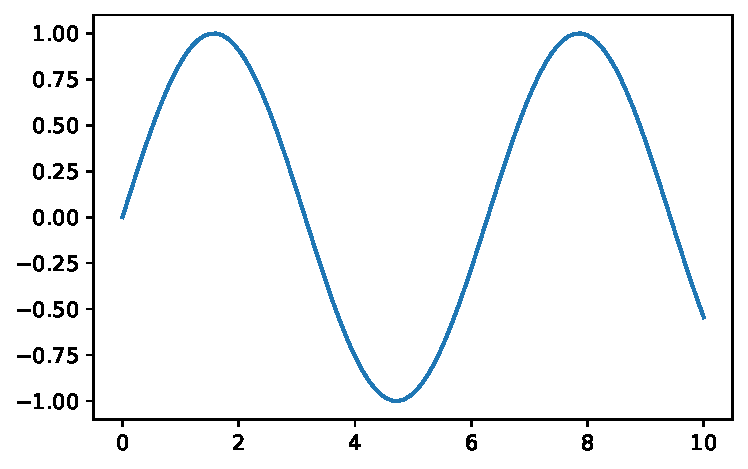
\includegraphics[keepaspectratio]{course/chapters/Plots/SimplePlots_files/figure-pdf/cell-3-output-1.pdf}}

To add more graphs to the same figure, use \texttt{plt.plot()} multiple
times before \texttt{plt.show()}. If you want to create a new figure,
use \texttt{plt.figure()} before \texttt{plt.plot()}.

\begin{Shaded}
\begin{Highlighting}[]
\NormalTok{plt.plot(x,y)}
\NormalTok{plt.plot(x,}\DecValTok{2}\OperatorTok{*}\NormalTok{y)}
\NormalTok{plt.show()}
\NormalTok{plt.plot(x, y)}
\NormalTok{plt.show()}
\end{Highlighting}
\end{Shaded}

\pandocbounded{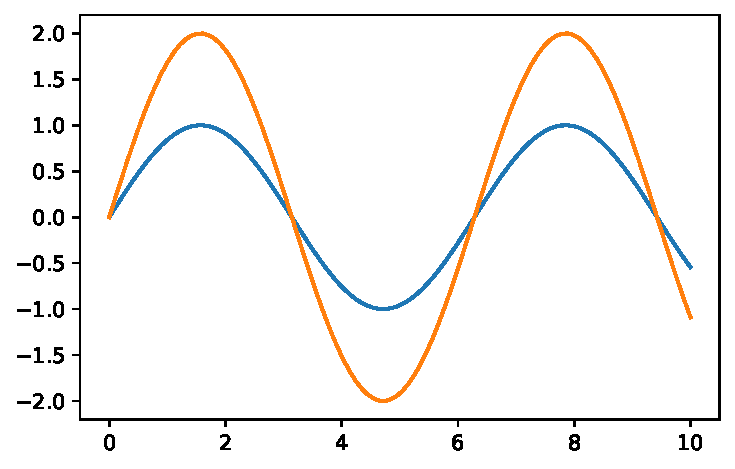
\includegraphics[keepaspectratio]{course/chapters/Plots/SimplePlots_files/figure-pdf/cell-4-output-1.pdf}}

\pandocbounded{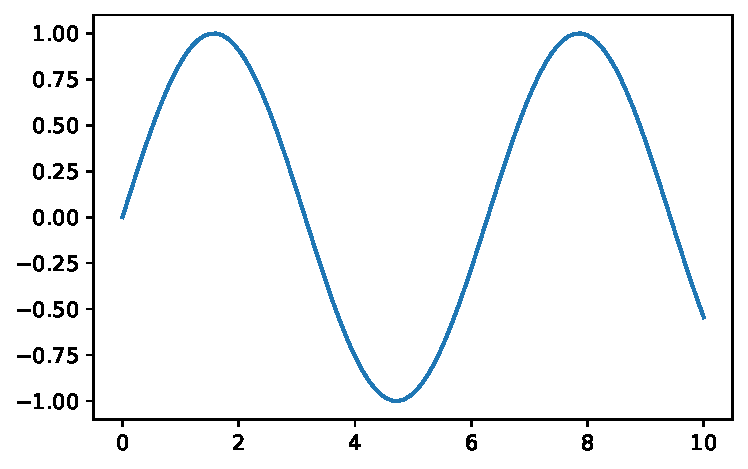
\includegraphics[keepaspectratio]{course/chapters/Plots/SimplePlots_files/figure-pdf/cell-4-output-2.pdf}}

\begin{center}\rule{0.5\linewidth}{0.5pt}\end{center}

\subsection*{3. Adjust the plot.}\label{adjust-the-plot.}
\addcontentsline{toc}{subsection}{3. Adjust the plot.}

The \texttt{plot()} function takes the following arguments:

\begin{itemize}
\tightlist
\item
  x-axis data points
\item
  y-axis data points
\item
  \href{https://matplotlib.org/stable/users/explain/colors/colors.html}{color}:
  hex, or color name (e.g., `red', `blue',`black'), abbreviated (e.g.,
  `r', `b',`k')
\item
  \href{https://matplotlib.org/stable/gallery/lines_bars_and_markers/linestyles.html}{linestyle}:
  `-', `--', `-.', `:' or ``solid'', ``dashed'', ``dashdot'', ``dotted''
\item
  \href{https://matplotlib.org/stable/api/markers_api.html}{marker}:
  `o', `x', `+', '*`, 's', `d', `\^{}', `v', `\textgreater{}',
  `\textless{}', `p', `h'
\item
  linewidth - width of the line
\item
  alpha - transparency of the line
\item
  markerfacecolor - color of the marker face
\item
  markersize - size of the marker
\item
  label - label for the data points
\end{itemize}

You have to call \texttt{plt.legend()} to show the labels.

\begin{Shaded}
\begin{Highlighting}[]
\NormalTok{plt.figure()}
\NormalTok{plt.plot(x, y, color}\OperatorTok{=}\StringTok{\textquotesingle{}red\textquotesingle{}}\NormalTok{, linestyle}\OperatorTok{=}\StringTok{\textquotesingle{}dashed\textquotesingle{}}\NormalTok{, linewidth}\OperatorTok{=}\DecValTok{2}\NormalTok{, marker}\OperatorTok{=}\StringTok{\textquotesingle{}o\textquotesingle{}}\NormalTok{, }
\NormalTok{            markerfacecolor}\OperatorTok{=}\StringTok{\textquotesingle{}blue\textquotesingle{}}\NormalTok{, markersize}\OperatorTok{=}\DecValTok{5}\NormalTok{,}
\NormalTok{            label}\OperatorTok{=}\StringTok{\textquotesingle{}sin(x)\textquotesingle{}}\NormalTok{)}
\NormalTok{plt.plot(x, }\DecValTok{2}\OperatorTok{*}\NormalTok{y, color}\OperatorTok{=}\StringTok{\textquotesingle{}darkgrey\textquotesingle{}}\NormalTok{, linestyle}\OperatorTok{=}\StringTok{\textquotesingle{}dotted\textquotesingle{}}\NormalTok{, linewidth}\OperatorTok{=}\DecValTok{2}\NormalTok{, marker}\OperatorTok{=}\StringTok{\textquotesingle{}x\textquotesingle{}}\NormalTok{,}
\NormalTok{            markerfacecolor}\OperatorTok{=}\StringTok{\textquotesingle{}grey\textquotesingle{}}\NormalTok{, markersize}\OperatorTok{=}\DecValTok{5}\NormalTok{,}
\NormalTok{            label}\OperatorTok{=}\StringTok{\textquotesingle{}2*sin(x)\textquotesingle{}}\NormalTok{)}
\NormalTok{plt.legend()}
\NormalTok{plt.show()}
\end{Highlighting}
\end{Shaded}

\pandocbounded{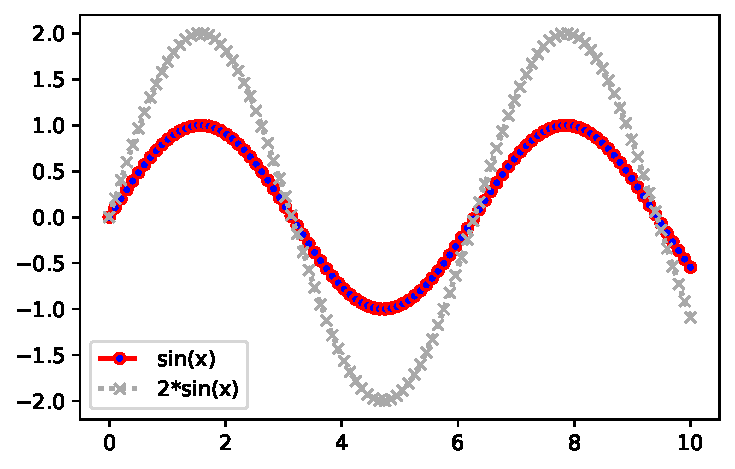
\includegraphics[keepaspectratio]{course/chapters/Plots/SimplePlots_files/figure-pdf/cell-5-output-1.pdf}}

\begin{center}\rule{0.5\linewidth}{0.5pt}\end{center}

\subsection*{4. Adust the figure}\label{adust-the-figure}
\addcontentsline{toc}{subsection}{4. Adust the figure}

This plot figure can be adjusted by changing the figure size, title,
labels, and so on.

\begin{itemize}
\tightlist
\item
  \texttt{plt.xlabel()}: Set the x-axis label of the current axis.
\item
  \texttt{plt.ylabel()}: Set the y-axis label of the current axis.
\item
  \texttt{plt.title()}: Set a title for the axes.
\item
  \texttt{plt.legend()}: Place a legend on the axes.
\item
  \texttt{plt.grid()}: Configure the grid lines.
\item
  \texttt{plt.xlim()}: Get or set the x-limits of the current axes.
\item
  \texttt{plt.ylim()}: Get or set the y-limits of the current axes.
\item
  \texttt{plt.xticks()}: Get or set the current tick locations and
  labels of the x-axis.
\item
  \texttt{plt.yticks()}: Get or set the current tick locations and
  labels of the y-axis.
\item
  \texttt{plt.figure()}: Create a new figure.
\item
  \texttt{plt.show()}: Display a figure.
\end{itemize}

\begin{Shaded}
\begin{Highlighting}[]
\NormalTok{plt.figure(figsize}\OperatorTok{=}\NormalTok{(}\DecValTok{4}\NormalTok{, }\DecValTok{4}\NormalTok{), dpi}\OperatorTok{=}\DecValTok{100}\NormalTok{)}
\CommentTok{\# Create a figure with a specific size and resolution}
\NormalTok{plt.plot(x, y, color}\OperatorTok{=}\StringTok{\textquotesingle{}red\textquotesingle{}}\NormalTok{, linestyle}\OperatorTok{=}\StringTok{\textquotesingle{}dashed\textquotesingle{}}\NormalTok{, linewidth}\OperatorTok{=}\DecValTok{2}\NormalTok{, marker}\OperatorTok{=}\StringTok{\textquotesingle{}o\textquotesingle{}}\NormalTok{, }
\NormalTok{            markerfacecolor}\OperatorTok{=}\StringTok{\textquotesingle{}blue\textquotesingle{}}\NormalTok{, markersize}\OperatorTok{=}\DecValTok{5}\NormalTok{,}
\NormalTok{            label}\OperatorTok{=}\StringTok{\textquotesingle{}sin(x)\textquotesingle{}}\NormalTok{)}
\NormalTok{plt.plot(x, }\DecValTok{2}\OperatorTok{*}\NormalTok{y, color}\OperatorTok{=}\StringTok{\textquotesingle{}darkgrey\textquotesingle{}}\NormalTok{, linestyle}\OperatorTok{=}\StringTok{\textquotesingle{}dotted\textquotesingle{}}\NormalTok{, linewidth}\OperatorTok{=}\DecValTok{2}\NormalTok{, marker}\OperatorTok{=}\StringTok{\textquotesingle{}x\textquotesingle{}}\NormalTok{,}
\NormalTok{            markerfacecolor}\OperatorTok{=}\StringTok{\textquotesingle{}grey\textquotesingle{}}\NormalTok{, markersize}\OperatorTok{=}\DecValTok{5}\NormalTok{,}
\NormalTok{            label}\OperatorTok{=}\StringTok{\textquotesingle{}2*sin(x)\textquotesingle{}}\NormalTok{)}
\NormalTok{plt.xlim([}\DecValTok{0}\NormalTok{, }\DecValTok{10}\NormalTok{]) }\CommentTok{\# set the x{-}axis limits}
\NormalTok{plt.ylim([}\OperatorTok{{-}}\DecValTok{3}\NormalTok{, }\DecValTok{3}\NormalTok{]) }\CommentTok{\# set the y{-}axis limits}
\NormalTok{plt.xticks(np.arange(}\DecValTok{0}\NormalTok{, }\DecValTok{11}\NormalTok{, }\DecValTok{2}\NormalTok{)) }\CommentTok{\# set the x{-}axis ticks}
\NormalTok{plt.yticks(np.arange(}\OperatorTok{{-}}\DecValTok{3}\NormalTok{, }\DecValTok{4}\NormalTok{, }\DecValTok{1}\NormalTok{)) }\CommentTok{\# set the y{-}axis ticks}
\NormalTok{plt.xlabel(}\StringTok{\textquotesingle{}x\textquotesingle{}}\NormalTok{) }\CommentTok{\# set the x{-}axis label}
\NormalTok{plt.ylabel(}\StringTok{\textquotesingle{}y\textquotesingle{}}\NormalTok{) }\CommentTok{\# set the y{-}axis label}
\NormalTok{plt.title(}\StringTok{\textquotesingle{}Sine and Double Sine Functions\textquotesingle{}}\NormalTok{) }\CommentTok{\# set the title of the plot}
\NormalTok{plt.grid(linewidth}\OperatorTok{=}\FloatTok{0.1}\NormalTok{)}\CommentTok{\# set the grid linewidth}
\NormalTok{plt.legend(loc}\OperatorTok{=}\StringTok{\textquotesingle{}upper left\textquotesingle{}}\NormalTok{) }\CommentTok{\# set the location of the legend: upper left, upper right, lower left, lower right}
\NormalTok{plt.show()}
\end{Highlighting}
\end{Shaded}

\pandocbounded{\includegraphics[keepaspectratio]{course/chapters/Plots/SimplePlots_files/figure-pdf/cell-6-output-1.pdf}}

\begin{center}\rule{0.5\linewidth}{0.5pt}\end{center}

\section*{Creating multiple plots}\label{creating-multiple-plots}
\addcontentsline{toc}{section}{Creating multiple plots}

\markright{Creating multiple plots}

You can create multiple plots in the same figure by using the
\texttt{subplot()} function.

\begin{Shaded}
\begin{Highlighting}[]
\NormalTok{plt.subplot(}\DecValTok{2}\NormalTok{, }\DecValTok{1}\NormalTok{, }\DecValTok{1}\NormalTok{)}
\NormalTok{plt.plot(x, y, color}\OperatorTok{=}\StringTok{\textquotesingle{}red\textquotesingle{}}\NormalTok{, linestyle}\OperatorTok{=}\StringTok{\textquotesingle{}dashed\textquotesingle{}}\NormalTok{, linewidth}\OperatorTok{=}\DecValTok{2}\NormalTok{, marker}\OperatorTok{=}\StringTok{\textquotesingle{}o\textquotesingle{}}\NormalTok{, }
\NormalTok{            markerfacecolor}\OperatorTok{=}\StringTok{\textquotesingle{}blue\textquotesingle{}}\NormalTok{, markersize}\OperatorTok{=}\DecValTok{5}\NormalTok{,}
\NormalTok{            label}\OperatorTok{=}\StringTok{\textquotesingle{}sin(x)\textquotesingle{}}\NormalTok{)}
\NormalTok{plt.xlabel(}\StringTok{\textquotesingle{}x\textquotesingle{}}\NormalTok{)}
\NormalTok{plt.ylabel(}\StringTok{\textquotesingle{}y\textquotesingle{}}\NormalTok{)}
\NormalTok{plt.title(}\StringTok{\textquotesingle{}Sine Function\textquotesingle{}}\NormalTok{)}
\NormalTok{plt.legend()}

\NormalTok{plt.subplot(}\DecValTok{2}\NormalTok{, }\DecValTok{1}\NormalTok{, }\DecValTok{2}\NormalTok{)}
\NormalTok{plt.plot(x, }\DecValTok{2}\OperatorTok{*}\NormalTok{y, color}\OperatorTok{=}\StringTok{\textquotesingle{}darkgrey\textquotesingle{}}\NormalTok{, linestyle}\OperatorTok{=}\StringTok{\textquotesingle{}dotted\textquotesingle{}}\NormalTok{, linewidth}\OperatorTok{=}\DecValTok{2}\NormalTok{, marker}\OperatorTok{=}\StringTok{\textquotesingle{}x\textquotesingle{}}\NormalTok{,}
\NormalTok{            markerfacecolor}\OperatorTok{=}\StringTok{\textquotesingle{}grey\textquotesingle{}}\NormalTok{, markersize}\OperatorTok{=}\DecValTok{5}\NormalTok{,}
\NormalTok{            label}\OperatorTok{=}\StringTok{\textquotesingle{}2*sin(x)\textquotesingle{}}\NormalTok{)}
\NormalTok{plt.xlabel(}\StringTok{\textquotesingle{}x\textquotesingle{}}\NormalTok{)}
\NormalTok{plt.ylabel(}\StringTok{\textquotesingle{}y\textquotesingle{}}\NormalTok{)}
\NormalTok{plt.title(}\StringTok{\textquotesingle{}Double Sine Function\textquotesingle{}}\NormalTok{)}
\NormalTok{plt.legend()   }
\NormalTok{plt.tight\_layout()}
\NormalTok{plt.show()}
\end{Highlighting}
\end{Shaded}

\pandocbounded{\includegraphics[keepaspectratio]{course/chapters/Plots/SimplePlots_files/figure-pdf/cell-7-output-1.pdf}}

\begin{Shaded}
\begin{Highlighting}[]
\NormalTok{fig }\OperatorTok{=}\NormalTok{ plt.figure(figsize}\OperatorTok{=}\NormalTok{(}\DecValTok{4}\NormalTok{,}\DecValTok{2}\NormalTok{),dpi}\OperatorTok{=}\DecValTok{72}\NormalTok{,layout}\OperatorTok{=}\StringTok{\textquotesingle{}constrained\textquotesingle{}}\NormalTok{, facecolor}\OperatorTok{=}\StringTok{\textquotesingle{}lightyellow\textquotesingle{}}\NormalTok{)}
\CommentTok{\# Create a figure with a specific layout and background color}
\CommentTok{\# constrained layout automatically adjusts the subplots to fit the figure}
\NormalTok{fig.suptitle(}\StringTok{\textquotesingle{}Figure\textquotesingle{}}\NormalTok{) }\CommentTok{\# set the title of the figure object}
\NormalTok{subL, subR }\OperatorTok{=}\NormalTok{ fig.subfigures(}\DecValTok{1}\NormalTok{, }\DecValTok{2}\NormalTok{) }\CommentTok{\# create two subfigures}
\NormalTok{subL.set\_facecolor(}\StringTok{\textquotesingle{}thistle\textquotesingle{}}\NormalTok{) }\CommentTok{\# set the background color of the left subfigure}
\NormalTok{sub\_subL }\OperatorTok{=}\NormalTok{ subL.subplots(}\DecValTok{2}\NormalTok{, }\DecValTok{1}\NormalTok{, sharex}\OperatorTok{=}\VariableTok{True}\NormalTok{) }\CommentTok{\# create two subplots in the left subfigure}
\NormalTok{sub\_subL[}\DecValTok{1}\NormalTok{].set\_xlabel(}\StringTok{\textquotesingle{}x [m]\textquotesingle{}}\NormalTok{)}
\NormalTok{subL.suptitle(}\StringTok{\textquotesingle{}Left subfigure\textquotesingle{}}\NormalTok{) }\CommentTok{\# set the title of the left subfigure}
\NormalTok{subR.set\_facecolor(}\StringTok{\textquotesingle{}lightskyblue\textquotesingle{}}\NormalTok{) }\CommentTok{\# set the background color of the right subfigure}
\NormalTok{sub\_subR }\OperatorTok{=}\NormalTok{ subR.subplots(}\DecValTok{1}\NormalTok{, }\DecValTok{2}\NormalTok{, sharey}\OperatorTok{=}\VariableTok{True}\NormalTok{) }
\NormalTok{sub\_subR[}\DecValTok{0}\NormalTok{].set\_title(}\StringTok{\textquotesingle{}Axes 1\textquotesingle{}}\NormalTok{) }\CommentTok{\# set the title of the first subplot in the right subfigure}
\NormalTok{sub\_subR[}\DecValTok{1}\NormalTok{].set\_title(}\StringTok{\textquotesingle{}Axes 2\textquotesingle{}}\NormalTok{) }\CommentTok{\# set the title of the second subplot in the right subfigure}
\NormalTok{subR.suptitle(}\StringTok{\textquotesingle{}Right subfigure\textquotesingle{}}\NormalTok{)}
\end{Highlighting}
\end{Shaded}

\begin{verbatim}
Text(0.5, 0.98, 'Right subfigure')
\end{verbatim}

\pandocbounded{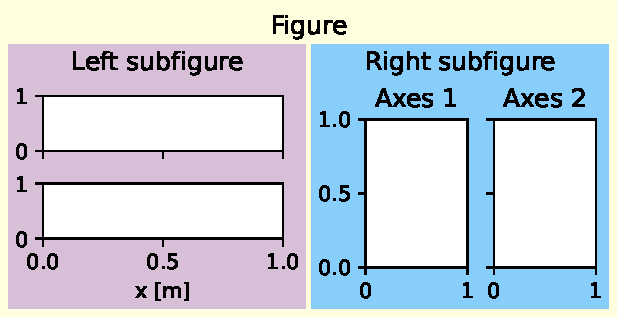
\includegraphics[keepaspectratio]{course/chapters/Plots/SimplePlots_files/figure-pdf/cell-8-output-2.pdf}}

\subsection{Subfigures and Gridspec}\label{subfigures-and-gridspec}

You can also create \texttt{subplots} and \texttt{gridspecs} to create
more complex layouts.

\begin{Shaded}
\begin{Highlighting}[]
\ImportTok{from}\NormalTok{ matplotlib.gridspec }\ImportTok{import}\NormalTok{ GridSpec}
\ImportTok{from}\NormalTok{ matplotlib }\ImportTok{import}\NormalTok{ pyplot }\ImportTok{as}\NormalTok{ plt}
\ImportTok{import}\NormalTok{ numpy }\ImportTok{as}\NormalTok{ np}
\end{Highlighting}
\end{Shaded}

\begin{Shaded}
\begin{Highlighting}[]
\NormalTok{x }\OperatorTok{=}\NormalTok{ np.linspace(}\DecValTok{0}\NormalTok{, }\DecValTok{10}\NormalTok{, }\DecValTok{100}\NormalTok{)}
\NormalTok{y }\OperatorTok{=}\NormalTok{ np.sin(x)}

\NormalTok{fig, ax }\OperatorTok{=}\NormalTok{ plt.subplots(}\DecValTok{3}\NormalTok{,}\DecValTok{2}\NormalTok{, figsize}\OperatorTok{=}\NormalTok{(}\DecValTok{3}\NormalTok{,}\DecValTok{4}\NormalTok{), dpi}\OperatorTok{=}\DecValTok{96}\NormalTok{, sharex}\OperatorTok{=}\VariableTok{True}\NormalTok{, sharey}\OperatorTok{=}\VariableTok{True}\NormalTok{, constrained\_layout}\OperatorTok{=}\VariableTok{True}\NormalTok{,gridspec\_kw}\OperatorTok{=}\NormalTok{\{}\StringTok{\textquotesingle{}hspace\textquotesingle{}}\NormalTok{: }\FloatTok{0.2}\NormalTok{, }\StringTok{\textquotesingle{}wspace\textquotesingle{}}\NormalTok{: }\FloatTok{0.2}\NormalTok{\})}

\ControlFlowTok{for}\NormalTok{ i }\KeywordTok{in} \BuiltInTok{range}\NormalTok{(}\DecValTok{3}\NormalTok{):}
    \ControlFlowTok{for}\NormalTok{ j }\KeywordTok{in} \BuiltInTok{range}\NormalTok{(}\DecValTok{2}\NormalTok{):}
\NormalTok{        ax[i,j].plot(x, y}\OperatorTok{*}\NormalTok{(i}\OperatorTok{+}\DecValTok{1}\NormalTok{)}\OperatorTok{*}\NormalTok{(j}\OperatorTok{+}\DecValTok{1}\NormalTok{))}

\NormalTok{plt.show()}
\end{Highlighting}
\end{Shaded}

\pandocbounded{\includegraphics[keepaspectratio]{course/chapters/Plots/SimplePlots_files/figure-pdf/cell-10-output-1.pdf}}

\begin{Shaded}
\begin{Highlighting}[]
\NormalTok{x }\OperatorTok{=}\NormalTok{ np.linspace(}\DecValTok{0}\NormalTok{, }\DecValTok{10}\NormalTok{, }\DecValTok{100}\NormalTok{)}
\NormalTok{y }\OperatorTok{=}\NormalTok{ np.sin(x)}

\NormalTok{fig }\OperatorTok{=}\NormalTok{ plt.figure(figsize}\OperatorTok{=}\NormalTok{(}\DecValTok{4}\NormalTok{, }\DecValTok{6}\NormalTok{), dpi}\OperatorTok{=}\DecValTok{100}\NormalTok{)}
\NormalTok{gs }\OperatorTok{=}\NormalTok{ GridSpec(}\DecValTok{3}\NormalTok{, }\DecValTok{2}\NormalTok{, figure}\OperatorTok{=}\NormalTok{fig, hspace}\OperatorTok{=}\FloatTok{0.4}\NormalTok{, wspace}\OperatorTok{=}\FloatTok{0.3}\NormalTok{)}

\ControlFlowTok{for}\NormalTok{ i }\KeywordTok{in} \BuiltInTok{range}\NormalTok{(}\DecValTok{3}\NormalTok{):}
    \ControlFlowTok{for}\NormalTok{ j }\KeywordTok{in} \BuiltInTok{range}\NormalTok{(}\DecValTok{2}\NormalTok{):}
\NormalTok{        ax }\OperatorTok{=}\NormalTok{ fig.add\_subplot(gs[i, j])}
\NormalTok{        ax.plot(x, y}\OperatorTok{*}\NormalTok{(i}\OperatorTok{+}\DecValTok{1}\NormalTok{)}\OperatorTok{*}\NormalTok{(j}\OperatorTok{+}\DecValTok{1}\NormalTok{))}
\NormalTok{        ax.set\_title(}\SpecialStringTok{f\textquotesingle{}Plot }\SpecialCharTok{\{}\NormalTok{i}\OperatorTok{+}\DecValTok{1}\SpecialCharTok{\}}\SpecialStringTok{, }\SpecialCharTok{\{}\NormalTok{j}\OperatorTok{+}\DecValTok{1}\SpecialCharTok{\}}\SpecialStringTok{\textquotesingle{}}\NormalTok{)}

\NormalTok{plt.show()}
\end{Highlighting}
\end{Shaded}

\pandocbounded{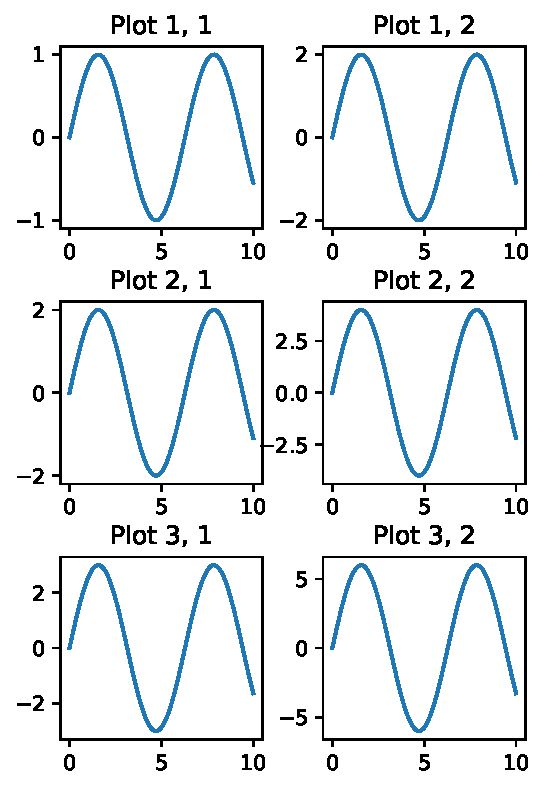
\includegraphics[keepaspectratio]{course/chapters/Plots/SimplePlots_files/figure-pdf/cell-11-output-1.pdf}}

\subsection*{Exercises}\label{exercises-2}
\addcontentsline{toc}{subsection}{Exercises}

Download it locally and try to solve the exercises.

\href{https://github.com/stkroe/PythonforChemists/blob/main/course/examples/SimplePlotExmple.ipynb}{Simple
Plot Example}

Or open it in \texttt{Google\ Colab}:

\href{https://colab.research.google.com/github/stkroe/PythonforChemists/blob/main/course/examples/SimplePlotExample.ipynb}{Simple
Plot Example}

\chapter{Simple Plot Types}\label{simple-plot-types}

Difficulty level: { }

\section*{Types of Plots}\label{types-of-plots}
\addcontentsline{toc}{section}{Types of Plots}

\markright{Types of Plots}

There exists are lot of different visualization techniques.

How you should visualize the data depends on the data and the question
you want to answer.

\begin{itemize}
\item
  \textbf{Distributions} can be visualized with a boxplot, a
  \emph{violinplot}, a \emph{histogram} or a \emph{density plot}.
\item
  \textbf{Relationships} between two variables can be visualized with a
  \emph{scatterplot}, a \emph{lineplot}, a \emph{regplot} or a
  \emph{jointplot}.
\item
  \textbf{Descriptions} of the data can be visualized with a
  \emph{barplot}, \emph{network plot} or a \emph{pie chart}.
\end{itemize}

\section{Relationship plots}\label{relationship-plots}

\subsection{Scatter Plot}\label{scatter-plot}

\href{https://matplotlib.org/stable/api/_as_gen/matplotlib.pyplot.scatter.html}{Scatter
plot} shows the relationship of observable over the abscissa \emph{e.g.}
time vs temperature as \textbf{discrete} function.

The \texttt{scatter()} function creates a scatter plot.

\begin{Shaded}
\begin{Highlighting}[]
\NormalTok{plt.scatter()}
\end{Highlighting}
\end{Shaded}

\begin{tcolorbox}[enhanced jigsaw, leftrule=.75mm, bottomrule=.15mm, colbacktitle=quarto-callout-note-color!10!white, title=\textcolor{quarto-callout-note-color}{\faInfo}\hspace{0.5em}{Note}, breakable, arc=.35mm, toptitle=1mm, opacityback=0, titlerule=0mm, coltitle=black, colback=white, opacitybacktitle=0.6, colframe=quarto-callout-note-color-frame, left=2mm, rightrule=.15mm, toprule=.15mm, bottomtitle=1mm]

The marker size can be adjusted with the \texttt{s} parameter.

\end{tcolorbox}

\begin{Shaded}
\begin{Highlighting}[]
\ImportTok{import}\NormalTok{ matplotlib.pyplot }\ImportTok{as}\NormalTok{ plt}
\ImportTok{import}\NormalTok{ numpy }\ImportTok{as}\NormalTok{ np}

\NormalTok{x }\OperatorTok{=}\NormalTok{ np.linspace(}\DecValTok{0}\NormalTok{, }\DecValTok{10}\NormalTok{, }\DecValTok{100}\NormalTok{)}
\NormalTok{y }\OperatorTok{=}\NormalTok{ np.random.rand(}\DecValTok{100}\NormalTok{)}\OperatorTok{*}\NormalTok{np.sin(x)}

\NormalTok{plt.scatter(x, y, color}\OperatorTok{=}\StringTok{\textquotesingle{}grey\textquotesingle{}}\NormalTok{, marker}\OperatorTok{=}\StringTok{\textquotesingle{}o\textquotesingle{}}\NormalTok{, label}\OperatorTok{=}\StringTok{\textquotesingle{}sin(x)\textquotesingle{}}\NormalTok{,s}\OperatorTok{=}\DecValTok{5}\NormalTok{)}
\NormalTok{plt.xlabel(}\StringTok{\textquotesingle{}x\textquotesingle{}}\NormalTok{)}
\NormalTok{plt.ylabel(}\StringTok{\textquotesingle{}y\textquotesingle{}}\NormalTok{)}
\NormalTok{plt.legend()}
\NormalTok{plt.show()}
\end{Highlighting}
\end{Shaded}

\pandocbounded{\includegraphics[keepaspectratio]{course/chapters/Plots/SimplePlotTypes_files/figure-pdf/cell-3-output-1.pdf}}

\subsection{Line Plot}\label{line-plot}

\href{https://matplotlib.org/stable/api/_as_gen/matplotlib.pyplot.plot.html}{Line
plot} shows the relationship of observable over the abscissa \emph{e.g.}
time vs radioactivity decay as \textbf{continuous} function.

The \texttt{plot()} function creates a line plot but can also be used to
create scatter plots.

\begin{tcolorbox}[enhanced jigsaw, leftrule=.75mm, bottomrule=.15mm, colbacktitle=quarto-callout-note-color!10!white, title=\textcolor{quarto-callout-note-color}{\faInfo}\hspace{0.5em}{Note}, breakable, arc=.35mm, toptitle=1mm, opacityback=0, titlerule=0mm, coltitle=black, colback=white, opacitybacktitle=0.6, colframe=quarto-callout-note-color-frame, left=2mm, rightrule=.15mm, toprule=.15mm, bottomtitle=1mm]

The marker size can be adjusted with the \texttt{markersize} parameter.

\end{tcolorbox}

\begin{Shaded}
\begin{Highlighting}[]
\ImportTok{import}\NormalTok{ matplotlib.pyplot }\ImportTok{as}\NormalTok{ plt}
\ImportTok{import}\NormalTok{ numpy }\ImportTok{as}\NormalTok{ np}

\NormalTok{x }\OperatorTok{=}\NormalTok{ np.linspace(}\DecValTok{0}\NormalTok{, }\DecValTok{10}\NormalTok{, }\DecValTok{100}\NormalTok{)}
\NormalTok{y }\OperatorTok{=}\NormalTok{ np.random.rand(}\DecValTok{100}\NormalTok{)}\OperatorTok{+}\NormalTok{np.sin(x)}

\NormalTok{plt.plot(x, y, color}\OperatorTok{=}\StringTok{\textquotesingle{}grey\textquotesingle{}}\NormalTok{, marker}\OperatorTok{=}\StringTok{\textquotesingle{}o\textquotesingle{}}\NormalTok{, label}\OperatorTok{=}\StringTok{\textquotesingle{}sin(x)\textquotesingle{}}\NormalTok{,markersize}\OperatorTok{=}\DecValTok{5}\NormalTok{,linewidth}\OperatorTok{=}\DecValTok{2}\NormalTok{,linestyle}\OperatorTok{=}\StringTok{\textquotesingle{}{-}{-}\textquotesingle{}}\NormalTok{)}
\NormalTok{plt.xlabel(}\StringTok{\textquotesingle{}x\textquotesingle{}}\NormalTok{)}
\NormalTok{plt.ylabel(}\StringTok{\textquotesingle{}y\textquotesingle{}}\NormalTok{)}
\NormalTok{plt.legend()}
\NormalTok{plt.show()}
\end{Highlighting}
\end{Shaded}

\pandocbounded{\includegraphics[keepaspectratio]{course/chapters/Plots/SimplePlotTypes_files/figure-pdf/cell-4-output-1.pdf}}

\subsection{Errorbars}\label{errorbars}

\href{https://matplotlib.org/stable/api/_as_gen/matplotlib.axes.Axes.errorbar.html\#matplotlib.axes.Axes.errorbar}{Errorbars}
can be added to the plot with the \texttt{errorbar()} function and the
\texttt{yerr} parameter.

\begin{Shaded}
\begin{Highlighting}[]
\ImportTok{import}\NormalTok{ matplotlib.pyplot }\ImportTok{as}\NormalTok{ plt}
\ImportTok{import}\NormalTok{ numpy }\ImportTok{as}\NormalTok{ np}

\NormalTok{x }\OperatorTok{=}\NormalTok{ np.linspace(}\DecValTok{0}\NormalTok{, }\DecValTok{10}\NormalTok{, }\DecValTok{100}\NormalTok{)}
\NormalTok{y }\OperatorTok{=}\NormalTok{ np.random.rand(}\DecValTok{100}\NormalTok{)}\OperatorTok{*}\DecValTok{298}
\NormalTok{yerr }\OperatorTok{=}\NormalTok{ np.random.rand(}\DecValTok{100}\NormalTok{)}\OperatorTok{*}\DecValTok{10}

\NormalTok{plt.errorbar(x, y, yerr}\OperatorTok{=}\NormalTok{yerr, color}\OperatorTok{=}\StringTok{\textquotesingle{}grey\textquotesingle{}}\NormalTok{, marker}\OperatorTok{=}\StringTok{\textquotesingle{}o\textquotesingle{}}\NormalTok{, label}\OperatorTok{=}\StringTok{\textquotesingle{}sin(x)\textquotesingle{}}\NormalTok{,markersize}\OperatorTok{=}\DecValTok{5}\NormalTok{,linewidth}\OperatorTok{=}\DecValTok{2}\NormalTok{,elinewidth}\OperatorTok{=}\DecValTok{3}\NormalTok{,errorevery}\OperatorTok{=}\NormalTok{(}\DecValTok{10}\NormalTok{, }\DecValTok{3}\NormalTok{), capsize}\OperatorTok{=}\DecValTok{5}\NormalTok{, ecolor}\OperatorTok{=}\StringTok{\textquotesingle{}black\textquotesingle{}}\NormalTok{)}
\NormalTok{plt.xlabel(}\StringTok{\textquotesingle{}x\textquotesingle{}}\NormalTok{)}
\NormalTok{plt.ylabel(}\StringTok{\textquotesingle{}y\textquotesingle{}}\NormalTok{)}
\NormalTok{plt.legend()}
\NormalTok{plt.show()}
\end{Highlighting}
\end{Shaded}

\pandocbounded{\includegraphics[keepaspectratio]{course/chapters/Plots/SimplePlotTypes_files/figure-pdf/cell-5-output-1.pdf}}

\begin{itemize}
\tightlist
\item
  The \texttt{yerr} parameter can be used to set the error bars for the
  y-axis.
\item
  The \texttt{xerr} parameter can be used to set the error bars for the
  x-axis.
\item
  The parameter \texttt{errorevery} can be used to show only every 3th
  error bar - starting from the 10th error bar.
\item
  The \texttt{capsize} parameter can be used to set the size of the
  error bar caps.
\item
  The \texttt{elinewidth} parameter can be used to set the width of the
  error bar line.
\item
  The \texttt{ecolor} parameter can be used to set the color of the
  error bar line.
\end{itemize}

\begin{center}\rule{0.5\linewidth}{0.5pt}\end{center}

\section{Distribution Plots}\label{distribution-plots}

\subsection*{Histogram Plot}\label{histogram-plot}
\addcontentsline{toc}{subsection}{Histogram Plot}

{[}Histogram{]}
(https://matplotlib.org/stable/api/\_as\_gen/matplotlib.pyplot.hist.html)
shows the distribution of a single variable \emph{e.g.} count of a mass
of individuals in a population. The data is divided into bins and the
number of data points in each bin is plotted.

The histogram visualizes the skewness, kurtosis and outliers of the
data.

The \texttt{hist()} function creates a histogram with \texttt{bins}
number of bins.

\begin{Shaded}
\begin{Highlighting}[]
\ImportTok{import}\NormalTok{ matplotlib.pyplot }\ImportTok{as}\NormalTok{ plt}
\ImportTok{import}\NormalTok{ numpy }\ImportTok{as}\NormalTok{ np}

\NormalTok{x }\OperatorTok{=}\NormalTok{ np.random.randn(}\DecValTok{1000}\NormalTok{)}

\NormalTok{plt.hist(x, bins}\OperatorTok{=}\DecValTok{30}\NormalTok{, color}\OperatorTok{=}\StringTok{\textquotesingle{}grey\textquotesingle{}}\NormalTok{, edgecolor}\OperatorTok{=}\StringTok{\textquotesingle{}black\textquotesingle{}}\NormalTok{)}

\NormalTok{plt.xlabel(}\StringTok{\textquotesingle{}x\textquotesingle{}}\NormalTok{)}
\NormalTok{plt.ylabel(}\StringTok{\textquotesingle{}y\textquotesingle{}}\NormalTok{)}
\NormalTok{plt.show()}
\end{Highlighting}
\end{Shaded}

\pandocbounded{\includegraphics[keepaspectratio]{course/chapters/Plots/SimplePlotTypes_files/figure-pdf/cell-6-output-1.pdf}}

\href{https://matplotlib.org/stable/api/_as_gen/matplotlib.axes.Axes.hist2d.html\#matplotlib.axes.Axes.hist2d}{2D
histograms} can be created with the \texttt{hist2d()} function.

\begin{Shaded}
\begin{Highlighting}[]
\ImportTok{import}\NormalTok{ matplotlib.pyplot }\ImportTok{as}\NormalTok{ plt}
\ImportTok{import}\NormalTok{ numpy }\ImportTok{as}\NormalTok{ np}

\NormalTok{x }\OperatorTok{=}\NormalTok{ np.random.randn(}\DecValTok{1000}\NormalTok{)}
\NormalTok{y }\OperatorTok{=}\NormalTok{ np.random.randn(}\DecValTok{1000}\NormalTok{)}
\NormalTok{plt.hist2d(x, y, bins}\OperatorTok{=}\DecValTok{30}\NormalTok{, cmap}\OperatorTok{=}\StringTok{\textquotesingle{}Greys\textquotesingle{}}\NormalTok{)}
\NormalTok{plt.colorbar()}
\NormalTok{plt.xlabel(}\StringTok{\textquotesingle{}x\textquotesingle{}}\NormalTok{)}
\NormalTok{plt.ylabel(}\StringTok{\textquotesingle{}y\textquotesingle{}}\NormalTok{)}
\NormalTok{plt.show()}
\end{Highlighting}
\end{Shaded}

\pandocbounded{\includegraphics[keepaspectratio]{course/chapters/Plots/SimplePlotTypes_files/figure-pdf/cell-7-output-1.pdf}}

\begin{itemize}
\tightlist
\item
  The \texttt{cmap} parameter is used to set the color map of the
  histogram.
\item
  The \texttt{colorbar()} function adds a color bar to the plot.
\end{itemize}

\subsection*{Boxplot}\label{boxplot}
\addcontentsline{toc}{subsection}{Boxplot}

\href{https://matplotlib.org/stable/api/_as_gen/matplotlib.pyplot.boxplot.html}{Box
plot} shows the distribution of a numerical variable for different
categories. It shows the minimum, first quartile, median, third quartile
and maximum of your data. Outliers can be identified. An example of this
\emph{e.g.} is the distribution of cancer cell survival time for
different treatment groups.

The \texttt{boxplot()} function creates a boxplot.

\begin{Shaded}
\begin{Highlighting}[]
\ImportTok{import}\NormalTok{ matplotlib.pyplot }\ImportTok{as}\NormalTok{ plt}
\ImportTok{import}\NormalTok{ numpy }\ImportTok{as}\NormalTok{ np}

\NormalTok{std }\OperatorTok{=} \DecValTok{2}
\NormalTok{data }\OperatorTok{=}\NormalTok{ [np.random.normal(}\DecValTok{0}\NormalTok{, std, }\DecValTok{100}\NormalTok{) }\ControlFlowTok{for}\NormalTok{ std }\KeywordTok{in} \BuiltInTok{range}\NormalTok{(}\DecValTok{1}\NormalTok{, }\DecValTok{4}\NormalTok{)]}


\NormalTok{plt.boxplot(data, patch\_artist}\OperatorTok{=}\VariableTok{True}\NormalTok{, notch}\OperatorTok{=}\VariableTok{True}\NormalTok{, showmeans}\OperatorTok{=}\VariableTok{True}\NormalTok{, meanline}\OperatorTok{=}\VariableTok{True}\NormalTok{, showfliers}\OperatorTok{=}\VariableTok{True}\NormalTok{, showbox}\OperatorTok{=}\VariableTok{True}\NormalTok{, showcaps}\OperatorTok{=}\VariableTok{True}\NormalTok{, orientation}\OperatorTok{=}\StringTok{\textquotesingle{}horizontal\textquotesingle{}}\NormalTok{,sym}\OperatorTok{=}\StringTok{\textquotesingle{}C0+\textquotesingle{}}\NormalTok{,}
\NormalTok{            boxprops}\OperatorTok{=}\BuiltInTok{dict}\NormalTok{(facecolor}\OperatorTok{=}\StringTok{\textquotesingle{}darkgrey\textquotesingle{}}\NormalTok{, color}\OperatorTok{=}\StringTok{\textquotesingle{}black\textquotesingle{}}\NormalTok{),}
\NormalTok{            medianprops}\OperatorTok{=}\BuiltInTok{dict}\NormalTok{(color}\OperatorTok{=}\StringTok{\textquotesingle{}grey\textquotesingle{}}\NormalTok{),}
\NormalTok{            whiskerprops}\OperatorTok{=}\BuiltInTok{dict}\NormalTok{(color}\OperatorTok{=}\StringTok{\textquotesingle{}black\textquotesingle{}}\NormalTok{),}
\NormalTok{            capprops}\OperatorTok{=}\BuiltInTok{dict}\NormalTok{(color}\OperatorTok{=}\StringTok{\textquotesingle{}black\textquotesingle{}}\NormalTok{),}
\NormalTok{            meanprops}\OperatorTok{=}\BuiltInTok{dict}\NormalTok{(color}\OperatorTok{=}\StringTok{\textquotesingle{}black\textquotesingle{}}\NormalTok{, linewidth}\OperatorTok{=}\DecValTok{2}\NormalTok{))}
\NormalTok{plt.yticks([}\DecValTok{1}\NormalTok{, }\DecValTok{2}\NormalTok{, }\DecValTok{3}\NormalTok{], [}\StringTok{\textquotesingle{}A\textquotesingle{}}\NormalTok{, }\StringTok{\textquotesingle{}B\textquotesingle{}}\NormalTok{, }\StringTok{\textquotesingle{}C\textquotesingle{}}\NormalTok{])}
\NormalTok{plt.title(}\StringTok{\textquotesingle{}Boxplot\textquotesingle{}}\NormalTok{)}
\NormalTok{plt.xlabel(}\StringTok{\textquotesingle{}x\textquotesingle{}}\NormalTok{)}
\NormalTok{plt.ylabel(}\StringTok{\textquotesingle{}y\textquotesingle{}}\NormalTok{)}
\NormalTok{plt.show()}
\end{Highlighting}
\end{Shaded}

\pandocbounded{\includegraphics[keepaspectratio]{course/chapters/Plots/SimplePlotTypes_files/figure-pdf/cell-8-output-1.pdf}}

\begin{itemize}
\tightlist
\item
  The \texttt{patch\_artist} parameter is used to fill the box with
  color.
\item
  The \texttt{notch} parameter is used to create a notch in the box.
\item
  The \texttt{showmeans} parameter is used to show the mean of the data.
\item
  The \texttt{meanline} parameter is used to show the mean line.
\item
  The \texttt{showfliers} parameter is used to show the outliers of the
  data.
\item
  The \texttt{showbox} parameter is used to show the box of the data.
\item
  The \texttt{showcaps} parameter is used to show the caps of the data.
\item
  The \texttt{orientation} parameter is used to set the orientation of
  the boxplot. The default is \texttt{vertical}. If you want to create a
  horizontal boxplot, set it to \texttt{horizontal}.
\item
  The \texttt{sym} parameter is used to set the symbol of the outliers.
  The default is \texttt{o}. If you want to use a different symbol, set
  it to \texttt{r+} or any other symbol you want to use.
\item
  The \texttt{boxprops} parameter is used to set the properties of the
  box. The \texttt{facecolor} parameter is used to set the color of the
  box. The \texttt{color} parameter is used to set the color of the box
  outline.
\item
  The \texttt{medianprops} parameter is used to set the properties of
  the median line. The \texttt{color} parameter is used to set the color
  of the median line.
\item
  The \texttt{whiskerprops} parameter is used to set the properties of
  the whiskers. The \texttt{color} parameter is used to set the color of
  the whiskers.
\item
  The \texttt{meanprops} parameter is used to set the properties of the
  mean line. The \texttt{color} parameter is used to set the color of
  the mean line.
\item
  The \texttt{capprops} parameter is used to set the properties of the
  caps. The \texttt{color} parameter is used to set the color of the
  caps.
\end{itemize}

\subsection*{Proportion Plots}\label{proportion-plots}
\addcontentsline{toc}{subsection}{Proportion Plots}

\section*{Bar Plot}\label{bar-plot}
\addcontentsline{toc}{section}{Bar Plot}

\markright{Bar Plot}

\href{https://matplotlib.org/stable/api/_as_gen/matplotlib.pyplot.bar.html}{Bar
plot} shows the relationship of a categorical variable with a numerical
variable \emph{e.g.} cancer cell survival time for different treatment
groups. The height of the bar is proportional to the value of the
investigated variable.

The \texttt{bar()} function creates a bar plot.

\begin{Shaded}
\begin{Highlighting}[]
\ImportTok{import}\NormalTok{ matplotlib.pyplot }\ImportTok{as}\NormalTok{ plt}
\ImportTok{import}\NormalTok{ numpy }\ImportTok{as}\NormalTok{ np}
\ImportTok{import}\NormalTok{ scipy.stats }\ImportTok{as}\NormalTok{ stats}

\NormalTok{x }\OperatorTok{=}\NormalTok{ [}\StringTok{\textquotesingle{}A\textquotesingle{}}\NormalTok{, }\StringTok{\textquotesingle{}B\textquotesingle{}}\NormalTok{, }\StringTok{\textquotesingle{}C\textquotesingle{}}\NormalTok{, }\StringTok{\textquotesingle{}D\textquotesingle{}}\NormalTok{]}
\NormalTok{y }\OperatorTok{=}\NormalTok{ [}\DecValTok{10}\NormalTok{, }\DecValTok{20}\NormalTok{, }\DecValTok{30}\NormalTok{, }\DecValTok{40}\NormalTok{]}
\NormalTok{yerr }\OperatorTok{=}\NormalTok{ np.random.rand(}\DecValTok{4}\NormalTok{)}\OperatorTok{*}\DecValTok{10}

\NormalTok{plt.bar(x, y,yerr}\OperatorTok{=}\NormalTok{yerr, color}\OperatorTok{=}\StringTok{\textquotesingle{}grey\textquotesingle{}}\NormalTok{)}

\NormalTok{plt.xlabel(}\StringTok{\textquotesingle{}x\textquotesingle{}}\NormalTok{)}
\NormalTok{plt.ylabel(}\StringTok{\textquotesingle{}y\textquotesingle{}}\NormalTok{)}
\NormalTok{plt.show()}
\end{Highlighting}
\end{Shaded}

\pandocbounded{\includegraphics[keepaspectratio]{course/chapters/Plots/SimplePlotTypes_files/figure-pdf/cell-9-output-1.pdf}}

You can draw a star sign to indicate the significance of the data.

\section*{Pie Chart}\label{pie-chart}
\addcontentsline{toc}{section}{Pie Chart}

\markright{Pie Chart}

\href{https://matplotlib.org/stable/api/_as_gen/matplotlib.pyplot.pie.html}{Pie
chart} show the proportion of different categories in a single variable
\emph{e.g.} the content of different amino acids in a protein.

The \texttt{pie()} function creates a pie chart.

\begin{Shaded}
\begin{Highlighting}[]
\ImportTok{import}\NormalTok{ matplotlib.pyplot }\ImportTok{as}\NormalTok{ plt}
\ImportTok{import}\NormalTok{ numpy }\ImportTok{as}\NormalTok{ np}

\NormalTok{x }\OperatorTok{=}\NormalTok{ [}\DecValTok{10}\NormalTok{, }\DecValTok{20}\NormalTok{, }\DecValTok{30}\NormalTok{, }\DecValTok{40}\NormalTok{]}
\NormalTok{labels }\OperatorTok{=}\NormalTok{ [}\StringTok{\textquotesingle{}A\textquotesingle{}}\NormalTok{, }\StringTok{\textquotesingle{}B\textquotesingle{}}\NormalTok{, }\StringTok{\textquotesingle{}C\textquotesingle{}}\NormalTok{, }\StringTok{\textquotesingle{}D\textquotesingle{}}\NormalTok{]}

\NormalTok{plt.pie(x, labels}\OperatorTok{=}\NormalTok{labels, autopct}\OperatorTok{=}\StringTok{\textquotesingle{}}\SpecialCharTok{\%1.1f\%\%}\StringTok{\textquotesingle{}}\NormalTok{, startangle}\OperatorTok{=}\DecValTok{90}\NormalTok{, colors}\OperatorTok{=}\NormalTok{[}\StringTok{\textquotesingle{}lightgrey\textquotesingle{}}\NormalTok{, }\StringTok{\textquotesingle{}grey\textquotesingle{}}\NormalTok{, }\StringTok{\textquotesingle{}darkgrey\textquotesingle{}}\NormalTok{, }\StringTok{\textquotesingle{}dimgrey\textquotesingle{}}\NormalTok{], explode}\OperatorTok{=}\NormalTok{(}\FloatTok{0.1}\NormalTok{, }\DecValTok{0}\NormalTok{, }\DecValTok{0}\NormalTok{, }\DecValTok{0}\NormalTok{), shadow}\OperatorTok{=}\VariableTok{True}\NormalTok{)}
\NormalTok{plt.axis(}\StringTok{\textquotesingle{}equal\textquotesingle{}}\NormalTok{)  }\CommentTok{\# Equal aspect ratio ensures that pie is drawn as a circle.}

\NormalTok{plt.show()}
\end{Highlighting}
\end{Shaded}

\pandocbounded{\includegraphics[keepaspectratio]{course/chapters/Plots/SimplePlotTypes_files/figure-pdf/cell-10-output-1.pdf}}

\chapter{Seaborn Plots}\label{seaborn-plots}

Difficulty level: { }

\section*{Plotting with Seaborn}\label{plotting-with-seaborn}
\addcontentsline{toc}{section}{Plotting with Seaborn}

\markright{Plotting with Seaborn}

Seaborn is a Python data visualization library based on Matplotlib. It
provides a high-level interface for drawing attractive and informative
statistical graphics. Seaborn is built on top of Matplotlib and closely
integrated with pandas data structures.

\subsection*{KDE Plot}\label{kde-plot}
\addcontentsline{toc}{subsection}{KDE Plot}

\href{https://seaborn.pydata.org/generated/seaborn.kdeplot.html}{Kernel
density plot} show the distribution of a single variable \emph{e.g.}
distribution of a mass of individuals in a population. The data is
smoothed by a kernel density and the density of the data is plotted
continuously.

\begin{Shaded}
\begin{Highlighting}[]
\ImportTok{import}\NormalTok{ seaborn }\ImportTok{as}\NormalTok{ sns}
\ImportTok{import}\NormalTok{ matplotlib.pyplot }\ImportTok{as}\NormalTok{ plt}
\ImportTok{import}\NormalTok{ numpy }\ImportTok{as}\NormalTok{ np}
\ImportTok{import}\NormalTok{ pandas }\ImportTok{as}\NormalTok{ pd}

\CommentTok{\# Create a dataset}
\NormalTok{data }\OperatorTok{=}\NormalTok{ np.random.normal(loc}\OperatorTok{=}\DecValTok{0}\NormalTok{, scale}\OperatorTok{=}\DecValTok{1}\NormalTok{, size}\OperatorTok{=}\DecValTok{1000}\NormalTok{)}
\NormalTok{df }\OperatorTok{=}\NormalTok{ pd.DataFrame(data, columns}\OperatorTok{=}\NormalTok{[}\StringTok{"Data"}\NormalTok{])}

\CommentTok{\# Create a KDE plot}
\NormalTok{sns.kdeplot(data}\OperatorTok{=}\NormalTok{df[}\StringTok{"Data"}\NormalTok{], color}\OperatorTok{=}\StringTok{"blue"}\NormalTok{, shade}\OperatorTok{=}\VariableTok{True}\NormalTok{)}
\NormalTok{plt.show()}
\end{Highlighting}
\end{Shaded}

\pandocbounded{\includegraphics[keepaspectratio]{course/chapters/Plots/Seaborn_files/figure-pdf/cell-2-output-1.pdf}}

\subsection*{Violin Plot}\label{violin-plot}
\addcontentsline{toc}{subsection}{Violin Plot}

\begin{itemize}
\tightlist
\item
  \href{https://seaborn.pydata.org/generated/seaborn.violinplot.html}{Violin
  plot}: Show the distribution of a numerical variable for different
  categories. It is similar to a box plot but it also shows the
  probability density of the data at different values. An example of
  this \emph{e.g.} is the distribution of cancer cell survival time for
  different treatment groups.
\end{itemize}

\begin{Shaded}
\begin{Highlighting}[]
\ImportTok{import}\NormalTok{ seaborn }\ImportTok{as}\NormalTok{ sns}
\ImportTok{import}\NormalTok{ matplotlib.pyplot }\ImportTok{as}\NormalTok{ plt}
\ImportTok{import}\NormalTok{ numpy }\ImportTok{as}\NormalTok{ np}
\ImportTok{import}\NormalTok{ pandas }\ImportTok{as}\NormalTok{ pd}

\CommentTok{\# Create a dataset}
\NormalTok{data }\OperatorTok{=}\NormalTok{ np.random.normal(loc}\OperatorTok{=}\DecValTok{0}\NormalTok{, scale}\OperatorTok{=}\DecValTok{1}\NormalTok{, size}\OperatorTok{=}\DecValTok{1000}\NormalTok{)}
\NormalTok{df }\OperatorTok{=}\NormalTok{ pd.DataFrame(data, columns}\OperatorTok{=}\NormalTok{[}\StringTok{"Data"}\NormalTok{])}

\CommentTok{\# Create a Violin plot}
\NormalTok{sns.violinplot(data}\OperatorTok{=}\NormalTok{df[}\StringTok{"Data"}\NormalTok{], color}\OperatorTok{=}\StringTok{"blue"}\NormalTok{)}
\NormalTok{plt.show()}
\end{Highlighting}
\end{Shaded}

\pandocbounded{\includegraphics[keepaspectratio]{course/chapters/Plots/Seaborn_files/figure-pdf/cell-3-output-1.pdf}}

\section*{Correlation plots}\label{correlation-plots}
\addcontentsline{toc}{section}{Correlation plots}

\markright{Correlation plots}

\begin{itemize}
\tightlist
\item
  \href{https://seaborn.pydata.org/generated/seaborn.regplot.html}{Regression
  plot}: Show a regression model between two variables \emph{e.g.} the
  relationship between the concentration and the time.
\end{itemize}

\begin{Shaded}
\begin{Highlighting}[]
\ImportTok{import}\NormalTok{ seaborn }\ImportTok{as}\NormalTok{ sns}
\ImportTok{import}\NormalTok{ matplotlib.pyplot }\ImportTok{as}\NormalTok{ plt}
\ImportTok{import}\NormalTok{ numpy }\ImportTok{as}\NormalTok{ np}
\ImportTok{import}\NormalTok{ pandas }\ImportTok{as}\NormalTok{ pd}

\CommentTok{\# Create a dataset}

\NormalTok{data }\OperatorTok{=}\NormalTok{ np.random.normal(loc}\OperatorTok{=}\DecValTok{0}\NormalTok{, scale}\OperatorTok{=}\DecValTok{1}\NormalTok{, size}\OperatorTok{=}\DecValTok{1000}\NormalTok{)}
\NormalTok{df }\OperatorTok{=}\NormalTok{ pd.DataFrame(data, columns}\OperatorTok{=}\NormalTok{[}\StringTok{"Data"}\NormalTok{])}

\CommentTok{\# Create a Regression plot}
\NormalTok{sns.regplot(x}\OperatorTok{=}\NormalTok{np.arange(}\DecValTok{0}\NormalTok{, }\BuiltInTok{len}\NormalTok{(df)), y}\OperatorTok{=}\NormalTok{df[}\StringTok{"Data"}\NormalTok{], color}\OperatorTok{=}\StringTok{"blue"}\NormalTok{)}
\NormalTok{plt.show()}
\end{Highlighting}
\end{Shaded}

\pandocbounded{\includegraphics[keepaspectratio]{course/chapters/Plots/Seaborn_files/figure-pdf/cell-4-output-1.pdf}}

\begin{itemize}
\tightlist
\item
  \href{https://seaborn.pydata.org/generated/seaborn.heatmap.html}{Heatmap}
  shows the relationship of two categorical variables with a numerical
  variable \emph{e.g.} cancer cell survival time for different treatment
  groups and different cancer types. The color of the cell is
  proportional to the value of the investigated variable.
\end{itemize}

\begin{Shaded}
\begin{Highlighting}[]
\ImportTok{import}\NormalTok{ seaborn }\ImportTok{as}\NormalTok{ sns}
\ImportTok{import}\NormalTok{ matplotlib.pyplot }\ImportTok{as}\NormalTok{ plt}
\ImportTok{import}\NormalTok{ numpy }\ImportTok{as}\NormalTok{ np}
\ImportTok{import}\NormalTok{ pandas }\ImportTok{as}\NormalTok{ pd}

\CommentTok{\# Create a dataset}
\NormalTok{data }\OperatorTok{=}\NormalTok{ np.random.normal(loc}\OperatorTok{=}\DecValTok{0}\NormalTok{, scale}\OperatorTok{=}\DecValTok{1}\NormalTok{, size}\OperatorTok{=}\NormalTok{(}\DecValTok{100}\NormalTok{, }\DecValTok{100}\NormalTok{))}
\NormalTok{df }\OperatorTok{=}\NormalTok{ pd.DataFrame(data)}

\CommentTok{\# Create a Heatmap}
\NormalTok{sns.heatmap(data}\OperatorTok{=}\NormalTok{df, cmap}\OperatorTok{=}\StringTok{"coolwarm"}\NormalTok{)}
\NormalTok{plt.show()}
\end{Highlighting}
\end{Shaded}

\pandocbounded{\includegraphics[keepaspectratio]{course/chapters/Plots/Seaborn_files/figure-pdf/cell-5-output-1.pdf}}

\subsection*{Additional resources}\label{additional-resources-1}
\addcontentsline{toc}{subsection}{Additional resources}

\begin{itemize}
\tightlist
\item
  \href{https://seaborn.pydata.org/examples/index.html}{Seaborn Gallery}
\item
  \href{https://seaborn.pydata.org/api.html}{Seaborn API}
\item
  \href{https://seaborn.pydata.org/tutorial.html}{Seaborn Tutorial}
\item
  \href{https://seaborn.pydata.org/index.html}{Seaborn Documentation}
\end{itemize}

\part{Exercises}

\chapter{Exercise A 1}\label{exercise-a-1}

\chapter{Exercise:}\label{exercise}

\section{Temperature in Synthesis Reactor Part
1}\label{temperature-in-synthesis-reactor-part-1}

In this exercise, we will repeat the first part of the course.

\begin{itemize}
\tightlist
\item
  We will learn how to read data from a file.
\item
  We will learn how to inspect the data.
\item
  We will learn how to make quickly some plots.
\end{itemize}

\subsection{Data}\label{data}

The experiment:

\begin{itemize}
\item
  We have multiple synthesis reactors in which we are running a series
  of experiments.
\item
  Each reactor has a temperature sensor which monitors the temperature
  inside of it every minute for one month.
\item
  Our task is to check if the temperatures in the reactors are stable.
\item
  The data for reactor 1 is stored in \texttt{Temperatures\_1.dat}.
\item
  The data for reactor 2 is stored in \texttt{Temperatures\_2.dat}.
\item
  The data for reactor 3 is stored in \texttt{Temperatures\_3.dat}.
\end{itemize}

\subsection{Data Path:}\label{data-path}

\begin{Shaded}
\begin{Highlighting}[]
\NormalTok{data\_path }\OperatorTok{=} \StringTok{"https://raw.githubusercontent.com/stkroe/PythonForChemists/main/course/data/exercises/Temperature/"}
\end{Highlighting}
\end{Shaded}

\subsection{Task}\label{task}

\begin{enumerate}
\def\labelenumi{\arabic{enumi}.}
\setcounter{enumi}{-1}
\tightlist
\item
  Look at the plain data files. In which format are the data stored?
\item
  Read the data from the files.
\item
  Inspect the data. Are there any missing values? Are the data in the
  correct format? Is the data measured really over one month?
\item
  Transform the data into days.
\item
  Look at the distribution of the data. Is there some striking pattern?
\item
  Make a plot of the temperatures trend over time for reactor 1, 2 and
  3.
\end{enumerate}

\subsection{Questions}\label{questions}

\begin{itemize}
\tightlist
\item
  What do you think?
\item
  Are the temperatures stable in the reactors?
\item
  Which reactor has the most stable temperature?
\end{itemize}

\part{Statistical and Exploratory Data Analysis}

\chapter{Data Manipulation}\label{data-manipulation}

Difficulty level: { }

\chapter*{Data Manipulation}\label{data-manipulation-1}
\addcontentsline{toc}{chapter}{Data Manipulation}

\markboth{Data Manipulation}{Data Manipulation}

\section*{Numpy}\label{numpy-4}
\addcontentsline{toc}{section}{Numpy}

\markright{Numpy}

\begin{Shaded}
\begin{Highlighting}[]
\ImportTok{import}\NormalTok{ numpy }\ImportTok{as}\NormalTok{ np}
\end{Highlighting}
\end{Shaded}

\subsection*{Array manipulation}\label{array-manipulation}
\addcontentsline{toc}{subsection}{Array manipulation}

Often data has to be manipulated before it can be analyzed. Numpy has
many methods for array manipulation.

For example,

\begin{itemize}
\tightlist
\item
  the shape of an array can be changed,
\item
  multiple arrays can be concatenated,
\item
  the elements of an array can be sorted
\item
  non valid values NaN can be removed,
\item
  linear algebra operations can be performed,
\end{itemize}

etc.

\subsubsection*{Sort arrays:}\label{sort-arrays}
\addcontentsline{toc}{subsubsection}{Sort arrays:}

\begin{Shaded}
\begin{Highlighting}[]
\NormalTok{unsorted\_arr }\OperatorTok{=}\NormalTok{ np.array([[}\DecValTok{3}\NormalTok{, }\DecValTok{1}\NormalTok{, }\DecValTok{5}\NormalTok{, }\DecValTok{2}\NormalTok{, }\DecValTok{4}\NormalTok{], [}\DecValTok{5}\NormalTok{, }\DecValTok{2}\NormalTok{, }\DecValTok{0}\NormalTok{, }\DecValTok{8}\NormalTok{, }\DecValTok{1}\NormalTok{], [}\DecValTok{3}\NormalTok{, }\DecValTok{2}\NormalTok{, }\DecValTok{9}\NormalTok{, }\DecValTok{4}\NormalTok{ , }\DecValTok{5}\NormalTok{]])}
\BuiltInTok{print}\NormalTok{(}\StringTok{"unsortd\_arr: }\CharTok{\textbackslash{}n}\StringTok{"}\NormalTok{, unsorted\_arr)}
\NormalTok{sorted\_arr }\OperatorTok{=}\NormalTok{ np.sort(unsorted\_arr,axis }\OperatorTok{=} \DecValTok{0}\NormalTok{) }\CommentTok{\# sorted along the column}
\BuiltInTok{print}\NormalTok{(}\StringTok{"sorted\_arr along columns: }\CharTok{\textbackslash{}n}\StringTok{"}\NormalTok{ , sorted\_arr)}
\NormalTok{sorted\_arr }\OperatorTok{=}\NormalTok{ np.sort(unsorted\_arr,axis }\OperatorTok{=} \DecValTok{1}\NormalTok{) }\CommentTok{\# sorted along the row}
\BuiltInTok{print}\NormalTok{(}\StringTok{"sorted\_arr along rows: }\CharTok{\textbackslash{}n}\StringTok{"}\NormalTok{ , sorted\_arr)}
\end{Highlighting}
\end{Shaded}

\begin{verbatim}
unsortd_arr: 
 [[3 1 5 2 4]
 [5 2 0 8 1]
 [3 2 9 4 5]]
sorted_arr along columns: 
 [[3 1 0 2 1]
 [3 2 5 4 4]
 [5 2 9 8 5]]
sorted_arr along rows: 
 [[1 2 3 4 5]
 [0 1 2 5 8]
 [2 3 4 5 9]]
\end{verbatim}

\subsubsection*{Concatenate arrays:}\label{concatenate-arrays}
\addcontentsline{toc}{subsubsection}{Concatenate arrays:}

\begin{Shaded}
\begin{Highlighting}[]
\NormalTok{a }\OperatorTok{=}\NormalTok{ np.array([}\DecValTok{1}\NormalTok{, }\DecValTok{2}\NormalTok{, }\DecValTok{3}\NormalTok{]) }
\NormalTok{b }\OperatorTok{=}\NormalTok{ np.array([}\DecValTok{4}\NormalTok{, }\DecValTok{5}\NormalTok{, }\DecValTok{6}\NormalTok{])}
\NormalTok{c }\OperatorTok{=}\NormalTok{ np.concatenate((a, b))}
\BuiltInTok{print}\NormalTok{(c)}
\end{Highlighting}
\end{Shaded}

\begin{verbatim}
[1 2 3 4 5 6]
\end{verbatim}

\subsubsection*{Reshape arrays:}\label{reshape-arrays}
\addcontentsline{toc}{subsubsection}{Reshape arrays:}

\begin{Shaded}
\begin{Highlighting}[]
\NormalTok{a }\OperatorTok{=}\NormalTok{ np.array([[}\DecValTok{1}\NormalTok{, }\DecValTok{2}\NormalTok{],[}\DecValTok{3}\NormalTok{, }\DecValTok{4}\NormalTok{],[}\DecValTok{5}\NormalTok{, }\DecValTok{6}\NormalTok{]])}
\NormalTok{b }\OperatorTok{=}\NormalTok{ np.array([[}\DecValTok{7}\NormalTok{, }\DecValTok{8}\NormalTok{],[}\DecValTok{9}\NormalTok{, }\DecValTok{10}\NormalTok{],[}\DecValTok{11}\NormalTok{, }\DecValTok{12}\NormalTok{]])}
\NormalTok{c }\OperatorTok{=}\NormalTok{ np.vstack((a, b)) }\CommentTok{\# vertical stack}
\NormalTok{d }\OperatorTok{=}\NormalTok{ np.hstack((a, b)) }\CommentTok{\# horizontal stack}
\BuiltInTok{print}\NormalTok{(}\StringTok{"vertical stack: }\CharTok{\textbackslash{}n}\StringTok{"}\NormalTok{, c)}
\BuiltInTok{print}\NormalTok{(}\StringTok{"horizontal stack: }\CharTok{\textbackslash{}n}\StringTok{"}\NormalTok{, d)}
\BuiltInTok{print}\NormalTok{(}\StringTok{"flatten array: }\CharTok{\textbackslash{}n}\StringTok{"}\NormalTok{, c.flatten())}
\end{Highlighting}
\end{Shaded}

\begin{verbatim}
vertical stack: 
 [[ 1  2]
 [ 3  4]
 [ 5  6]
 [ 7  8]
 [ 9 10]
 [11 12]]
horizontal stack: 
 [[ 1  2  7  8]
 [ 3  4  9 10]
 [ 5  6 11 12]]
flatten array: 
 [ 1  2  3  4  5  6  7  8  9 10 11 12]
\end{verbatim}

\subsubsection*{\texorpdfstring{Linear algebra operations
\emph{e.g.}:}{Linear algebra operations e.g.:}}\label{linear-algebra-operations-e.g.}
\addcontentsline{toc}{subsubsection}{Linear algebra operations
\emph{e.g.}:}

\begin{itemize}
\tightlist
\item
  \texttt{np.log(a)} returns the \textbf{natural logarithm} of an array
\item
  \texttt{np.log10(a)} returns the \textbf{base 10 logarithm} of an
  array
\item
  \texttt{np.log2(a)} returns the \textbf{base 2 logarithm} of an array
\item
  \texttt{np.log1p(a)} returns the \textbf{natural logarithm} of an
  array plus one
\item
  \texttt{np.exp(a)} returns the \textbf{exponential} of an array
\item
  \texttt{np.sqrt(a)} returns the \textbf{square root} of an array
\item
  \texttt{np.abs(a)} returns the \textbf{absolute value} of an array
\item
  \texttt{np.sum(a)} returns \textbf{element-wise sum} of two arrays
\item
  \texttt{np.add(a)} returns \textbf{sum of all elements} arrays
\item
  \texttt{np.subtract(a,b)} returns the \textbf{difference} of two
  arrays
\item
  \texttt{np.multiply(a,b)} returns the \textbf{product} of two arrays
\item
  \texttt{np.divide(a,b)} returns the \textbf{division} of two arrays
\item
  \texttt{np.dot(a,b)} returns the \textbf{dot product} of two arrays
\item
  \texttt{np.cross(a,b)} returns the \textbf{cross product} of two
  arrays
\item
  \texttt{np.linalg.inv(a)} returns the \textbf{inverse of a matrix}
\item
  \texttt{np.linalg.det(a)} returns the \textbf{determinant of a matrix}
\item
  \texttt{np.linalg.eig(a)} returns the \textbf{eigenvalues and
  eigenvectors} of a matrix
\item
  \texttt{np.linalg.solve(a,b)} returns the \textbf{solution of a linear
  system of equations}
\item
  \texttt{np.convolv(a,b)} returns the \textbf{convolution} of two
  arrays
\end{itemize}

\begin{Shaded}
\begin{Highlighting}[]
\NormalTok{a }\OperatorTok{=}\NormalTok{ np.array([[}\DecValTok{1}\NormalTok{, }\DecValTok{2}\NormalTok{],[}\DecValTok{3}\NormalTok{, }\DecValTok{4}\NormalTok{],[}\DecValTok{5}\NormalTok{, }\DecValTok{6}\NormalTok{]])}
\NormalTok{b }\OperatorTok{=}\NormalTok{ np.array([[}\DecValTok{7}\NormalTok{, }\DecValTok{8}\NormalTok{],[}\DecValTok{9}\NormalTok{, }\DecValTok{10}\NormalTok{],[}\DecValTok{11}\NormalTok{, }\DecValTok{12}\NormalTok{]])}
\NormalTok{c }\OperatorTok{=}\NormalTok{ np.}\BuiltInTok{sum}\NormalTok{(a) }\CommentTok{\# sum of all elements}
\BuiltInTok{print}\NormalTok{(}\StringTok{"Summ of all elements: "}\NormalTok{, c)}
\NormalTok{c }\OperatorTok{=}\NormalTok{ np.add(a,b) }\CommentTok{\# element wise addition}
\BuiltInTok{print}\NormalTok{(}\StringTok{"Element wise addition: "}\NormalTok{, c)}
\end{Highlighting}
\end{Shaded}

\begin{verbatim}
Summ of all elements:  21
Element wise addition:  [[ 8 10]
 [12 14]
 [16 18]]
\end{verbatim}

\subsubsection{Question:}\label{question}

What does the following code snippet do?

\begin{Shaded}
\begin{Highlighting}[]
\NormalTok{temperatures }\OperatorTok{=}\NormalTok{ np.array([}\DecValTok{20}\NormalTok{, }\DecValTok{30}\NormalTok{, }\DecValTok{40}\NormalTok{, }\DecValTok{50}\NormalTok{, }\DecValTok{60}\NormalTok{, }\DecValTok{70}\NormalTok{, }\DecValTok{80}\NormalTok{, }\DecValTok{90}\NormalTok{, }\DecValTok{100}\NormalTok{])}
\NormalTok{window }\OperatorTok{=} \DecValTok{3}
\NormalTok{np.convolve(temperatures,np.ones(window) }\OperatorTok{/}\NormalTok{ window,}
\NormalTok{                            mode}\OperatorTok{=}\StringTok{\textquotesingle{}valid\textquotesingle{}}\NormalTok{)}
\end{Highlighting}
\end{Shaded}

If you are not sure, look in the numpy documentation, ask AI, search in
the internet or try it out in a code cell.

\begin{tcolorbox}[enhanced jigsaw, leftrule=.75mm, bottomrule=.15mm, colbacktitle=quarto-callout-important-color!10!white, title=\textcolor{quarto-callout-important-color}{\faExclamation}\hspace{0.5em}{Answer:}, breakable, arc=.35mm, toptitle=1mm, opacityback=0, titlerule=0mm, coltitle=black, colback=white, opacitybacktitle=0.6, colframe=quarto-callout-important-color-frame, left=2mm, rightrule=.15mm, toprule=.15mm, bottomtitle=1mm]

The code snippet calculates the moving average of the temperatures with
a window size of 3.

\end{tcolorbox}

\begin{center}\rule{0.5\linewidth}{0.5pt}\end{center}

\section*{Pandas}\label{pandas-3}
\addcontentsline{toc}{section}{Pandas}

\markright{Pandas}

\begin{Shaded}
\begin{Highlighting}[]
\ImportTok{import}\NormalTok{ pandas }\ImportTok{as}\NormalTok{ pd}
\NormalTok{data }\OperatorTok{=}\NormalTok{ pd.DataFrame(\{}
    \StringTok{"Name"}\NormalTok{: [}\StringTok{"Water"}\NormalTok{, }\StringTok{"Sulfuric Acid"}\NormalTok{, }\StringTok{"Ethanol"}\NormalTok{, }\StringTok{"Acetone"}\NormalTok{, }\StringTok{"Ammonia"}\NormalTok{, }\StringTok{"Benzene"}\NormalTok{, }\StringTok{"Methanol"}\NormalTok{, }\StringTok{"Glycerol"}\NormalTok{],}
    \StringTok{"Formula"}\NormalTok{: [}\StringTok{"H2O"}\NormalTok{, }\StringTok{"H2SO4"}\NormalTok{, }\StringTok{"C2H5OH"}\NormalTok{, }\StringTok{"C3H6O"}\NormalTok{, }\StringTok{"NH3"}\NormalTok{, }\StringTok{"C6H6"}\NormalTok{, }\StringTok{"CH3OH"}\NormalTok{, }\StringTok{"C3H8O3"}\NormalTok{],}
    \StringTok{"Molecular Weight (g/mol)"}\NormalTok{: [}\FloatTok{18.015}\NormalTok{, }\FloatTok{98.079}\NormalTok{, }\FloatTok{46.07}\NormalTok{, }\FloatTok{58.08}\NormalTok{, }\FloatTok{17.03}\NormalTok{, }\FloatTok{78.11}\NormalTok{, }\FloatTok{32.04}\NormalTok{, }\FloatTok{92.09}\NormalTok{],}
    \StringTok{"Viscosity (mPa·s)"}\NormalTok{: [}\FloatTok{1.002}\NormalTok{, }\FloatTok{24.0}\NormalTok{, }\FloatTok{1.2}\NormalTok{, }\FloatTok{0.32}\NormalTok{, }\FloatTok{0.26}\NormalTok{, }\FloatTok{0.65}\NormalTok{, }\FloatTok{0.544}\NormalTok{, }\DecValTok{1412}\NormalTok{],}
    \StringTok{"pH (Acidity)"}\NormalTok{: [}\DecValTok{7}\NormalTok{, }\DecValTok{1}\NormalTok{, }\FloatTok{7.33}\NormalTok{, }\DecValTok{7}\NormalTok{, }\FloatTok{11.6}\NormalTok{, }\DecValTok{7}\NormalTok{, }\FloatTok{7.4}\NormalTok{, }\FloatTok{5.5}\NormalTok{],}
    \StringTok{"Chemical Type"}\NormalTok{: [}\StringTok{"Inorganic"}\NormalTok{, }\StringTok{"Acid"}\NormalTok{, }\StringTok{"Alcohol"}\NormalTok{, }\StringTok{"Ketone"}\NormalTok{, }\StringTok{"Base"}\NormalTok{, }\StringTok{"Aromatic Hydrocarbon"}\NormalTok{, }\StringTok{"Alcohol"}\NormalTok{, }\StringTok{"Polyol"}\NormalTok{],}
    \StringTok{"Concentration (M)"}\NormalTok{: [}\FloatTok{55.5}\NormalTok{, }\FloatTok{18.0}\NormalTok{, }\FloatTok{1.0}\NormalTok{, }\FloatTok{0.8}\NormalTok{, }\FloatTok{0.5}\NormalTok{, }\FloatTok{0.1}\NormalTok{, }\FloatTok{1.5}\NormalTok{, }\FloatTok{1.2}\NormalTok{]\})}
\end{Highlighting}
\end{Shaded}

\begin{Shaded}
\begin{Highlighting}[]
\BuiltInTok{print}\NormalTok{(}\StringTok{"head of data: }\CharTok{\textbackslash{}n}\StringTok{"}\NormalTok{,data.head()) }\CommentTok{\# print the first 5 rows}
\BuiltInTok{print}\NormalTok{(}\StringTok{"}\CharTok{\textbackslash{}n}\StringTok{"}\NormalTok{)}
\BuiltInTok{print}\NormalTok{(}\StringTok{"Number of data set: }\CharTok{\textbackslash{}n}\StringTok{"}\NormalTok{, data.shape[}\DecValTok{0}\NormalTok{]) }\CommentTok{\# number of data set}
\BuiltInTok{print}\NormalTok{(}\StringTok{"}\CharTok{\textbackslash{}n}\StringTok{"}\NormalTok{)}
\BuiltInTok{print}\NormalTok{(}\StringTok{"Column Name: }\CharTok{\textbackslash{}n}\StringTok{"}\NormalTok{, data[}\StringTok{"Name"}\NormalTok{]) }\CommentTok{\# print the column "Name"}
\BuiltInTok{print}\NormalTok{(}\StringTok{"}\CharTok{\textbackslash{}n}\StringTok{"}\NormalTok{)}
\BuiltInTok{print}\NormalTok{(}\StringTok{"2. Row: }\CharTok{\textbackslash{}n}\StringTok{"}\NormalTok{, data.iloc[}\DecValTok{1}\NormalTok{]) }\CommentTok{\# print the second row}
\end{Highlighting}
\end{Shaded}

\begin{verbatim}
head of data: 
             Name Formula  Molecular Weight (g/mol)  Viscosity (mPa·s)  \
0          Water     H2O                    18.015              1.002   
1  Sulfuric Acid   H2SO4                    98.079             24.000   
2        Ethanol  C2H5OH                    46.070              1.200   
3        Acetone   C3H6O                    58.080              0.320   
4        Ammonia     NH3                    17.030              0.260   

   pH (Acidity) Chemical Type  Concentration (M)  
0          7.00     Inorganic               55.5  
1          1.00          Acid               18.0  
2          7.33       Alcohol                1.0  
3          7.00        Ketone                0.8  
4         11.60          Base                0.5  


Number of data set: 
 8


Column Name: 
 0            Water
1    Sulfuric Acid
2          Ethanol
3          Acetone
4          Ammonia
5          Benzene
6         Methanol
7         Glycerol
Name: Name, dtype: object


2. Row: 
 Name                        Sulfuric Acid
Formula                             H2SO4
Molecular Weight (g/mol)           98.079
Viscosity (mPa·s)                    24.0
pH (Acidity)                          1.0
Chemical Type                        Acid
Concentration (M)                    18.0
Name: 1, dtype: object
\end{verbatim}

\subsubsection*{Select subsets of the
data:}\label{select-subsets-of-the-data}
\addcontentsline{toc}{subsubsection}{Select subsets of the data:}

Often you need only a specific part of your data with \texttt{pandas}it
is quite easy to filter the data after specific properties.

\begin{Shaded}
\begin{Highlighting}[]
\CommentTok{\# filter the rows where concentration is greater than 5}
\BuiltInTok{print}\NormalTok{(}\StringTok{"Filter the rows where concentration is greater than 5: }\CharTok{\textbackslash{}n}\StringTok{"}\NormalTok{, data[data[}\StringTok{"Concentration (M)"}\NormalTok{] }\OperatorTok{\textgreater{}} \DecValTok{5}\NormalTok{]) }
\BuiltInTok{print}\NormalTok{(}\StringTok{"}\CharTok{\textbackslash{}n}\StringTok{"}\NormalTok{)}
\CommentTok{\# get the chemical type with a concentration higher than 5}
\BuiltInTok{print}\NormalTok{(}\StringTok{"Get the chemical type with a concentration higher than 5: }\CharTok{\textbackslash{}n}\StringTok{"}\NormalTok{, }
\NormalTok{      data.loc[data[}\StringTok{"Concentration (M)"}\NormalTok{]}\OperatorTok{\textgreater{}}\DecValTok{5}\NormalTok{,}\StringTok{"Chemical Type"}\NormalTok{])}
\BuiltInTok{print}\NormalTok{(}\StringTok{"}\CharTok{\textbackslash{}n}\StringTok{"}\NormalTok{)}
\end{Highlighting}
\end{Shaded}

\begin{verbatim}
Filter the rows where concentration is greater than 5: 
             Name Formula  Molecular Weight (g/mol)  Viscosity (mPa·s)  \
0          Water     H2O                    18.015              1.002   
1  Sulfuric Acid   H2SO4                    98.079             24.000   

   pH (Acidity) Chemical Type  Concentration (M)  
0           7.0     Inorganic               55.5  
1           1.0          Acid               18.0  


Get the chemical type with a concentration higher than 5: 
 0    Inorganic
1         Acid
Name: Chemical Type, dtype: object

\end{verbatim}

\subsection*{Manipulate data}\label{manipulate-data}
\addcontentsline{toc}{subsection}{Manipulate data}

You can

\begin{itemize}
\tightlist
\item
  \texttt{df.copy()}: copy the data
\item
  \texttt{df.drop(columns={[}...{]})}: drop columns
\item
  \texttt{df.drop(index={[}...{]})}: drop rows
\item
  \texttt{df.drop\_duplicates()}: drop duplicates
\item
  \texttt{df.fillna(...)}: fill NaNs
\item
  \texttt{df.dropna()}: drop NaNs
\item
  \texttt{df.replace(...)}: replace values
\item
  \texttt{pd.concat({[}df1,\ df2{]})}: concatenate data (concatenate
  along the rows)
\item
  \texttt{pd.concat({[}df1,\ df2{]},\ axis=1)}: concatenate data
  (concatenate along the columns)
\item
  \texttt{pd.merge(df1,\ df2)}: merge data in the sense of inner, outer,
  left, right join, see
  \href{https://pandas.pydata.org/pandas-docs/stable/reference/api/pandas.DataFrame.merge.html}{pandas
  documentation}
\item
  \texttt{df.agg(...)}: aggregate the data
\item
  \texttt{df.transform(...)}: transform the data
\item
  \texttt{df.value\_counts()}: count the values
\item
  \texttt{df.apply(...)}: apply a function to the data
\item
  \texttt{df.groupby(...)}: group the data and perform operations on the
  groups
\item
  \texttt{df.sort\_values(...)}: sort the data
\item
  \texttt{df.shift(...)}: shift the data
\item
  \texttt{df.diff(...)}: get the difference between the data
\item
  \texttt{df.ptc\_shift(...)}: get the percentage change between the
  data
\item
  \texttt{df.to\_numpy()}: convert the dataframe to a numpy array
\item
  \texttt{pd.DataFrame(arr)}: convert the numpy array to a dataframe
  etc.
\end{itemize}

\subsubsection*{Copy and concatenate
data:}\label{copy-and-concatenate-data}
\addcontentsline{toc}{subsubsection}{Copy and concatenate data:}

\begin{Shaded}
\begin{Highlighting}[]
\NormalTok{data2 }\OperatorTok{=}\NormalTok{ data.copy()}
\NormalTok{data2[}\StringTok{"Concentration 2 (M)"}\NormalTok{] }\OperatorTok{=}\NormalTok{ data2[}\StringTok{"Concentration (M)"}\NormalTok{] }\OperatorTok{+} \DecValTok{10} \CommentTok{\# increase the concentration by 10 M}
\BuiltInTok{print}\NormalTok{(}\StringTok{"data2: }\CharTok{\textbackslash{}n}\StringTok{"}\NormalTok{ , data2)}


\NormalTok{data3 }\OperatorTok{=}\NormalTok{ pd.concat([data, data2]) }\CommentTok{\# concatenate the dataframes}
\BuiltInTok{print}\NormalTok{(}\StringTok{"concated data: }\CharTok{\textbackslash{}n}\StringTok{"}\NormalTok{, data3)}
\end{Highlighting}
\end{Shaded}

\begin{verbatim}
data2: 
             Name Formula  Molecular Weight (g/mol)  Viscosity (mPa·s)  \
0          Water     H2O                    18.015              1.002   
1  Sulfuric Acid   H2SO4                    98.079             24.000   
2        Ethanol  C2H5OH                    46.070              1.200   
3        Acetone   C3H6O                    58.080              0.320   
4        Ammonia     NH3                    17.030              0.260   
5        Benzene    C6H6                    78.110              0.650   
6       Methanol   CH3OH                    32.040              0.544   
7       Glycerol  C3H8O3                    92.090           1412.000   

   pH (Acidity)         Chemical Type  Concentration (M)  Concentration 2 (M)  
0          7.00             Inorganic               55.5                 65.5  
1          1.00                  Acid               18.0                 28.0  
2          7.33               Alcohol                1.0                 11.0  
3          7.00                Ketone                0.8                 10.8  
4         11.60                  Base                0.5                 10.5  
5          7.00  Aromatic Hydrocarbon                0.1                 10.1  
6          7.40               Alcohol                1.5                 11.5  
7          5.50                Polyol                1.2                 11.2  
concated data: 
             Name Formula  Molecular Weight (g/mol)  Viscosity (mPa·s)  \
0          Water     H2O                    18.015              1.002   
1  Sulfuric Acid   H2SO4                    98.079             24.000   
2        Ethanol  C2H5OH                    46.070              1.200   
3        Acetone   C3H6O                    58.080              0.320   
4        Ammonia     NH3                    17.030              0.260   
5        Benzene    C6H6                    78.110              0.650   
6       Methanol   CH3OH                    32.040              0.544   
7       Glycerol  C3H8O3                    92.090           1412.000   
0          Water     H2O                    18.015              1.002   
1  Sulfuric Acid   H2SO4                    98.079             24.000   
2        Ethanol  C2H5OH                    46.070              1.200   
3        Acetone   C3H6O                    58.080              0.320   
4        Ammonia     NH3                    17.030              0.260   
5        Benzene    C6H6                    78.110              0.650   
6       Methanol   CH3OH                    32.040              0.544   
7       Glycerol  C3H8O3                    92.090           1412.000   

   pH (Acidity)         Chemical Type  Concentration (M)  Concentration 2 (M)  
0          7.00             Inorganic               55.5                  NaN  
1          1.00                  Acid               18.0                  NaN  
2          7.33               Alcohol                1.0                  NaN  
3          7.00                Ketone                0.8                  NaN  
4         11.60                  Base                0.5                  NaN  
5          7.00  Aromatic Hydrocarbon                0.1                  NaN  
6          7.40               Alcohol                1.5                  NaN  
7          5.50                Polyol                1.2                  NaN  
0          7.00             Inorganic               55.5                 65.5  
1          1.00                  Acid               18.0                 28.0  
2          7.33               Alcohol                1.0                 11.0  
3          7.00                Ketone                0.8                 10.8  
4         11.60                  Base                0.5                 10.5  
5          7.00  Aromatic Hydrocarbon                0.1                 10.1  
6          7.40               Alcohol                1.5                 11.5  
7          5.50                Polyol                1.2                 11.2  
\end{verbatim}

\begin{Shaded}
\begin{Highlighting}[]
 \CommentTok{\# create a Panda Series}
\NormalTok{acidity }\OperatorTok{=}\NormalTok{ pd.Series([}\StringTok{"basic"}\NormalTok{, }\StringTok{"acid"}\NormalTok{, }\StringTok{"basic"}\NormalTok{, }\StringTok{"neutral"}\NormalTok{,}
                    \StringTok{"acid"}\NormalTok{, }\StringTok{"acid"}\NormalTok{, }\StringTok{"basic"}\NormalTok{, }\StringTok{"basic"}\NormalTok{], name}\OperatorTok{=}\StringTok{"Aciditiy Type"}\NormalTok{)}
\BuiltInTok{print}\NormalTok{(}\StringTok{"acidity: }\CharTok{\textbackslash{}n}\StringTok{"}\NormalTok{,acidity)}
\CommentTok{\# concatenate the dataframes}
\NormalTok{data4 }\OperatorTok{=}\NormalTok{ pd.concat([data3, acidity], axis}\OperatorTok{=}\DecValTok{1}\NormalTok{) }
\BuiltInTok{print}\NormalTok{(}\StringTok{"concated data: }\CharTok{\textbackslash{}n}\StringTok{"}\NormalTok{, data4)}
\end{Highlighting}
\end{Shaded}

\begin{verbatim}
acidity: 
 0      basic
1       acid
2      basic
3    neutral
4       acid
5       acid
6      basic
7      basic
Name: Aciditiy Type, dtype: object
concated data: 
             Name Formula  Molecular Weight (g/mol)  Viscosity (mPa·s)  \
0          Water     H2O                    18.015              1.002   
1  Sulfuric Acid   H2SO4                    98.079             24.000   
2        Ethanol  C2H5OH                    46.070              1.200   
3        Acetone   C3H6O                    58.080              0.320   
4        Ammonia     NH3                    17.030              0.260   
5        Benzene    C6H6                    78.110              0.650   
6       Methanol   CH3OH                    32.040              0.544   
7       Glycerol  C3H8O3                    92.090           1412.000   
0          Water     H2O                    18.015              1.002   
1  Sulfuric Acid   H2SO4                    98.079             24.000   
2        Ethanol  C2H5OH                    46.070              1.200   
3        Acetone   C3H6O                    58.080              0.320   
4        Ammonia     NH3                    17.030              0.260   
5        Benzene    C6H6                    78.110              0.650   
6       Methanol   CH3OH                    32.040              0.544   
7       Glycerol  C3H8O3                    92.090           1412.000   

   pH (Acidity)         Chemical Type  Concentration (M)  Concentration 2 (M)  \
0          7.00             Inorganic               55.5                  NaN   
1          1.00                  Acid               18.0                  NaN   
2          7.33               Alcohol                1.0                  NaN   
3          7.00                Ketone                0.8                  NaN   
4         11.60                  Base                0.5                  NaN   
5          7.00  Aromatic Hydrocarbon                0.1                  NaN   
6          7.40               Alcohol                1.5                  NaN   
7          5.50                Polyol                1.2                  NaN   
0          7.00             Inorganic               55.5                 65.5   
1          1.00                  Acid               18.0                 28.0   
2          7.33               Alcohol                1.0                 11.0   
3          7.00                Ketone                0.8                 10.8   
4         11.60                  Base                0.5                 10.5   
5          7.00  Aromatic Hydrocarbon                0.1                 10.1   
6          7.40               Alcohol                1.5                 11.5   
7          5.50                Polyol                1.2                 11.2   

  Aciditiy Type  
0         basic  
1          acid  
2         basic  
3       neutral  
4          acid  
5          acid  
6         basic  
7         basic  
0         basic  
1          acid  
2         basic  
3       neutral  
4          acid  
5          acid  
6         basic  
7         basic  
\end{verbatim}

\subsubsection*{Drop columns and rows:}\label{drop-columns-and-rows}
\addcontentsline{toc}{subsubsection}{Drop columns and rows:}

\begin{Shaded}
\begin{Highlighting}[]
\NormalTok{data4 }\OperatorTok{=}\NormalTok{ data4.drop(columns}\OperatorTok{=}\NormalTok{[}\StringTok{"Concentration 2 (M)"}\NormalTok{]) }\CommentTok{\# drop the column "Concentration 2 (M)"}
\BuiltInTok{print}\NormalTok{(}\StringTok{"data4: }\CharTok{\textbackslash{}n}\StringTok{"}\NormalTok{, data4)}

\NormalTok{data5 }\OperatorTok{=}\NormalTok{ data4.drop(index}\OperatorTok{=}\NormalTok{[}\DecValTok{0}\NormalTok{, }\DecValTok{1}\NormalTok{]) }\CommentTok{\# drop the rows with index 0 and 1}
\BuiltInTok{print}\NormalTok{(}\StringTok{"data5: }\CharTok{\textbackslash{}n}\StringTok{"}\NormalTok{, data5)}

\NormalTok{data6 }\OperatorTok{=}\NormalTok{ data5.drop(columns}\OperatorTok{=}\NormalTok{[}\StringTok{"Aciditiy Type"}\NormalTok{]) }\CommentTok{\# drop the column "Aciditiy Type"}
\BuiltInTok{print}\NormalTok{(}\StringTok{"data6: }\CharTok{\textbackslash{}n}\StringTok{"}\NormalTok{, data6)}
\end{Highlighting}
\end{Shaded}

\begin{verbatim}
data4: 
             Name Formula  Molecular Weight (g/mol)  Viscosity (mPa·s)  \
0          Water     H2O                    18.015              1.002   
1  Sulfuric Acid   H2SO4                    98.079             24.000   
2        Ethanol  C2H5OH                    46.070              1.200   
3        Acetone   C3H6O                    58.080              0.320   
4        Ammonia     NH3                    17.030              0.260   
5        Benzene    C6H6                    78.110              0.650   
6       Methanol   CH3OH                    32.040              0.544   
7       Glycerol  C3H8O3                    92.090           1412.000   
0          Water     H2O                    18.015              1.002   
1  Sulfuric Acid   H2SO4                    98.079             24.000   
2        Ethanol  C2H5OH                    46.070              1.200   
3        Acetone   C3H6O                    58.080              0.320   
4        Ammonia     NH3                    17.030              0.260   
5        Benzene    C6H6                    78.110              0.650   
6       Methanol   CH3OH                    32.040              0.544   
7       Glycerol  C3H8O3                    92.090           1412.000   

   pH (Acidity)         Chemical Type  Concentration (M) Aciditiy Type  
0          7.00             Inorganic               55.5         basic  
1          1.00                  Acid               18.0          acid  
2          7.33               Alcohol                1.0         basic  
3          7.00                Ketone                0.8       neutral  
4         11.60                  Base                0.5          acid  
5          7.00  Aromatic Hydrocarbon                0.1          acid  
6          7.40               Alcohol                1.5         basic  
7          5.50                Polyol                1.2         basic  
0          7.00             Inorganic               55.5         basic  
1          1.00                  Acid               18.0          acid  
2          7.33               Alcohol                1.0         basic  
3          7.00                Ketone                0.8       neutral  
4         11.60                  Base                0.5          acid  
5          7.00  Aromatic Hydrocarbon                0.1          acid  
6          7.40               Alcohol                1.5         basic  
7          5.50                Polyol                1.2         basic  
data5: 
        Name Formula  Molecular Weight (g/mol)  Viscosity (mPa·s)  \
2   Ethanol  C2H5OH                     46.07              1.200   
3   Acetone   C3H6O                     58.08              0.320   
4   Ammonia     NH3                     17.03              0.260   
5   Benzene    C6H6                     78.11              0.650   
6  Methanol   CH3OH                     32.04              0.544   
7  Glycerol  C3H8O3                     92.09           1412.000   
2   Ethanol  C2H5OH                     46.07              1.200   
3   Acetone   C3H6O                     58.08              0.320   
4   Ammonia     NH3                     17.03              0.260   
5   Benzene    C6H6                     78.11              0.650   
6  Methanol   CH3OH                     32.04              0.544   
7  Glycerol  C3H8O3                     92.09           1412.000   

   pH (Acidity)         Chemical Type  Concentration (M) Aciditiy Type  
2          7.33               Alcohol                1.0         basic  
3          7.00                Ketone                0.8       neutral  
4         11.60                  Base                0.5          acid  
5          7.00  Aromatic Hydrocarbon                0.1          acid  
6          7.40               Alcohol                1.5         basic  
7          5.50                Polyol                1.2         basic  
2          7.33               Alcohol                1.0         basic  
3          7.00                Ketone                0.8       neutral  
4         11.60                  Base                0.5          acid  
5          7.00  Aromatic Hydrocarbon                0.1          acid  
6          7.40               Alcohol                1.5         basic  
7          5.50                Polyol                1.2         basic  
data6: 
        Name Formula  Molecular Weight (g/mol)  Viscosity (mPa·s)  \
2   Ethanol  C2H5OH                     46.07              1.200   
3   Acetone   C3H6O                     58.08              0.320   
4   Ammonia     NH3                     17.03              0.260   
5   Benzene    C6H6                     78.11              0.650   
6  Methanol   CH3OH                     32.04              0.544   
7  Glycerol  C3H8O3                     92.09           1412.000   
2   Ethanol  C2H5OH                     46.07              1.200   
3   Acetone   C3H6O                     58.08              0.320   
4   Ammonia     NH3                     17.03              0.260   
5   Benzene    C6H6                     78.11              0.650   
6  Methanol   CH3OH                     32.04              0.544   
7  Glycerol  C3H8O3                     92.09           1412.000   

   pH (Acidity)         Chemical Type  Concentration (M)  
2          7.33               Alcohol                1.0  
3          7.00                Ketone                0.8  
4         11.60                  Base                0.5  
5          7.00  Aromatic Hydrocarbon                0.1  
6          7.40               Alcohol                1.5  
7          5.50                Polyol                1.2  
2          7.33               Alcohol                1.0  
3          7.00                Ketone                0.8  
4         11.60                  Base                0.5  
5          7.00  Aromatic Hydrocarbon                0.1  
6          7.40               Alcohol                1.5  
7          5.50                Polyol                1.2  
\end{verbatim}

\subsubsection*{Drop duplicates, fill NaNs and drop
NaNs}\label{drop-duplicates-fill-nans-and-drop-nans}
\addcontentsline{toc}{subsubsection}{Drop duplicates, fill NaNs and drop
NaNs}

\begin{Shaded}
\begin{Highlighting}[]
\NormalTok{data5 }\OperatorTok{=}\NormalTok{ data4.drop\_duplicates() }\CommentTok{\# drop the duplicates}
\BuiltInTok{print}\NormalTok{(}\StringTok{"data5: }\CharTok{\textbackslash{}n}\StringTok{"}\NormalTok{, data5)}

\NormalTok{data6 }\OperatorTok{=}\NormalTok{ data5.fillna(}\DecValTok{0}\NormalTok{) }\CommentTok{\# fill the NaNs with 0}
\BuiltInTok{print}\NormalTok{(}\StringTok{"data6: }\CharTok{\textbackslash{}n}\StringTok{"}\NormalTok{, data6)}

\NormalTok{data7 }\OperatorTok{=}\NormalTok{ data5.dropna() }\CommentTok{\# drop the NaNs}
\BuiltInTok{print}\NormalTok{(}\StringTok{"data7: }\CharTok{\textbackslash{}n}\StringTok{"}\NormalTok{, data7)}
\end{Highlighting}
\end{Shaded}

\begin{verbatim}
data5: 
             Name Formula  Molecular Weight (g/mol)  Viscosity (mPa·s)  \
0          Water     H2O                    18.015              1.002   
1  Sulfuric Acid   H2SO4                    98.079             24.000   
2        Ethanol  C2H5OH                    46.070              1.200   
3        Acetone   C3H6O                    58.080              0.320   
4        Ammonia     NH3                    17.030              0.260   
5        Benzene    C6H6                    78.110              0.650   
6       Methanol   CH3OH                    32.040              0.544   
7       Glycerol  C3H8O3                    92.090           1412.000   

   pH (Acidity)         Chemical Type  Concentration (M) Aciditiy Type  
0          7.00             Inorganic               55.5         basic  
1          1.00                  Acid               18.0          acid  
2          7.33               Alcohol                1.0         basic  
3          7.00                Ketone                0.8       neutral  
4         11.60                  Base                0.5          acid  
5          7.00  Aromatic Hydrocarbon                0.1          acid  
6          7.40               Alcohol                1.5         basic  
7          5.50                Polyol                1.2         basic  
data6: 
             Name Formula  Molecular Weight (g/mol)  Viscosity (mPa·s)  \
0          Water     H2O                    18.015              1.002   
1  Sulfuric Acid   H2SO4                    98.079             24.000   
2        Ethanol  C2H5OH                    46.070              1.200   
3        Acetone   C3H6O                    58.080              0.320   
4        Ammonia     NH3                    17.030              0.260   
5        Benzene    C6H6                    78.110              0.650   
6       Methanol   CH3OH                    32.040              0.544   
7       Glycerol  C3H8O3                    92.090           1412.000   

   pH (Acidity)         Chemical Type  Concentration (M) Aciditiy Type  
0          7.00             Inorganic               55.5         basic  
1          1.00                  Acid               18.0          acid  
2          7.33               Alcohol                1.0         basic  
3          7.00                Ketone                0.8       neutral  
4         11.60                  Base                0.5          acid  
5          7.00  Aromatic Hydrocarbon                0.1          acid  
6          7.40               Alcohol                1.5         basic  
7          5.50                Polyol                1.2         basic  
data7: 
             Name Formula  Molecular Weight (g/mol)  Viscosity (mPa·s)  \
0          Water     H2O                    18.015              1.002   
1  Sulfuric Acid   H2SO4                    98.079             24.000   
2        Ethanol  C2H5OH                    46.070              1.200   
3        Acetone   C3H6O                    58.080              0.320   
4        Ammonia     NH3                    17.030              0.260   
5        Benzene    C6H6                    78.110              0.650   
6       Methanol   CH3OH                    32.040              0.544   
7       Glycerol  C3H8O3                    92.090           1412.000   

   pH (Acidity)         Chemical Type  Concentration (M) Aciditiy Type  
0          7.00             Inorganic               55.5         basic  
1          1.00                  Acid               18.0          acid  
2          7.33               Alcohol                1.0         basic  
3          7.00                Ketone                0.8       neutral  
4         11.60                  Base                0.5          acid  
5          7.00  Aromatic Hydrocarbon                0.1          acid  
6          7.40               Alcohol                1.5         basic  
7          5.50                Polyol                1.2         basic  
\end{verbatim}

\subsubsection*{Replace values:}\label{replace-values}
\addcontentsline{toc}{subsubsection}{Replace values:}

\begin{Shaded}
\begin{Highlighting}[]
\CommentTok{\# replace the values}
\NormalTok{data6[}\StringTok{"Aciditiy Type"}\NormalTok{].replace(\{}\StringTok{"acid"}\NormalTok{: }\StringTok{"Acidic"}\NormalTok{, }\StringTok{"basic"}\NormalTok{: }\StringTok{"Basic"}\NormalTok{, }\StringTok{"neutral"}\NormalTok{: }\StringTok{"Neutral"}\NormalTok{\}, inplace}\OperatorTok{=}\VariableTok{True}\NormalTok{)}
\BuiltInTok{print}\NormalTok{(}\StringTok{"data6: }\CharTok{\textbackslash{}n}\StringTok{"}\NormalTok{, data6)}
\end{Highlighting}
\end{Shaded}

\begin{verbatim}
data6: 
             Name Formula  Molecular Weight (g/mol)  Viscosity (mPa·s)  \
0          Water     H2O                    18.015              1.002   
1  Sulfuric Acid   H2SO4                    98.079             24.000   
2        Ethanol  C2H5OH                    46.070              1.200   
3        Acetone   C3H6O                    58.080              0.320   
4        Ammonia     NH3                    17.030              0.260   
5        Benzene    C6H6                    78.110              0.650   
6       Methanol   CH3OH                    32.040              0.544   
7       Glycerol  C3H8O3                    92.090           1412.000   

   pH (Acidity)         Chemical Type  Concentration (M) Aciditiy Type  
0          7.00             Inorganic               55.5         Basic  
1          1.00                  Acid               18.0        Acidic  
2          7.33               Alcohol                1.0         Basic  
3          7.00                Ketone                0.8       Neutral  
4         11.60                  Base                0.5        Acidic  
5          7.00  Aromatic Hydrocarbon                0.1        Acidic  
6          7.40               Alcohol                1.5         Basic  
7          5.50                Polyol                1.2         Basic  
\end{verbatim}

\subsection*{Count the values}\label{count-the-values}
\addcontentsline{toc}{subsection}{Count the values}

\begin{Shaded}
\begin{Highlighting}[]
\CommentTok{\# count the chemicals with different concentration}
\BuiltInTok{print}\NormalTok{(}\StringTok{"Count the chemicals with the different concentrations }\CharTok{\textbackslash{}n}\StringTok{"}\NormalTok{, data[}\StringTok{"Concentration (M)"}\NormalTok{].value\_counts())}
\end{Highlighting}
\end{Shaded}

\begin{verbatim}
Count the chemicals with the different concentrations 
 Concentration (M)
55.5    1
18.0    1
1.0     1
0.8     1
0.5     1
0.1     1
1.5     1
1.2     1
Name: count, dtype: int64
\end{verbatim}

\subsection*{Appply a function to the
data}\label{appply-a-function-to-the-data}
\addcontentsline{toc}{subsection}{Appply a function to the data}

\begin{Shaded}
\begin{Highlighting}[]
\BuiltInTok{print}\NormalTok{(}\StringTok{"Apply a function to the data: }\CharTok{\textbackslash{}n}\StringTok{"}\NormalTok{, data[}\StringTok{"Concentration (M)"}\NormalTok{].}\BuiltInTok{apply}\NormalTok{(}\KeywordTok{lambda}\NormalTok{ x: x}\OperatorTok{*}\DecValTok{2}\NormalTok{))}
\end{Highlighting}
\end{Shaded}

\begin{verbatim}
Apply a function to the data: 
 0    111.0
1     36.0
2      2.0
3      1.6
4      1.0
5      0.2
6      3.0
7      2.4
Name: Concentration (M), dtype: float64
\end{verbatim}

\subsection*{Transform data}\label{transform-data}
\addcontentsline{toc}{subsection}{Transform data}

\begin{Shaded}
\begin{Highlighting}[]
\CommentTok{\# transform the data}
\NormalTok{data6[}\StringTok{"Concentration (M)"}\NormalTok{] }\OperatorTok{=}\NormalTok{ data6[}\StringTok{"Concentration (M)"}\NormalTok{].transform(}\KeywordTok{lambda}\NormalTok{ x: x}\OperatorTok{*}\DecValTok{2}\NormalTok{)}
\BuiltInTok{print}\NormalTok{(}\StringTok{"data6: }\CharTok{\textbackslash{}n}\StringTok{"}\NormalTok{, data6)}
\end{Highlighting}
\end{Shaded}

\begin{verbatim}
data6: 
             Name Formula  Molecular Weight (g/mol)  Viscosity (mPa·s)  \
0          Water     H2O                    18.015              1.002   
1  Sulfuric Acid   H2SO4                    98.079             24.000   
2        Ethanol  C2H5OH                    46.070              1.200   
3        Acetone   C3H6O                    58.080              0.320   
4        Ammonia     NH3                    17.030              0.260   
5        Benzene    C6H6                    78.110              0.650   
6       Methanol   CH3OH                    32.040              0.544   
7       Glycerol  C3H8O3                    92.090           1412.000   

   pH (Acidity)         Chemical Type  Concentration (M) Aciditiy Type  
0          7.00             Inorganic              111.0         Basic  
1          1.00                  Acid               36.0        Acidic  
2          7.33               Alcohol                2.0         Basic  
3          7.00                Ketone                1.6       Neutral  
4         11.60                  Base                1.0        Acidic  
5          7.00  Aromatic Hydrocarbon                0.2        Acidic  
6          7.40               Alcohol                3.0         Basic  
7          5.50                Polyol                2.4         Basic  
\end{verbatim}

\subsection{Sort data}\label{sort-data}

\begin{Shaded}
\begin{Highlighting}[]
\BuiltInTok{print}\NormalTok{(}\StringTok{"sorted after concentration: "}\NormalTok{,data.sort\_values(by}\OperatorTok{=}\StringTok{"Concentration (M)"}\NormalTok{, ascending}\OperatorTok{=}\VariableTok{True}\NormalTok{))}
\end{Highlighting}
\end{Shaded}

\begin{verbatim}
sorted after concentration:              Name Formula  Molecular Weight (g/mol)  Viscosity (mPa·s)  \
5        Benzene    C6H6                    78.110              0.650   
4        Ammonia     NH3                    17.030              0.260   
3        Acetone   C3H6O                    58.080              0.320   
2        Ethanol  C2H5OH                    46.070              1.200   
7       Glycerol  C3H8O3                    92.090           1412.000   
6       Methanol   CH3OH                    32.040              0.544   
1  Sulfuric Acid   H2SO4                    98.079             24.000   
0          Water     H2O                    18.015              1.002   

   pH (Acidity)         Chemical Type  Concentration (M)  
5          7.00  Aromatic Hydrocarbon                0.1  
4         11.60                  Base                0.5  
3          7.00                Ketone                0.8  
2          7.33               Alcohol                1.0  
7          5.50                Polyol                1.2  
6          7.40               Alcohol                1.5  
1          1.00                  Acid               18.0  
0          7.00             Inorganic               55.5  
\end{verbatim}

\subsection{Group data}\label{group-data}

In pandas you can group data by a specific column and perform operations
on the groups.

\begin{Shaded}
\begin{Highlighting}[]
\CommentTok{\# sum of concentration by filter}
\BuiltInTok{print}\NormalTok{(}\StringTok{"sum of concentration: }\CharTok{\textbackslash{}n}\StringTok{"}\NormalTok{, data[}\StringTok{"Concentration (M)"}\NormalTok{].}\BuiltInTok{sum}\NormalTok{()) }
\CommentTok{\# sum of concentration group by type}
\BuiltInTok{print}\NormalTok{(}\StringTok{"Sum of concentration group by type: }\CharTok{\textbackslash{}n}\StringTok{"}\NormalTok{, data.groupby(}\StringTok{"Chemical Type"}\NormalTok{)[}\StringTok{"Concentration (M)"}\NormalTok{].}\BuiltInTok{sum}\NormalTok{())}
\end{Highlighting}
\end{Shaded}

\begin{verbatim}
sum of concentration: 
 78.6
Sum of concentration group by type: 
 Chemical Type
Acid                    18.0
Alcohol                  2.5
Aromatic Hydrocarbon     0.1
Base                     0.5
Inorganic               55.5
Ketone                   0.8
Polyol                   1.2
Name: Concentration (M), dtype: float64
\end{verbatim}

\subsection*{Transform Pandas DataFrame to Numpy Array and
viceversa}\label{transform-pandas-dataframe-to-numpy-array-and-viceversa}
\addcontentsline{toc}{subsection}{Transform Pandas DataFrame to Numpy
Array and viceversa}

\begin{Shaded}
\begin{Highlighting}[]
\BuiltInTok{print}\NormalTok{(}\StringTok{"Names: "}\NormalTok{, data5.columns)}
\NormalTok{df }\OperatorTok{=}\NormalTok{ data5.copy()}
\BuiltInTok{print}\NormalTok{(}\BuiltInTok{len}\NormalTok{(df))}
\CommentTok{\# convert the dataframe to a numpy array}
\NormalTok{arr }\OperatorTok{=}\NormalTok{ df.to\_numpy() }
\BuiltInTok{print}\NormalTok{(}\StringTok{"arr: }\CharTok{\textbackslash{}n}\StringTok{"}\NormalTok{, arr)}
\CommentTok{\# convert the numpy array to a dataframe}
\NormalTok{df2 }\OperatorTok{=}\NormalTok{ pd.DataFrame(arr, columns}\OperatorTok{=}\NormalTok{[}\StringTok{"Name"}\NormalTok{, }\StringTok{"Formula"}\NormalTok{, }\StringTok{"Molecular Weight (g/mol)"}\NormalTok{,}\StringTok{"Viscosity (mPa·s)"}\NormalTok{,}\StringTok{"pH (Acidity)"}\NormalTok{,}\StringTok{"Chemical Type"}\NormalTok{,}\StringTok{"Concentration (M)"}\NormalTok{, }\StringTok{"Aciditiy Type"}\NormalTok{])}
\BuiltInTok{print}\NormalTok{(}\StringTok{"df2: }\CharTok{\textbackslash{}n}\StringTok{"}\NormalTok{, df2)}
\end{Highlighting}
\end{Shaded}

\begin{verbatim}
Names:  Index(['Name', 'Formula', 'Molecular Weight (g/mol)', 'Viscosity (mPa·s)',
       'pH (Acidity)', 'Chemical Type', 'Concentration (M)', 'Aciditiy Type'],
      dtype='object')
8
arr: 
 [['Water' 'H2O' 18.015 1.002 7.0 'Inorganic' 55.5 'basic']
 ['Sulfuric Acid' 'H2SO4' 98.079 24.0 1.0 'Acid' 18.0 'acid']
 ['Ethanol' 'C2H5OH' 46.07 1.2 7.33 'Alcohol' 1.0 'basic']
 ['Acetone' 'C3H6O' 58.08 0.32 7.0 'Ketone' 0.8 'neutral']
 ['Ammonia' 'NH3' 17.03 0.26 11.6 'Base' 0.5 'acid']
 ['Benzene' 'C6H6' 78.11 0.65 7.0 'Aromatic Hydrocarbon' 0.1 'acid']
 ['Methanol' 'CH3OH' 32.04 0.544 7.4 'Alcohol' 1.5 'basic']
 ['Glycerol' 'C3H8O3' 92.09 1412.0 5.5 'Polyol' 1.2 'basic']]
df2: 
             Name Formula Molecular Weight (g/mol) Viscosity (mPa·s)  \
0          Water     H2O                   18.015             1.002   
1  Sulfuric Acid   H2SO4                   98.079              24.0   
2        Ethanol  C2H5OH                    46.07               1.2   
3        Acetone   C3H6O                    58.08              0.32   
4        Ammonia     NH3                    17.03              0.26   
5        Benzene    C6H6                    78.11              0.65   
6       Methanol   CH3OH                    32.04             0.544   
7       Glycerol  C3H8O3                    92.09            1412.0   

  pH (Acidity)         Chemical Type Concentration (M) Aciditiy Type  
0          7.0             Inorganic              55.5         basic  
1          1.0                  Acid              18.0          acid  
2         7.33               Alcohol               1.0         basic  
3          7.0                Ketone               0.8       neutral  
4         11.6                  Base               0.5          acid  
5          7.0  Aromatic Hydrocarbon               0.1          acid  
6          7.4               Alcohol               1.5         basic  
7          5.5                Polyol               1.2         basic  
\end{verbatim}

\chapter{Descriptive Statistics and
Analysis}\label{descriptive-statistics-and-analysis}

Difficulty level: { }

\section*{Descriptive Statistics and
Analysis}\label{descriptive-statistics-and-analysis-1}
\addcontentsline{toc}{section}{Descriptive Statistics and Analysis}

\markright{Descriptive Statistics and Analysis}

Descriptive statistics summarize and analyze datasets by providing
measures of central tendency, dispersion, and correlation. These
statistics help in understanding the underlying patterns in chemical and
materials science data.

\begin{itemize}
\tightlist
\item
  \textbf{Measures of Central Tendency:} Mean, median, and mode provide
  insights into the average or most common values in the dataset.
\item
  \textbf{Variability:} Variance, standard deviation, and interquartile
  range (IQR) measure how spread out the data is.
\item
  \textbf{Correlation \& Covariance:} Determine relationships between
  two or more variables, useful for identifying dependencies in
  experimental data.
\item
  \textbf{Summary Statistics:} Pandas provides built-in functions to
  calculate descriptive statistics for dataframes, including mean,
  median, standard deviation, and more. Further you can get a fast
  overview of the data using the \texttt{describe()} function.
\end{itemize}

\subsection*{Numpy}\label{numpy-5}
\addcontentsline{toc}{subsection}{Numpy}

\begin{Shaded}
\begin{Highlighting}[]
\ImportTok{import}\NormalTok{ numpy }\ImportTok{as}\NormalTok{ np}
\end{Highlighting}
\end{Shaded}

\begin{itemize}
\item
  \texttt{np.mean(a)} returns the \textbf{mean} of the elements of an
  array
\item
  \texttt{np.average(a)} returns the \textbf{weighted average} of the
  elements of an array
\item
  \texttt{np.median(a)} returns the \textbf{median} of the elements of
  an array
\item
  \texttt{np.max(a)} returns the \textbf{maximum} of the elements of an
  array
\item
  \texttt{np.min(a)} returns \textbf{the minimum} of the elements of an
  array
\item
  \texttt{np.std(a)} returns \textbf{the standard} deviation of the
  elements of an array
\item
  \texttt{np.var(a)} returns \textbf{the variance} of the elements of an
  array
\item
  \texttt{np.covar(a)} returns the \textbf{covariance} of the elements
  of an array
\item
  \texttt{np.percentile(a,p)} returns the \textbf{p-th percentile} of
  the elements of an array
\item
  \texttt{np.quantile(a,q)} returns the \textbf{q-th quantile} of the
  elements of an array
\item
  \texttt{np.corrcoef(a)} returns the \textbf{correlation coefficient}
  of the elements of an array
\item
  \texttt{np.corrcoef(a,b)} returns the \textbf{correlation coefficient}
  of two arrays
\item
  \texttt{np.histogram(a,\ {[},bins,range,density,weights{]})} returns
  the \textbf{histogram} of the elements of an array
\item
  \texttt{np.histogram2d(a,b,\ {[},bins,range,density,weights{]})}
  returns the \textbf{2D histogram} of the elements of an array
\item
  \texttt{np.histogramdd(a,\ {[},bins,range,density,weights{]})} returns
  the \textbf{nD histogram} of the elements of an array
\end{itemize}

\begin{Shaded}
\begin{Highlighting}[]
\NormalTok{arr }\OperatorTok{=}\NormalTok{ np.array([}\DecValTok{1}\NormalTok{, }\DecValTok{2}\NormalTok{, }\DecValTok{3}\NormalTok{, }\DecValTok{4}\NormalTok{, }\DecValTok{5}\NormalTok{, }\DecValTok{4}\NormalTok{, }\DecValTok{7}\NormalTok{, }\DecValTok{8}\NormalTok{, }\DecValTok{9}\NormalTok{])}
\BuiltInTok{print}\NormalTok{(arr)}
\BuiltInTok{print}\NormalTok{(}\StringTok{"Mean: "}\NormalTok{, np.mean(arr))}
\BuiltInTok{print}\NormalTok{(}\StringTok{"Weighted average: "}\NormalTok{, np.average(arr, weights}\OperatorTok{=}\NormalTok{[}\DecValTok{1}\NormalTok{, }\DecValTok{2}\NormalTok{, }\DecValTok{3}\NormalTok{, }\DecValTok{4}\NormalTok{, }\DecValTok{5}\NormalTok{, }\DecValTok{4}\NormalTok{, }\DecValTok{3}\NormalTok{, }\DecValTok{2}\NormalTok{, }\DecValTok{1}\NormalTok{]))}
\BuiltInTok{print}\NormalTok{(}\StringTok{"Median: "}\NormalTok{, np.median(arr))}
\BuiltInTok{print}\NormalTok{(}\StringTok{"Standard deviation: "}\NormalTok{, np.std(arr))}
\BuiltInTok{print}\NormalTok{(}\StringTok{"Variance: "}\NormalTok{, np.var(arr))}
\BuiltInTok{print}\NormalTok{(}\StringTok{"Correlation coefficient: "}\NormalTok{, np.corrcoef(arr))}
\BuiltInTok{print}\NormalTok{(}\StringTok{"Percentile: "}\NormalTok{, np.percentile(arr, }\FloatTok{0.25}\NormalTok{))}
\BuiltInTok{print}\NormalTok{(}\StringTok{"Quantile: "}\NormalTok{, np.quantile(arr, }\FloatTok{0.75}\NormalTok{))}
\BuiltInTok{print}\NormalTok{(}\StringTok{"IQR: "}\NormalTok{, np.percentile(arr, }\FloatTok{0.75}\NormalTok{) }\OperatorTok{{-}}\NormalTok{ np.percentile(arr, }\FloatTok{0.25}\NormalTok{))}
\end{Highlighting}
\end{Shaded}

\begin{verbatim}
[1 2 3 4 5 4 7 8 9]
Mean:  4.777777777777778
Weighted average:  4.68
Median:  4.0
Standard deviation:  2.57240820062005
Variance:  6.617283950617284
Correlation coefficient:  1.0
Percentile:  1.02
Quantile:  7.0
IQR:  0.040000000000000036
\end{verbatim}

\begin{itemize}
\tightlist
\item
  \texttt{np.argmin(a)} returns the \textbf{index of the minimum}
  element of an array
\item
  \texttt{np.argmax(a)} returns the \textbf{index of the maximum}
  element of an array
\item
  \texttt{np.where(a)} returns the \textbf{indices of the elements} of
  an array that are non-zero
\item
  \texttt{np.argwhere(a)} returns the \textbf{indices of the elements}
  of an array that are non-zero
\item
  \texttt{np.nonzero(a)} returns the \textbf{indices of the elements} of
  an array that are non-zero
\item
  \texttt{np.searchsorted(a,v)} returns the \textbf{index of the first
  element} of an array \textbf{that is greater than or equal to a value}
\item
  \texttt{np.extract(condition,a)} returns the \textbf{elements of an
  array that satisfy a condition}
\end{itemize}

\begin{Shaded}
\begin{Highlighting}[]
\NormalTok{arr }\OperatorTok{=}\NormalTok{ np.array([}\DecValTok{1}\NormalTok{, }\DecValTok{2}\NormalTok{, }\DecValTok{3}\NormalTok{, }\DecValTok{4}\NormalTok{, }\DecValTok{5}\NormalTok{, }\DecValTok{4}\NormalTok{, }\DecValTok{7}\NormalTok{, }\DecValTok{8}\NormalTok{, }\DecValTok{9}\NormalTok{])}
\BuiltInTok{print}\NormalTok{(arr)}
\BuiltInTok{print}\NormalTok{(}\StringTok{"Index of the maximum element: "}\NormalTok{, np.argmax(arr))}
\BuiltInTok{print}\NormalTok{(}\StringTok{"Index of the minimum element: "}\NormalTok{, np.argmin(arr))}
\BuiltInTok{print}\NormalTok{(}\StringTok{"Maximum element: "}\NormalTok{, np.}\BuiltInTok{max}\NormalTok{(arr))}
\BuiltInTok{print}\NormalTok{(}\StringTok{"Minimum element: "}\NormalTok{, np.}\BuiltInTok{min}\NormalTok{(arr))}
\BuiltInTok{print}\NormalTok{(}\StringTok{"Find the index of element }\CharTok{\textbackslash{}"}\StringTok{4}\CharTok{\textbackslash{}"}\StringTok{: "}\NormalTok{, np.where(arr }\OperatorTok{==} \DecValTok{4}\NormalTok{))}
\BuiltInTok{print}\NormalTok{(}\StringTok{"Find the index of element }\CharTok{\textbackslash{}"}\StringTok{\textgreater{}4}\CharTok{\textbackslash{}"}\StringTok{: "}\NormalTok{, np.argwhere(arr }\OperatorTok{\textgreater{}} \DecValTok{4}\NormalTok{),}
       \StringTok{" and the elements are: "}\NormalTok{, arr[np.where(arr }\OperatorTok{\textgreater{}} \DecValTok{4}\NormalTok{)])}
\end{Highlighting}
\end{Shaded}

\begin{verbatim}
[1 2 3 4 5 4 7 8 9]
Index of the maximum element:  8
Index of the minimum element:  0
Maximum element:  9
Minimum element:  1
Find the index of element "4":  (array([3, 5]),)
Find the index of element ">4":  [[4]
 [6]
 [7]
 [8]]  and the elements are:  [5 7 8 9]
\end{verbatim}

\begin{center}\rule{0.5\linewidth}{0.5pt}\end{center}

\subsection*{Pandas}\label{pandas-4}
\addcontentsline{toc}{subsection}{Pandas}

\begin{Shaded}
\begin{Highlighting}[]
\ImportTok{import}\NormalTok{ pandas }\ImportTok{as}\NormalTok{ pd}
\NormalTok{data }\OperatorTok{=}\NormalTok{ pd.DataFrame(\{}
    \StringTok{"Name"}\NormalTok{: [}\StringTok{"Water"}\NormalTok{, }\StringTok{"Sulfuric Acid"}\NormalTok{, }\StringTok{"Ethanol"}\NormalTok{, }\StringTok{"Acetone"}\NormalTok{, }\StringTok{"Ammonia"}\NormalTok{, }\StringTok{"Benzene"}\NormalTok{, }\StringTok{"Methanol"}\NormalTok{, }\StringTok{"Glycerol"}\NormalTok{],}
    \StringTok{"Formula"}\NormalTok{: [}\StringTok{"H2O"}\NormalTok{, }\StringTok{"H2SO4"}\NormalTok{, }\StringTok{"C2H5OH"}\NormalTok{, }\StringTok{"C3H6O"}\NormalTok{, }\StringTok{"NH3"}\NormalTok{, }\StringTok{"C6H6"}\NormalTok{, }\StringTok{"CH3OH"}\NormalTok{, }\StringTok{"C3H8O3"}\NormalTok{],}
    \StringTok{"Molecular Weight (g/mol)"}\NormalTok{: [}\FloatTok{18.015}\NormalTok{, }\FloatTok{98.079}\NormalTok{, }\FloatTok{46.07}\NormalTok{, }\FloatTok{58.08}\NormalTok{, }\FloatTok{17.03}\NormalTok{, }\FloatTok{78.11}\NormalTok{, }\FloatTok{32.04}\NormalTok{, }\FloatTok{92.09}\NormalTok{],}
    \StringTok{"Viscosity (mPa·s)"}\NormalTok{: [}\FloatTok{1.002}\NormalTok{, }\FloatTok{24.0}\NormalTok{, }\FloatTok{1.2}\NormalTok{, }\FloatTok{0.32}\NormalTok{, }\FloatTok{0.26}\NormalTok{, }\FloatTok{0.65}\NormalTok{, }\FloatTok{0.544}\NormalTok{, }\DecValTok{1412}\NormalTok{],}
    \StringTok{"pH (Acidity)"}\NormalTok{: [}\DecValTok{7}\NormalTok{, }\DecValTok{1}\NormalTok{, }\FloatTok{7.33}\NormalTok{, }\DecValTok{7}\NormalTok{, }\FloatTok{11.6}\NormalTok{, }\DecValTok{7}\NormalTok{, }\FloatTok{7.4}\NormalTok{, }\FloatTok{5.5}\NormalTok{],}
    \StringTok{"Chemical Type"}\NormalTok{: [}\StringTok{"Inorganic"}\NormalTok{, }\StringTok{"Acid"}\NormalTok{, }\StringTok{"Alcohol"}\NormalTok{, }\StringTok{"Ketone"}\NormalTok{, }\StringTok{"Base"}\NormalTok{, }\StringTok{"Aromatic Hydrocarbon"}\NormalTok{, }\StringTok{"Alcohol"}\NormalTok{, }\StringTok{"Polyol"}\NormalTok{],}
    \StringTok{"Concentration (M)"}\NormalTok{: [}\FloatTok{55.5}\NormalTok{, }\FloatTok{18.0}\NormalTok{, }\FloatTok{1.0}\NormalTok{, }\FloatTok{0.8}\NormalTok{, }\FloatTok{0.5}\NormalTok{, }\FloatTok{0.1}\NormalTok{, }\FloatTok{1.5}\NormalTok{, }\FloatTok{1.2}\NormalTok{]\})}
\end{Highlighting}
\end{Shaded}

\subsection*{Repeation how to get an overview of the
data}\label{repeation-how-to-get-an-overview-of-the-data}
\addcontentsline{toc}{subsection}{Repeation how to get an overview of
the data}

\begin{itemize}
\tightlist
\item
  \texttt{data.head()}: Returns the first 5 rows of the dataframe
\end{itemize}

\begin{Shaded}
\begin{Highlighting}[]
\BuiltInTok{print}\NormalTok{(}\StringTok{"head of data: }\CharTok{\textbackslash{}n}\StringTok{"}\NormalTok{,data.head()) }\CommentTok{\# print the first 5 rows}
\end{Highlighting}
\end{Shaded}

\begin{verbatim}
head of data: 
             Name Formula  Molecular Weight (g/mol)  Viscosity (mPa·s)  \
0          Water     H2O                    18.015              1.002   
1  Sulfuric Acid   H2SO4                    98.079             24.000   
2        Ethanol  C2H5OH                    46.070              1.200   
3        Acetone   C3H6O                    58.080              0.320   
4        Ammonia     NH3                    17.030              0.260   

   pH (Acidity) Chemical Type  Concentration (M)  
0          7.00     Inorganic               55.5  
1          1.00          Acid               18.0  
2          7.33       Alcohol                1.0  
3          7.00        Ketone                0.8  
4         11.60          Base                0.5  
\end{verbatim}

\begin{itemize}
\tightlist
\item
  \texttt{data.shape{[}0{]}}: Returns the number of rows in the
  dataframe
\end{itemize}

\begin{Shaded}
\begin{Highlighting}[]
\BuiltInTok{print}\NormalTok{(}\StringTok{"Number of data set: }\CharTok{\textbackslash{}n}\StringTok{"}\NormalTok{, data.shape[}\DecValTok{0}\NormalTok{]) }\CommentTok{\# number of data set}
\end{Highlighting}
\end{Shaded}

\begin{verbatim}
Number of data set: 
 8
\end{verbatim}

\begin{itemize}
\tightlist
\item
  \texttt{data.shape{[}1{]}}: Returns the number of columns in the
  dataframe
\end{itemize}

\begin{Shaded}
\begin{Highlighting}[]
\BuiltInTok{print}\NormalTok{(}\StringTok{"Number of data set: }\CharTok{\textbackslash{}n}\StringTok{"}\NormalTok{, data.shape[}\DecValTok{0}\NormalTok{]) }\CommentTok{\# number of data set}
\end{Highlighting}
\end{Shaded}

\begin{verbatim}
Number of data set: 
 8
\end{verbatim}

\begin{itemize}
\tightlist
\item
  \texttt{data{[}"Name"{]}}: Returns the column ``Name'' of the
  dataframe
\end{itemize}

\begin{Shaded}
\begin{Highlighting}[]
\BuiltInTok{print}\NormalTok{(}\StringTok{"Name of chemicals: }\CharTok{\textbackslash{}n}\StringTok{"}\NormalTok{, data[}\StringTok{"Name"}\NormalTok{]) }\CommentTok{\# print the column "Name"}
\end{Highlighting}
\end{Shaded}

\begin{verbatim}
Name of chemicals: 
 0            Water
1    Sulfuric Acid
2          Ethanol
3          Acetone
4          Ammonia
5          Benzene
6         Methanol
7         Glycerol
Name: Name, dtype: object
\end{verbatim}

\begin{itemize}
\tightlist
\item
  \texttt{data.iloc{[}1{]}}: Returns the second row of the dataframe
\end{itemize}

\begin{Shaded}
\begin{Highlighting}[]
\BuiltInTok{print}\NormalTok{(}\StringTok{"2. Row: }\CharTok{\textbackslash{}n}\StringTok{"}\NormalTok{, data.iloc[}\DecValTok{1}\NormalTok{]) }\CommentTok{\# print the second row}
\end{Highlighting}
\end{Shaded}

\begin{verbatim}
2. Row: 
 Name                        Sulfuric Acid
Formula                             H2SO4
Molecular Weight (g/mol)           98.079
Viscosity (mPa·s)                    24.0
pH (Acidity)                          1.0
Chemical Type                        Acid
Concentration (M)                    18.0
Name: 1, dtype: object
\end{verbatim}

\begin{itemize}
\tightlist
\item
  \texttt{data{[}data{[}"Concentration\ (M)"{]}\ \textgreater{}\ 5{]}}:
  Returns the rows where the concentration is greater than 5
\item
  \texttt{data.loc{[}data{[}"Concentration\ (M)"{]}\textgreater{}5,"Chemical\ Type"{]}}:
  Returns the chemical type with a concentration higher than 5
\end{itemize}

\begin{Shaded}
\begin{Highlighting}[]
\BuiltInTok{print}\NormalTok{(}\StringTok{"Filter the rows where concentration is greater than 5: }\CharTok{\textbackslash{}n}\StringTok{"}\NormalTok{, data[data[}\StringTok{"Concentration (M)"}\NormalTok{] }\OperatorTok{\textgreater{}} \DecValTok{5}\NormalTok{])}
\BuiltInTok{print}\NormalTok{(}\StringTok{"Get the chemical type with a concentration higher than 5: }\CharTok{\textbackslash{}n}\StringTok{"}\NormalTok{, }
\NormalTok{      data.loc[data[}\StringTok{"Concentration (M)"}\NormalTok{]}\OperatorTok{\textgreater{}}\DecValTok{5}\NormalTok{,}\StringTok{"Chemical Type"}\NormalTok{])}
\end{Highlighting}
\end{Shaded}

\begin{verbatim}
Filter the rows where concentration is greater than 5: 
             Name Formula  Molecular Weight (g/mol)  Viscosity (mPa·s)  \
0          Water     H2O                    18.015              1.002   
1  Sulfuric Acid   H2SO4                    98.079             24.000   

   pH (Acidity) Chemical Type  Concentration (M)  
0           7.0     Inorganic               55.5  
1           1.0          Acid               18.0  
Get the chemical type with a concentration higher than 5: 
 0    Inorganic
1         Acid
Name: Chemical Type, dtype: object
\end{verbatim}

\subsection*{Descriptive Statistics}\label{descriptive-statistics}
\addcontentsline{toc}{subsection}{Descriptive Statistics}

\begin{itemize}
\tightlist
\item
  \texttt{data.info()}: Returns the information of the dataframe
\end{itemize}

\begin{Shaded}
\begin{Highlighting}[]
\BuiltInTok{print}\NormalTok{(}\StringTok{"Information of data: }\CharTok{\textbackslash{}n}\StringTok{"}\NormalTok{, data.info()) }\CommentTok{\# information of data}
\end{Highlighting}
\end{Shaded}

\begin{verbatim}
<class 'pandas.core.frame.DataFrame'>
RangeIndex: 8 entries, 0 to 7
Data columns (total 7 columns):
 #   Column                    Non-Null Count  Dtype  
---  ------                    --------------  -----  
 0   Name                      8 non-null      object 
 1   Formula                   8 non-null      object 
 2   Molecular Weight (g/mol)  8 non-null      float64
 3   Viscosity (mPa·s)         8 non-null      float64
 4   pH (Acidity)              8 non-null      float64
 5   Chemical Type             8 non-null      object 
 6   Concentration (M)         8 non-null      float64
dtypes: float64(4), object(3)
memory usage: 580.0+ bytes
Information of data: 
 None
\end{verbatim}

\textbf{Statistical Summary}

\begin{itemize}
\tightlist
\item
  \texttt{data.describe()}: Returns the statistical summary of the
  dataframe
\end{itemize}

\begin{Shaded}
\begin{Highlighting}[]
\BuiltInTok{print}\NormalTok{(}\StringTok{"Statistical summary: }\CharTok{\textbackslash{}n}\StringTok{"}\NormalTok{, data.describe()) }\CommentTok{\# statistical summary}
\end{Highlighting}
\end{Shaded}

\begin{verbatim}
Statistical summary: 
        Molecular Weight (g/mol)  Viscosity (mPa·s)  pH (Acidity)  \
count                  8.000000           8.000000      8.000000   
mean                  54.939250         179.997000      6.728750   
std                   32.052446         497.871465      2.905421   
min                   17.030000           0.260000      1.000000   
25%                   28.533750           0.488000      6.625000   
50%                   52.075000           0.826000      7.000000   
75%                   81.605000           6.900000      7.347500   
max                   98.079000        1412.000000     11.600000   

       Concentration (M)  
count           8.000000  
mean            9.825000  
std            19.411318  
min             0.100000  
25%             0.725000  
50%             1.100000  
75%             5.625000  
max            55.500000  
\end{verbatim}

\textbf{Statistical Measures}

\begin{itemize}
\tightlist
\item
  \texttt{data{[}"Concentration\ (M)"{]}.mean()}: Returns the mean of
  the column ``Concentration (M)''
\item
  \texttt{data{[}"Concentration\ (M)"{]}.std()}: Returns the standard
  deviation of the column ``Concentration (M)''
\item
  \texttt{data{[}"Concentration\ (M)"{]}.median()}: Returns the median
  of the column ``Concentration (M)''
\item
  \texttt{data{[}"Concentration\ (M)"{]}.max()}: Returns the maximum of
  the column ``Concentration (M)''
\item
  \texttt{data{[}"Concentration\ (M)"{]}.min()}: Returns the minimum of
  the column ``Concentration (M)''
\item
  \texttt{data{[}"Concentration\ (M)"{]}.sum()}: Returns the sum of the
  column ``Concentration (M)''
\item
  \texttt{data{[}"Concentration\ (M)"{]}.mode()}: Returns the mode of
  the column ``Concentration (M)''
\item
  \texttt{data{[}"Concentration\ (M)"{]}.percentile(q)}: Returns the
  q-th percentile of the column ``Concentration (M)''
\end{itemize}

\begin{Shaded}
\begin{Highlighting}[]
\BuiltInTok{print}\NormalTok{(}\StringTok{"mean of concentration: }\CharTok{\textbackslash{}n}\StringTok{"}\NormalTok{, data[}\StringTok{"Concentration (M)"}\NormalTok{].mean()) }\CommentTok{\# mean of concentration}
\BuiltInTok{print}\NormalTok{(}\StringTok{"std of concentration: }\CharTok{\textbackslash{}n}\StringTok{"}\NormalTok{, data[}\StringTok{"Concentration (M)"}\NormalTok{].std()) }\CommentTok{\# standard deviation of concentration}
\BuiltInTok{print}\NormalTok{(}\StringTok{"median of concentration: }\CharTok{\textbackslash{}n}\StringTok{"}\NormalTok{, data[}\StringTok{"Concentration (M)"}\NormalTok{].median()) }\CommentTok{\# median of concentration}
\BuiltInTok{print}\NormalTok{(}\StringTok{"max of concentration: }\CharTok{\textbackslash{}n}\StringTok{"}\NormalTok{, data[}\StringTok{"Concentration (M)"}\NormalTok{].}\BuiltInTok{max}\NormalTok{()) }\CommentTok{\# max of concentration}
\BuiltInTok{print}\NormalTok{(}\StringTok{"min of concentration: }\CharTok{\textbackslash{}n}\StringTok{"}\NormalTok{, data[}\StringTok{"Concentration (M)"}\NormalTok{].}\BuiltInTok{min}\NormalTok{()) }\CommentTok{\# min of concentration}
\BuiltInTok{print}\NormalTok{(}\StringTok{"sum of concentration: }\CharTok{\textbackslash{}n}\StringTok{"}\NormalTok{, data[}\StringTok{"Concentration (M)"}\NormalTok{].}\BuiltInTok{sum}\NormalTok{()) }\CommentTok{\# sum of concentration}
\BuiltInTok{print}\NormalTok{(}\StringTok{"mode of concentration: }\CharTok{\textbackslash{}n}\StringTok{"}\NormalTok{, data[}\StringTok{"Concentration (M)"}\NormalTok{].mode()) }\CommentTok{\# mode of concentration}
\BuiltInTok{print}\NormalTok{(}\StringTok{"percentile of concentration: }\CharTok{\textbackslash{}n}\StringTok{"}\NormalTok{, data[}\StringTok{"Concentration (M)"}\NormalTok{].quantile(}\FloatTok{0.25}\NormalTok{)) }\CommentTok{\# 25th percentile of concentration}
\BuiltInTok{print}\NormalTok{(}\StringTok{"IQR of concentration: }\CharTok{\textbackslash{}n}\StringTok{"}\NormalTok{, data[}\StringTok{"Concentration (M)"}\NormalTok{].quantile(}\FloatTok{0.75}\NormalTok{) }\OperatorTok{{-}}\NormalTok{ data[}\StringTok{"Concentration (M)"}\NormalTok{].quantile(}\FloatTok{0.25}\NormalTok{)) }\CommentTok{\# IQR of concentration}
\end{Highlighting}
\end{Shaded}

\begin{verbatim}
mean of concentration: 
 9.825
std of concentration: 
 19.41131849499888
median of concentration: 
 1.1
max of concentration: 
 55.5
min of concentration: 
 0.1
sum of concentration: 
 78.6
mode of concentration: 
 0     0.1
1     0.5
2     0.8
3     1.0
4     1.2
5     1.5
6    18.0
7    55.5
Name: Concentration (M), dtype: float64
percentile of concentration: 
 0.7250000000000001
IQR of concentration: 
 4.9
\end{verbatim}

\begin{itemize}
\tightlist
\item
  \texttt{data.groupby("Chemical\ Type"){[}"Concentration\ (M)"{]}.mean()}:
  Returns the mean of the column ``Concentration (M)'' grouped by
  ``Chemical Type''
\end{itemize}

\begin{Shaded}
\begin{Highlighting}[]
\BuiltInTok{print}\NormalTok{(}\StringTok{"Mean of concentration group by type: }\CharTok{\textbackslash{}n}\StringTok{"}\NormalTok{, data.groupby(}\StringTok{"Chemical Type"}\NormalTok{)[}\StringTok{"Concentration (M)"}\NormalTok{].mean())}
\end{Highlighting}
\end{Shaded}

\begin{verbatim}
Mean of concentration group by type: 
 Chemical Type
Acid                    18.00
Alcohol                  1.25
Aromatic Hydrocarbon     0.10
Base                     0.50
Inorganic               55.50
Ketone                   0.80
Polyol                   1.20
Name: Concentration (M), dtype: float64
\end{verbatim}

\begin{itemize}
\tightlist
\item
  \texttt{data.agg(\{"Concentration\ (M)":\ {[}"mean",\ "std",\ "median",\ "max",\ "min",\ "sum"{]}\})}:
  Returns the mean, standard deviation, median, maximum, minimum, and
  sum of the column ``Concentration (M)''
\end{itemize}

\begin{Shaded}
\begin{Highlighting}[]
\BuiltInTok{print}\NormalTok{(}\StringTok{"Aggregate the data: }\CharTok{\textbackslash{}n}\StringTok{"}\NormalTok{, data.agg(\{}\StringTok{"Concentration (M)"}\NormalTok{: [}\StringTok{"mean"}\NormalTok{, }\StringTok{"std"}\NormalTok{, }\StringTok{"median"}\NormalTok{, }\StringTok{"max"}\NormalTok{, }\StringTok{"min"}\NormalTok{, }\StringTok{"sum"}\NormalTok{]\}))}
\end{Highlighting}
\end{Shaded}

\begin{verbatim}
Aggregate the data: 
         Concentration (M)
mean             9.825000
std             19.411318
median           1.100000
max             55.500000
min              0.100000
sum             78.600000
\end{verbatim}

\textbf{Correlation and Covariance}

\begin{itemize}
\tightlist
\item
  \texttt{data.corr()}: Returns the correlation matrix of the dataframe
\item
  \texttt{data.cov()}: Returns the covariance matrix of the dataframe
\end{itemize}

\begin{Shaded}
\begin{Highlighting}[]
\BuiltInTok{print}\NormalTok{(}\StringTok{"Correlation matrix: }\CharTok{\textbackslash{}n}\StringTok{"}\NormalTok{, data[}\StringTok{"Concentration (M)"}\NormalTok{].corr(data[}\StringTok{"Molecular Weight (g/mol)"}\NormalTok{]))}
\BuiltInTok{print}\NormalTok{(}\StringTok{"Covariance matrix: }\CharTok{\textbackslash{}n}\StringTok{"}\NormalTok{, data[}\StringTok{"Concentration (M)"}\NormalTok{].cov(data[}\StringTok{"Molecular Weight (g/mol)"}\NormalTok{]))}
\end{Highlighting}
\end{Shaded}

\begin{verbatim}
Correlation matrix: 
 -0.29516999429071955
Covariance matrix: 
 -183.64893571428564
\end{verbatim}

\textbf{Pivot Tables} Pivot tables are used to summarize and aggregate
data inside a dataframe. -
\texttt{data.pivot\_table(index="Chemical\ Type",\ columns="Concentration\ (M)",\ values="Molecular\ Weight\ (g/mol)",\ aggfunc="mean")}:
Returns a pivot table of the dataframe

\begin{Shaded}
\begin{Highlighting}[]
\NormalTok{data.pivot\_table(index}\OperatorTok{=}\StringTok{"Chemical Type"}\NormalTok{, columns}\OperatorTok{=}\StringTok{"Concentration (M)"}\NormalTok{, values}\OperatorTok{=}\StringTok{"Molecular Weight (g/mol)"}\NormalTok{, aggfunc}\OperatorTok{=}\StringTok{"mean"}\NormalTok{)}
\end{Highlighting}
\end{Shaded}

\begin{longtable}[]{@{}lllllllll@{}}
\toprule\noalign{}
Concentration (M) & 0.1 & 0.5 & 0.8 & 1.0 & 1.2 & 1.5 & 18.0 & 55.5 \\
Chemical Type & & & & & & & & \\
\midrule\noalign{}
\endhead
\bottomrule\noalign{}
\endlastfoot
Acid & NaN & NaN & NaN & NaN & NaN & NaN & 98.079 & NaN \\
Alcohol & NaN & NaN & NaN & 46.07 & NaN & 32.04 & NaN & NaN \\
Aromatic Hydrocarbon & 78.11 & NaN & NaN & NaN & NaN & NaN & NaN &
NaN \\
Base & NaN & 17.03 & NaN & NaN & NaN & NaN & NaN & NaN \\
Inorganic & NaN & NaN & NaN & NaN & NaN & NaN & NaN & 18.015 \\
Ketone & NaN & NaN & 58.08 & NaN & NaN & NaN & NaN & NaN \\
Polyol & NaN & NaN & NaN & NaN & 92.09 & NaN & NaN & NaN \\
\end{longtable}

\textbf{Comparison of Data}

\begin{itemize}
\tightlist
\item
  \texttt{data1\ =\ data.compare(data2)}: Compares two dataframes and
  returns the differences
\end{itemize}

\begin{Shaded}
\begin{Highlighting}[]
\NormalTok{data1 }\OperatorTok{=}\NormalTok{ data.copy()}
\NormalTok{data1[}\StringTok{"Concentration (M)"}\NormalTok{].iloc[}\DecValTok{0}\NormalTok{] }\OperatorTok{=} \FloatTok{0.5}
\BuiltInTok{print}\NormalTok{(}\StringTok{"Comparison of data: }\CharTok{\textbackslash{}n}\StringTok{"}\NormalTok{, }
\NormalTok{data.compare(data1))}
\end{Highlighting}
\end{Shaded}

\begin{verbatim}
Comparison of data: 
   Concentration (M)      
               self other
0              55.5   0.5
\end{verbatim}

\textbf{Window Functions}

Window functions are used to perform calculations on a subset of the
data. It is useful for calculating moving averages, cumulative sums, and
other rolling calculations. It helps to smooth out the data and identify
trends.

\begin{itemize}
\tightlist
\item
  \texttt{df.rolling(...)}: perform rolling window calculations
\item
  \texttt{df.rolling(...).mean()}: calculate the rolling mean
\item
  \texttt{df.rolling(...).mean()}: calculate the rolling mean
\item
  \texttt{df.rolling(...).sum()}: calculate the rolling sum
\item
  \texttt{df.rolling(...).std()}: calculate the rolling standard
  deviation
\item
  \texttt{df.rolling(...).min()}: calculate the rolling minimum
\item
  \texttt{df.rolling(...).max()}: calculate the rolling maximum
\item
  \texttt{df.rolling(...).apply(...)}: apply a function to the rolling
  window
\item
  \texttt{df.rolling(...).agg(...)}: aggregate the data in the rolling
  window
\item
  \texttt{df.rolling(...).transform(...)}: transform the data in the
  rolling window
\item
  \texttt{df.rolling(...).count()}: count the data in the rolling window
\end{itemize}

\begin{Shaded}
\begin{Highlighting}[]
\CommentTok{\# calculate the rolling mean}
\BuiltInTok{print}\NormalTok{(}\StringTok{"rolling mean: }\CharTok{\textbackslash{}n}\StringTok{"}\NormalTok{, data[}\StringTok{"Concentration (M)"}\NormalTok{].rolling(window}\OperatorTok{=}\DecValTok{2}\NormalTok{).mean())}
\end{Highlighting}
\end{Shaded}

\begin{verbatim}
rolling mean: 
 0      NaN
1    36.75
2     9.50
3     0.90
4     0.65
5     0.30
6     0.80
7     1.35
Name: Concentration (M), dtype: float64
\end{verbatim}

\begin{center}\rule{0.5\linewidth}{0.5pt}\end{center}

\section*{Example: Descriptive
Statistics}\label{example-descriptive-statistics}
\addcontentsline{toc}{section}{Example: Descriptive Statistics}

\markright{Example: Descriptive Statistics}

\chapter*{Exercises}\label{exercises-4}
\addcontentsline{toc}{chapter}{Exercises}

\markboth{Exercises}{Exercises}

Download it locally and try to solve the exercises.

\href{https://github.com/stkroe/PythonforChemists/blob/main/course/examples/SEDA_Example.ipynb}{Data
Import and Inspection Example}

Or open it in \texttt{Google\ Colab}:

\href{https://colab.research.google.com/github/stkroe/PythonforChemists/blob/main/course/examples/SEDA_Example.ipynb}{Data
Import and Inspection Example}

\chapter{Model Testing}\label{model-testing}

Difficulty level: { }

\subsection*{Hypothesis Testing}\label{hypothesis-testing}
\addcontentsline{toc}{subsection}{Hypothesis Testing}

Hypothesis testing is a statistical method for making decisions or
inferences about a population based on a sample. It is widely used in
chemistry and materials science to validate experimental results and
compare datasets.

\begin{itemize}
\item
  \textbf{Null \& Alternative Hypothesis:} The null hypothesis (H₀)
  assumes no effect, while the alternative hypothesis (H₁) suggests a
  significant difference.
\item
  \textbf{t-tests:} Used to compare the means of two groups (one-sample,
  independent, paired t-tests).
\end{itemize}

\begin{Shaded}
\begin{Highlighting}[]
\CommentTok{\# Example: Null hypothesis {-} The mean is equal to 0}
\CommentTok{\#H0: μ = 0}

\CommentTok{\# Alternative hypothesis {-} The mean is not equal to 0}
\CommentTok{\#H1: μ ≠ 0}

\ImportTok{from}\NormalTok{ scipy }\ImportTok{import}\NormalTok{ stats}
\ImportTok{import}\NormalTok{ numpy }\ImportTok{as}\NormalTok{ np}

\NormalTok{data }\OperatorTok{=}\NormalTok{ [}\DecValTok{1}\NormalTok{, }\DecValTok{2}\NormalTok{, }\DecValTok{3}\NormalTok{, }\DecValTok{4}\NormalTok{, }\DecValTok{5}\NormalTok{]}

\CommentTok{\# Perform a one{-}sample t{-}test}
\NormalTok{t\_stat, p\_value }\OperatorTok{=}\NormalTok{ stats.ttest\_1samp(data, }\DecValTok{0}\NormalTok{)}

\CommentTok{\# Print results}
\BuiltInTok{print}\NormalTok{(}\SpecialStringTok{f"T{-}Statistic: }\SpecialCharTok{\{}\NormalTok{t\_stat}\SpecialCharTok{:.4f\}}\SpecialStringTok{, P{-}Value: }\SpecialCharTok{\{}\NormalTok{p\_value}\SpecialCharTok{:.4f\}}\SpecialStringTok{"}\NormalTok{)}

\CommentTok{\# Interpretation}
\ControlFlowTok{if}\NormalTok{ p\_value }\OperatorTok{\textless{}} \FloatTok{0.05}\NormalTok{:}
    \BuiltInTok{print}\NormalTok{(}\StringTok{"Reject the null hypothesis: The mean is significantly different from 0."}\NormalTok{)}
\ControlFlowTok{else}\NormalTok{:}
    \BuiltInTok{print}\NormalTok{(}\StringTok{"Fail to reject the null hypothesis: No significant difference from 0."}\NormalTok{)}
\end{Highlighting}
\end{Shaded}

\begin{verbatim}
T-Statistic: 4.2426, P-Value: 0.0132
Reject the null hypothesis: The mean is significantly different from 0.
\end{verbatim}

\begin{Shaded}
\begin{Highlighting}[]
\ImportTok{from}\NormalTok{ scipy }\ImportTok{import}\NormalTok{ stats}
\ImportTok{import}\NormalTok{ numpy }\ImportTok{as}\NormalTok{ np}
\CommentTok{\# Generate two random samples (e.g., control and treatment groups)}
\NormalTok{np.random.seed(}\DecValTok{42}\NormalTok{)}
\NormalTok{control }\OperatorTok{=}\NormalTok{ np.random.normal(loc}\OperatorTok{=}\DecValTok{50}\NormalTok{, scale}\OperatorTok{=}\DecValTok{10}\NormalTok{, size}\OperatorTok{=}\DecValTok{30}\NormalTok{)  }\CommentTok{\# Mean=50, Std=10}
\NormalTok{treatment }\OperatorTok{=}\NormalTok{ np.random.normal(loc}\OperatorTok{=}\DecValTok{55}\NormalTok{, scale}\OperatorTok{=}\DecValTok{10}\NormalTok{, size}\OperatorTok{=}\DecValTok{30}\NormalTok{)  }\CommentTok{\# Mean=55, Std=10}

\CommentTok{\# Perform an independent t{-}test}
\NormalTok{t\_stat, p\_value }\OperatorTok{=}\NormalTok{ stats.ttest\_ind(control, treatment)}

\CommentTok{\# Print results}
\BuiltInTok{print}\NormalTok{(}\SpecialStringTok{f"T{-}Statistic: }\SpecialCharTok{\{}\NormalTok{t\_stat}\SpecialCharTok{:.4f\}}\SpecialStringTok{, P{-}Value: }\SpecialCharTok{\{}\NormalTok{p\_value}\SpecialCharTok{:.4f\}}\SpecialStringTok{"}\NormalTok{)}

\CommentTok{\# Interpretation}
\ControlFlowTok{if}\NormalTok{ p\_value }\OperatorTok{\textless{}} \FloatTok{0.05}\NormalTok{:}
    \BuiltInTok{print}\NormalTok{(}\StringTok{"Reject the null hypothesis: The groups have significantly different means."}\NormalTok{)}
\ControlFlowTok{else}\NormalTok{:}
    \BuiltInTok{print}\NormalTok{(}\StringTok{"Fail to reject the null hypothesis: No significant difference between groups."}\NormalTok{)}
\end{Highlighting}
\end{Shaded}

\begin{verbatim}
T-Statistic: -2.3981, P-Value: 0.0197
Reject the null hypothesis: The groups have significantly different means.
\end{verbatim}

\begin{Shaded}
\begin{Highlighting}[]
\ImportTok{from}\NormalTok{ scipy }\ImportTok{import}\NormalTok{ stats}
\ImportTok{import}\NormalTok{ numpy }\ImportTok{as}\NormalTok{ np}
\CommentTok{\# Generate paired data (e.g., before and after measurements)}
\NormalTok{np.random.seed(}\DecValTok{42}\NormalTok{)}
\NormalTok{before }\OperatorTok{=}\NormalTok{ np.random.normal(loc}\OperatorTok{=}\DecValTok{50}\NormalTok{, scale}\OperatorTok{=}\DecValTok{10}\NormalTok{, size}\OperatorTok{=}\DecValTok{30}\NormalTok{)  }\CommentTok{\# Mean=50, Std=10}
\NormalTok{after }\OperatorTok{=}\NormalTok{ before }\OperatorTok{+}\NormalTok{ np.random.normal(loc}\OperatorTok{=}\DecValTok{5}\NormalTok{, scale}\OperatorTok{=}\DecValTok{2}\NormalTok{, size}\OperatorTok{=}\DecValTok{30}\NormalTok{)  }\CommentTok{\# Mean=55, Std=2}

\CommentTok{\# Perform a paired t{-}test}
\NormalTok{t\_stat, p\_value }\OperatorTok{=}\NormalTok{ stats.ttest\_rel(before, after)}

\CommentTok{\# Print results}
\BuiltInTok{print}\NormalTok{(}\SpecialStringTok{f"T{-}Statistic: }\SpecialCharTok{\{}\NormalTok{t\_stat}\SpecialCharTok{:.4f\}}\SpecialStringTok{, P{-}Value: }\SpecialCharTok{\{}\NormalTok{p\_value}\SpecialCharTok{:.4f\}}\SpecialStringTok{"}\NormalTok{)}

\CommentTok{\# Interpretation}
\ControlFlowTok{if}\NormalTok{ p\_value }\OperatorTok{\textless{}} \FloatTok{0.05}\NormalTok{:}
    \BuiltInTok{print}\NormalTok{(}\StringTok{"Reject the null hypothesis: The means are significantly different."}\NormalTok{)}
\ControlFlowTok{else}\NormalTok{:}
    \BuiltInTok{print}\NormalTok{(}\StringTok{"Fail to reject the null hypothesis: No significant difference between means."}\NormalTok{)}
\end{Highlighting}
\end{Shaded}

\begin{verbatim}
T-Statistic: -13.9936, P-Value: 0.0000
Reject the null hypothesis: The means are significantly different.
\end{verbatim}

\begin{itemize}
\tightlist
\item
  \textbf{ANOVA (Analysis of Variance):} Compares means of multiple
  groups to check for significant differences.
\end{itemize}

\begin{Shaded}
\begin{Highlighting}[]
\ImportTok{from}\NormalTok{ scipy }\ImportTok{import}\NormalTok{ stats}
\ImportTok{import}\NormalTok{ numpy }\ImportTok{as}\NormalTok{ np}

\CommentTok{\# Example: Comparing multiple groups}
\NormalTok{group1 }\OperatorTok{=}\NormalTok{ [}\FloatTok{10.2}\NormalTok{, }\FloatTok{14.5}\NormalTok{, }\FloatTok{13.3}\NormalTok{, }\FloatTok{9.8}\NormalTok{, }\FloatTok{12.7}\NormalTok{]}
\NormalTok{group2 }\OperatorTok{=}\NormalTok{ [}\FloatTok{9.5}\NormalTok{, }\FloatTok{13.1}\NormalTok{, }\FloatTok{12.9}\NormalTok{, }\FloatTok{8.7}\NormalTok{, }\FloatTok{11.3}\NormalTok{]}
\NormalTok{group3 }\OperatorTok{=}\NormalTok{ [}\FloatTok{11.2}\NormalTok{, }\FloatTok{15.1}\NormalTok{, }\FloatTok{14.3}\NormalTok{, }\FloatTok{10.8}\NormalTok{, }\FloatTok{13.7}\NormalTok{]}

\CommentTok{\# Perform ANOVA test}
\NormalTok{f\_stat, p\_value }\OperatorTok{=}\NormalTok{ stats.f\_oneway(group1, group2, group3)}
\BuiltInTok{print}\NormalTok{(}\SpecialStringTok{f"F{-}statistic: }\SpecialCharTok{\{}\NormalTok{f\_stat}\SpecialCharTok{\}}\SpecialStringTok{, P{-}value: }\SpecialCharTok{\{}\NormalTok{p\_value}\SpecialCharTok{\}}\SpecialStringTok{"}\NormalTok{)}
\end{Highlighting}
\end{Shaded}

\begin{verbatim}
F-statistic: 1.1840438281116243, P-value: 0.3393857967100532
\end{verbatim}

\begin{itemize}
\tightlist
\item
  \textbf{Chi-square Test:} Used for categorical data to examine
  associations between different groups.
\end{itemize}

\begin{Shaded}
\begin{Highlighting}[]
\ImportTok{from}\NormalTok{ scipy }\ImportTok{import}\NormalTok{ stats}
\ImportTok{import}\NormalTok{ numpy }\ImportTok{as}\NormalTok{ nps}
\ImportTok{from}\NormalTok{ scipy.stats }\ImportTok{import}\NormalTok{ chi2\_contingency}

\CommentTok{\# Example: Comparing categorical data}
\NormalTok{observed }\OperatorTok{=}\NormalTok{ [[}\DecValTok{10}\NormalTok{, }\DecValTok{20}\NormalTok{, }\DecValTok{30}\NormalTok{], [}\DecValTok{6}\NormalTok{, }\DecValTok{9}\NormalTok{, }\DecValTok{17}\NormalTok{]]}
\NormalTok{chi2, p, dof, expected }\OperatorTok{=}\NormalTok{ chi2\_contingency(observed)}
\BuiltInTok{print}\NormalTok{(}\SpecialStringTok{f"Chi{-}square: }\SpecialCharTok{\{}\NormalTok{chi2}\SpecialCharTok{\}}\SpecialStringTok{, P{-}value: }\SpecialCharTok{\{}\NormalTok{p}\SpecialCharTok{\}}\SpecialStringTok{"}\NormalTok{)}
\end{Highlighting}
\end{Shaded}

\begin{verbatim}
Chi-square: 0.27157465150403504, P-value: 0.873028283380073
\end{verbatim}

Check the
\href{https://docs.scipy.org/doc/scipy/reference/stats.html}{SciPy
documentation} for more statistical tests and functions.

And for more information on hypothesis testing, refer to the
\href{https://docs.scipy.org/doc/scipy/tutorial/stats/hypothesis_tests.html}{SciPy
Hypothesis Tests}.

\subsection*{Outlier Detection}\label{outlier-detection}
\addcontentsline{toc}{subsection}{Outlier Detection}

Outliers are data points that significantly differ from other
observations in a dataset. They have effect on specific statistical
methods and can lead to incorrect conclusions.

\begin{itemize}
\tightlist
\item
  \textbf{Z-Score:} Measures how many standard deviations a data point
  is from the mean.
\end{itemize}

\begin{Shaded}
\begin{Highlighting}[]
\ImportTok{import}\NormalTok{ numpy }\ImportTok{as}\NormalTok{ np}
\CommentTok{\# Calculate Z{-}scores for a dataset}
\NormalTok{data }\OperatorTok{=}\NormalTok{ np.random.randn(}\DecValTok{100}\NormalTok{)}
\NormalTok{data[}\DecValTok{0}\NormalTok{] }\OperatorTok{=} \DecValTok{100}  \CommentTok{\# Introduce an outlier}
\NormalTok{z\_scores }\OperatorTok{=}\NormalTok{ stats.zscore(data)}
\BuiltInTok{print}\NormalTok{(z\_scores)}
\BuiltInTok{print}\NormalTok{(}\StringTok{"Outliers: "}\NormalTok{, data[np.}\BuiltInTok{abs}\NormalTok{(z\_scores) }\OperatorTok{\textgreater{}} \DecValTok{3}\NormalTok{])}
\end{Highlighting}
\end{Shaded}

\begin{verbatim}
[ 9.90505941e+00 -1.17555563e-01 -2.09660373e-01 -2.18651170e-01
 -1.76967409e-02  3.66966543e-02 -1.06186084e-01  1.41168632e-03
 -6.28039437e-02 -1.63520210e-01 -6.28279953e-02  5.48836555e-02
 -1.02566214e-01  5.75454398e-02 -3.61062551e-01 -1.67586938e-02
 -9.02739371e-02 -1.28894982e-01 -8.98023757e-02 -2.97819382e-01
 -1.20958229e-01 -6.32564718e-02  4.88669726e-02 -1.50830130e-01
 -1.79864198e-01 -1.49178145e-01 -7.40495357e-03 -6.60937643e-02
 -1.51979593e-01 -4.76346746e-02 -8.92704836e-02 -2.07851444e-03
 -1.69215845e-01 -1.31761619e-01 -1.38208825e-01 -2.45392806e-01
 -6.93581663e-02 -7.28660840e-02 -9.84706096e-02 -1.22450356e-01
 -2.40576439e-01 -1.41063695e-01 -1.33267465e-01 -1.79242313e-01
 -1.15117252e-01 -5.85607463e-02  8.97126597e-02 -8.15173250e-02
 -7.32167138e-02 -1.06429762e-01 -2.90936832e-01 -1.01634621e-01
 -9.29567067e-02  1.47441603e-01 -1.18226033e-01 -6.88152405e-02
 -1.02454742e-01 -2.15897199e-01  1.53463075e-02 -2.37584688e-02
 -1.98469971e-02 -1.89957661e-01  4.13539641e-02 -2.39223925e-01
 -4.02727343e-02  1.20151929e-01 -1.98075828e-01 -1.55634822e-01
 -8.90129980e-02 -1.49350076e-01 -2.54111176e-01 -9.21230935e-02
 -2.05255467e-01 -5.16037783e-02 -1.90961745e-01  5.60739202e-02
 -1.77339147e-01 -1.31201330e-01 -1.75975614e-02 -2.22118340e-01
 -7.62269755e-02  3.17849426e-02 -2.59795453e-01 -8.05113140e-02
 -7.29833792e-02 -2.07682769e-02 -2.22727225e-01 -2.31081190e-01
 -4.67669108e-02 -6.92716918e-02 -7.39227531e-02 -6.43233391e-02
 -1.67012118e-01 -7.57474055e-02 -6.96630699e-02 -1.70446175e-01
  8.76706957e-02 -5.15797196e-02 -2.18160659e-01 -3.33002660e-02]
Outliers:  [100.]
\end{verbatim}

\begin{itemize}
\tightlist
\item
  \textbf{IQR (Interquartile Range):} Identifies outliers based on the
  spread of the data.
\end{itemize}

\begin{Shaded}
\begin{Highlighting}[]
\ImportTok{import}\NormalTok{ numpy }\ImportTok{as}\NormalTok{ np}
\CommentTok{\# Calculate IQR for a dataset}
\NormalTok{q1 }\OperatorTok{=}\NormalTok{ np.percentile(data, }\DecValTok{25}\NormalTok{)}
\NormalTok{q3 }\OperatorTok{=}\NormalTok{ np.percentile(data, }\DecValTok{75}\NormalTok{)}
\NormalTok{iqr }\OperatorTok{=}\NormalTok{ q3 }\OperatorTok{{-}}\NormalTok{ q1}

\CommentTok{\# Define outlier thresholds}
\NormalTok{lower\_bound }\OperatorTok{=}\NormalTok{ q1 }\OperatorTok{{-}} \FloatTok{1.5} \OperatorTok{*}\NormalTok{ iqr}
\NormalTok{upper\_bound }\OperatorTok{=}\NormalTok{ q3 }\OperatorTok{+} \FloatTok{1.5} \OperatorTok{*}\NormalTok{ iqr}

\CommentTok{\# Identify outliers}
\NormalTok{outliers }\OperatorTok{=}\NormalTok{ data[(data }\OperatorTok{\textless{}}\NormalTok{ lower\_bound) }\OperatorTok{|}\NormalTok{ (data }\OperatorTok{\textgreater{}}\NormalTok{ upper\_bound)]}
\BuiltInTok{print}\NormalTok{(outliers)}
\end{Highlighting}
\end{Shaded}

\begin{verbatim}
[100.          -2.6197451    2.46324211]
\end{verbatim}

\begin{itemize}
\tightlist
\item
  \textbf{DBSCAN (Density-Based Spatial Clustering of Applications with
  Noise):} Clustering algorithm that identifies outliers based on
  density.
\end{itemize}

\begin{Shaded}
\begin{Highlighting}[]
\ImportTok{import}\NormalTok{ numpy }\ImportTok{as}\NormalTok{ np}
\ImportTok{from}\NormalTok{ sklearn.cluster }\ImportTok{import}\NormalTok{ DBSCAN}

\CommentTok{\# Generate sample data}
\NormalTok{data }\OperatorTok{=}\NormalTok{ np.random.randn(}\DecValTok{100}\NormalTok{, }\DecValTok{2}\NormalTok{)}

\CommentTok{\# Fit DBSCAN model}
\NormalTok{dbscan }\OperatorTok{=}\NormalTok{ DBSCAN(eps}\OperatorTok{=}\FloatTok{0.3}\NormalTok{, min\_samples}\OperatorTok{=}\DecValTok{5}\NormalTok{)}
\NormalTok{dbscan.fit(data)}

\CommentTok{\# Identify outliers}
\NormalTok{outliers }\OperatorTok{=}\NormalTok{ data[dbscan.labels\_ }\OperatorTok{==} \OperatorTok{{-}}\DecValTok{1}\NormalTok{]}
\BuiltInTok{print}\NormalTok{(outliers)}
\end{Highlighting}
\end{Shaded}

\begin{verbatim}
[[-0.97468167  0.7870846 ]
 [ 1.15859558 -0.82068232]
 [ 0.82206016  1.89679298]
 [-0.88951443 -0.81581028]
 [ 0.01300189  1.45353408]
 [-0.26465683  2.72016917]
 [ 0.62566735 -0.85715756]
 [-1.0708925   0.48247242]
 [ 0.47323762 -0.07282891]
 [-0.84679372 -1.51484722]
 [ 1.08305124  1.05380205]
 [-1.37766937 -0.93782504]
 [ 0.51504769  3.85273149]
 [ 2.31465857 -1.86726519]
 [ 0.68626019 -1.61271587]
 [ 2.14394409  0.63391902]
 [-2.02514259  0.18645431]
 [-1.20029641 -0.33450124]
 [-0.47494531 -0.65332923]
 [ 1.76545424  0.40498171]
 [-1.26088395  0.91786195]
 [ 2.1221562   1.03246526]
 [-1.51936997 -0.48423407]
 [ 1.26691115 -0.70766947]
 [-3.24126734 -1.02438764]
 [-0.25256815 -1.24778318]
 [ 1.6324113  -1.43014138]
 [-0.44004449  0.13074058]
 [ 1.44127329 -1.43586215]
 [ 1.16316375  0.01023306]
 [-0.98150865  0.46210347]
 [ 1.58601682 -1.2378155 ]
 [ 2.13303337 -1.9520878 ]
 [-0.02090159  0.11732738]
 [ 1.2776649  -0.59157139]
 [ 0.54709738 -0.20219265]
 [-0.2176812   1.09877685]
 [ 1.30547881  0.02100384]
 [ 0.68195297 -0.31026676]
 [ 0.32416635 -0.13014305]
 [-0.81822068  2.09238728]
 [-1.00601738 -1.21418861]
 [ 0.97511973 -0.14705738]
 [-1.44808434 -1.40746377]
 [ 0.31090757  1.47535622]
 [ 0.85765962 -0.15993853]]
\end{verbatim}

\begin{itemize}
\tightlist
\item
  \textbf{Isolation Forest:} Anomaly detection algorithm that isolates
  outliers in a dataset.
\end{itemize}

\begin{Shaded}
\begin{Highlighting}[]
\ImportTok{import}\NormalTok{ numpy }\ImportTok{as}\NormalTok{ np}
\ImportTok{from}\NormalTok{ sklearn.ensemble }\ImportTok{import}\NormalTok{ IsolationForest}

\CommentTok{\# Generate sample data}
\NormalTok{data }\OperatorTok{=}\NormalTok{ np.random.randn(}\DecValTok{100}\NormalTok{, }\DecValTok{2}\NormalTok{)}
\NormalTok{data[}\DecValTok{0}\NormalTok{] }\OperatorTok{=}\NormalTok{ [}\DecValTok{10}\NormalTok{, }\DecValTok{10}\NormalTok{]  }\CommentTok{\# Introduce an outlier}

\CommentTok{\# Fit Isolation Forest model}
\NormalTok{isoforest }\OperatorTok{=}\NormalTok{ IsolationForest(contamination}\OperatorTok{=}\FloatTok{0.1}\NormalTok{)}
\NormalTok{isoforest.fit(data)}

\CommentTok{\# Identify outliers}
\NormalTok{outliers }\OperatorTok{=}\NormalTok{ data[isoforest.predict(data) }\OperatorTok{==} \OperatorTok{{-}}\DecValTok{1}\NormalTok{]}
\BuiltInTok{print}\NormalTok{(outliers)}
\end{Highlighting}
\end{Shaded}

\begin{verbatim}
[[10.         10.        ]
 [-2.12389572 -0.52575502]
 [-1.32023321  1.83145877]
 [ 2.06074792  1.75534084]
 [-1.18325851 -2.03923218]
 [-2.0674421  -0.08912004]
 [-0.2750517  -2.30192116]
 [ 3.07888081  1.11957491]
 [ 0.92617755  1.90941664]
 [-2.4716445  -0.79689526]]
\end{verbatim}

\begin{itemize}
\tightlist
\item
  \textbf{Boxplot:} Visual representation of outliers in a dataset.
\end{itemize}

\begin{Shaded}
\begin{Highlighting}[]
\ImportTok{import}\NormalTok{ numpy }\ImportTok{as}\NormalTok{ np}
\ImportTok{from}\NormalTok{ matplotlib }\ImportTok{import}\NormalTok{ pyplot }\ImportTok{as}\NormalTok{ plt}
\CommentTok{\# Generate sample data\textquotesingle{}}
\NormalTok{data }\OperatorTok{=}\NormalTok{ np.random.randn(}\DecValTok{100}\NormalTok{)}
\NormalTok{data[}\DecValTok{0}\NormalTok{] }\OperatorTok{=} \DecValTok{10}  \CommentTok{\# Introduce an outlier}

\CommentTok{\# Create boxplot}
\NormalTok{plt.boxplot(data)}
\NormalTok{plt.show()}
\end{Highlighting}
\end{Shaded}

\pandocbounded{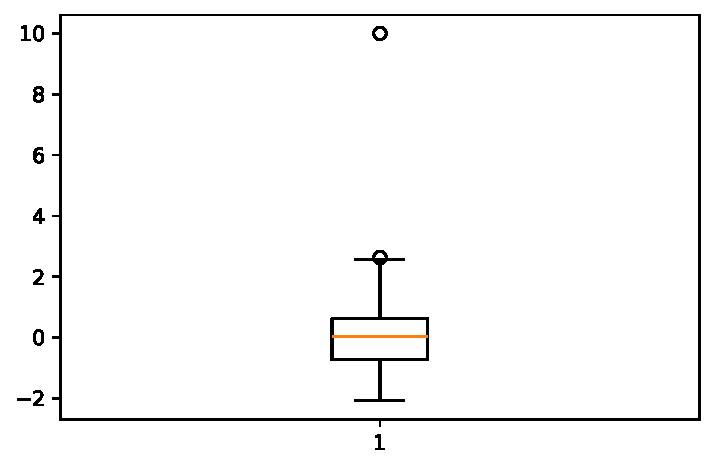
\includegraphics[keepaspectratio]{course/chapters/SEDA/ModelTesting_files/figure-pdf/cell-11-output-1.pdf}}

For more information on outlier detection, refer to the
\href{https://scikit-learn.org/stable/modules/outlier_detection.html}{Scikit-learn
documentation}.

\section*{Example: Model Testing}\label{example-model-testing}
\addcontentsline{toc}{section}{Example: Model Testing}

\markright{Example: Model Testing}

\chapter*{Exercises}\label{exercises-5}
\addcontentsline{toc}{chapter}{Exercises}

\markboth{Exercises}{Exercises}

Download it locally and try to solve the exercises.

\href{https://github.com/stkroe/PythonforChemists/blob/main/course/examples/ModelTesting_Example.ipynb}{Model
Testing Example}

Or open it in \texttt{Google\ Colab}:

\href{https://colab.research.google.com/github/stkroe/PythonforChemists/blob/main/course/examples/ModelTesting_Example.ipynb}{Model
Testing Example}

\chapter{Inferential Statistics}\label{inferential-statistics}

Difficulty level: { }

\chapter*{Data Models}\label{data-models}
\addcontentsline{toc}{chapter}{Data Models}

\markboth{Data Models}{Data Models}

\section*{Linear Regression~}\label{linear-regression}
\addcontentsline{toc}{section}{Linear Regression~}

\markright{Linear Regression~}

Often we want to find a model which can explain the data. It is
important to understand the data and the model to be able to interpret
the results and make predictions.

The simplest model is the linear regression model. It assumes that the
data has a linear relationship with the target variable. For example, if
we have a single feature \(x\) and a target variable \(y\), the linear
regression model can be defined as:

\[
y = \beta_0 + \beta_1 x + \epsilon
\]

where \(y\) is the target variable, \(x\) is the feature, \(\beta_0\)
and \(\beta_1\) are the coefficients, and \(\epsilon\) is the error
term.

For multiple features \(x_1, x_2, \ldots, x_n\), the linear regression
model can be defined as:

\[
y = \beta_0 + \beta_1 x_1 + \beta_2 x_2 + \ldots + \beta_n x_n + \epsilon
\]

where \(y\) is the target variable, \(x_1, x_2, \ldots, x_n\) are the
features, \(\beta_0, \beta_1, \ldots, \beta_n\) are the coefficients,
and \(\epsilon\) is the error term.

In \texttt{python} there exists serveral libraries which can be used to
fit a linear regression model.

\subsection{\texorpdfstring{Using
\texttt{scipy}}{Using scipy}}\label{using-scipy}

A easy way is to use \texttt{scipy} library. The \texttt{scipy} library
has a function called \texttt{linregress} which can be used to fit a
linear regression model. The function returns the slope, intercept,
r-value, p-value, and the standard error of the estimate. And with scipy
version 1.15.2 also the intercept error.

\begin{Shaded}
\begin{Highlighting}[]
\ImportTok{from}\NormalTok{ scipy.stats }\ImportTok{import}\NormalTok{ linregress}
\ImportTok{import}\NormalTok{ numpy }\ImportTok{as}\NormalTok{ np}

\NormalTok{x }\OperatorTok{=}\NormalTok{ [}\DecValTok{1}\NormalTok{, }\DecValTok{2}\NormalTok{, }\DecValTok{3}\NormalTok{, }\DecValTok{4}\NormalTok{, }\DecValTok{5}\NormalTok{]}
\NormalTok{y }\OperatorTok{=}\NormalTok{ x}\OperatorTok{*}\NormalTok{np.random.normal(}\DecValTok{0}\NormalTok{, }\DecValTok{1}\NormalTok{, }\DecValTok{5}\NormalTok{)}\OperatorTok{+}\NormalTok{np.random.normal(}\DecValTok{0}\NormalTok{, }\DecValTok{1}\NormalTok{, }\DecValTok{5}\NormalTok{)}

\NormalTok{results }\OperatorTok{=}\NormalTok{ linregress(x, y)}

\NormalTok{slope }\OperatorTok{=}\NormalTok{ results.slope}
\NormalTok{intercept }\OperatorTok{=}\NormalTok{ results.intercept}
\NormalTok{r\_value }\OperatorTok{=}\NormalTok{ results.rvalue}
\NormalTok{p\_value }\OperatorTok{=}\NormalTok{ results.pvalue}
\NormalTok{std\_err }\OperatorTok{=}\NormalTok{ results.stderr}
\NormalTok{intercept\_err }\OperatorTok{=}\NormalTok{ results.intercept\_stderr}
\BuiltInTok{print}\NormalTok{(}\StringTok{"slope: }\SpecialCharTok{\%f}\StringTok{    intercept: }\SpecialCharTok{\%f}\StringTok{"} \OperatorTok{\%}\NormalTok{ (slope, intercept))}
\BuiltInTok{print}\NormalTok{(}\StringTok{"R{-}squared: }\SpecialCharTok{\%f}\StringTok{"} \OperatorTok{\%}\NormalTok{ r\_value}\OperatorTok{**}\DecValTok{2}\NormalTok{)}
\BuiltInTok{print}\NormalTok{(}\StringTok{"p{-}value: }\SpecialCharTok{\%f}\StringTok{"} \OperatorTok{\%}\NormalTok{ p\_value)}
\BuiltInTok{print}\NormalTok{(}\StringTok{"standard error: }\SpecialCharTok{\%f}\StringTok{"} \OperatorTok{\%}\NormalTok{ std\_err)}
\BuiltInTok{print}\NormalTok{(}\StringTok{"Intercept error: }\SpecialCharTok{\%f}\StringTok{"} \OperatorTok{\%}\NormalTok{intercept\_err)}
\CommentTok{\# Two{-}sided inverse Students t{-}distribution}
\CommentTok{\# p {-} probability, df {-} degrees of freedom}
\ImportTok{from}\NormalTok{ scipy.stats }\ImportTok{import}\NormalTok{ t}
\NormalTok{tinv }\OperatorTok{=} \KeywordTok{lambda}\NormalTok{ p, df: }\BuiltInTok{abs}\NormalTok{(t.ppf(p}\OperatorTok{/}\DecValTok{2}\NormalTok{, df))}
\BuiltInTok{print}\NormalTok{(}\StringTok{"95}\SpecialCharTok{\% c}\StringTok{onfidence interval: "} \OperatorTok{+} \BuiltInTok{str}\NormalTok{(intercept }\OperatorTok{{-}}\NormalTok{ tinv(}\FloatTok{0.05}\NormalTok{, }\BuiltInTok{len}\NormalTok{(x)}\OperatorTok{{-}}\DecValTok{2}\NormalTok{)}\OperatorTok{*}\NormalTok{intercept\_err) }\OperatorTok{+} \StringTok{" to "} \OperatorTok{+} \BuiltInTok{str}\NormalTok{(intercept }\OperatorTok{+}\NormalTok{ tinv(}\FloatTok{0.05}\NormalTok{, }\BuiltInTok{len}\NormalTok{(x)}\OperatorTok{{-}}\DecValTok{2}\NormalTok{)}\OperatorTok{*}\NormalTok{intercept\_err))}
\end{Highlighting}
\end{Shaded}

\begin{verbatim}
slope: 1.561849    intercept: -3.052131
R-squared: 0.745257
p-value: 0.059423
standard error: 0.527202
Intercept error: 1.748531
95% confidence interval: -8.61673825839533 to 2.5124765794392263
\end{verbatim}

\begin{tcolorbox}[enhanced jigsaw, leftrule=.75mm, bottomrule=.15mm, colbacktitle=quarto-callout-important-color!10!white, title=\textcolor{quarto-callout-important-color}{\faExclamation}\hspace{0.5em}{Important}, breakable, arc=.35mm, toptitle=1mm, opacityback=0, titlerule=0mm, coltitle=black, colback=white, opacitybacktitle=0.6, colframe=quarto-callout-important-color-frame, left=2mm, rightrule=.15mm, toprule=.15mm, bottomtitle=1mm]

For older version \texttt{scipy}only returned 5 values with fields
slope, intercept, rvalue, pvalue and stderr. For compatiblity reasons
the return values are 5 elements tuple.

\begin{Shaded}
\begin{Highlighting}[]
\ImportTok{from}\NormalTok{ scipy.stats }\ImportTok{import}\NormalTok{ linregress}
\NormalTok{slope, intercept, r, p, se }\OperatorTok{=}\NormalTok{ linregress(x, y)}
\BuiltInTok{print}\NormalTok{(}\StringTok{"slope: "}\NormalTok{, slope)}
\BuiltInTok{print}\NormalTok{(}\StringTok{"intercept: "}\NormalTok{, intercept)}
\BuiltInTok{print}\NormalTok{(}\StringTok{"r{-}value: "}\NormalTok{, r)}
\BuiltInTok{print}\NormalTok{(}\StringTok{"p{-}value: "}\NormalTok{, p)}
\BuiltInTok{print}\NormalTok{(}\StringTok{"standard error: "}\NormalTok{, se)}
\end{Highlighting}
\end{Shaded}

\begin{verbatim}
slope:  1.561849163253334
intercept:  -3.052130839478052
r-value:  0.8632824131244606
p-value:  0.059423389317344436
standard error:  0.527202065322916
\end{verbatim}

And if you want to get the intercept error you can use the following
return value as a object:

\begin{Shaded}
\begin{Highlighting}[]
\ImportTok{from}\NormalTok{ scipy.stats }\ImportTok{import}\NormalTok{ linregress}
\NormalTok{results }\OperatorTok{=}\NormalTok{ linregress(x, y)}
\BuiltInTok{print}\NormalTok{(}\StringTok{"slope: "}\NormalTok{, results.slope)}
\BuiltInTok{print}\NormalTok{(}\StringTok{"intercept: "}\NormalTok{, results.intercept)}
\BuiltInTok{print}\NormalTok{(}\StringTok{"r{-}value: "}\NormalTok{, results.rvalue)}
\BuiltInTok{print}\NormalTok{(}\StringTok{"p{-}value: "}\NormalTok{, results.pvalue)}
\BuiltInTok{print}\NormalTok{(}\StringTok{"standard error: "}\NormalTok{, results.stderr)}
\BuiltInTok{print}\NormalTok{(}\StringTok{"intercept error: "}\NormalTok{, results.intercept\_stderr)}
\end{Highlighting}
\end{Shaded}

\begin{verbatim}
slope:  1.561849163253334
intercept:  -3.052130839478052
r-value:  0.8632824131244606
p-value:  0.059423389317344436
standard error:  0.527202065322916
intercept error:  1.74853143937655
\end{verbatim}

\end{tcolorbox}

\subsection{\texorpdfstring{Using
\texttt{statsmodels}}{Using statsmodels}}\label{using-statsmodels}

Another library is \texttt{statsmodels}. The \texttt{statsmodels}
library provides more detailed information about the model, such as the
coefficients, standard errors, t-values, p-values, and confidence
intervals.

\begin{Shaded}
\begin{Highlighting}[]
\ImportTok{import}\NormalTok{ statsmodels.api }\ImportTok{as}\NormalTok{ sm}
\ImportTok{import}\NormalTok{ numpy }\ImportTok{as}\NormalTok{ np}

\NormalTok{X }\OperatorTok{=}\NormalTok{ np.array([}\DecValTok{1}\NormalTok{, }\DecValTok{2}\NormalTok{, }\DecValTok{3}\NormalTok{, }\DecValTok{4}\NormalTok{, }\DecValTok{5}\NormalTok{])}
\NormalTok{y }\OperatorTok{=}\NormalTok{ X}\OperatorTok{*}\NormalTok{np.random.normal(}\DecValTok{0}\NormalTok{, }\DecValTok{1}\NormalTok{, }\DecValTok{5}\NormalTok{)}\OperatorTok{+}\NormalTok{np.random.normal(}\DecValTok{0}\NormalTok{, }\DecValTok{1}\NormalTok{, }\DecValTok{5}\NormalTok{)}

\NormalTok{X\_with\_const }\OperatorTok{=}\NormalTok{ sm.add\_constant(X)  }\CommentTok{\# Add intercept term}
\NormalTok{model }\OperatorTok{=}\NormalTok{ sm.OLS(y, X\_with\_const).fit()}
\BuiltInTok{print}\NormalTok{(model.summary())}
\end{Highlighting}
\end{Shaded}

\begin{verbatim}
                            OLS Regression Results                            
==============================================================================
Dep. Variable:                      y   R-squared:                       0.031
Model:                            OLS   Adj. R-squared:                 -0.292
Method:                 Least Squares   F-statistic:                   0.09623
Date:                Fri, 11 Apr 2025   Prob (F-statistic):              0.777
Time:                        10:41:31   Log-Likelihood:                -13.663
No. Observations:                   5   AIC:                             31.33
Df Residuals:                       3   BIC:                             30.54
Df Model:                           1                                         
Covariance Type:            nonrobust                                         
==============================================================================
                 coef    std err          t      P>|t|      [0.025      0.975]
------------------------------------------------------------------------------
const          2.4040      5.036      0.477      0.666     -13.624      18.431
x1            -0.4711      1.518     -0.310      0.777      -5.304       4.361
==============================================================================
Omnibus:                          nan   Durbin-Watson:                   1.941
Prob(Omnibus):                    nan   Jarque-Bera (JB):                0.408
Skew:                          -0.100   Prob(JB):                        0.815
Kurtosis:                       1.615   Cond. No.                         8.37
==============================================================================

Notes:
[1] Standard Errors assume that the covariance matrix of the errors is correctly specified.
\end{verbatim}

\subsection*{\texorpdfstring{Using
\texttt{scikit-learn}}{Using scikit-learn}}\label{using-scikit-learn}
\addcontentsline{toc}{subsection}{Using \texttt{scikit-learn}}

One of the most popular libraries is \texttt{scikit-learn}. The
following code shows how to fit a linear regression model using
\texttt{scikit-learn}:

\begin{Shaded}
\begin{Highlighting}[]
\ImportTok{from}\NormalTok{ sklearn.linear\_model }\ImportTok{import}\NormalTok{ LinearRegression}
\ImportTok{import}\NormalTok{ numpy }\ImportTok{as}\NormalTok{ np}
\ImportTok{import}\NormalTok{ matplotlib.pyplot }\ImportTok{as}\NormalTok{ plt}

\CommentTok{\# Sample data}
\NormalTok{X }\OperatorTok{=}\NormalTok{ np.linspace(}\DecValTok{1}\NormalTok{, }\DecValTok{5}\NormalTok{, }\DecValTok{100}\NormalTok{).reshape(}\OperatorTok{{-}}\DecValTok{1}\NormalTok{, }\DecValTok{1}\NormalTok{)}
\NormalTok{y }\OperatorTok{=} \DecValTok{2} \OperatorTok{*}\NormalTok{ X }\OperatorTok{+} \DecValTok{1} \OperatorTok{+}\NormalTok{ np.random.normal(}\DecValTok{0}\NormalTok{, }\DecValTok{1}\NormalTok{, }\DecValTok{100}\NormalTok{).reshape(}\OperatorTok{{-}}\DecValTok{1}\NormalTok{, }\DecValTok{1}\NormalTok{)}

\CommentTok{\# Model fitting}
\NormalTok{model }\OperatorTok{=}\NormalTok{ LinearRegression()}
\NormalTok{model.fit(X, y)}
\BuiltInTok{print}\NormalTok{(}\StringTok{"Parameters:"}\NormalTok{, model.get\_params())}
\BuiltInTok{print}\NormalTok{(}\StringTok{"R{-}squared:"}\NormalTok{, model.score(X, y))}

\CommentTok{\# Predictions}
\NormalTok{y\_pred }\OperatorTok{=}\NormalTok{ model.predict(X)}

\CommentTok{\# Plot}
\NormalTok{plt.scatter(X, y, color}\OperatorTok{=}\StringTok{\textquotesingle{}blue\textquotesingle{}}\NormalTok{, label}\OperatorTok{=}\StringTok{\textquotesingle{}Data\textquotesingle{}}\NormalTok{)}
\NormalTok{plt.plot(X, y\_pred, color}\OperatorTok{=}\StringTok{\textquotesingle{}red\textquotesingle{}}\NormalTok{, label}\OperatorTok{=}\StringTok{\textquotesingle{}Linear Fit\textquotesingle{}}\NormalTok{)}
\NormalTok{plt.legend()}
\NormalTok{plt.show()}
\end{Highlighting}
\end{Shaded}

\begin{verbatim}
Parameters: {'copy_X': True, 'fit_intercept': True, 'n_jobs': None, 'positive': False}
R-squared: 0.8698274418684563
\end{verbatim}

\pandocbounded{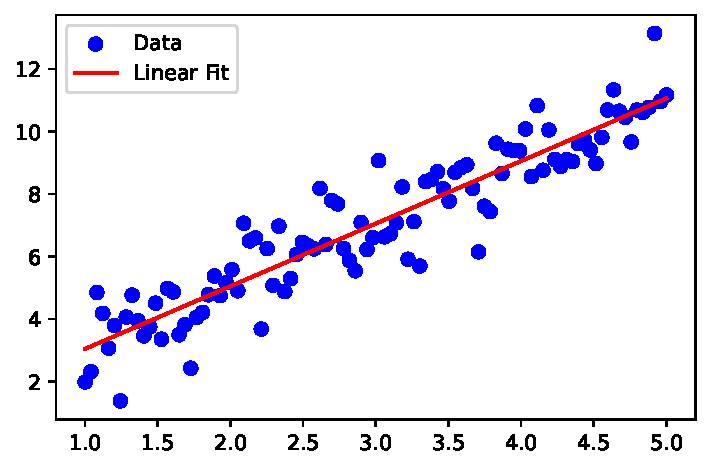
\includegraphics[keepaspectratio]{course/chapters/SEDA/DataModels_files/figure-pdf/cell-6-output-2.pdf}}

\begin{center}\rule{0.5\linewidth}{0.5pt}\end{center}

\section{Non-Linear Fits}\label{non-linear-fits}

Linear regression may not always be sufficient, especially for complex
relationships. Non-linear models provide more flexibility.

\subsection{Polynomial Regression}\label{polynomial-regression}

Polynomial regression is a type of linear regression where the
relationship between the independent variable \(x\) and the dependent
variable \(y\) is modeled as an \(n\)-th degree polynomial.

\begin{Shaded}
\begin{Highlighting}[]
\ImportTok{import}\NormalTok{ numpy }\ImportTok{as}\NormalTok{ np}
\ImportTok{import}\NormalTok{ matplotlib.pyplot }\ImportTok{as}\NormalTok{ plt}


\CommentTok{\# Sample data}
\NormalTok{X }\OperatorTok{=}\NormalTok{ np.linspace(}\DecValTok{1}\NormalTok{, }\DecValTok{5}\NormalTok{, }\DecValTok{100}\NormalTok{)}
\NormalTok{y }\OperatorTok{=}\NormalTok{ X}\OperatorTok{**}\DecValTok{2} \OperatorTok{+}\NormalTok{ np.random.normal(}\DecValTok{0}\NormalTok{, }\DecValTok{1}\NormalTok{, }\DecValTok{100}\NormalTok{)}

\NormalTok{model }\OperatorTok{=}\NormalTok{ np.polyfit(X, y, }\DecValTok{2}\NormalTok{)}

\BuiltInTok{print}\NormalTok{(}\StringTok{"Coefficients:"}\NormalTok{, model)}

\CommentTok{\# Create a polynomial function}

\NormalTok{model }\OperatorTok{=}\NormalTok{ np.poly1d(model)}

\NormalTok{X\_range }\OperatorTok{=}\NormalTok{ np.linspace(}\DecValTok{1}\NormalTok{, }\DecValTok{5}\NormalTok{, }\DecValTok{100}\NormalTok{)}
\NormalTok{y\_fit }\OperatorTok{=}\NormalTok{ model(X\_range)}

\BuiltInTok{print}\NormalTok{(model)}

\NormalTok{plt.scatter(X, y, color}\OperatorTok{=}\StringTok{\textquotesingle{}blue\textquotesingle{}}\NormalTok{, label}\OperatorTok{=}\StringTok{\textquotesingle{}Data\textquotesingle{}}\NormalTok{)}
\NormalTok{plt.plot(X\_range, y\_fit, color}\OperatorTok{=}\StringTok{\textquotesingle{}purple\textquotesingle{}}\NormalTok{, label}\OperatorTok{=}\StringTok{\textquotesingle{}Polynomial Fit\textquotesingle{}}\NormalTok{)}
\NormalTok{plt.legend()}
\end{Highlighting}
\end{Shaded}

\begin{verbatim}
Coefficients: [ 0.85020179  0.84927237 -1.05865633]
        2
0.8502 x + 0.8493 x - 1.059
\end{verbatim}

\pandocbounded{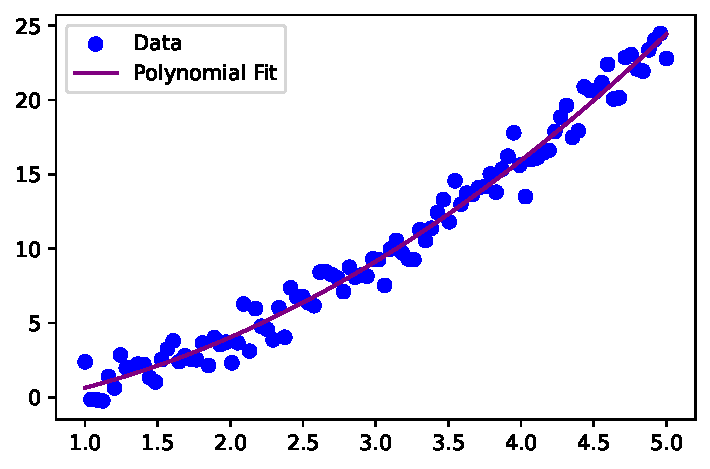
\includegraphics[keepaspectratio]{course/chapters/SEDA/DataModels_files/figure-pdf/cell-7-output-2.pdf}}

\subsection{\texorpdfstring{Curve Fitting with
\texttt{scipy}}{Curve Fitting with scipy}}\label{curve-fitting-with-scipy}

\texttt{scipy} provides the \texttt{curve\_fit} function to fit a
non-linear model to the data. The function requires the model function
and the data as input.

\begin{Shaded}
\begin{Highlighting}[]
\ImportTok{from}\NormalTok{ scipy.optimize }\ImportTok{import}\NormalTok{ curve\_fit}

\KeywordTok{def}\NormalTok{ nonlinear\_func(x, a, b, c):}
    \ControlFlowTok{return}\NormalTok{ a }\OperatorTok{*}\NormalTok{ np.sin(b }\OperatorTok{*}\NormalTok{ x) }\OperatorTok{+}\NormalTok{ c}

\NormalTok{popt,pov  }\OperatorTok{=}\NormalTok{ curve\_fit(nonlinear\_func, X.flatten(), y)}
\NormalTok{perr }\OperatorTok{=}\NormalTok{ np.sqrt(np.diag(pov))}

\BuiltInTok{print}\NormalTok{(}\StringTok{"Fitted parameters:"}\NormalTok{, popt)}
\BuiltInTok{print}\NormalTok{(}\StringTok{"Parameter errors:"}\NormalTok{, perr)}

\NormalTok{X\_range }\OperatorTok{=}\NormalTok{ np.linspace(}\DecValTok{1}\NormalTok{, }\DecValTok{5}\NormalTok{, }\DecValTok{100}\NormalTok{)}
\NormalTok{y\_fit }\OperatorTok{=}\NormalTok{ nonlinear\_func(X\_range, }\OperatorTok{*}\NormalTok{popt)}

\NormalTok{plt.scatter(X, y, color}\OperatorTok{=}\StringTok{\textquotesingle{}blue\textquotesingle{}}\NormalTok{, label}\OperatorTok{=}\StringTok{\textquotesingle{}Data\textquotesingle{}}\NormalTok{)}
\NormalTok{plt.plot(X\_range, y\_fit, color}\OperatorTok{=}\StringTok{\textquotesingle{}purple\textquotesingle{}}\NormalTok{, label}\OperatorTok{=}\StringTok{\textquotesingle{}Non{-}Linear Fit\textquotesingle{}}\NormalTok{)}
\NormalTok{plt.legend()}
\NormalTok{plt.show()}
\end{Highlighting}
\end{Shaded}

\begin{verbatim}
Fitted parameters: [-9.54970511  0.92619133 12.0288274 ]
Parameter errors: [0.27053402 0.01453711 0.31589986]
\end{verbatim}

\pandocbounded{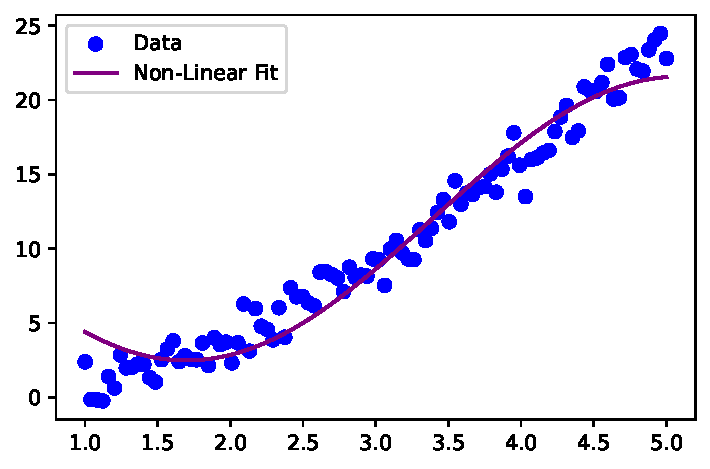
\includegraphics[keepaspectratio]{course/chapters/SEDA/DataModels_files/figure-pdf/cell-8-output-2.pdf}}

\chapter{Advanced Statistical
Analysis}\label{advanced-statistical-analysis}

Difficulty level: { }

Often data has multi dimensions and it is not easy to analyze it.
Multivariate analysis is a set of statistical techniques used to analyze
data with multiple variables. It helps in understanding the
relationships between variables and identifying patterns in complex
data.

What can be done to analyze multi-dimensional data?

\begin{itemize}
\tightlist
\item
  \textbf{Dimensionality Reduction:} Simplifies complex datasets by
  reducing the number of variables.
\item
  \textbf{Pattern Recognition:} Identifies underlying patterns and
  trends in data.
\item
  \textbf{Feature Selection:} Selects relevant variables for modeling
  and prediction.
\end{itemize}

\section*{Dimensionality Reduction
Techniques}\label{dimensionality-reduction-techniques}
\addcontentsline{toc}{section}{Dimensionality Reduction Techniques}

\markright{Dimensionality Reduction Techniques}

\textbf{Principal Component Analysis (PCA):} reduces the dimensionality
of data by transforming variables into uncorrelated components. It
retains most of the variance in the data while reducing noise and
redundancy. The PCA decomposition is based on the eigenvalues and
eigenvectors of the covariance matrix of the data to identify the
principal components with the highest variance.

\begin{Shaded}
\begin{Highlighting}[]
\ImportTok{import}\NormalTok{ numpy }\ImportTok{as}\NormalTok{ np}
\ImportTok{import}\NormalTok{ matplotlib.pyplot }\ImportTok{as}\NormalTok{ plt}
\ImportTok{from}\NormalTok{ sklearn.decomposition }\ImportTok{import}\NormalTok{ PCA}

\CommentTok{\# Create a simple 2D dataset}
\NormalTok{X }\OperatorTok{=}\NormalTok{ np.array([}
\NormalTok{    [}\FloatTok{2.5}\NormalTok{, }\FloatTok{2.4}\NormalTok{],}
\NormalTok{    [}\FloatTok{0.5}\NormalTok{, }\FloatTok{0.7}\NormalTok{],}
\NormalTok{    [}\FloatTok{2.2}\NormalTok{, }\FloatTok{2.9}\NormalTok{],}
\NormalTok{    [}\FloatTok{1.9}\NormalTok{, }\FloatTok{2.2}\NormalTok{],}
\NormalTok{    [}\FloatTok{3.1}\NormalTok{, }\FloatTok{3.0}\NormalTok{],}
\NormalTok{    [}\FloatTok{2.3}\NormalTok{, }\FloatTok{2.7}\NormalTok{],}
\NormalTok{    [}\DecValTok{2}\NormalTok{, }\FloatTok{1.6}\NormalTok{],}
\NormalTok{    [}\DecValTok{1}\NormalTok{, }\FloatTok{1.1}\NormalTok{],}
\NormalTok{    [}\FloatTok{1.5}\NormalTok{, }\FloatTok{1.6}\NormalTok{],}
\NormalTok{    [}\FloatTok{1.1}\NormalTok{, }\FloatTok{0.9}\NormalTok{]}
\NormalTok{])}

\CommentTok{\# Plot original data}
\NormalTok{plt.figure(figsize}\OperatorTok{=}\NormalTok{(}\DecValTok{6}\NormalTok{, }\DecValTok{6}\NormalTok{))}
\NormalTok{plt.scatter(X[:, }\DecValTok{0}\NormalTok{], X[:, }\DecValTok{1}\NormalTok{], color}\OperatorTok{=}\StringTok{\textquotesingle{}blue\textquotesingle{}}\NormalTok{)}
\NormalTok{plt.title(}\StringTok{"Original 2D Data"}\NormalTok{)}
\NormalTok{plt.xlabel(}\StringTok{"Feature 1"}\NormalTok{)}
\NormalTok{plt.ylabel(}\StringTok{"Feature 2"}\NormalTok{)}
\NormalTok{plt.axis(}\StringTok{"equal"}\NormalTok{)}
\NormalTok{plt.grid(}\VariableTok{True}\NormalTok{)}
\NormalTok{plt.show()}

\CommentTok{\# Apply PCA to reduce to 1D}
\NormalTok{pca }\OperatorTok{=}\NormalTok{ PCA(n\_components}\OperatorTok{=}\DecValTok{1}\NormalTok{)}
\NormalTok{X\_pca }\OperatorTok{=}\NormalTok{ pca.fit\_transform(X)}
\NormalTok{X\_projected }\OperatorTok{=}\NormalTok{ pca.inverse\_transform(X\_pca)}

\CommentTok{\# Plot the projected data}
\NormalTok{plt.figure(figsize}\OperatorTok{=}\NormalTok{(}\DecValTok{6}\NormalTok{, }\DecValTok{6}\NormalTok{))}
\NormalTok{plt.scatter(X[:, }\DecValTok{0}\NormalTok{], X[:, }\DecValTok{1}\NormalTok{], label}\OperatorTok{=}\StringTok{\textquotesingle{}Original\textquotesingle{}}\NormalTok{, alpha}\OperatorTok{=}\FloatTok{0.6}\NormalTok{)}
\NormalTok{plt.scatter(X\_projected[:, }\DecValTok{0}\NormalTok{], X\_projected[:, }\DecValTok{1}\NormalTok{], label}\OperatorTok{=}\StringTok{\textquotesingle{}Projected (1D)\textquotesingle{}}\NormalTok{, alpha}\OperatorTok{=}\FloatTok{0.6}\NormalTok{)}
\ControlFlowTok{for}\NormalTok{ orig, proj }\KeywordTok{in} \BuiltInTok{zip}\NormalTok{(X, X\_projected):}
\NormalTok{    plt.plot([orig[}\DecValTok{0}\NormalTok{], proj[}\DecValTok{0}\NormalTok{]], [orig[}\DecValTok{1}\NormalTok{], proj[}\DecValTok{1}\NormalTok{]], }\StringTok{\textquotesingle{}r{-}{-}\textquotesingle{}}\NormalTok{, linewidth}\OperatorTok{=}\FloatTok{0.5}\NormalTok{)}
\NormalTok{plt.title(}\StringTok{"PCA Projection to 1D"}\NormalTok{)}
\NormalTok{plt.xlabel(}\StringTok{"Feature 1"}\NormalTok{)}
\NormalTok{plt.ylabel(}\StringTok{"Feature 2"}\NormalTok{)}
\NormalTok{plt.legend()}
\NormalTok{plt.axis(}\StringTok{"equal"}\NormalTok{)}
\NormalTok{plt.grid(}\VariableTok{True}\NormalTok{)}
\NormalTok{plt.show()}
\end{Highlighting}
\end{Shaded}

\pandocbounded{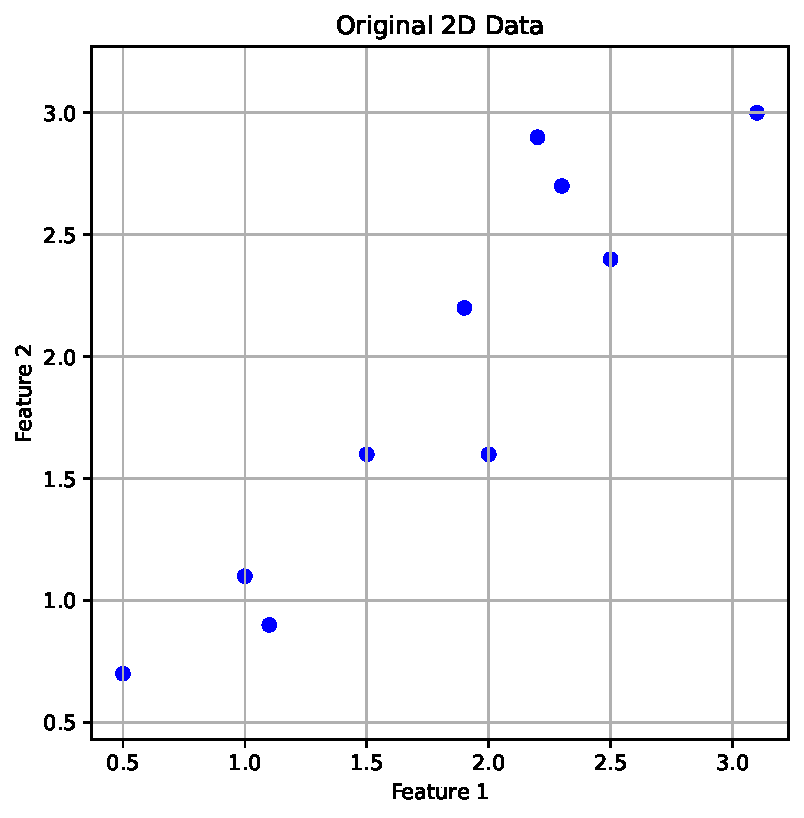
\includegraphics[keepaspectratio]{course/chapters/SEDA/AdvancedAnalysis_files/figure-pdf/cell-2-output-1.pdf}}

\pandocbounded{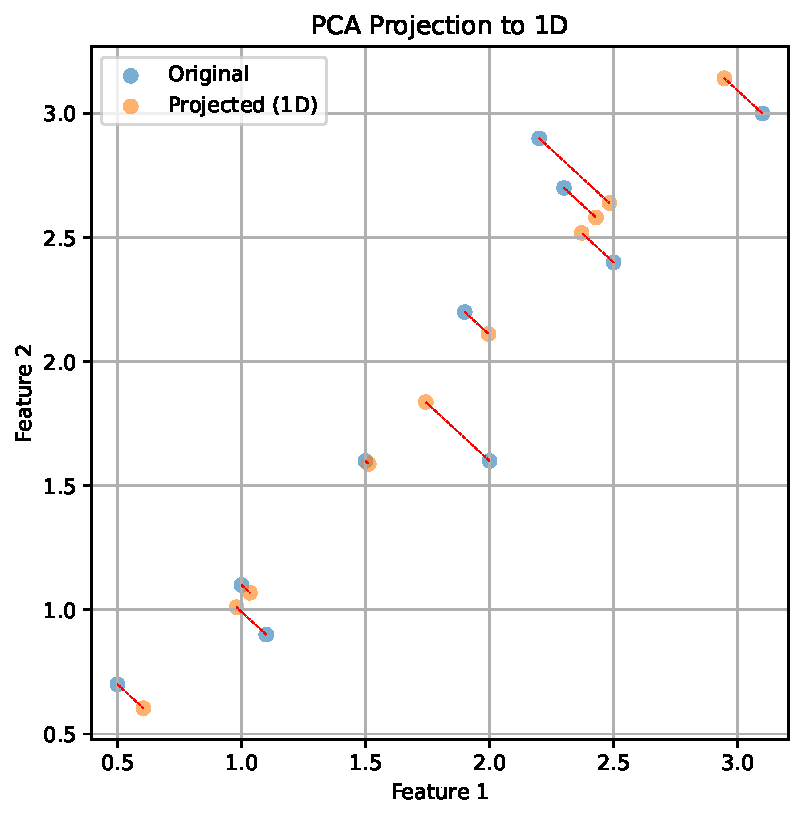
\includegraphics[keepaspectratio]{course/chapters/SEDA/AdvancedAnalysis_files/figure-pdf/cell-2-output-2.pdf}}

Sometimes the data needs to be scaled before applying PCA. The
\texttt{StandardScaler} from \texttt{sklearn} can be used to scale the
data.

\begin{Shaded}
\begin{Highlighting}[]
\ImportTok{import}\NormalTok{ numpy }\ImportTok{as}\NormalTok{ np}
\ImportTok{import}\NormalTok{ matplotlib.pyplot }\ImportTok{as}\NormalTok{ plt}
\ImportTok{from}\NormalTok{ sklearn.preprocessing }\ImportTok{import}\NormalTok{ StandardScaler}
\ImportTok{from}\NormalTok{ sklearn.decomposition }\ImportTok{import}\NormalTok{ PCA}

\CommentTok{\# Generate synthetic data}
\NormalTok{rng }\OperatorTok{=}\NormalTok{ np.random.RandomState(}\DecValTok{0}\NormalTok{)}
\NormalTok{n\_samples }\OperatorTok{=} \DecValTok{100}
\NormalTok{cov }\OperatorTok{=}\NormalTok{ [[}\DecValTok{6}\NormalTok{, }\DecValTok{1}\NormalTok{], [}\DecValTok{8}\NormalTok{, }\DecValTok{4}\NormalTok{]]}
\NormalTok{X }\OperatorTok{=}\NormalTok{ rng.multivariate\_normal(mean}\OperatorTok{=}\NormalTok{[}\DecValTok{0}\NormalTok{, }\DecValTok{0}\NormalTok{], cov}\OperatorTok{=}\NormalTok{cov, size}\OperatorTok{=}\NormalTok{n\_samples)}

\CommentTok{\# Standardizing Data}
\NormalTok{scaler }\OperatorTok{=}\NormalTok{ StandardScaler()}
\NormalTok{X\_scaled }\OperatorTok{=}\NormalTok{ scaler.fit\_transform(X)}

\CommentTok{\# Applying PCA}
\NormalTok{pca }\OperatorTok{=}\NormalTok{ PCA(n\_components}\OperatorTok{=}\DecValTok{2}\NormalTok{)}
\NormalTok{X\_pca }\OperatorTok{=}\NormalTok{ pca.fit\_transform(X\_scaled)}

\BuiltInTok{print}\NormalTok{(}\StringTok{"Explained Variance Ratio:"}\NormalTok{, pca.explained\_variance\_ratio\_)}

\CommentTok{\# Plot PCA results}
\NormalTok{plt.scatter(X\_pca[:, }\DecValTok{0}\NormalTok{], X\_pca[:, }\DecValTok{1}\NormalTok{])}
\NormalTok{plt.xlabel(}\StringTok{\textquotesingle{}PC1\textquotesingle{}}\NormalTok{)}
\NormalTok{plt.ylabel(}\StringTok{\textquotesingle{}PC2\textquotesingle{}}\NormalTok{)}
\NormalTok{plt.title(}\StringTok{\textquotesingle{}PCA Analysis\textquotesingle{}}\NormalTok{)}
\NormalTok{plt.show()}
\end{Highlighting}
\end{Shaded}

\begin{verbatim}
Explained Variance Ratio: [0.81292552 0.18707448]
\end{verbatim}

\pandocbounded{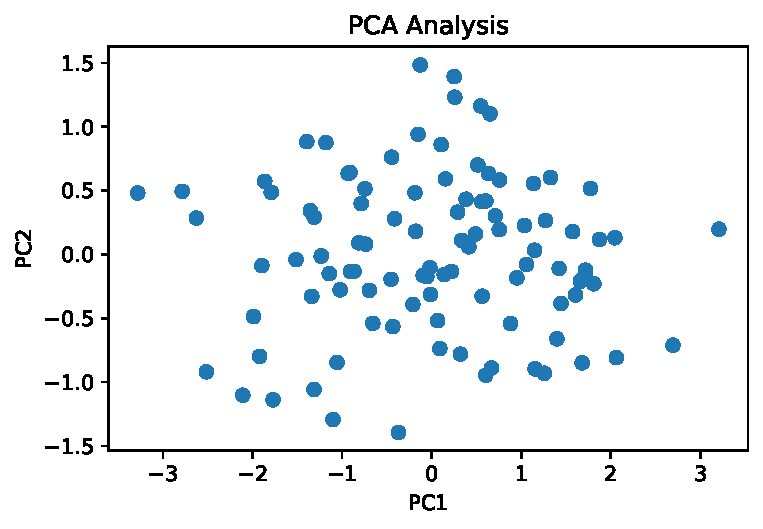
\includegraphics[keepaspectratio]{course/chapters/SEDA/AdvancedAnalysis_files/figure-pdf/cell-3-output-2.pdf}}

\textbf{PCR (Principal Component Regression):} Combines PCA and
regression analysis. It first applies PCA to reduce dimensionality and
then performs regression on the principal components. (see for more
information
\url{https://en.wikipedia.org/wiki/Principal_component_regression} and
\url{https://scikit-learn.org/stable/auto_examples/cross_decomposition/plot_pcr_vs_pls.html}

\begin{Shaded}
\begin{Highlighting}[]
\ImportTok{import}\NormalTok{ numpy }\ImportTok{as}\NormalTok{ np}
\ImportTok{import}\NormalTok{ matplotlib.pyplot }\ImportTok{as}\NormalTok{ plt}

\ImportTok{from}\NormalTok{ sklearn.decomposition }\ImportTok{import}\NormalTok{ PCA}
\ImportTok{from}\NormalTok{ sklearn.linear\_model }\ImportTok{import}\NormalTok{ LinearRegression}
\ImportTok{from}\NormalTok{ sklearn.pipeline }\ImportTok{import}\NormalTok{ make\_pipeline}
\ImportTok{from}\NormalTok{ sklearn.preprocessing }\ImportTok{import}\NormalTok{ StandardScaler}
\ImportTok{from}\NormalTok{ sklearn.datasets }\ImportTok{import}\NormalTok{ make\_regression}
\ImportTok{from}\NormalTok{ sklearn.model\_selection }\ImportTok{import}\NormalTok{ train\_test\_split}
\CommentTok{\# Generate synthetic data}
\NormalTok{rng }\OperatorTok{=}\NormalTok{ np.random.RandomState(}\DecValTok{0}\NormalTok{)}
\NormalTok{n\_samples }\OperatorTok{=} \DecValTok{100}
\NormalTok{cov }\OperatorTok{=}\NormalTok{ [[}\DecValTok{6}\NormalTok{, }\DecValTok{1}\NormalTok{], [}\DecValTok{8}\NormalTok{, }\DecValTok{4}\NormalTok{]]}
\NormalTok{X }\OperatorTok{=}\NormalTok{ rng.multivariate\_normal(mean}\OperatorTok{=}\NormalTok{[}\DecValTok{3}\NormalTok{, }\DecValTok{5}\NormalTok{], cov}\OperatorTok{=}\NormalTok{cov, size}\OperatorTok{=}\NormalTok{n\_samples)}

\CommentTok{\# generate PCA components}
\NormalTok{pca }\OperatorTok{=}\NormalTok{ PCA(n\_components}\OperatorTok{=}\DecValTok{2}\NormalTok{).fit(X)}
\end{Highlighting}
\end{Shaded}

\textbf{Independent Component Analysis (ICA):} Separates a multivariate
signal into additive subcomponents.

\begin{Shaded}
\begin{Highlighting}[]
\ImportTok{import}\NormalTok{ numpy }\ImportTok{as}\NormalTok{ np}
\ImportTok{import}\NormalTok{ matplotlib.pyplot }\ImportTok{as}\NormalTok{ plt}
\ImportTok{from}\NormalTok{ sklearn.decomposition }\ImportTok{import}\NormalTok{ FastICA}

\CommentTok{\# Sample dataset}
\NormalTok{X }\OperatorTok{=}\NormalTok{ np.random.rand(}\DecValTok{10}\NormalTok{, }\DecValTok{3}\NormalTok{)}
\NormalTok{ica }\OperatorTok{=}\NormalTok{ FastICA(n\_components}\OperatorTok{=}\DecValTok{2}\NormalTok{)}
\NormalTok{X\_ica }\OperatorTok{=}\NormalTok{ ica.fit\_transform(X)}

\CommentTok{\# Plot ICA results}
\NormalTok{plt.scatter(X\_ica[:, }\DecValTok{0}\NormalTok{], X\_ica[:, }\DecValTok{1}\NormalTok{])}
\NormalTok{plt.xlabel(}\StringTok{\textquotesingle{}ICA1\textquotesingle{}}\NormalTok{)}
\NormalTok{plt.ylabel(}\StringTok{\textquotesingle{}ICA2\textquotesingle{}}\NormalTok{)}
\NormalTok{plt.title(}\StringTok{\textquotesingle{}Independent Component Analysis\textquotesingle{}}\NormalTok{)}
\NormalTok{plt.show()}
\end{Highlighting}
\end{Shaded}

\pandocbounded{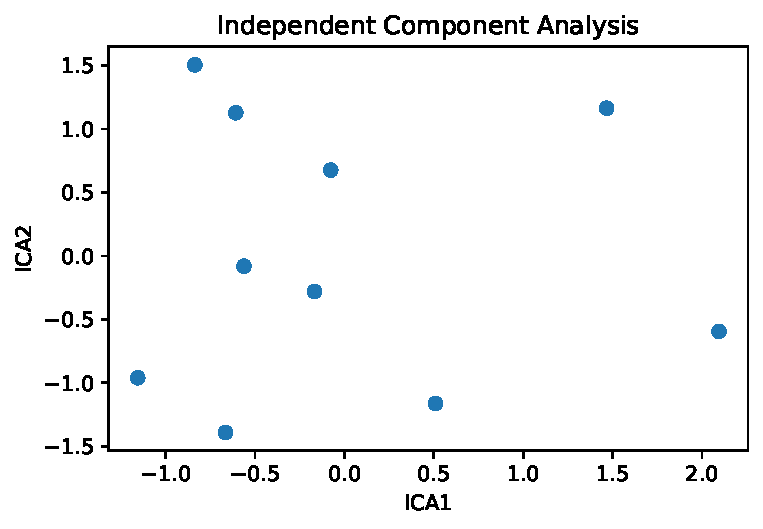
\includegraphics[keepaspectratio]{course/chapters/SEDA/AdvancedAnalysis_files/figure-pdf/cell-5-output-1.pdf}}

\textbf{t-Distributed Stochastic Neighbor Embedding (t-SNE):} Visualizes
high-dimensional data in lower dimensions.

\begin{Shaded}
\begin{Highlighting}[]
\ImportTok{import}\NormalTok{ numpy }\ImportTok{as}\NormalTok{ np}
\ImportTok{import}\NormalTok{ matplotlib.pyplot }\ImportTok{as}\NormalTok{ plt}
\ImportTok{from}\NormalTok{ sklearn.manifold }\ImportTok{import}\NormalTok{ TSNE}

\CommentTok{\# Sample dataset}
\NormalTok{X }\OperatorTok{=}\NormalTok{ np.random.rand(}\DecValTok{10}\NormalTok{, }\DecValTok{3}\NormalTok{)}
\NormalTok{tsne }\OperatorTok{=}\NormalTok{ TSNE(n\_components}\OperatorTok{=}\DecValTok{2}\NormalTok{,perplexity}\OperatorTok{=}\DecValTok{3}\NormalTok{,learning\_rate}\OperatorTok{=}\StringTok{\textquotesingle{}auto\textquotesingle{}}\NormalTok{)}
\NormalTok{X\_tsne }\OperatorTok{=}\NormalTok{ tsne.fit\_transform(X)}

\CommentTok{\# Plot t{-}SNE results}
\NormalTok{plt.scatter(X\_tsne[:, }\DecValTok{0}\NormalTok{], X\_tsne[:, }\DecValTok{1}\NormalTok{])}
\NormalTok{plt.xlabel(}\StringTok{\textquotesingle{}t{-}SNE1\textquotesingle{}}\NormalTok{)}
\NormalTok{plt.ylabel(}\StringTok{\textquotesingle{}t{-}SNE2\textquotesingle{}}\NormalTok{)}
\NormalTok{plt.title(}\StringTok{\textquotesingle{}t{-}SNE Analysis\textquotesingle{}}\NormalTok{)}
\NormalTok{plt.show()}
\end{Highlighting}
\end{Shaded}

\pandocbounded{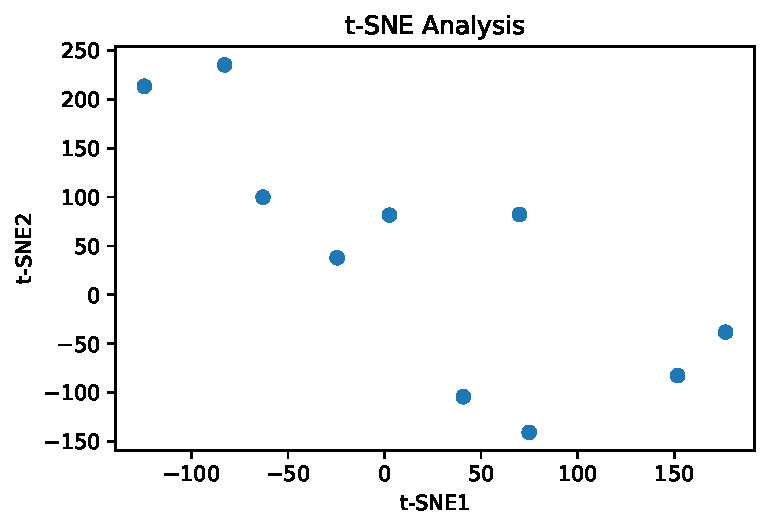
\includegraphics[keepaspectratio]{course/chapters/SEDA/AdvancedAnalysis_files/figure-pdf/cell-6-output-1.pdf}}

\textbf{UMAP (Uniform Manifold Approximation and Projection):} Reduces
the dimensionality of data while preserving local and global structure.

\begin{Shaded}
\begin{Highlighting}[]
\ImportTok{import}\NormalTok{ numpy }\ImportTok{as}\NormalTok{ np}
\ImportTok{import}\NormalTok{ matplotlib.pyplot }\ImportTok{as}\NormalTok{ plt}
\ImportTok{import}\NormalTok{ umap}

\CommentTok{\# Sample dataset}
\NormalTok{X }\OperatorTok{=}\NormalTok{ np.random.rand(}\DecValTok{10}\NormalTok{, }\DecValTok{3}\NormalTok{)}
\NormalTok{umap\_model }\OperatorTok{=}\NormalTok{ umap.UMAP(n\_components}\OperatorTok{=}\DecValTok{2}\NormalTok{)}
\NormalTok{X\_umap }\OperatorTok{=}\NormalTok{ umap\_model.fit\_transform(X)}

\CommentTok{\# Plot UMAP results}
\NormalTok{plt.scatter(X\_umap[:, }\DecValTok{0}\NormalTok{], X\_umap[:, }\DecValTok{1}\NormalTok{])}
\NormalTok{plt.xlabel(}\StringTok{\textquotesingle{}UMAP1\textquotesingle{}}\NormalTok{)}
\NormalTok{plt.ylabel(}\StringTok{\textquotesingle{}UMAP2\textquotesingle{}}\NormalTok{)}
\NormalTok{plt.title(}\StringTok{\textquotesingle{}UMAP Analysis\textquotesingle{}}\NormalTok{)}
\NormalTok{plt.show()}
\end{Highlighting}
\end{Shaded}

\pandocbounded{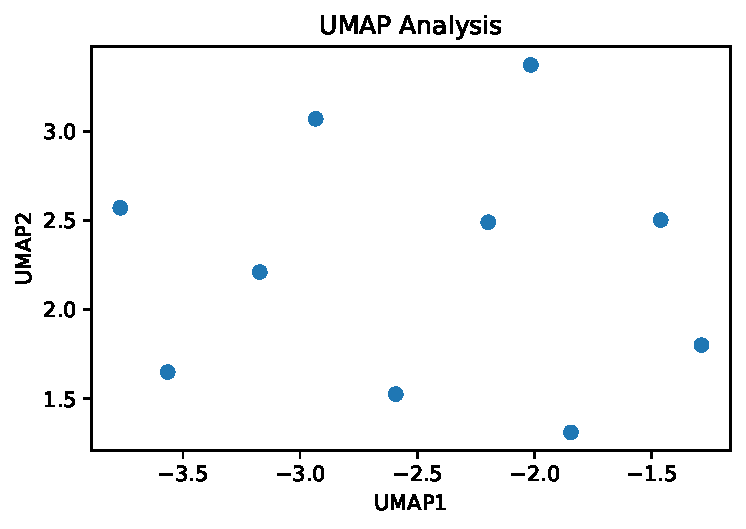
\includegraphics[keepaspectratio]{course/chapters/SEDA/AdvancedAnalysis_files/figure-pdf/cell-7-output-1.pdf}}

\textbf{Factor Analysis:} Identifies latent factors that explain the
variance in observed variables.

\begin{Shaded}
\begin{Highlighting}[]
\ImportTok{import}\NormalTok{ numpy }\ImportTok{as}\NormalTok{ np}
\ImportTok{import}\NormalTok{ matplotlib.pyplot }\ImportTok{as}\NormalTok{ plt}
\ImportTok{from}\NormalTok{ sklearn.decomposition }\ImportTok{import}\NormalTok{ FactorAnalysis}

\CommentTok{\# Sample dataset}
\NormalTok{X }\OperatorTok{=}\NormalTok{ np.random.rand(}\DecValTok{10}\NormalTok{, }\DecValTok{3}\NormalTok{)}
\NormalTok{fa }\OperatorTok{=}\NormalTok{ FactorAnalysis(n\_components}\OperatorTok{=}\DecValTok{2}\NormalTok{)}
\NormalTok{X\_fa }\OperatorTok{=}\NormalTok{ fa.fit\_transform(X)}

\CommentTok{\# Plot Factor Analysis results}
\NormalTok{plt.scatter(X\_fa[:, }\DecValTok{0}\NormalTok{], X\_fa[:, }\DecValTok{1}\NormalTok{])}
\NormalTok{plt.xlabel(}\StringTok{\textquotesingle{}Factor 1\textquotesingle{}}\NormalTok{)}
\NormalTok{plt.ylabel(}\StringTok{\textquotesingle{}Factor 2\textquotesingle{}}\NormalTok{)}
\NormalTok{plt.title(}\StringTok{\textquotesingle{}Factor Analysis\textquotesingle{}}\NormalTok{)}
\NormalTok{plt.show()}
\end{Highlighting}
\end{Shaded}

\pandocbounded{\includegraphics[keepaspectratio]{course/chapters/SEDA/AdvancedAnalysis_files/figure-pdf/cell-8-output-1.pdf}}

\textbf{Canonical Correlation Analysis (CCA):} Analyzes the relationship
between two sets of variables.

\begin{Shaded}
\begin{Highlighting}[]
\ImportTok{import}\NormalTok{ numpy }\ImportTok{as}\NormalTok{ np}
\ImportTok{import}\NormalTok{ matplotlib.pyplot }\ImportTok{as}\NormalTok{ plt}
\ImportTok{from}\NormalTok{ sklearn.cross\_decomposition }\ImportTok{import}\NormalTok{ CCA}

\CommentTok{\# Sample dataset}
\NormalTok{X }\OperatorTok{=}\NormalTok{ np.random.rand(}\DecValTok{10}\NormalTok{, }\DecValTok{3}\NormalTok{)}
\NormalTok{Y }\OperatorTok{=}\NormalTok{ np.random.rand(}\DecValTok{10}\NormalTok{, }\DecValTok{3}\NormalTok{)}
\NormalTok{cca }\OperatorTok{=}\NormalTok{ CCA(n\_components}\OperatorTok{=}\DecValTok{2}\NormalTok{)}
\NormalTok{X\_c, Y\_c }\OperatorTok{=}\NormalTok{ cca.fit\_transform(X, Y)}

\CommentTok{\# Plot CCA results}
\NormalTok{plt.scatter(X\_c[:, }\DecValTok{0}\NormalTok{], Y\_c[:, }\DecValTok{0}\NormalTok{])}
\NormalTok{plt.xlabel(}\StringTok{\textquotesingle{}CCA1\textquotesingle{}}\NormalTok{)}
\NormalTok{plt.ylabel(}\StringTok{\textquotesingle{}CCA2\textquotesingle{}}\NormalTok{)}

\NormalTok{plt.title(}\StringTok{\textquotesingle{}Canonical Correlation Analysis\textquotesingle{}}\NormalTok{)}
\NormalTok{plt.show()}
\end{Highlighting}
\end{Shaded}

\pandocbounded{\includegraphics[keepaspectratio]{course/chapters/SEDA/AdvancedAnalysis_files/figure-pdf/cell-9-output-1.pdf}}

\subsection*{Clustering Techniques}\label{clustering-techniques}
\addcontentsline{toc}{subsection}{Clustering Techniques}

Clustering is an unsupervised learning technique used to group similar
data points based on patterns. In chemistry and materials science,
clustering helps in categorizing material properties, identifying
experimental trends, and classifying samples.

\begin{itemize}
\tightlist
\item
  \textbf{k-Means Clustering:} Partitions data into k clusters based on
  similarity.
\end{itemize}

\begin{Shaded}
\begin{Highlighting}[]
\ImportTok{import}\NormalTok{ numpy }\ImportTok{as}\NormalTok{ np}
\ImportTok{import}\NormalTok{ matplotlib.pyplot }\ImportTok{as}\NormalTok{ plt}
\ImportTok{from}\NormalTok{ sklearn.cluster }\ImportTok{import}\NormalTok{ KMeans}

\CommentTok{\# Example dataset}
\NormalTok{X }\OperatorTok{=}\NormalTok{ np.random.rand(}\DecValTok{20}\NormalTok{, }\DecValTok{2}\NormalTok{)}
\NormalTok{kmeans }\OperatorTok{=}\NormalTok{ KMeans(n\_clusters}\OperatorTok{=}\DecValTok{3}\NormalTok{)}
\NormalTok{kmeans.fit(X)}
\NormalTok{labels }\OperatorTok{=}\NormalTok{ kmeans.labels\_}

\CommentTok{\# Plot Clusters}
\NormalTok{plt.scatter(X[:, }\DecValTok{0}\NormalTok{], X[:, }\DecValTok{1}\NormalTok{], c}\OperatorTok{=}\NormalTok{labels, cmap}\OperatorTok{=}\StringTok{\textquotesingle{}viridis\textquotesingle{}}\NormalTok{)}
\NormalTok{plt.title(}\StringTok{\textquotesingle{}K{-}Means Clustering\textquotesingle{}}\NormalTok{)}
\NormalTok{plt.show()}
\end{Highlighting}
\end{Shaded}

\pandocbounded{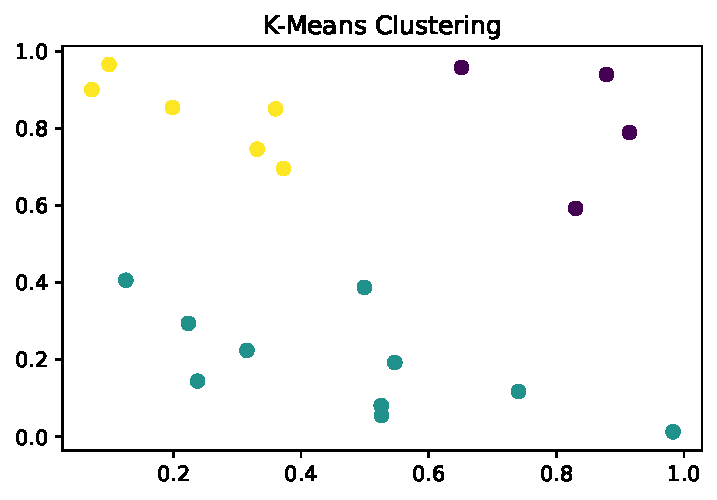
\includegraphics[keepaspectratio]{course/chapters/SEDA/AdvancedAnalysis_files/figure-pdf/cell-10-output-1.pdf}}

\begin{itemize}
\tightlist
\item
  \textbf{Hierarchical Clustering:} Builds a tree of clusters using
  agglomerating or divisive methods.
\end{itemize}

\begin{Shaded}
\begin{Highlighting}[]
\ImportTok{import}\NormalTok{ numpy }\ImportTok{as}\NormalTok{ np}
\ImportTok{import}\NormalTok{ matplotlib.pyplot }\ImportTok{as}\NormalTok{ plt}
\ImportTok{from}\NormalTok{ sklearn.cluster }\ImportTok{import}\NormalTok{ AgglomerativeClustering}

\CommentTok{\# Example dataset}
\NormalTok{X }\OperatorTok{=}\NormalTok{ np.random.rand(}\DecValTok{20}\NormalTok{, }\DecValTok{2}\NormalTok{)}
\NormalTok{agg }\OperatorTok{=}\NormalTok{ AgglomerativeClustering(n\_clusters}\OperatorTok{=}\DecValTok{3}\NormalTok{)}
\NormalTok{labels }\OperatorTok{=}\NormalTok{ agg.fit\_predict(X)}

\CommentTok{\# Plot Clusters}
\NormalTok{plt.scatter(X[:, }\DecValTok{0}\NormalTok{], X[:, }\DecValTok{1}\NormalTok{], c}\OperatorTok{=}\NormalTok{labels, cmap}\OperatorTok{=}\StringTok{\textquotesingle{}viridis\textquotesingle{}}\NormalTok{)}
\NormalTok{plt.title(}\StringTok{\textquotesingle{}Hierarchical Clustering\textquotesingle{}}\NormalTok{)}
\NormalTok{plt.show()}
\end{Highlighting}
\end{Shaded}

\pandocbounded{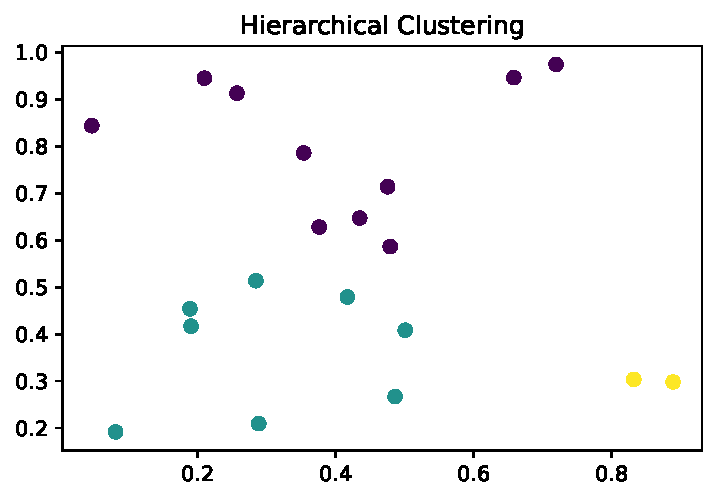
\includegraphics[keepaspectratio]{course/chapters/SEDA/AdvancedAnalysis_files/figure-pdf/cell-11-output-1.pdf}}

\part{Exercises}

\chapter{Exercise A 2}\label{exercise-a-2}

\section{Temperature in Synthesis Reactor Part
2}\label{temperature-in-synthesis-reactor-part-2}

In this exercise, we will repeat not-linear fits.

Let's analyze how bad the situation is in reactor 3 is. To do this, we
will fit a sigmoid curve to the data set. Try to remember which kind of
function we used to fit the non-linear data in the lecture.

In our case the sigmoid function is given by:

\[
T(t) = T_0 + \Delta T \frac{1}{1 + e^{-a (t - t_0)}}
\]

with the four fitting parameters being:

\begin{itemize}
\tightlist
\item
  temperature baseline \$T\_0 \$,
\item
  the temperature increase \(\Delta T\),
\item
  the growth rate \(a\),
\item
  the time at the midpoint of the temperature increase \(t_0\)
\end{itemize}

Use your results from Part 1 of this exercise.

\subsection{Task 1:}\label{task-1}

\begin{itemize}
\tightlist
\item
  Fit a sigmoid function to the data set of reactor 3.
\item
  Plot the data and the fitted curve.
\end{itemize}

\subsection{Questions:}\label{questions-1}

\begin{itemize}
\tightlist
\item
  How much is the tempearture changed in reactor 3?
\item
  How fast this change appears?
\item
  When does the temperature reach the midpoint of the change?
\end{itemize}

\subsection{Task2:}\label{task2}

\begin{itemize}
\tightlist
\item
  Fit a suitable distribution function over the histograms plots of the
  temperature data
\end{itemize}

\subsection{Questions:}\label{questions-2}

\begin{itemize}
\tightlist
\item
  What can you say about the distribution of the temperature data?
\end{itemize}

\chapter{Exercise B 1}\label{exercise-b-1}

\chapter{Exercise:}\label{exercise-1}

\section{Linear Regression: Calibration IR
spectroscopy}\label{linear-regression-calibration-ir-spectroscopy}

In this exercise, we will repeat linear regressions.

\begin{itemize}
\item
  We will learn how to use \texttt{np.polyfit} to perform linear
  regression.
\item
  We will learn how to use \texttt{scipy.stats.linregress} to perform
  linear regression.
\item
  We will learn how to use
  \texttt{sklearn.linear\_model.LinearRegression} to perform linear
  regression.
\item
  We learn what are the differences between these three methods.
\item
  We will learn how to use the linear regression to calculate the
  concentration of a unknown sample.
\end{itemize}

In quantitative spectroscopy we measure the (dimensionless) absorbance
\(A\) of a beam of light at a selected frequency/wavelength to determine
the concentration \(c\) of a sample. To do this, we first calibrate the
device using solutions with known concentration.

\subsection{Data}\label{data-1}

In our exercise we compare the calibrations of two groups of students
available in the files \texttt{ir\_spectroscopy1.dat} and
\texttt{ir\_spectroscopy2.dat}.

\subsection{Data Path:}\label{data-path-1}

\begin{Shaded}
\begin{Highlighting}[]
\NormalTok{data\_path }\OperatorTok{=} \StringTok{"https://raw.githubusercontent.com/stkroe/PythonForChemists/main/course/data/exercises/Linear\_regression/"}
\end{Highlighting}
\end{Shaded}

\subsection{Task}\label{task-2}

\begin{itemize}
\tightlist
\item
  Load the data from the files \texttt{ir\_spectroscopy1.dat} and
  \texttt{ir\_spectroscopy2.dat}.
\item
  Perform a linear regression on the data of each group.
\item
  Compare the results of the three methods.
\item
  Use the linear regression to predict the concentration of our unknown
  sample measured at the absorption of \(A_\mathrm{sample} = 0.753\).
\end{itemize}

\subsection{Questions}\label{questions-3}

\begin{itemize}
\tightlist
\item
  What is the concentration of the unknown sample?
\item
  Are the differences between the three methods?
\item
  Which method would you recommend for this type of data?
\end{itemize}

\chapter{Exercise B 2}\label{exercise-b-2}

\chapter{Exercise:}\label{exercise-2}

\section{Linear Regression and Correlation: Experimental vs.~Theoretical
Data}\label{linear-regression-and-correlation-experimental-vs.-theoretical-data}

In this exercise, we will repeat linear regressions and use it for
demonstration of the correlation between experimental and theoretical
data.

\begin{itemize}
\tightlist
\item
  We will learn how to use create symmetrical plots.
\item
  We will learn to use z-scores outlier test.
\end{itemize}

In this exercise we compare experimentally measured electrochemical
potentials of anthraquinone (AQ) derivatives with those calculated using
theoretical methods. We want to find out how well the calculation can
reproduce the experimental data. And check if there are any outliers in
the data.

\href{https://en.wikipedia.org/wiki/Anthraquinone}{Anthraquinone} is an
aromatic organic molecule, with manifold applications. In nature, AQ and
its derivatives are found in plants and microorganisms due to its key
role in reversible redox reactions. For this reason AQ derivates are
also key components in industrial processes and material development
(\href{https://www.uibk.ac.at/de/physchem/forschung/batterietechnologien/}{such
as battery research at the University of Innsbruck}).

\subsection{Data}\label{data-2}

The data for this exercise is taken from a recent collaboration between
the Theoretical Chemistry Department and the Institute for Physical
chemistry.
(\href{https://pubs.rsc.org/en/content/articlehtml/2022/cp/d2cp01717b}{Phys.Chem.Chem.Phys.
2022, \textbf{24}, \emph{16207 -- 16219}}~).

The experimental data is stored in the file \texttt{experimental.dat}
and the theoretical data is stored in the file \texttt{theory.dat}.

The data contains the following columns:

\begin{itemize}
\tightlist
\item
  \texttt{1-OH} : the name of the AQ derivative
\item
  \texttt{-530.0} : the first redox potential in V
\item
  \texttt{-1178.5}: the second redox potential in V
\end{itemize}

\subsection{Data Path:}\label{data-path-2}

https://raw.githubusercontent.com/stkroe/PythonForChemists/main/course/data/exercises/Anthraquinone/

\subsection{Task}\label{task-3}

\begin{itemize}
\tightlist
\item
  Load the data from the files \texttt{experimental.dat} and
  \texttt{theory.dat}.
\item
  Have fist a look at the data.
\item
  Create a correlation plot of the experimental and theoretical data.
\item
  Perform a linear regression of the data.
\item
  Calculate the correlation coefficient.
\item
  Check for outliers in the data using the z-scores method.
\end{itemize}

\subsection{Questions}\label{questions-4}

\begin{itemize}
\tightlist
\item
  How well do the theoretical data reproduce the experimental data?
\item
  Are there any outliers in the data?
\end{itemize}

\chapter{Exercise B 3}\label{exercise-b-3}

\chapter{Exercise:}\label{exercise-3}

\section{Arrhenious Plot}\label{arrhenious-plot}

In this exercise, we will repeat linear regressions and how to use the
logarithm of the

\begin{itemize}
\tightlist
\item
  We will learn how to use create \texttt{np.log}.
\item
  We will learn how to select a specific range of data.
\item
  We will learn how to use \texttt{scipy.linregress} to perform linear
  regression.
\end{itemize}

\section{Exercise B.3 -- Arrhenius Curve
Fitting}\label{exercise-b.3-arrhenius-curve-fitting}

In this exercise we have a look at diffusion data (either from
experiment or theoretical calculations) and want to obtain the
activation energy \(E_A\).

Many dynamical properties in chemistry (such as rate constants,
diffusion, etc.) follow an
\href{https://en.wikipedia.org/wiki/Arrhenius_plot}{Arrhenian
temperature dependency} given as

\[ y(T) = y_0 e^{-\frac{E_A}{RT}} \]

with \(y_0\) being the pre-exponential factor, R and T are the molar gas
constant (8.3145 J mol\(^{-1}\) K \(^{-1}\)) and temperature,
respectively.

One potential option to obtain \(E_A\) is a non-linear exponential fit,
but this is known to be less reliable than its linear counterpart!

Consequently,
Mr.~\href{https://en.wikipedia.org/wiki/Svante_Arrhenius}{Svante
Arrhenius} used a linearization of the equation, which in case of the
diffusion coefficient looks like this:

\[ ln(D) = ln(D_0) - \frac{E_A}{R}\frac{1}{T} \]

This corresponds to a linear equation

\[ y = a\cdot x + b\]

\[y = ln(D)\]

\[ x= \frac{1}{T}\]

Applying standard linear regression we obtain

\[a=ln(D_0)\] \[b = -\frac{E_A}{R}\]

From this we can directly access the activation energy \(E_A\) via:
\[ E_A = - a \cdot R \]

Easy! :D

This time the files are in
\href{https://en.wikipedia.org/wiki/Comma-separated_values}{csv-format}
(= comma separated values), \emph{i.e.} the different data columns are
separated by comma symbols.

Luckily, we can again use the command \emph{np.loadtext()}, but we have
to indicate the comma by adding \emph{delimiter = ``,''}.

Most programs such as Excel, Origin and scientific software can write
data sets in this format. If you want to use python in your research,
this is most likely the most common file format to input you data sets.

\subsection{Data}\label{data-3}

We have three data sets with diffusion coefficients \(D\) in nm \(^2\)
/ps at different temperatures \(T\) in K.

\begin{itemize}
\tightlist
\item
  \texttt{D\_vs\_T\_v1.csv} (Diffusion coefficient vs.~temperature)
\item
  \texttt{D\_vs\_T\_v2.csv} (Diffusion coefficient vs.~temperature)
\item
  \texttt{D\_vs\_T\_v3.csv} (Diffusion coefficient vs.~temperature)
\end{itemize}

\subsection{Data Path:}\label{data-path-3}

https://raw.githubusercontent.com/stkroe/PythonForChemists/main/course/data/exercises/Arrhenius/

\subsection{Task}\label{task-4}

\begin{itemize}
\tightlist
\item
  Load the data from the files \texttt{D\_vs\_T\_v1.csv},
  \texttt{D\_vs\_T\_v2.csv} and \texttt{D\_vs\_T\_v3.csv} into numpy
  arrays.
\item
  Create a plot of the diffusion coefficient \(D\) vs.~temperature
  \(T\).
\item
  Create a plot of the logarithm of the diffusion coefficient \(ln(D)\)
  vs.~\(1/T\).
\item
  Perform a linear regression of the data using
  \texttt{scipy.stats.linregress} only in the linear region of the data.
\item
  Calculate the activation energy \(E_A\) from the slope of the linear
  regression.
\end{itemize}

\subsection{Questions}\label{questions-5}

\begin{itemize}
\tightlist
\item
  Which data set has the highest activation energy?
\end{itemize}

\part{Data Visualization 2}

\chapter{Advanced Plot Types}\label{advanced-plot-types}

Difficulty level: { }

\begin{itemize}
\tightlist
\item
  \href{https://networkx.org/documentation/stable/auto_examples/index.html}{Network
  plot}: It is used to show the relationship between different nodes. It
  is used to show the relationship between different entities
  \emph{e.g.} protein-protein interaction network
  \href{http://www.ncbi.nlm.nih.gov/pmc/articles/pmc4017556/}{PPI}.
\end{itemize}

\section{Multiple Correlation
Analysis}\label{multiple-correlation-analysis}

\begin{Shaded}
\begin{Highlighting}[]
\ImportTok{import}\NormalTok{ numpy }\ImportTok{as}\NormalTok{ np}
\ImportTok{import}\NormalTok{ seaborn }\ImportTok{as}\NormalTok{ sns}
\ImportTok{import}\NormalTok{ matplotlib.pyplot }\ImportTok{as}\NormalTok{ plt}
\ImportTok{import}\NormalTok{ pandas }\ImportTok{as}\NormalTok{ pd}

\NormalTok{rs }\OperatorTok{=}\NormalTok{ np.random.RandomState(}\DecValTok{33}\NormalTok{)}
\NormalTok{df }\OperatorTok{=}\NormalTok{ pd.DataFrame(data}\OperatorTok{=}\NormalTok{rs.normal(size}\OperatorTok{=}\NormalTok{(}\DecValTok{100}\NormalTok{, }\DecValTok{4}\NormalTok{)), columns}\OperatorTok{=}\NormalTok{[}\StringTok{\textquotesingle{}A\textquotesingle{}}\NormalTok{, }\StringTok{\textquotesingle{}B\textquotesingle{}}\NormalTok{, }\StringTok{\textquotesingle{}C\textquotesingle{}}\NormalTok{, }\StringTok{\textquotesingle{}D\textquotesingle{}}\NormalTok{])}


\CommentTok{\# Compute correlation matrix}
\NormalTok{corr\_matrix }\OperatorTok{=}\NormalTok{ df.corr()}

\CommentTok{\# Visualizing with a heatmap}
\NormalTok{sns.heatmap(corr\_matrix, annot}\OperatorTok{=}\VariableTok{True}\NormalTok{, cmap}\OperatorTok{=}\StringTok{"coolwarm"}\NormalTok{)}

\NormalTok{plt.show()}
\end{Highlighting}
\end{Shaded}

\pandocbounded{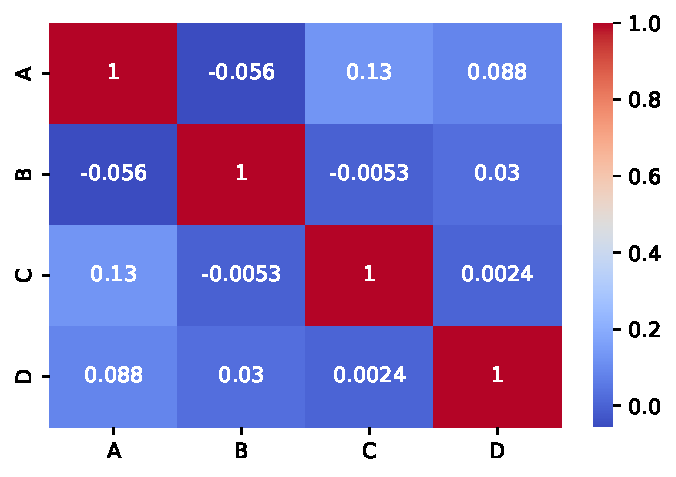
\includegraphics[keepaspectratio]{course/chapters/PlotTypes/AdvancedPlotTypes_files/figure-pdf/cell-2-output-1.pdf}}

\section{PCA Plot}\label{pca-plot}

\begin{Shaded}
\begin{Highlighting}[]
\ImportTok{import}\NormalTok{ numpy }\ImportTok{as}\NormalTok{ np}
\ImportTok{import}\NormalTok{ matplotlib.pyplot }\ImportTok{as}\NormalTok{ plt}
\ImportTok{from}\NormalTok{ sklearn.decomposition }\ImportTok{import}\NormalTok{ PCA}
\ImportTok{from}\NormalTok{ sklearn.preprocessing }\ImportTok{import}\NormalTok{ StandardScaler}

\CommentTok{\# Sample dataset}
\NormalTok{X }\OperatorTok{=}\NormalTok{ np.random.rand(}\DecValTok{10}\NormalTok{, }\DecValTok{3}\NormalTok{)}

\CommentTok{\# Standardizing Data}
\NormalTok{scaler }\OperatorTok{=}\NormalTok{ StandardScaler()}

\NormalTok{X\_scaled }\OperatorTok{=}\NormalTok{ scaler.fit\_transform(X)}

\CommentTok{\# Applying PCA}
\NormalTok{pca }\OperatorTok{=}\NormalTok{ PCA(n\_components}\OperatorTok{=}\DecValTok{2}\NormalTok{)}
\NormalTok{X\_pca }\OperatorTok{=}\NormalTok{ pca.fit\_transform(X\_scaled)}

\CommentTok{\# Plot PCA results}
\NormalTok{plt.scatter(X\_pca[:, }\DecValTok{0}\NormalTok{], X\_pca[:, }\DecValTok{1}\NormalTok{])}
\NormalTok{plt.xlabel(}\StringTok{\textquotesingle{}PC1\textquotesingle{}}\NormalTok{)}
\NormalTok{plt.ylabel(}\StringTok{\textquotesingle{}PC2\textquotesingle{}}\NormalTok{)}
\NormalTok{plt.title(}\StringTok{\textquotesingle{}PCA Analysis\textquotesingle{}}\NormalTok{)}
\NormalTok{plt.show()}
\end{Highlighting}
\end{Shaded}

\pandocbounded{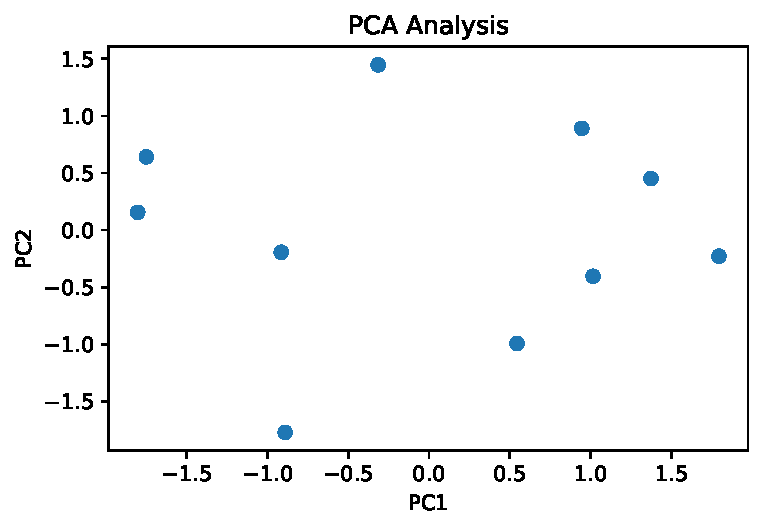
\includegraphics[keepaspectratio]{course/chapters/PlotTypes/AdvancedPlotTypes_files/figure-pdf/cell-3-output-1.pdf}}

\section{Network Plot}\label{network-plot}

\begin{Shaded}
\begin{Highlighting}[]
\ImportTok{import}\NormalTok{ networkx }\ImportTok{as}\NormalTok{ nx}
\ImportTok{import}\NormalTok{ matplotlib.pyplot }\ImportTok{as}\NormalTok{ plt}

\NormalTok{G }\OperatorTok{=}\NormalTok{ nx.Graph()}
\NormalTok{G.add\_node(}\DecValTok{1}\NormalTok{)}
\NormalTok{G.add\_nodes\_from([}\DecValTok{2}\NormalTok{, }\DecValTok{3}\NormalTok{])}
\NormalTok{G.add\_edge(}\DecValTok{1}\NormalTok{, }\DecValTok{2}\NormalTok{)}
\NormalTok{G.add\_edges\_from([(}\DecValTok{1}\NormalTok{, }\DecValTok{2}\NormalTok{), (}\DecValTok{1}\NormalTok{, }\DecValTok{3}\NormalTok{)])}
\NormalTok{nx.draw(G, with\_labels}\OperatorTok{=}\VariableTok{True}\NormalTok{)}
\NormalTok{plt.show()}
\end{Highlighting}
\end{Shaded}

\pandocbounded{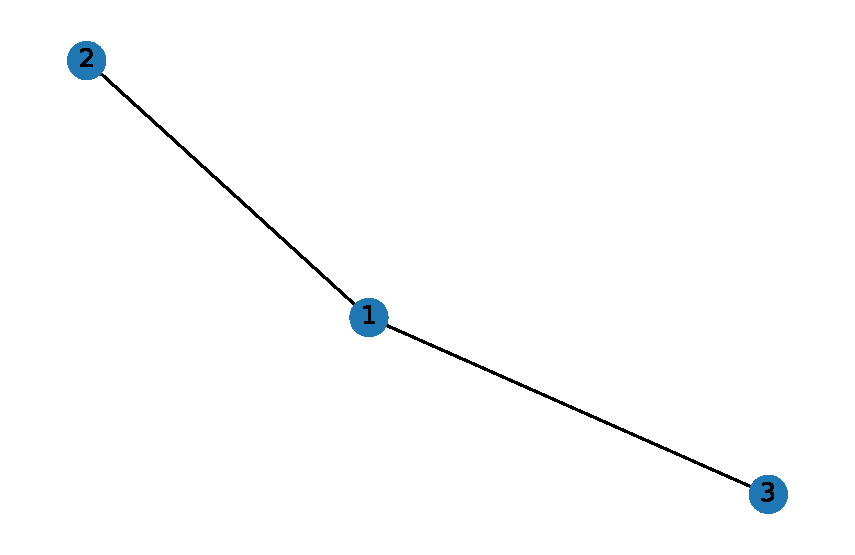
\includegraphics[keepaspectratio]{course/chapters/PlotTypes/AdvancedPlotTypes_files/figure-pdf/cell-4-output-1.pdf}}

\begin{center}\rule{0.5\linewidth}{0.5pt}\end{center}

\section{3D Plot}\label{d-plot}

\begin{Shaded}
\begin{Highlighting}[]
\ImportTok{import}\NormalTok{ numpy }\ImportTok{as}\NormalTok{ np}
\ImportTok{import}\NormalTok{ matplotlib.pyplot }\ImportTok{as}\NormalTok{ plt}
\ImportTok{from}\NormalTok{ mpl\_toolkits.mplot3d }\ImportTok{import}\NormalTok{ Axes3D}

\NormalTok{x }\OperatorTok{=}\NormalTok{ np.linspace(}\OperatorTok{{-}}\DecValTok{5}\NormalTok{, }\DecValTok{5}\NormalTok{, }\DecValTok{100}\NormalTok{) }
\NormalTok{y }\OperatorTok{=}\NormalTok{ np.linspace(}\OperatorTok{{-}}\DecValTok{5}\NormalTok{, }\DecValTok{5}\NormalTok{, }\DecValTok{100}\NormalTok{)}
\NormalTok{X, Y }\OperatorTok{=}\NormalTok{ np.meshgrid(x, y)}
\NormalTok{Z }\OperatorTok{=}\NormalTok{ np.sin(np.sqrt(X}\OperatorTok{**}\DecValTok{2} \OperatorTok{+}\NormalTok{ Y}\OperatorTok{**}\DecValTok{2}\NormalTok{))}

\NormalTok{fig }\OperatorTok{=}\NormalTok{ plt.figure()}
\NormalTok{ax }\OperatorTok{=}\NormalTok{ fig.add\_subplot(}\DecValTok{111}\NormalTok{, projection}\OperatorTok{=}\StringTok{\textquotesingle{}3d\textquotesingle{}}\NormalTok{)}
\NormalTok{ax.plot\_surface(X, Y, Z)}
\NormalTok{plt.show()}
\end{Highlighting}
\end{Shaded}

\pandocbounded{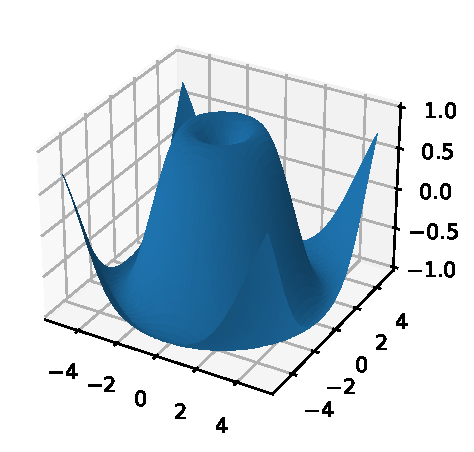
\includegraphics[keepaspectratio]{course/chapters/PlotTypes/AdvancedPlotTypes_files/figure-pdf/cell-5-output-1.pdf}}

\chapter{Interactive Plots}\label{interactive-plots}

Difficulty level: { }

\section*{Interactive Plots}\label{interactive-plots-1}
\addcontentsline{toc}{section}{Interactive Plots}

\markright{Interactive Plots}

\subsection*{Matplotlib and ipywidget}\label{matplotlib-and-ipywidget}
\addcontentsline{toc}{subsection}{Matplotlib and ipywidget}

\begin{Shaded}
\begin{Highlighting}[]
\ImportTok{from}\NormalTok{ matplotlib }\ImportTok{import}\NormalTok{ pyplot }\ImportTok{as}\NormalTok{ plt}
\ImportTok{import}\NormalTok{ numpy }\ImportTok{as}\NormalTok{ np}
\ImportTok{import}\NormalTok{ ipywidgets }\ImportTok{as}\NormalTok{ widgets}
\ImportTok{from}\NormalTok{ IPython.display }\ImportTok{import}\NormalTok{ display}

\NormalTok{x }\OperatorTok{=}\NormalTok{ np.linspace(}\DecValTok{0}\NormalTok{, }\DecValTok{10}\NormalTok{, }\DecValTok{100}\NormalTok{)}
\NormalTok{y }\OperatorTok{=}\NormalTok{ np.sin(x)}

\KeywordTok{def}\NormalTok{ plot\_sine(frequency):}
\NormalTok{    plt.plot(x, np.sin(frequency}\OperatorTok{*}\NormalTok{x))}
\NormalTok{    plt.show()}
  
\NormalTok{frequency\_slider }\OperatorTok{=}\NormalTok{ widgets.FloatSlider(value}\OperatorTok{=}\DecValTok{1}\NormalTok{, }\BuiltInTok{min}\OperatorTok{=}\FloatTok{0.1}\NormalTok{, }\BuiltInTok{max}\OperatorTok{=}\DecValTok{10}\NormalTok{, step}\OperatorTok{=}\FloatTok{0.1}\NormalTok{)}
\NormalTok{widgets.interactive(plot\_sine, frequency}\OperatorTok{=}\NormalTok{frequency\_slider)}
\end{Highlighting}
\end{Shaded}

\begin{verbatim}
interactive(children=(FloatSlider(value=1.0, description='frequency', max=10.0, min=0.1), Output()), _dom_clas…
\end{verbatim}

\begin{center}\rule{0.5\linewidth}{0.5pt}\end{center}

\subsection*{Plotly}\label{plotly}
\addcontentsline{toc}{subsection}{Plotly}

Ploty is a library that allows you to create interactive plots and
dashboards, see the \href{https://plotly.com/graphing-libraries/}{Plotly
website}.

\begin{Shaded}
\begin{Highlighting}[]
\ImportTok{import}\NormalTok{ plotly.express }\ImportTok{as}\NormalTok{ px}
\ImportTok{import}\NormalTok{ numpy }\ImportTok{as}\NormalTok{ np}

\NormalTok{x }\OperatorTok{=}\NormalTok{ np.linspace(}\DecValTok{0}\NormalTok{, }\DecValTok{10}\NormalTok{, }\DecValTok{100}\NormalTok{)}
\NormalTok{y }\OperatorTok{=}\NormalTok{ np.sin(x)}

\NormalTok{fig }\OperatorTok{=}\NormalTok{ px.line(x}\OperatorTok{=}\NormalTok{x, y}\OperatorTok{=}\NormalTok{y, title}\OperatorTok{=}\StringTok{\textquotesingle{}Sine function\textquotesingle{}}\NormalTok{)}
\NormalTok{fig.show()}
\end{Highlighting}
\end{Shaded}

\begin{verbatim}
Unable to display output for mime type(s): text/html
\end{verbatim}

\begin{verbatim}
Unable to display output for mime type(s): text/html
\end{verbatim}

\begin{center}\rule{0.5\linewidth}{0.5pt}\end{center}

\subsection*{Bokeh}\label{bokeh}
\addcontentsline{toc}{subsection}{Bokeh}

Bokeh is a library that allows you to create interactive plots and
dashboards, see the
\href{https://docs.bokeh.org/en/latest/index.html}{Bokeh website}.

\begin{Shaded}
\begin{Highlighting}[]
\ImportTok{from}\NormalTok{ bokeh.plotting }\ImportTok{import}\NormalTok{ figure, show}
\ImportTok{from}\NormalTok{ bokeh.io }\ImportTok{import}\NormalTok{ output\_notebook}
\ImportTok{import}\NormalTok{ numpy }\ImportTok{as}\NormalTok{ np}

\NormalTok{output\_notebook()}

\NormalTok{x }\OperatorTok{=}\NormalTok{ np.linspace(}\DecValTok{0}\NormalTok{, }\DecValTok{10}\NormalTok{, }\DecValTok{100}\NormalTok{)}
\NormalTok{y }\OperatorTok{=}\NormalTok{ np.sin(x)}

\NormalTok{p }\OperatorTok{=}\NormalTok{ figure(title}\OperatorTok{=}\StringTok{\textquotesingle{}Sine function\textquotesingle{}}\NormalTok{)}
\NormalTok{p.line(x, y)}
\NormalTok{show(p)}
\end{Highlighting}
\end{Shaded}

\begin{verbatim}
Unable to display output for mime type(s): text/html
\end{verbatim}

\begin{verbatim}
Unable to display output for mime type(s): application/javascript, application/vnd.bokehjs_load.v0+json
\end{verbatim}

\begin{verbatim}
Unable to display output for mime type(s): text/html
\end{verbatim}

\begin{verbatim}
Unable to display output for mime type(s): application/javascript, application/vnd.bokehjs_exec.v0+json
\end{verbatim}

\begin{center}\rule{0.5\linewidth}{0.5pt}\end{center}

\subsection*{Altair}\label{altair}
\addcontentsline{toc}{subsection}{Altair}

Altair is a library that allows you to create interactive plots and
dashboards, see the \href{https://altair-viz.github.io/}{Altair
website}.

\begin{Shaded}
\begin{Highlighting}[]
\ImportTok{import}\NormalTok{ altair }\ImportTok{as}\NormalTok{ alt}
\ImportTok{import}\NormalTok{ pandas }\ImportTok{as}\NormalTok{ pd}
\ImportTok{import}\NormalTok{ numpy }\ImportTok{as}\NormalTok{ np}

\NormalTok{x }\OperatorTok{=}\NormalTok{ np.linspace(}\DecValTok{0}\NormalTok{, }\DecValTok{10}\NormalTok{, }\DecValTok{100}\NormalTok{)}
\NormalTok{y }\OperatorTok{=}\NormalTok{ np.sin(x)}

\NormalTok{df }\OperatorTok{=}\NormalTok{ pd.DataFrame(\{}\StringTok{\textquotesingle{}x\textquotesingle{}}\NormalTok{: x, }\StringTok{\textquotesingle{}y\textquotesingle{}}\NormalTok{: y\})}

\NormalTok{alt.Chart(df).mark\_line().encode(}
\NormalTok{    x}\OperatorTok{=}\StringTok{\textquotesingle{}x\textquotesingle{}}\NormalTok{,}
\NormalTok{    y}\OperatorTok{=}\StringTok{\textquotesingle{}y\textquotesingle{}}
\NormalTok{).properties(}
\NormalTok{    title}\OperatorTok{=}\StringTok{\textquotesingle{}Sine function\textquotesingle{}}
\NormalTok{)}
\end{Highlighting}
\end{Shaded}

\begin{verbatim}
alt.Chart(...)
\end{verbatim}

\part{Exercises}

\chapter{Exercise D 1}\label{exercise-d-1}

\chapter{Exercise:}\label{exercise-4}

\section{3D Plot}\label{d-plot-1}

In this exercise, we will repeat to plot the 3D data.

\subsection{Data}\label{data-4}

The 3D data is given in the file \texttt{grid\_data.dat}. The data
contains the following columns: - \(r_\mathrm{OH_1}\) distance from O to
H1 atom in Angstrom - \(r_\mathrm{OH_2}\) distance from O to H2 atom in
Angstrom - \(V\) potential energy in kcal/mol

\subsection{Data Path:}\label{data-path-4}

\begin{Shaded}
\begin{Highlighting}[]
\NormalTok{data\_path }\OperatorTok{=} \StringTok{"https://raw.githubusercontent.com/stkroe/PythonForChemists/main/course/data/exercises/3D\_data/"}
\end{Highlighting}
\end{Shaded}

\subsection{Task}\label{task-5}

\begin{itemize}
\tightlist
\item
  Load the data from the files \texttt{grid\_data.dat}.
\item
  Create a 3D plot of the data using the \texttt{plot\_surface}
  function.
\item
  Use a meaningful color map.
\end{itemize}

\chapter{Exercise D 2}\label{exercise-d-2}

\chapter{Exercise:}\label{exercise-5}

\section{Interactive Plot}\label{interactive-plot}

In this exercise, we will repeat how to create an interactive plot using
\texttt{ipywidgets}.

\subsection{Task 1}\label{task-1-1}

\begin{itemize}
\tightlist
\item
  Create an interactive plot using \texttt{ipywidgets} and
  \texttt{matplotlib} for the van-Deemeter equation where the user can
  change the parameters \(a\), \(b\) and \(c\) using sliders.
\end{itemize}

\subsection{Task 1}\label{task-1-2}

\begin{itemize}
\tightlist
\item
  Create an interactive plot using \texttt{ipywidgets} and
  \texttt{matplotlib} for a rate equation together with an Arrhenius
  Plot where the user can change the parameters \(k_0\),and \(E_a\)
  using sliders.
\end{itemize}

\part{Special Analysis and Visualization Techniques}

\chapter{Analysis of Spectroscopy
Data}\label{analysis-of-spectroscopy-data}

Difficulty level: { }

\section*{Spectroscopy Data Analysis}\label{spectroscopy-data-analysis}
\addcontentsline{toc}{section}{Spectroscopy Data Analysis}

\markright{Spectroscopy Data Analysis}

Spectroscopy is one of the most used experimental techniques in
chemistry \emph{e.g.}:

\begin{itemize}
\tightlist
\item
  UV/Vis spectroscopy
\item
  IR spectroscopy
\item
  NMR spectroscopy
\item
  Mass spectroscopy
\end{itemize}

The analysis of spectroscopy needs often some preprocessing steps
\emph{e.g.}:

\begin{itemize}
\tightlist
\item
  Baseline correction
\item
  Smoothing
\item
  Normalization
\item
  Peak assignment
\item
  Peak fitting
\item
  Peak integration
\item
  Peak deconvolution
\end{itemize}

\subsection*{Feature Detection}\label{feature-detection}
\addcontentsline{toc}{subsection}{Feature Detection}

In spectroscopy data, peaks are often the most important features.

Maxima and minima are often used to identify the peaks in the data.

Global maxima and minima can be found using the \texttt{min} and
\texttt{max}, \texttt{np.min} and \texttt{np.max} or
\texttt{df{[}\textquotesingle{}column\_name\textquotesingle{}{]}.min()}
and
\texttt{df{[}\textquotesingle{}column\_name\textquotesingle{}{]}.max()}
functions.

Local maxima and minima can be found also by using the
\texttt{argrelextrema} function from the \texttt{scipy.signal} module.

\begin{Shaded}
\begin{Highlighting}[]
\ImportTok{import}\NormalTok{ numpy }\ImportTok{as}\NormalTok{ np}
\ImportTok{from}\NormalTok{ scipy.signal }\ImportTok{import}\NormalTok{ argrelextrema}
\ImportTok{import}\NormalTok{ matplotlib.pyplot }\ImportTok{as}\NormalTok{ plt}

\CommentTok{\# Generate some data transmission data}
\NormalTok{x }\OperatorTok{=}\NormalTok{ np.linspace(}\DecValTok{0}\NormalTok{, }\DecValTok{10}\NormalTok{, }\DecValTok{100}\NormalTok{)}
\NormalTok{y }\OperatorTok{=}\NormalTok{ np.sin(x) }\OperatorTok{+}\NormalTok{ np.random.normal(}\DecValTok{0}\NormalTok{, }\FloatTok{0.1}\NormalTok{, x.size)}
\NormalTok{y[}\DecValTok{30}\NormalTok{:}\DecValTok{40}\NormalTok{] }\OperatorTok{=}\NormalTok{ np.exp(}\OperatorTok{{-}}\NormalTok{y[}\DecValTok{30}\NormalTok{:}\DecValTok{40}\NormalTok{]) }\OperatorTok{+} \FloatTok{0.5}

\CommentTok{\# Find local maxima and minima}
\NormalTok{local\_max }\OperatorTok{=}\NormalTok{ argrelextrema(y, np.greater,order}\OperatorTok{=}\DecValTok{200}\NormalTok{)[}\DecValTok{0}\NormalTok{]}
\NormalTok{local\_min }\OperatorTok{=}\NormalTok{ argrelextrema(y, np.less)[}\DecValTok{0}\NormalTok{]}

\CommentTok{\# Plot the data}
\NormalTok{plt.plot(x, y, label}\OperatorTok{=}\StringTok{\textquotesingle{}Data\textquotesingle{}}\NormalTok{)}
\NormalTok{plt.plot(x[local\_min], y[local\_min], }\StringTok{\textquotesingle{}o\textquotesingle{}}\NormalTok{, color}\OperatorTok{=}\StringTok{\textquotesingle{}green\textquotesingle{}}\NormalTok{, label}\OperatorTok{=}\StringTok{\textquotesingle{}Local Minima\textquotesingle{}}\NormalTok{)}
\NormalTok{plt.scatter(x[local\_max], y[local\_max], color}\OperatorTok{=}\StringTok{\textquotesingle{}red\textquotesingle{}}\NormalTok{, label}\OperatorTok{=}\StringTok{\textquotesingle{}Local Maxima\textquotesingle{}}\NormalTok{)}
\NormalTok{plt.ylabel(}\StringTok{\textquotesingle{}Y{-}axis\textquotesingle{}}\NormalTok{)}
\NormalTok{plt.xlabel(}\StringTok{\textquotesingle{}X{-}axis\textquotesingle{}}\NormalTok{)}
\NormalTok{plt.title(}\StringTok{\textquotesingle{}Local Maxima and Minima\textquotesingle{}}\NormalTok{)}

\NormalTok{plt.legend()}

\NormalTok{plt.show()}
\end{Highlighting}
\end{Shaded}

\pandocbounded{\includegraphics[keepaspectratio]{course/chapters/SpecialAnalysisPlots/Spectroscopy_files/figure-pdf/cell-2-output-1.pdf}}

\texttt{find\_peaks} function from the \texttt{scipy.signal} module can
be used to find the peaks in the data. It finds the local maxima in the
data and returns the indices of the peaks. If you want to find the
minima, you can simply invert the data by multiplying it with -1.

\begin{Shaded}
\begin{Highlighting}[]
\ImportTok{import}\NormalTok{ numpy }\ImportTok{as}\NormalTok{ np}
\ImportTok{import}\NormalTok{ matplotlib.pyplot }\ImportTok{as}\NormalTok{ plt}
\ImportTok{from}\NormalTok{ scipy.signal }\ImportTok{import}\NormalTok{ find\_peaks}

\CommentTok{\# Generate some data}
\NormalTok{x }\OperatorTok{=}\NormalTok{ np.linspace(}\DecValTok{0}\NormalTok{, }\DecValTok{10}\NormalTok{, }\DecValTok{100}\NormalTok{)}
\NormalTok{y }\OperatorTok{=}\NormalTok{ np.sin(x) }\OperatorTok{+}\NormalTok{ np.random.normal(}\DecValTok{0}\NormalTok{, }\FloatTok{0.1}\NormalTok{, x.size)}
\NormalTok{y[}\DecValTok{30}\NormalTok{:}\DecValTok{40}\NormalTok{] }\OperatorTok{=}\NormalTok{ np.exp(}\OperatorTok{{-}}\NormalTok{y[}\DecValTok{30}\NormalTok{:}\DecValTok{40}\NormalTok{]) }\OperatorTok{+} \FloatTok{0.5}
\CommentTok{\# Find peaks}
\NormalTok{peaks, \_ }\OperatorTok{=}\NormalTok{ find\_peaks(y, height}\OperatorTok{=}\FloatTok{0.5}\NormalTok{, distance}\OperatorTok{=}\DecValTok{10}\NormalTok{)}
\CommentTok{\# Plot the data}
\NormalTok{plt.plot(x, y, label}\OperatorTok{=}\StringTok{\textquotesingle{}Data\textquotesingle{}}\NormalTok{)}
\NormalTok{plt.plot(x[peaks], y[peaks], }\StringTok{\textquotesingle{}o\textquotesingle{}}\NormalTok{, color}\OperatorTok{=}\StringTok{\textquotesingle{}red\textquotesingle{}}\NormalTok{, label}\OperatorTok{=}\StringTok{\textquotesingle{}Peaks\textquotesingle{}}\NormalTok{)}
\NormalTok{plt.ylabel(}\StringTok{\textquotesingle{}Y{-}axis\textquotesingle{}}\NormalTok{)}
\NormalTok{plt.xlabel(}\StringTok{\textquotesingle{}X{-}axis\textquotesingle{}}\NormalTok{)}
\NormalTok{plt.title(}\StringTok{\textquotesingle{}Peaks in Data\textquotesingle{}}\NormalTok{)}
\NormalTok{plt.legend()}
\NormalTok{plt.show()}
\end{Highlighting}
\end{Shaded}

\pandocbounded{\includegraphics[keepaspectratio]{course/chapters/SpecialAnalysisPlots/Spectroscopy_files/figure-pdf/cell-3-output-1.pdf}}

You can also use the \texttt{height}, \texttt{threshold},
\texttt{distance}, \texttt{prominence} and \texttt{width} parameters to
filter the peaks to enhance the peak detection.

\begin{itemize}
\tightlist
\item
  \texttt{height}: Minimum height of the peaks
\item
  \texttt{threshold}: Minimum vertical distance to its neighboring
  samples
\item
  \texttt{distance}: Minimum horizontal distance (in samples) between
  neighboring peaks
\item
  \texttt{prominence}: Minimum prominence of the peaks
\end{itemize}

\begin{Shaded}
\begin{Highlighting}[]
\ImportTok{import}\NormalTok{ numpy }\ImportTok{as}\NormalTok{ np}
\ImportTok{import}\NormalTok{ matplotlib.pyplot }\ImportTok{as}\NormalTok{ plt}
\ImportTok{from}\NormalTok{ scipy.signal }\ImportTok{import}\NormalTok{ find\_peaks}

\CommentTok{\# Generate some data}
\NormalTok{x }\OperatorTok{=}\NormalTok{ np.linspace(}\DecValTok{0}\NormalTok{, }\DecValTok{10}\NormalTok{, }\DecValTok{100}\NormalTok{)}
\NormalTok{y }\OperatorTok{=}\NormalTok{ np.sin(x) }\OperatorTok{+}\NormalTok{ np.random.normal(}\DecValTok{0}\NormalTok{, }\FloatTok{0.1}\NormalTok{, x.size)}
\NormalTok{y[}\DecValTok{30}\NormalTok{:}\DecValTok{40}\NormalTok{] }\OperatorTok{=}\NormalTok{ np.exp(}\OperatorTok{{-}}\NormalTok{y[}\DecValTok{30}\NormalTok{:}\DecValTok{40}\NormalTok{]) }\OperatorTok{+} \FloatTok{0.5}
\CommentTok{\# Find peaks}
\NormalTok{peaks, \_ }\OperatorTok{=}\NormalTok{ find\_peaks(y, height}\OperatorTok{=}\FloatTok{0.5}\NormalTok{, distance}\OperatorTok{=}\DecValTok{10}\NormalTok{, prominence}\OperatorTok{=}\FloatTok{0.5}\NormalTok{, width}\OperatorTok{=}\DecValTok{1}\NormalTok{)}
\CommentTok{\# Plot the data}
\NormalTok{plt.plot(x, y, label}\OperatorTok{=}\StringTok{\textquotesingle{}Data\textquotesingle{}}\NormalTok{)    }
\NormalTok{plt.plot(x[peaks], y[peaks], }\StringTok{\textquotesingle{}o\textquotesingle{}}\NormalTok{, color}\OperatorTok{=}\StringTok{\textquotesingle{}red\textquotesingle{}}\NormalTok{, label}\OperatorTok{=}\StringTok{\textquotesingle{}Peaks\textquotesingle{}}\NormalTok{)}
\NormalTok{plt.ylabel(}\StringTok{\textquotesingle{}Y{-}axis\textquotesingle{}}\NormalTok{)}
\NormalTok{plt.xlabel(}\StringTok{\textquotesingle{}X{-}axis\textquotesingle{}}\NormalTok{)}
\NormalTok{plt.title(}\StringTok{\textquotesingle{}Peaks in Data\textquotesingle{}}\NormalTok{)}
\NormalTok{plt.legend()}
\NormalTok{plt.show()}
\end{Highlighting}
\end{Shaded}

\pandocbounded{\includegraphics[keepaspectratio]{course/chapters/SpecialAnalysisPlots/Spectroscopy_files/figure-pdf/cell-4-output-1.pdf}}

\subsection*{Smoothing}\label{smoothing}
\addcontentsline{toc}{subsection}{Smoothing}

Often data is noisy and needs to be smoothed before further analysis.

\begin{itemize}
\tightlist
\item
  Moving average
\item
  Weighted moving average
\item
  Gaussian filter
\item
  Savitzky-Golay filter
\end{itemize}

\textbf{Moving Average}

\begin{Shaded}
\begin{Highlighting}[]
\ImportTok{import}\NormalTok{ numpy }\ImportTok{as}\NormalTok{ np}
\ImportTok{import}\NormalTok{ matplotlib.pyplot }\ImportTok{as}\NormalTok{ plt}


\CommentTok{\# Generate some data}
\NormalTok{x }\OperatorTok{=}\NormalTok{ np.linspace(}\DecValTok{0}\NormalTok{, }\DecValTok{10}\NormalTok{, }\DecValTok{100}\NormalTok{)}
\NormalTok{y }\OperatorTok{=}\NormalTok{ np.sin(x) }\OperatorTok{+}\NormalTok{ np.random.normal(}\DecValTok{0}\NormalTok{, }\FloatTok{0.1}\NormalTok{, x.size)}

\CommentTok{\# Apply the moving average}
\NormalTok{window\_size }\OperatorTok{=} \DecValTok{5}

\NormalTok{smoothed\_data }\OperatorTok{=}\NormalTok{np.convolve(y, np.ones(window\_size)}\OperatorTok{/}\NormalTok{window\_size, mode}\OperatorTok{=}\StringTok{\textquotesingle{}same\textquotesingle{}}\NormalTok{)}

\CommentTok{\# Plot the data}
\NormalTok{plt.plot(x, y, label}\OperatorTok{=}\StringTok{\textquotesingle{}Data\textquotesingle{}}\NormalTok{)}
\NormalTok{plt.plot(x, smoothed\_data, label}\OperatorTok{=}\StringTok{\textquotesingle{}Smoothed Data\textquotesingle{}}\NormalTok{, color}\OperatorTok{=}\StringTok{\textquotesingle{}red\textquotesingle{}}\NormalTok{)}
\NormalTok{plt.ylabel(}\StringTok{\textquotesingle{}Y{-}axis\textquotesingle{}}\NormalTok{)}
\NormalTok{plt.xlabel(}\StringTok{\textquotesingle{}X{-}axis\textquotesingle{}}\NormalTok{)}
\NormalTok{plt.title(}\StringTok{\textquotesingle{}Moving Average\textquotesingle{}}\NormalTok{)}
\NormalTok{plt.legend()}
\NormalTok{plt.show()}
\end{Highlighting}
\end{Shaded}

\pandocbounded{\includegraphics[keepaspectratio]{course/chapters/SpecialAnalysisPlots/Spectroscopy_files/figure-pdf/cell-5-output-1.pdf}}

\textbf{Gaussian Filter}

\begin{Shaded}
\begin{Highlighting}[]
\ImportTok{import}\NormalTok{ numpy }\ImportTok{as}\NormalTok{ np}
\ImportTok{import}\NormalTok{ matplotlib.pyplot }\ImportTok{as}\NormalTok{ plt}
\ImportTok{from}\NormalTok{ scipy.ndimage }\ImportTok{import}\NormalTok{ gaussian\_filter1d}
\CommentTok{\# Generate some data}
\NormalTok{x }\OperatorTok{=}\NormalTok{ np.linspace(}\DecValTok{0}\NormalTok{, }\DecValTok{10}\NormalTok{, }\DecValTok{100}\NormalTok{)}
\NormalTok{y }\OperatorTok{=}\NormalTok{ np.sin(x) }\OperatorTok{+}\NormalTok{ np.random.normal(}\DecValTok{0}\NormalTok{, }\FloatTok{0.1}\NormalTok{, x.size)}
\CommentTok{\# Apply the Gaussian filter}
\NormalTok{sigma }\OperatorTok{=} \DecValTok{2}
\NormalTok{smoothed\_data }\OperatorTok{=}\NormalTok{ gaussian\_filter1d(y, sigma}\OperatorTok{=}\NormalTok{sigma)}
\CommentTok{\# Plot the data}
\NormalTok{plt.plot(x, y, label}\OperatorTok{=}\StringTok{\textquotesingle{}Data\textquotesingle{}}\NormalTok{)}

\NormalTok{plt.plot(x, smoothed\_data, label}\OperatorTok{=}\StringTok{\textquotesingle{}Smoothed Data\textquotesingle{}}\NormalTok{, color}\OperatorTok{=}\StringTok{\textquotesingle{}red\textquotesingle{}}\NormalTok{)}
\NormalTok{plt.ylabel(}\StringTok{\textquotesingle{}Y{-}axis\textquotesingle{}}\NormalTok{)}
\NormalTok{plt.xlabel(}\StringTok{\textquotesingle{}X{-}axis\textquotesingle{}}\NormalTok{)}
\NormalTok{plt.title(}\StringTok{\textquotesingle{}Gaussian Filter\textquotesingle{}}\NormalTok{)}
\NormalTok{plt.legend()}
\NormalTok{plt.show()}
\end{Highlighting}
\end{Shaded}

\pandocbounded{\includegraphics[keepaspectratio]{course/chapters/SpecialAnalysisPlots/Spectroscopy_files/figure-pdf/cell-6-output-1.pdf}}

\textbf{Savitzky-Golay Filter}

\begin{Shaded}
\begin{Highlighting}[]
\ImportTok{import}\NormalTok{ numpy }\ImportTok{as}\NormalTok{ np}
\ImportTok{import}\NormalTok{ matplotlib.pyplot }\ImportTok{as}\NormalTok{ plt}
\ImportTok{from}\NormalTok{ scipy.signal }\ImportTok{import}\NormalTok{ savgol\_filter}
\CommentTok{\# Generate some data}
\NormalTok{x }\OperatorTok{=}\NormalTok{ np.linspace(}\DecValTok{0}\NormalTok{, }\DecValTok{10}\NormalTok{, }\DecValTok{100}\NormalTok{)}
\NormalTok{y }\OperatorTok{=}\NormalTok{ np.sin(x) }\OperatorTok{+}\NormalTok{ np.random.normal(}\DecValTok{0}\NormalTok{, }\FloatTok{0.1}\NormalTok{, x.size)}
\CommentTok{\# Apply the Savitzky{-}Golay filter}
\NormalTok{window\_size }\OperatorTok{=} \DecValTok{5}
\NormalTok{poly\_order }\OperatorTok{=} \DecValTok{2}
\NormalTok{smoothed\_data }\OperatorTok{=}\NormalTok{ savgol\_filter(y, window\_size, poly\_order)}
\CommentTok{\# Plot the data}
\NormalTok{plt.plot(x, y, label}\OperatorTok{=}\StringTok{\textquotesingle{}Data\textquotesingle{}}\NormalTok{)}
\NormalTok{plt.plot(x, smoothed\_data, label}\OperatorTok{=}\StringTok{\textquotesingle{}Smoothed Data\textquotesingle{}}\NormalTok{, color}\OperatorTok{=}\StringTok{\textquotesingle{}red\textquotesingle{}}\NormalTok{)}
\NormalTok{plt.ylabel(}\StringTok{\textquotesingle{}Y{-}axis\textquotesingle{}}\NormalTok{)}
\NormalTok{plt.xlabel(}\StringTok{\textquotesingle{}X{-}axis\textquotesingle{}}\NormalTok{)}
\NormalTok{plt.title(}\StringTok{\textquotesingle{}Savitzky{-}Golay Filter\textquotesingle{}}\NormalTok{)}
\NormalTok{plt.legend()}
\NormalTok{plt.show()}
\end{Highlighting}
\end{Shaded}

\pandocbounded{\includegraphics[keepaspectratio]{course/chapters/SpecialAnalysisPlots/Spectroscopy_files/figure-pdf/cell-7-output-1.pdf}}

\subsection*{Baseline Correction}\label{baseline-correction}
\addcontentsline{toc}{subsection}{Baseline Correction}

A baseline correction is often needed to remove background noise from
the signal and

The baseline correction can be done by different methods \emph{e.g.}:

\begin{itemize}
\tightlist
\item
  Polynomial fitting
\item
  Spline fitting
\item
  Minimum value fitting
\item
  Moving average etc.
\end{itemize}

There exists also a package called
\href{https://pybaselines.readthedocs.io/en/latest/}{\texttt{pybaselines}}
which can be used to correct the baseline of the data.

\begin{Shaded}
\begin{Highlighting}[]
\OperatorTok{!}\NormalTok{pip install pybaselines}
\end{Highlighting}
\end{Shaded}

\begin{verbatim}
Requirement already satisfied: pybaselines in /Users/stk/y/envs/myenv/lib/python3.12/site-packages (1.2.0)
Requirement already satisfied: numpy>=1.20 in /Users/stk/y/envs/myenv/lib/python3.12/site-packages (from pybaselines) (2.0.0)
Requirement already satisfied: scipy>=1.6 in /Users/stk/y/envs/myenv/lib/python3.12/site-packages (from pybaselines) (1.15.2)
\end{verbatim}

\begin{Shaded}
\begin{Highlighting}[]
\ImportTok{import}\NormalTok{ numpy }\ImportTok{as}\NormalTok{ np}
\ImportTok{import}\NormalTok{ matplotlib.pyplot }\ImportTok{as}\NormalTok{ plt}
\ImportTok{from}\NormalTok{ scipy.ndimage }\ImportTok{import}\NormalTok{ gaussian\_filter1d}
\ImportTok{from}\NormalTok{ pybaselines }\ImportTok{import}\NormalTok{ Baseline}
\ImportTok{from}\NormalTok{ pybaselines.utils }\ImportTok{import}\NormalTok{ gaussian}


\CommentTok{\# Generate some data}
\NormalTok{x }\OperatorTok{=}\NormalTok{ np.linspace(}\DecValTok{20}\NormalTok{, }\DecValTok{1000}\NormalTok{, }\DecValTok{1000}\NormalTok{)}
\NormalTok{signal }\OperatorTok{=}\NormalTok{ (}
    \OperatorTok{+}\NormalTok{ gaussian(x, }\DecValTok{6}\NormalTok{, }\DecValTok{240}\NormalTok{, }\DecValTok{5}\NormalTok{)}
    \OperatorTok{+}\NormalTok{ gaussian(x, }\DecValTok{8}\NormalTok{, }\DecValTok{350}\NormalTok{, }\DecValTok{11}\NormalTok{)}
    \OperatorTok{+}\NormalTok{ gaussian(x, }\DecValTok{15}\NormalTok{, }\DecValTok{400}\NormalTok{, }\DecValTok{18}\NormalTok{)}
    \OperatorTok{+}\NormalTok{ gaussian(x, }\DecValTok{6}\NormalTok{, }\DecValTok{550}\NormalTok{, }\DecValTok{6}\NormalTok{)}
    \OperatorTok{+}\NormalTok{ gaussian(x, }\DecValTok{13}\NormalTok{, }\DecValTok{700}\NormalTok{, }\DecValTok{8}\NormalTok{)}
    \OperatorTok{+}\NormalTok{ gaussian(x, }\DecValTok{9}\NormalTok{, }\DecValTok{800}\NormalTok{, }\DecValTok{9}\NormalTok{)}
    \OperatorTok{+}\NormalTok{ gaussian(x, }\DecValTok{9}\NormalTok{, }\DecValTok{880}\NormalTok{, }\DecValTok{7}\NormalTok{)}
\NormalTok{)}
\NormalTok{baseline }\OperatorTok{=} \DecValTok{5} \OperatorTok{+} \DecValTok{6} \OperatorTok{*}\NormalTok{ np.exp(}\OperatorTok{{-}}\NormalTok{(x }\OperatorTok{{-}} \DecValTok{40}\NormalTok{) }\OperatorTok{/} \DecValTok{30}\NormalTok{) }\OperatorTok{+}\NormalTok{ gaussian(x, }\DecValTok{5}\NormalTok{, }\DecValTok{1000}\NormalTok{, }\DecValTok{300}\NormalTok{)}
\NormalTok{noise }\OperatorTok{=}\NormalTok{ np.random.default\_rng(}\DecValTok{0}\NormalTok{).normal(}\DecValTok{0}\NormalTok{, }\FloatTok{0.1}\NormalTok{, }\BuiltInTok{len}\NormalTok{(x))}
\NormalTok{y }\OperatorTok{=}\NormalTok{ signal }\OperatorTok{+}\NormalTok{ baseline }\OperatorTok{+}\NormalTok{ noise}

\CommentTok{\# Use the Baseline class to fit the baseline}
\NormalTok{baseline\_fitter }\OperatorTok{=}\NormalTok{ Baseline(x\_data}\OperatorTok{=}\NormalTok{x)}
\CommentTok{\# The baseline\_fitter object can be used to fit the baseline with different methods in that case the Asymmetrically Reweighted Penalized Least Squares (ARPLS)}
\NormalTok{stiff\_baseline }\OperatorTok{=}\NormalTok{ baseline\_fitter.arpls(y, lam}\OperatorTok{=}\FloatTok{5e5}\NormalTok{)[}\DecValTok{0}\NormalTok{]}
\CommentTok{\# Correct the data by subtracting the baseline}
\NormalTok{data\_corrected }\OperatorTok{=}\NormalTok{ y }\OperatorTok{{-}}\NormalTok{ stiff\_baseline}

\CommentTok{\# Create subplots}
\NormalTok{fig, axs }\OperatorTok{=}\NormalTok{ plt.subplots(}\DecValTok{3}\NormalTok{, }\DecValTok{1}\NormalTok{, figsize}\OperatorTok{=}\NormalTok{(}\DecValTok{8}\NormalTok{, }\DecValTok{12}\NormalTok{))}
\NormalTok{axs[}\DecValTok{0}\NormalTok{].plot(x, y, label}\OperatorTok{=}\StringTok{\textquotesingle{}Data\textquotesingle{}}\NormalTok{)}
\NormalTok{axs[}\DecValTok{0}\NormalTok{].plot(x, signal, label}\OperatorTok{=}\StringTok{\textquotesingle{}Signal\textquotesingle{}}\NormalTok{)}
\NormalTok{axs[}\DecValTok{0}\NormalTok{].plot(x, baseline, label}\OperatorTok{=}\StringTok{\textquotesingle{}Baseline\textquotesingle{}}\NormalTok{)}
\NormalTok{axs[}\DecValTok{0}\NormalTok{].set\_ylabel(}\StringTok{\textquotesingle{}Y{-}axis\textquotesingle{}}\NormalTok{)}
\NormalTok{axs[}\DecValTok{0}\NormalTok{].set\_xlabel(}\StringTok{\textquotesingle{}X{-}axis\textquotesingle{}}\NormalTok{)}
\NormalTok{axs[}\DecValTok{0}\NormalTok{].set\_title(}\StringTok{\textquotesingle{}Data with Baseline\textquotesingle{}}\NormalTok{)}
\NormalTok{axs[}\DecValTok{0}\NormalTok{].legend()}
\NormalTok{axs[}\DecValTok{1}\NormalTok{].plot(x, y, label}\OperatorTok{=}\StringTok{\textquotesingle{}Data\textquotesingle{}}\NormalTok{)}
\NormalTok{axs[}\DecValTok{1}\NormalTok{].plot(x, stiff\_baseline, label}\OperatorTok{=}\StringTok{\textquotesingle{}Stiff Baseline\textquotesingle{}}\NormalTok{)}
\NormalTok{axs[}\DecValTok{1}\NormalTok{].set\_ylabel(}\StringTok{\textquotesingle{}Y{-}axis\textquotesingle{}}\NormalTok{)}
\NormalTok{axs[}\DecValTok{1}\NormalTok{].set\_xlabel(}\StringTok{\textquotesingle{}X{-}axis\textquotesingle{}}\NormalTok{)}
\NormalTok{axs[}\DecValTok{1}\NormalTok{].set\_title(}\StringTok{\textquotesingle{}Stiff Baseline\textquotesingle{}}\NormalTok{)}
\NormalTok{axs[}\DecValTok{1}\NormalTok{].legend()}
\NormalTok{axs[}\DecValTok{2}\NormalTok{].plot(x, y, label}\OperatorTok{=}\StringTok{\textquotesingle{}Data\textquotesingle{}}\NormalTok{)}
\NormalTok{axs[}\DecValTok{2}\NormalTok{].plot(x, data\_corrected, label}\OperatorTok{=}\StringTok{\textquotesingle{}Corrected Data\textquotesingle{}}\NormalTok{)}
\NormalTok{axs[}\DecValTok{2}\NormalTok{].set\_ylabel(}\StringTok{\textquotesingle{}Y{-}axis\textquotesingle{}}\NormalTok{)}
\NormalTok{axs[}\DecValTok{2}\NormalTok{].set\_xlabel(}\StringTok{\textquotesingle{}X{-}axis\textquotesingle{}}\NormalTok{)}
\NormalTok{axs[}\DecValTok{2}\NormalTok{].set\_title(}\StringTok{\textquotesingle{}Corrected Data\textquotesingle{}}\NormalTok{)}
\NormalTok{axs[}\DecValTok{2}\NormalTok{].legend()}
\NormalTok{plt.tight\_layout()}
\NormalTok{plt.show()}
\end{Highlighting}
\end{Shaded}

\pandocbounded{\includegraphics[keepaspectratio]{course/chapters/SpecialAnalysisPlots/Spectroscopy_files/figure-pdf/cell-9-output-1.pdf}}

\chapter{Analysis of Image Data}\label{analysis-of-image-data}

Difficulty level: { }

\section*{Image Data Analysis}\label{image-data-analysis}
\addcontentsline{toc}{section}{Image Data Analysis}

\markright{Image Data Analysis}

\chapter{Ternary Plot}\label{ternary-plot}

Difficulty level: { }

\chapter*{Ternary Plot}\label{ternary-plot-1}
\addcontentsline{toc}{chapter}{Ternary Plot}

\markboth{Ternary Plot}{Ternary Plot}

A ternary plot is a type of plot that is used to visualize the
composition of three components.

\begin{Shaded}
\begin{Highlighting}[]
\ImportTok{import}\NormalTok{ matplotlib.pyplot }\ImportTok{as}\NormalTok{ plt}
\ImportTok{import}\NormalTok{ numpy }\ImportTok{as}\NormalTok{ np}
\ImportTok{import}\NormalTok{ ternary}

\CommentTok{\# Create a figure}
\NormalTok{fig, tax }\OperatorTok{=}\NormalTok{ ternary.figure(scale}\OperatorTok{=}\FloatTok{1.0}\NormalTok{)}

\CommentTok{\# Draw Boundary and Gridlines}
\NormalTok{tax.boundary(linewidth}\OperatorTok{=}\FloatTok{2.0}\NormalTok{)}
\NormalTok{tax.gridlines(multiple}\OperatorTok{=}\FloatTok{0.2}\NormalTok{, color}\OperatorTok{=}\StringTok{"blue"}\NormalTok{)}

\CommentTok{\# Set Axis labels and Title}
\NormalTok{fontsize }\OperatorTok{=} \DecValTok{10}
\NormalTok{tax.set\_title(}\StringTok{"Ternary Plot"}\NormalTok{, fontsize}\OperatorTok{=}\NormalTok{fontsize)}
\NormalTok{tax.left\_axis\_label(}\StringTok{"Component A"}\NormalTok{, fontsize}\OperatorTok{=}\NormalTok{fontsize)}
\NormalTok{tax.right\_axis\_label(}\StringTok{"Component B"}\NormalTok{, fontsize}\OperatorTok{=}\NormalTok{fontsize)}
\NormalTok{tax.bottom\_axis\_label(}\StringTok{"Component C"}\NormalTok{, fontsize}\OperatorTok{=}\NormalTok{fontsize)}

\CommentTok{\# Plot some data}
\NormalTok{points }\OperatorTok{=}\NormalTok{ np.random.dirichlet((}\DecValTok{1}\NormalTok{, }\DecValTok{1}\NormalTok{, }\DecValTok{1}\NormalTok{), }\DecValTok{10}\NormalTok{)}
\NormalTok{tax.scatter(points, marker}\OperatorTok{=}\StringTok{\textquotesingle{}s\textquotesingle{}}\NormalTok{, color}\OperatorTok{=}\StringTok{\textquotesingle{}red\textquotesingle{}}\NormalTok{, label}\OperatorTok{=}\StringTok{"Data"}\NormalTok{)}

\CommentTok{\# Legend}
\NormalTok{tax.legend()}
\NormalTok{plt.show()}
\end{Highlighting}
\end{Shaded}

\pandocbounded{\includegraphics[keepaspectratio]{course/chapters/SpecialAnalysisPlots/Ternary_files/figure-pdf/cell-2-output-1.pdf}}

\part{Exercises}

\chapter{Exercise C 1}\label{exercise-c-1}

\chapter{Exercise:}\label{exercise-6}

\section{Spectroscopic data analysis}\label{spectroscopic-data-analysis}

In this exercise, we will repeat how spectroscopic data can be analyzed
effectively via Python \texttt{SciPy}library.

\begin{itemize}
\tightlist
\item
  We will learn denoising and smoothing of data (SM).
\item
  We will learn how to correct the baseline of data (BC).
\item
  We will learn how to detect peaks in data (PD).
\end{itemize}

These kind of analysis methods can be relevant when depicting X-ray
diffraction patterns, spectrograms obtained from various techniques
(e.g.~IR/Raman, UV/Vis, X-ray, NMR, \ldots), chromatograms and
electropherograms and many more.

Often the experimental data is subject to noise or has a notable offset
in the baseline.

\texttt{SciPy} offers a number of straightforward tools to quickly
enhance the data to make it ready for plotting.

Let's start by reading in some X-ray diffraction data.

\subsection{Data}\label{data-5}

The data is a simple X-ray diffraction pattern of a crystalline
material. The experimental data is stored in
\texttt{XRD\_experimental.dat}and the theoretical data in
\texttt{XRD\_theory.dat}.

First column represents the 2-theta angle in degrees, the second column
represents the intensity in arbitrary units.

\subsection{Data Path:}\label{data-path-5}

\begin{Shaded}
\begin{Highlighting}[]
\NormalTok{data\_path }\OperatorTok{=} \StringTok{\textquotesingle{}https://raw.githubusercontent.com/stkroe/PythonForChemists/main/course/data/exercises/X{-}ray\_Diffraction/\textquotesingle{}}
\end{Highlighting}
\end{Shaded}

\subsection{Task}\label{task-6}

\begin{itemize}
\tightlist
\item
  Load the data from the files \texttt{XRD\_experimental.dat} and
  \texttt{XRD\_theory.dat}.
\item
  Have fist a look at the data.
\item
  Normalize the data to the maximum intensity to 100.
\item
  Smooth the experimental data using a Gaussian filter with a standard
  deviation of 2.0.
\item
  Find the peaks in the experimental data using the \texttt{find\_peaks}
  function from \texttt{scipy.signal}.
\item
  Plot the smoothed experimental data.
\item
  Add a baseline correction to the experimental data using the
  \texttt{minimum\_fiter1d} function from \texttt{scipy.ndimage}.
\item
  Plot the baseline corrected experimental data.
\item
  Find the peaks in the baseline corrected data uing the
  \texttt{find\_peaks} function from \texttt{scipy.signal}.
\item
  Compare the smoothed experimental data with the smoothed and baseline
  corrected experimental data via a correlation plot and linear
  regression.
\item
  Compare both experimental smoothed and baseline corrected data and
  theoretical data via a correlation plot and linear regression.
\end{itemize}

\subsection{Questions}\label{questions-6}

\begin{itemize}
\tightlist
\item
  What effect does the Gaussian filter have on the data?
\item
  How does the baseline correction affect the data?
\item
  How well does the smoothed data correlate with the theoretical data?
\end{itemize}

\chapter{Exercise C 2}\label{exercise-c-2}

\chapter{Exercise:}\label{exercise-7}

\section{Chromotography and Spectroscopy
Integration}\label{chromotography-and-spectroscopy-integration}

In this exercise, we will repeat how spectroscopic data can be
integrated via Python \texttt{SciPy}library.

\begin{itemize}
\tightlist
\item
  We will learn denoising and smoothing of data (SM).
\item
  We will learn how to correct the baseline of data (BC).
\item
  We will learn how to detect peaks in data (PD).
\item
  We will learn how to integrate the area under the curve (AUC).
\end{itemize}

In this example we are using the featues of \texttt{finde-peaks()} to
determine the left and right integration limits to integrate peaks of an
example chromatogram.

To achieve this, we first have to reduce the noise and apply a baseline
correction.

Let's start by loading the file!

\subsection{Data}\label{data-6}

The chromatographic data is stored in a file called
\texttt{Chromatogram.csv}.

First column represents the time in min and the second column represents
the intensity in arbitrary units (a.u.).

\subsection{Data Path:}\label{data-path-6}

\begin{Shaded}
\begin{Highlighting}[]
\NormalTok{data\_path }\OperatorTok{=} \StringTok{"https://raw.githubusercontent.com/stkroe/PythonForChemists/main/course/data/exercises/Chromatography/"}
\end{Highlighting}
\end{Shaded}

\subsection{Task}\label{task-7}

\begin{itemize}
\tightlist
\item
  Load the data from the files \texttt{Chromatogram.csv}.
\item
  Apply Gaussian smoothing and minimum filtered baseline correction.
\item
  Detect the peaks and integrate the area under the curve.
\item
  Plot the chromatogram with the detected peaks and the integrated area
  under the curve.
\end{itemize}

\subsection{Questions}\label{questions-7}

\begin{itemize}
\tightlist
\item
  What is the area under the curve for each peak?
\end{itemize}

\part{Playground}

\chapter{Exercise Playground}\label{exercise-playground}

\chapter{Playground for Python}\label{playground-for-python}

You can use the \texttt{load\_wine} dataset from the \texttt{sklearn}
library to practice data manipulation and visualization. Below is a code
snippet that demonstrates how to load the dataset, perform some basic
data analysis, and visualize it using \texttt{matplotlib}.

\begin{Shaded}
\begin{Highlighting}[]
\ImportTok{import}\NormalTok{ pandas }\ImportTok{as}\NormalTok{ pd}
\ImportTok{import}\NormalTok{ matplotlib.pyplot }\ImportTok{as}\NormalTok{ plt}
\ImportTok{from}\NormalTok{ sklearn.datasets }\ImportTok{import}\NormalTok{ load\_wine}
\end{Highlighting}
\end{Shaded}

The \texttt{load\_wine} dataset contains information about different
types of wines, including their chemical properties and quality ratings.
You can use this dataset to practice various data manipulation
techniques, such as filtering, grouping, and aggregating data.

\begin{Shaded}
\begin{Highlighting}[]
\NormalTok{data }\OperatorTok{=}\NormalTok{ load\_wine()}
\NormalTok{data}
\end{Highlighting}
\end{Shaded}

\begin{verbatim}
{'data': array([[1.423e+01, 1.710e+00, 2.430e+00, ..., 1.040e+00, 3.920e+00,
         1.065e+03],
        [1.320e+01, 1.780e+00, 2.140e+00, ..., 1.050e+00, 3.400e+00,
         1.050e+03],
        [1.316e+01, 2.360e+00, 2.670e+00, ..., 1.030e+00, 3.170e+00,
         1.185e+03],
        ...,
        [1.327e+01, 4.280e+00, 2.260e+00, ..., 5.900e-01, 1.560e+00,
         8.350e+02],
        [1.317e+01, 2.590e+00, 2.370e+00, ..., 6.000e-01, 1.620e+00,
         8.400e+02],
        [1.413e+01, 4.100e+00, 2.740e+00, ..., 6.100e-01, 1.600e+00,
         5.600e+02]]),
 'target': array([0, 0, 0, 0, 0, 0, 0, 0, 0, 0, 0, 0, 0, 0, 0, 0, 0, 0, 0, 0, 0, 0,
        0, 0, 0, 0, 0, 0, 0, 0, 0, 0, 0, 0, 0, 0, 0, 0, 0, 0, 0, 0, 0, 0,
        0, 0, 0, 0, 0, 0, 0, 0, 0, 0, 0, 0, 0, 0, 0, 1, 1, 1, 1, 1, 1, 1,
        1, 1, 1, 1, 1, 1, 1, 1, 1, 1, 1, 1, 1, 1, 1, 1, 1, 1, 1, 1, 1, 1,
        1, 1, 1, 1, 1, 1, 1, 1, 1, 1, 1, 1, 1, 1, 1, 1, 1, 1, 1, 1, 1, 1,
        1, 1, 1, 1, 1, 1, 1, 1, 1, 1, 1, 1, 1, 1, 1, 1, 1, 1, 1, 1, 2, 2,
        2, 2, 2, 2, 2, 2, 2, 2, 2, 2, 2, 2, 2, 2, 2, 2, 2, 2, 2, 2, 2, 2,
        2, 2, 2, 2, 2, 2, 2, 2, 2, 2, 2, 2, 2, 2, 2, 2, 2, 2, 2, 2, 2, 2,
        2, 2]),
 'frame': None,
 'target_names': array(['class_0', 'class_1', 'class_2'], dtype='<U7'),
 'DESCR': '.. _wine_dataset:\n\nWine recognition dataset\n------------------------\n\n**Data Set Characteristics:**\n\n:Number of Instances: 178\n:Number of Attributes: 13 numeric, predictive attributes and the class\n:Attribute Information:\n    - Alcohol\n    - Malic acid\n    - Ash\n    - Alcalinity of ash\n    - Magnesium\n    - Total phenols\n    - Flavanoids\n    - Nonflavanoid phenols\n    - Proanthocyanins\n    - Color intensity\n    - Hue\n    - OD280/OD315 of diluted wines\n    - Proline\n    - class:\n        - class_0\n        - class_1\n        - class_2\n\n:Summary Statistics:\n\n============================= ==== ===== ======= =====\n                                Min   Max   Mean     SD\n============================= ==== ===== ======= =====\nAlcohol:                      11.0  14.8    13.0   0.8\nMalic Acid:                   0.74  5.80    2.34  1.12\nAsh:                          1.36  3.23    2.36  0.27\nAlcalinity of Ash:            10.6  30.0    19.5   3.3\nMagnesium:                    70.0 162.0    99.7  14.3\nTotal Phenols:                0.98  3.88    2.29  0.63\nFlavanoids:                   0.34  5.08    2.03  1.00\nNonflavanoid Phenols:         0.13  0.66    0.36  0.12\nProanthocyanins:              0.41  3.58    1.59  0.57\nColour Intensity:              1.3  13.0     5.1   2.3\nHue:                          0.48  1.71    0.96  0.23\nOD280/OD315 of diluted wines: 1.27  4.00    2.61  0.71\nProline:                       278  1680     746   315\n============================= ==== ===== ======= =====\n\n:Missing Attribute Values: None\n:Class Distribution: class_0 (59), class_1 (71), class_2 (48)\n:Creator: R.A. Fisher\n:Donor: Michael Marshall (MARSHALL%PLU@io.arc.nasa.gov)\n:Date: July, 1988\n\nThis is a copy of UCI ML Wine recognition datasets.\nhttps://archive.ics.uci.edu/ml/machine-learning-databases/wine/wine.data\n\nThe data is the results of a chemical analysis of wines grown in the same\nregion in Italy by three different cultivators. There are thirteen different\nmeasurements taken for different constituents found in the three types of\nwine.\n\nOriginal Owners:\n\nForina, M. et al, PARVUS -\nAn Extendible Package for Data Exploration, Classification and Correlation.\nInstitute of Pharmaceutical and Food Analysis and Technologies,\nVia Brigata Salerno, 16147 Genoa, Italy.\n\nCitation:\n\nLichman, M. (2013). UCI Machine Learning Repository\n[https://archive.ics.uci.edu/ml]. Irvine, CA: University of California,\nSchool of Information and Computer Science.\n\n.. dropdown:: References\n\n    (1) S. Aeberhard, D. Coomans and O. de Vel,\n    Comparison of Classifiers in High Dimensional Settings,\n    Tech. Rep. no. 92-02, (1992), Dept. of Computer Science and Dept. of\n    Mathematics and Statistics, James Cook University of North Queensland.\n    (Also submitted to Technometrics).\n\n    The data was used with many others for comparing various\n    classifiers. The classes are separable, though only RDA\n    has achieved 100% correct classification.\n    (RDA : 100%, QDA 99.4%, LDA 98.9%, 1NN 96.1% (z-transformed data))\n    (All results using the leave-one-out technique)\n\n    (2) S. Aeberhard, D. Coomans and O. de Vel,\n    "THE CLASSIFICATION PERFORMANCE OF RDA"\n    Tech. Rep. no. 92-01, (1992), Dept. of Computer Science and Dept. of\n    Mathematics and Statistics, James Cook University of North Queensland.\n    (Also submitted to Journal of Chemometrics).\n',
 'feature_names': ['alcohol',
  'malic_acid',
  'ash',
  'alcalinity_of_ash',
  'magnesium',
  'total_phenols',
  'flavanoids',
  'nonflavanoid_phenols',
  'proanthocyanins',
  'color_intensity',
  'hue',
  'od280/od315_of_diluted_wines',
  'proline']}
\end{verbatim}

\begin{Shaded}
\begin{Highlighting}[]
\NormalTok{df }\OperatorTok{=}\NormalTok{ pd.DataFrame(data.data, columns}\OperatorTok{=}\NormalTok{data.feature\_names)}
\NormalTok{df[}\StringTok{\textquotesingle{}target\textquotesingle{}}\NormalTok{] }\OperatorTok{=}\NormalTok{ data.target}
\NormalTok{df[}\StringTok{\textquotesingle{}targe\_name\textquotesingle{}}\NormalTok{] }\OperatorTok{=}\NormalTok{ df[}\StringTok{\textquotesingle{}target\textquotesingle{}}\NormalTok{].}\BuiltInTok{map}\NormalTok{(\{}\DecValTok{0}\NormalTok{: }\StringTok{\textquotesingle{}Class 0\textquotesingle{}}\NormalTok{, }\DecValTok{1}\NormalTok{: }\StringTok{\textquotesingle{}Class 1\textquotesingle{}}\NormalTok{, }\DecValTok{2}\NormalTok{: }\StringTok{\textquotesingle{}Class 2\textquotesingle{}}\NormalTok{\})}
\NormalTok{df.style }\OperatorTok{\textbackslash{}}
\NormalTok{  .}\BuiltInTok{format}\NormalTok{(precision}\OperatorTok{=}\DecValTok{2}\NormalTok{) }\OperatorTok{\textbackslash{}}
\NormalTok{  .highlight\_max(axis}\OperatorTok{=}\DecValTok{0}\NormalTok{, color}\OperatorTok{=}\StringTok{\textquotesingle{}lightgreen\textquotesingle{}}\NormalTok{) }\OperatorTok{\textbackslash{}}
\NormalTok{  .highlight\_min(axis}\OperatorTok{=}\DecValTok{0}\NormalTok{, color}\OperatorTok{=}\StringTok{\textquotesingle{}lightcoral\textquotesingle{}}\NormalTok{) }\OperatorTok{\textbackslash{}}
\NormalTok{  .set\_caption(}\StringTok{"Wine Dataset Features"}\NormalTok{) }\OperatorTok{\textbackslash{}}
\NormalTok{  .set\_table\_styles(}
\NormalTok{    [\{}\StringTok{\textquotesingle{}selector\textquotesingle{}}\NormalTok{: }\StringTok{\textquotesingle{}th.col0\textquotesingle{}}\NormalTok{, }\StringTok{\textquotesingle{}props\textquotesingle{}}\NormalTok{: [(}\StringTok{\textquotesingle{}color\textquotesingle{}}\NormalTok{, }\StringTok{\textquotesingle{}blue\textquotesingle{}}\NormalTok{), (}\StringTok{\textquotesingle{}font{-}weight\textquotesingle{}}\NormalTok{, }\StringTok{\textquotesingle{}bold\textquotesingle{}}\NormalTok{)]\}]}
\NormalTok{  ) }\OperatorTok{\textbackslash{}}
\NormalTok{  .set\_properties(}\OperatorTok{**}\NormalTok{\{}\StringTok{\textquotesingle{}text{-}align\textquotesingle{}}\NormalTok{: }\StringTok{\textquotesingle{}left\textquotesingle{}}\NormalTok{\}) }\OperatorTok{\textbackslash{}}
\NormalTok{  .set\_table\_attributes(}\StringTok{\textquotesingle{}style="width: 100\%; border: 1px solid black;"\textquotesingle{}}\NormalTok{) }\OperatorTok{\textbackslash{}}
\NormalTok{  .set\_table\_styles(}
\NormalTok{    [\{}\StringTok{\textquotesingle{}selector\textquotesingle{}}\NormalTok{: }\StringTok{\textquotesingle{}th\textquotesingle{}}\NormalTok{, }\StringTok{\textquotesingle{}props\textquotesingle{}}\NormalTok{: [(}\StringTok{\textquotesingle{}background{-}color\textquotesingle{}}\NormalTok{, }\StringTok{\textquotesingle{}\#f2f2f2\textquotesingle{}}\NormalTok{), (}\StringTok{\textquotesingle{}color\textquotesingle{}}\NormalTok{, }\StringTok{\textquotesingle{}black\textquotesingle{}}\NormalTok{)]\}],}
\NormalTok{    axis}\OperatorTok{=}\DecValTok{0}
\NormalTok{  )}
\NormalTok{display(df)}
\end{Highlighting}
\end{Shaded}

\begin{longtable}[]{@{}llllllllllllllll@{}}
\toprule\noalign{}
& alcohol & malic\_acid & ash & alcalinity\_of\_ash & magnesium &
total\_phenols & flavanoids & nonflavanoid\_phenols & proanthocyanins &
color\_intensity & hue & od280/od315\_of\_diluted\_wines & proline &
target & targe\_name \\
\midrule\noalign{}
\endhead
\bottomrule\noalign{}
\endlastfoot
0 & 14.23 & 1.71 & 2.43 & 15.6 & 127.0 & 2.80 & 3.06 & 0.28 & 2.29 &
5.64 & 1.04 & 3.92 & 1065.0 & 0 & Class 0 \\
1 & 13.20 & 1.78 & 2.14 & 11.2 & 100.0 & 2.65 & 2.76 & 0.26 & 1.28 &
4.38 & 1.05 & 3.40 & 1050.0 & 0 & Class 0 \\
2 & 13.16 & 2.36 & 2.67 & 18.6 & 101.0 & 2.80 & 3.24 & 0.30 & 2.81 &
5.68 & 1.03 & 3.17 & 1185.0 & 0 & Class 0 \\
3 & 14.37 & 1.95 & 2.50 & 16.8 & 113.0 & 3.85 & 3.49 & 0.24 & 2.18 &
7.80 & 0.86 & 3.45 & 1480.0 & 0 & Class 0 \\
4 & 13.24 & 2.59 & 2.87 & 21.0 & 118.0 & 2.80 & 2.69 & 0.39 & 1.82 &
4.32 & 1.04 & 2.93 & 735.0 & 0 & Class 0 \\
... & ... & ... & ... & ... & ... & ... & ... & ... & ... & ... & ... &
... & ... & ... & ... \\
173 & 13.71 & 5.65 & 2.45 & 20.5 & 95.0 & 1.68 & 0.61 & 0.52 & 1.06 &
7.70 & 0.64 & 1.74 & 740.0 & 2 & Class 2 \\
174 & 13.40 & 3.91 & 2.48 & 23.0 & 102.0 & 1.80 & 0.75 & 0.43 & 1.41 &
7.30 & 0.70 & 1.56 & 750.0 & 2 & Class 2 \\
175 & 13.27 & 4.28 & 2.26 & 20.0 & 120.0 & 1.59 & 0.69 & 0.43 & 1.35 &
10.20 & 0.59 & 1.56 & 835.0 & 2 & Class 2 \\
176 & 13.17 & 2.59 & 2.37 & 20.0 & 120.0 & 1.65 & 0.68 & 0.53 & 1.46 &
9.30 & 0.60 & 1.62 & 840.0 & 2 & Class 2 \\
177 & 14.13 & 4.10 & 2.74 & 24.5 & 96.0 & 2.05 & 0.76 & 0.56 & 1.35 &
9.20 & 0.61 & 1.60 & 560.0 & 2 & Class 2 \\
\end{longtable}

What you can do with this dataset:

\begin{itemize}
\tightlist
\item
  Load the dataset and explore its structure
\item
  Perform basic data analysis, such as calculating summary statistics
\item
  Visualize the data using different types of plots (e.g., scatter
  plots, histograms)
\end{itemize}

\part{Repetition}

\chapter{Exercise Recap Python}\label{exercise-recap-python}

\subsection{Quiz}\label{quiz-2}

\phantomsection\label{quiz-container}

\section*{Exercise Recap Python}\label{exercise-recap-python-1}
\addcontentsline{toc}{section}{Exercise Recap Python}

\markright{Exercise Recap Python}

Open it locally:

\href{https://github.com/stkroe/PythonforChemists/blob/main/course/exercises/recap_python.ipynb}{Exercise
Recap Python}

Open it in Colab:
\href{https://colab.research.google.com/github/stkroe/PythonForChemists/blob/main/course/exercises/recap_python.ipynb}{Exercise
Recap Python}

\part{Exam}

\chapter{Final Exam}\label{final-exam}

\chapter{1. Temperature vs time plot}\label{temperature-vs-time-plot}

First data set: \texttt{ExamA\_XX.dat}

Temperature in K \textbar{} Time in seconds

\begin{itemize}
\tightlist
\item
  Draw a line plot of the temperature(y-axis) in K vs time(x-axis) in
  hours.
\item
  Calculate the average temperature and the standard deviation. Plot
  both values as horizontal lines in the plot.
\item
  Create a figure which is large enough for publication, label
  everything, and use a suitable font size for the labels, legend,
  x-ticks and y-ticks.
\end{itemize}

\chapter{2. Correlation plot}\label{correlation-plot}

Second data set: \texttt{ExamB\_XX.csv}

Experiment in eV \textbar{} Theory in eV

\begin{itemize}
\tightlist
\item
  Draw a scatter plot of the experimental(y-axis) in eV vs
  theoretical(x-axis) in eV.
\item
  Calculate the correlation coefficient and the linear regression
  parameter.
\item
  Draw the linear regression line in the plot.
\item
  Give the parameters and R \(^2\) of the linear regression line in the
  plot.
\item
  Create a figure which is large enough for publication, label
  everything, and use a suitable font size for the labels, legend,
  x-ticks and y-ticks.
\end{itemize}

\chapter{3. X-ray diffraction plot}\label{x-ray-diffraction-plot}

Third data set: \texttt{ExamC\_XX.csv}

2 \(\theta\) in degrees \textbar{} Intensity in arbitrary units

\begin{itemize}
\tightlist
\item
  Draw a line plot of the intensity(y-axis) in arbitrary units vs 2
  theta(x-axis) in degrees.
\item
  Get the peak positions and draw text boxes with the peak positions in
  the plot.
\item
  Create a figure which is large enough for publication, label
  everything, and use a suitable font size for the labels, legend,
  x-ticks and y-ticks.
\end{itemize}

\part{Informations}

\chapter*{References}\label{references}
\addcontentsline{toc}{chapter}{References}

\markboth{References}{References}

\phantomsection\label{refs}
\begin{CSLReferences}{0}{1}
\end{CSLReferences}

\chapter{License}\label{license}

MIT License

Copyright (c) 2025 Stefanie Kröll and Thomas Hofer

Permission is hereby granted, free of charge, to any person obtaining a
copy of this software and associated documentation files (the
``Software''), to deal in the Software without restriction, including
without limitation the rights to use, copy, modify, merge, publish,
distribute, sublicense, and/or sell copies of the Software, and to
permit persons to whom the Software is furnished to do so, subject to
the following conditions:

The above copyright notice and this permission notice shall be included
in all copies or substantial portions of the Software.

THE SOFTWARE IS PROVIDED ``AS IS'', WITHOUT WARRANTY OF ANY KIND,
EXPRESS OR IMPLIED, INCLUDING BUT NOT LIMITED TO THE WARRANTIES OF
MERCHANTABILITY, FITNESS FOR A PARTICULAR PURPOSE AND NONINFRINGEMENT.
IN NO EVENT SHALL THE AUTHORS OR COPYRIGHT HOLDERS BE LIABLE FOR ANY
CLAIM, DAMAGES OR OTHER LIABILITY, WHETHER IN AN ACTION OF CONTRACT,
TORT OR OTHERWISE, ARISING FROM, OUT OF OR IN CONNECTION WITH THE
SOFTWARE OR THE USE OR OTHER DEALINGS IN THE SOFTWARE.

\chapter{Privacy Policy}\label{privacy-policy}

This website does not collect, store or process any personally
identifiable information and does not use cookies or other tracking
technologies.

\section{Hosting: GitHub Pages}\label{hosting-github-pages}

This website is hosted on \href{https://pages.github.com/}{GitHub
Pages}. GitHub says at

\begin{quote}
Github-Docs \textgreater{} GitHub Pages \textgreater{} Get started
\textgreater{} About GitHub Pages
(\url{https://docs.github.com/en/pages/getting-started-with-github-pages/about-github-pages}):
\end{quote}

\begin{quote}
``When a GitHub Pages site is visited, the visitor's IP address is
logged and stored for security purposes, regardless of whether the
visitor has signed into GitHub or not. For more information about
GitHub's security practices, see
\href{https://docs.github.com/en/site-policy/privacy-policies/github-general-privacy-statemen}{GitHub
Privacy Statement}''
\end{quote}

\chapter{Impressum}\label{impressum}

This Data Analysis and Visualization for Chemists and Material
Scientists tutorial is created by \textbf{Stefanie Kröll, MSc} and a
part of the exercises are created by \textbf{Assoz.-Prof.~Dr.~Thomas
Hofer} as part of the lecture course ``VU Data Science and Visualization
Primer for Chemists and Material Scientists'' at University of
Innsbruck, Austria.

\begin{center}\rule{0.5\linewidth}{0.5pt}\end{center}

\subsection{Contact Information}\label{contact-information}

Write to us if you have any questions or suggestions:

Please contact us via email:

s.kroell@student.uibk.ac.at

\begin{center}\rule{0.5\linewidth}{0.5pt}\end{center}

\begin{itemize}
\tightlist
\item
  \textbf{\href{privacy.qmd}{Privacy Policy}}
\item
  \textbf{\href{disclaimer.qmd}{External Link Policy and Disclaimers}}
\end{itemize}

\subsection{Acknowledgements}\label{acknowledgements}

This tutorial is based on the following sources:

\begin{itemize}
\item
  \href{https://weisscharlesj.github.io/SciCompforChemists/notebooks/introduction/intro.html\#}{Scientific
  Computing for Chemists with Python}
\item
  \href{https://pythoninchemistry.org/intro_python_chemists/intro.html}{An
  introduction to Python for Chemistry}
\end{itemize}

\chapter{Disclaimers}\label{disclaimers}

\textbf{Disclaimer:}\\
All information provided on this website is offered ``as is'' without
any warranties, expressed or implied, including, but not limited to,
warranties of merchantability, fitness for a particular purpose, or
non-infringement. While efforts are made to ensure the accuracy of the
information, the website owner makes no guarantee of its correctness or
completeness. Use the information at your own discretion and risk.

\begin{tcolorbox}[enhanced jigsaw, leftrule=.75mm, bottomrule=.15mm, colbacktitle=quarto-callout-warning-color!10!white, title=\textcolor{quarto-callout-warning-color}{\faExclamationTriangle}\hspace{0.5em}{External Link Policy}, breakable, arc=.35mm, toptitle=1mm, opacityback=0, titlerule=0mm, coltitle=black, colback=white, opacitybacktitle=0.6, colframe=quarto-callout-warning-color-frame, left=2mm, rightrule=.15mm, toprule=.15mm, bottomtitle=1mm]

It is imperative to note that the external links present on this website
are intended to serve as a reference point, providing insights into
software programs, packages, tools and tutorials that can be utilised.
The primary function of these links is to facilitate further information
on the subject matter. It is crucial to acknowledge that the website
author is not held responsible for the content or information found on
external websites. Furthermore, the website author does not exercise any
control over the content of such external websites. It is, therefore,
incumbent upon the user to exercise due diligence when engaging with
external links. The user uses the links at his own risk and is subject
to the terms of services of the respective providers.

\end{tcolorbox}

For some code snippets, examples and rephrasing sentences, the help of
AI tools like ChatGPT, Copilot and DeepL was used.




\end{document}
